%%
%% Modified by Ricardo Garcia-Rosas to satisfy the rules established by the University of Melbourne's Research Higher Degrees Committee as of 4th of June 2019.
%% Guidelines can be found at: https://gradresearch.unimelb.edu.au/__data/assets/pdf_file/0004/2027839/Preparation-of-GR-theses-rules.pdf
%%
%%%%%%%%%%%%%%%%%%%%%%%%%%%%%%%%%%%%%%%%%%%%%%%%%%%%%%%%%%%%%%%%%%%%%%%%%
%% IMPORTANT NOTE TO AUTHOR:
%% As part of the guidelines, the use of the university logo is not permitted. This template contains it to make it easier to find/recognise in the Overleaf Gallery. To make the template compliant please go to 'Thesis.cls' and comment out the \includegraphics command in line 217 (it is clearly highlited).
%%%%%%%%%%%%%%%%%%%%%%%%%%%%%%%%%%%%%%%%%%%%%%%%%%%%%%%%%%%%%%%%%%%%%%%%%
%%
%% ----------------------------------------------------------------
%% Thesis.tex -- MAIN FILE (the one that you compile with LaTeX)
%% ----------------------------------------------------------------

% Set up the document
\documentclass[a4paper, 11pt, oneside]{Thesis}  % Use the "Thesis" style, based on the ECS Thesis style by Steve Gunn
%


% Put your figures in this directory
\graphicspath{Figures/}  % Location of the graphics files (set up for graphics to be in PDF format)
%

% Include any extra LaTeX packages required
\usepackage{natbib}  % Use the "Natbib" style for the references in the Bibliography
\usepackage{verbatim}  % Needed for the "comment" environment to make LaTeX comments
\usepackage{vector}  % Allows "\bvec{}" and "\buvec{}" for "blackboard" style bold vectors in maths
\hypersetup{urlcolor=blue, colorlinks=true}  % Colours hyperlinks in blue, but this can be distracting if there are many links.
\usepackage{amsmath}
\usepackage{amssymb}
\usepackage{pdfpages}

\newcommand\project[1]{\textsl{#1}}
\newcommand\corot{\project{CoRoT}}
\newcommand\kepler{\project{Kepler}}
\newcommand\mesa{\project{MESA}}
\newcommand\tess{\project{TESS}}
\newcommand\lamost{\project{LAMOST}}
\newcommand\ktoo{\project{K2}}
\newcommand\ZTF{\project{ZTF}}
\newcommand\gaia{\project{Gaia}}

\newcommand{\tamb}{$T_{\text{amb}}$}
\newcommand{\tspot}{$T_{\text{spot}}$}
\newcommand{\xspot}{$x_{\text{spot}}$}
\newcommand{\fspot}{$f_{\text{spot}}$}
\newcommand{\teff}{$T_{\text{eff}}$}
\newcommand{\vsini}{$v \sin{i}$}
\newcommand{\logg}{$\log{g}$}
\newcommand{\deltafe}{$\Delta$[Fe/H]}
\newcommand{\feh}{$\left[\rm{Fe/H}\right]$}
\newcommand{\Kappa}{\mathcal{K}}


\newcommand{\todo}[1]{\textcolor{red}{#1}}
\newcommand{\update}[1]{\textbf{#1}}



%% ----------------------------------------------------------------
\begin{document}
\frontmatter      % Begin Roman style (i, ii, iii, iv...) page numbering

%
\UNIVERSITY{{Monash University}}
%
%%%%%%%%%%%%%%%%%%%%%%%%%%%%%%%%%%%%%%%%%%%%%%%%%%%%%%%%%%%%%%%%%%%%%%%%%
% Update your department and school here:
\school{{School of Physics and Astronomy}}
\gradtime{{2023}}
%%%%%%%%%%%%%%%%%%%%%%%%%%%%%%%%%%%%%%%%%%%%%%%%%%%%%%%%%%%%%%%%%%%%%%%%%

%
%%%%%%%%%%%%%%%%%%%%%%%%%%%%%%%%%%%%%%%%%%%%%%%%%%%%%%%%%%%%%%%%%%%%%%%%%
% Set up the Title Page
% Change your thesis title and your information here
\title  {Problems in Low Mass Stellar Rotation}
\authors  {\texorpdfstring
            {\href{tanner.wilson@monash.edu}{Tanner A. Wilson }}
            {Tanner A. Wilson}
            }
\addresses  {\groupname\\\deptname\\\univname}  % Do not change this here, instead these must be set in the "Thesis.cls" file, please look through it instead
\date       {\today}
\subject    {}
\keywords   {Stellar Rotation}
%%%%%%%%%%%%%%%%%%%%%%%%%%%%%%%%%%%%%%%%%%%%%%%%%%%%%%%%%%%%%%%%%%%%%%%%%

\maketitle
%% ----------------------------------------------------------------

\setstretch{1.3}  % It is better to have smaller font and larger line spacing than the other way round

% Define the page headers using the FancyHdr package and set up for one-sided printing
\fancyhead{}  % Clears all page headers and footers
\rhead{\thepage}  % Sets the right side header to show the page number
\lhead{}  % Clears the left side page header

\pagestyle{fancy}  % Finally, use the "fancy" page style to implement the FancyHdr headers

%% ----------------------------------------------------------------
% The copyright Page
% https://www.monash.edu/graduate-research/examination/publication
% https://www.monash.edu/rlo/graduate-research-writing/write-the-thesis
% https://www.monash.edu/rlo/graduate-research-writing/write-the-thesis/writing-the-thesis-chapters/structuring-a-long-text
\copyrightnotice{

% \addtocontents{toc}{\vspace{1em}}  % Add a gap in the Contents, for aesthetics




I certify that I have made all reasonable efforts to secure copyright permissions for third-party content included in this thesis and have not knowingly added copyright content to my work without the owner's permission.

\textsuperscript{\textcopyright  \authornames (2023).}

}
\clearpage  % copyright ended, start a new page

%\clearpage
\vspace*{\fill}
\thispagestyle{empty} % optional -- suppress showing of page number
\begin{quotation}% optional -- to switch to emphasis (italics) mode
\textit{If every porkchop were perfect we wouldn't have \textbf{hotdogs}}
\medskip
\raggedleft
\\
 - Steven Universe
\end{quotation}
\vspace*{\fill}
%\clearpage

% https://www.monash.edu/graduate-research/examination/publication
% https://www.monash.edu/rlo/graduate-research-writing/write-the-thesis
% https://www.monash.edu/rlo/graduate-research-writing/write-the-thesis/writing-the-thesis-chapters/structuring-a-long-text
\abstract{
\addtocontents{toc}{}  % Add a gap in the Contents, for aesthetics


%Much like early astronomers who found that the Sun was in fact spinning our understanding of stellar rotation grows with every observation we make.
%Recent advancements in time-series space-based photometry have allowed us to probe the rotation of many more stars and in some cases their internal rotation profiles.
%Through this, we have identified that our understanding of the evolution of rotation and its effects on our observation of stars is in some cases flawed.
%Through this wealth of data, we can also begin to try to understand the missing physics that understands our misunderstandings.
%This dissertation investigates three disparate problems in stellar rotation.
%Specifically, it demonstrates that the combination of asterseismology and measurement of surface stellar rotation through photometric variability due to stellar spots can constrain the internal rotation profile of stars better than either of these techniques can on their own.
%Following this we show that not accounting for stellar spots, whose expression is directly tied to stellar rotation, introduces bias' to spectroscopically inferred atmospheric parameters.
%Finally, we investigate the nature of the so-called intermediate period gap and propose that the onset of latitudinal differential rotation is likely the cause of the dearth of observation of stars with intermediate surface rotational periods.
%This thesis represents a review of what we know about stellar rotation and provides proposals for improvements to our understanding of the nature of rotation in stars through observationally driven analysis.

Throughout history, our understanding of stellar rotation has evolved, mirroring the discoveries made by early astronomers who revealed the spinning nature of our Sun. 
In recent times, time-series space-based photometry has revolutionised the study of stellar rotation, enabling us to probe the rotational behaviour of numerous stars, including their internal profiles. 
However, these advancements have unveiled discrepancies in our current understanding of rotation's evolutionary process and its impact on star observations.
This dissertation addresses three distinct challenges in the field of stellar rotation. 
First, we show that independent constraints on the surface rotation rates of subgiants when performing forward modelling of their rotation profile given their observed rotational splittings place stronger constraints on the internal rotation profile shape. We discuss the implications of this result on inferring the missing angular momentum transport required to explain the observed core and surface rotation rates of subgiant stars,
Then, we adopt a model of stellar spectra with stellar spots to investigate the effect that stellar spots have on the inference of stellar parameters. We do this by generating a synthetic population of stellar spectra with physically motivated stellar and spot parameters and fitting those spectra with a spotted and non-spotted model of the stellar atmosphere. We show that if stellar spots are not accounted for in models of the stellar atmosphere a 0.03 dex scatter is introduced to recovered metallicity. We argue that because of this result, stellar spots should be accounted for in models of the stellar atmosphere when precise inference of stellar metallicity is required.
Finally, we discuss the intermediate period gap. We argue that there is little evidence to suggest that we do not observe stars within the gap due to a decrease in activity. We, therefore, propose instead that the gap is the result of the onset of equator-fast latitudinal differential rotation onset at the position of the intermediate period gap. Paradoxically, we show that in a synthetic sample of observed rotation periods, this introduces a bias to larger observed rotation periods resulting in the apparent dearth of observations at precise rotation periods.
By synthesising a wealth of observational data, this thesis provides a comprehensive review of our current knowledge about stellar rotation while offering proposals to improve our understanding of this fundamental aspect of stars.
}




\clearpage  % Abstract ended, start a new page

%% ----------------------------------------------------------------
% Declaration Page required for the Thesis, your institution may give you a different text to place here
% https://www.monash.edu/graduate-research/examination/publication
% https://www.monash.edu/rlo/graduate-research-writing/write-the-thesis
% https://www.monash.edu/rlo/graduate-research-writing/write-the-thesis/writing-the-thesis-chapters/structuring-a-long-text
\Declaration{
\addtocontents{toc}{}  % Add a gap in the Contents, for aesthetics

This thesis is an original work of my research and contains no material which has been accepted for the award of any other degree or diploma at any university or equivalent institution and that, to the best of my knowledge and belief, this thesis contains no material previously published or written by another person, except where due reference is made in the text of the thesis.
\vfil\vfil\null
Signature:\\
\rule[1em]{25em}{0.5pt}  % This prints a line for the signature

Print Name: Tanner A. Wilson\\
\rule[1em]{25em}{0.5pt}  % This prints a line for the signature

Date:\\
\rule[1em]{25em}{0.5pt}  % This prints a line to write the date
}

\clearpage  % Declaration ended, now start a new page

%% ----------------------------------------------------------------
% Declaration of publications Page required for the Thesis, your institution may give you a different text to place here
% https://www.monash.edu/graduate-research/examination/publication
% https://www.monash.edu/rlo/graduate-research-writing/write-the-thesis
% https://www.monash.edu/rlo/graduate-research-writing/write-the-thesis/writing-the-thesis-chapters/structuring-a-long-text
\Declarationpublication{
\addtocontents{toc}{}  % Add a gap in the Contents, for aesthetics

\emph{This declaration is to be included in a `thesis including published works'. You must provide details of all publications included in your thesis in the section below. If you have not completed a thesis including published works.}

\emph{Please ensure your thesis meets the \href{https://www.monash.edu/graduate- esearch/examination/publication}{thesis including published works requirements}. Some faculties vary requirements in terms of the number of papers required, status of papers
and other criteria. These faculty specific requirements can also be found at the above link.}

\emph{Please remove the above section and include a standard thesis declaration.}

I hereby declare that this thesis contains no material which has been accepted for the award of any other degree or diploma at any university or equivalent institution and that, to the best of my knowledge and belief, this thesis contains no material previously published or written by another person, except where due reference is made in the text of the
thesis.

This thesis includes (\emph{insert number)} original papers published in peer reviewed journals and (\emph{insert number)} submitted publications. The core theme of the thesis is (\emph{insert theme}). The ideas, development and writing up of all the papers in the thesis were the principal responsibility of myself, the student, working within the
(\emph{insert name of academic unit}) under the  supervision of (\emph{insert name of supervisor}).

(The inclusion of co-authors reflects the fact that the work came from active collaboration between researchers and acknowledges input into
team-based research.) \emph{Remove this paragraph for theses with sole-authored work}

In the case of \emph{(insert chapter numbers}) my  contribution to the work involved the following:

\emph{(If this is a laboratory-based discipline, a paragraph outlining the assistance given during the experiments, the nature of the experiments and an attribution to the contributors could follow.})

Here should be the table!

I have / have not renumbered sections of submitted or published papers
in order to generate a consistent presentation within the thesis.

Student name:

Student signature: Date:

I hereby certify that the above declaration correctly reflects the
nature and extent of the student's and co-authors' contributions to this
work. In instances where I am not the responsible author I have
consulted with the responsible author to agree on the respective
contributions of the authors.

\textbf{Main Supervisor name:}

\textbf{Main Supervisor signature:} \textbf{Date:}


}
\clearpage  % Declaration ended, now start a new page

%% ----------------------------------------------------------------
% Publications Page required for the Thesis, your institution may give you a different text to place here
% https://www.monash.edu/graduate-research/examination/publication
% https://www.monash.edu/rlo/graduate-research-writing/write-the-thesis
% https://www.monash.edu/rlo/graduate-research-writing/write-the-thesis/writing-the-thesis-chapters/structuring-a-long-text
\Publicationslist{

\addtocontents{toc}{}  % Add a gap  \addtocontents{toc}{\vspace{1em}}  in the Contents, for aesthetics

Below is a list of first author publications produced during enrolment. 


\begin{itemize}
\item \citet{tanner_ast}
\item \citet{taner_ss}
\end{itemize}

}
\clearpage  % Declaration ended, now start a new page


%% ----------------------------------------------------------------
% The Acknowledgements page, for thanking everyone
\setstretch{1.3}  % Reset the line-spacing to 1.3 for body text (if it has changed)
% https://www.monash.edu/graduate-research/examination/publication
% https://www.monash.edu/rlo/graduate-research-writing/write-the-thesis
% https://www.monash.edu/rlo/graduate-research-writing/write-the-thesis/writing-the-thesis-chapters/structuring-a-long-text
\ack{
\addtocontents{toc}{}  % Add a gap in the Contents, for aesthetics

In accordance with Chapter 7.1.4 of the research degrees handbook, if you have engaged the services of a professional editor, you must provide their name and a brief description of the service rendered. If the professional editor's current or former area of academic specialisation is similar your own, this too should be stated as it may suggest to examiners that the editor's advice to the student has extended beyond guidance on English expression to affect the substance and structure of the thesis.

Free text section for you to record your acknowledgment and gratitude for the more general academic input and support such as financial support from grants and scholarships and the non-academic support you have received during the course of your enrolment. If you are a recipient of the “Australian Government Research Training Program Scholarship”, you are required to include the following statement:

“This research was supported by an Australian Government Research Training Program (RTP) Scholarship.”

You may also wish to acknowledge significant and substantial contribution made by others to the research, work and writing represented and/or reported in the thesis. These could include significant contributions to: the conception and design of the project; non-routine technical work; analysis and interpretation of research data; drafting significant parts of the work or critically revising it so as to contribute to the interpretation.


}
\clearpage  % End of the Acknowledgements


%% ----------------------------------------------------------------

\pagestyle{fancy}  %The page style headers have been "empty" all this time, now use the "fancy" headers as defined before to bring them back


%% ----------------------------------------------------------------
\lhead{\emph{Contents}}  % Set the left side page header to "Contents"
\tableofcontents  % Write out the Table of Contents

%% ----------------------------------------------------------------
\lhead{\emph{List of Figures}}  % Set the left side page header to "List if Figures"

\listoffigures % Write out the List of Figures

%% ----------------------------------------------------------------
\lhead{\emph{List of Tables}}  % Set the left side page header to "List of Tables"
\listoftables  % Write out the List of Tables

%% ----------------------------------------------------------------
%\setstretch{1.5}  % Set the line spacing to 1.5, this makes the following tables easier to read
%\clearpage  % Start a new page
%\lhead{\emph{Abbreviations}}  % Set the left side page header to "Abbreviations"
%\listofsymbols{ll}  % Include a list of Abbreviations (a table of two columns)
%{
%% \textbf{Acronym} & \textbf{W}hat (it) \textbf{S}tands \textbf{F}or \\
%\textbf{LAH} & \textbf{L}ist \textbf{A}bbreviations \textbf{H}ere \\
%
%}

%% ----------------------------------------------------------------
\setstretch{1.5}  % Set the line spacing to 1.5, this makes the following tables easier to read
\clearpage  % Start a new page
\lhead{\emph{Abbreviations}}  % Set the left side page header to "Abbreviations"
\listofsymbols{ll}  % Include a list of Abbreviations (a table of two columns)
{
% \textbf{Acronym} & \textbf{W}hat (it) \textbf{S}tands \textbf{F}or \\
\textbf{TESS} & \textbf{T}ransiting \textbf{E}xoplanet \textbf{S}urvey \textbf{Satellite}\\
\textbf{ZTF} & \textbf{Z}wicky \textbf{T}ransient \textbf{F}acility\\
\textbf{MS} & \textbf{M}ain \textbf{S}equence\\
\textbf{ZAMS} & \textbf{Z}ero \textbf{A}ge \textbf{M}ain \textbf{S}equence\\
\textbf{RGB} &\textbf{R}ed \textbf{G}iant \textbf{B}ranch\\
\textbf{PMS} &\textbf{P}re \textbf{M}ain \textbf{S}equence\\
\textbf{PoMS} &\textbf{P}ost \textbf{M}ain \textbf{S}equence\\
}

%% ----------------------------------------------------------------

%% ----------------------------------------------------------------
% End of the pre-able, contents and lists of things


%% ----------------------------------------------------------------
\mainmatter	  % Begin normal, numeric (1,2,3...) page numbering
\pagestyle{fancy}  % Return the page headers back to the "fancy" style

% Include the chapters of the thesis, as separate files
% Just uncomment the lines as you write the chapterss

\fancyhead{}  % Clears all page headers and footers
\rhead{\thepage}  % Sets the right side header to show the page number
\lhead{}  % Clears the left side page header



\newcommand\dive{\textmd{div}}
\newcommand\der{\textmd{d}}




\chapter{Introduction}
%some background on all astronomy/astrophysics

Humans have been captivated by the stars since the dawn of civilisation, and this fascination has driven our curiosity and drive to understand the universe around us. 
The history of astronomy is rich and diverse. 
Indigenous cultures still use the stars for navigation, seasonal calendars, and mythological stories. 
Since the invention of the modern telescope, some would say the birth of modern astronomy in the 16th century, to the launch of the James Webb space telescope, technology has advanced during the period that this PhD was undertaken. 
Our ability to observe and study the stars has grown in scale and sophistication. 

Each observation that we make improves our understanding of the underlying physics of the universe. 
In recent years the sheer amount of data available to astronomers has increased dramatically due in part to technological advances, such as space-based observatories, which allow us to perform large sky surveys in unprecedented detail. 
It is clear from these studies that our models of the universe are lacking in a number of important physical processes. 
One of these physical processes that are particularly not well understood is the evolution of stellar rotation\footnote{Infact a majority of models of stellar evolution completely ignore angular momentum transport}.

This introductory chapter is intended to provide context for the reader to understand the following science chapters. 
The introductory chapter is broken down into the following sections of increasing level of detail:

Section \ref{sec:history} provides a historical overview of the history of astronomical observation and briefly introduces the techniques used to observe the rotation of stars.
Section \ref{sec:evolution} reviews our current understanding of the evolution of rotation from birth, through post-main-sequence evolution, to the remnants of rotating stars. Within this Section we also describe what we call the "problems of stellar rotation" that we have attempted to address in this work.
Section \ref{sec:effects} describes the astrophysical effects of rotation on stellar evolution.
% Section \ref{sec:techniques}  outlines the techniques that are employed to observe the rotation of stars.

The scientific works in this thesis are motivated by the problems in stellar rotation that are described in detail in this introduction. As a result, this introduction will overlap with the introductions of the scientific works' topics and serve as a companion for readers unfamiliar with the topic.

\section{History of observation of rotation}
\label{sec:history}

In this section, we look back at the history of observing stellar rotation, how observations of stellar rotation are performed, the qualitative effects of rotation on stellar rotation and some of the problems that the big-data boom of astronomy has identified.
This discussion will provide the necessary background to our attempts to understand and constrain the astrophysical process that underlies these problems.

The history of observing the rotating stars began with observations of the Sun\footnote{as most astronomy does}. 
In approximately 1610, Galileo reported evidence of sunspots and tracked their motion in his book "l'Istoria e dimostrazioni intorno alle macchie solari e loro accidenti". 
He interpreted the motion of stellar spots on the surface of the Sun as a result of its rotation. 
Adding onto this work in 1630, Christoph Scheiner found that the stellar spots had different rotational periods at the poles and the equator - measurements that agree with modern observations of the Sun. 
This was the first observation of latitude-dependent rotation - more commonly known as latitudinal differential rotation. 

The history of observing stellar\footnote{Here we make the distinction between the Sun and other stars through the use of the terms 'solar' and 'stellar' respectively} rotation can be traced back to the early 20th century when astronomers first discovered that some stars they observed were rotating. 
They came to this conclusion through spectroscopic observations \citep{elvey_contours_1929, struve_stellar_1930, struve_axial_1930}.
They found that lines in their spectra were broadened due to the Doppler effect - a technique used to this day.

Around this time, astrophysicists such as Eddington \citep{eddington_conditions_1918,eddington_internal_1926,eddington_internal_1929}, Milne \citep{milne_equilibrium_1923}, von Zeipel \citep{von_zeipel_radiative_1924}, and others delved into the theoretical aspects of the impact of rotation on stars.
To simplify their work, they identified the effects of rotation on stellar structure, energy generation, shape and luminosity. 
Further, rotation induces mixing in stars that can transport angular momentum as well as elements.
Advances in computational capabilities allowed astronomers to study the impact of rotation on the mixing of elements within stars in greater detail. 
This research revealed essential results: rotation significantly impacts the mixing of matter in stars. 
Enhanced mixing leads to an increased lifetime on the main sequence - hydrogen-rich material is transported to the core - and can create isotope anomalies, such as changes in the isotopic ratio $^{12}$C/$^{13}$C, nitrogen, oxygen and lithium enhancements \citep{maeder_evolution_2000,heger_presupernova_2000,charbonnel_lithium_1994}.
Their results underlay our modern understanding of the impacts of stellar rotation on stellar evolution.

In the following decades, technological advances allowed for more precise photometric observations of stars. This paved the way for two techniques to obtain measures of the rotation of stars - measurements of the quasi-periodic flux modulations due to stellar activity and asteroseismology.

Like the Sun, stars were to exhibit magnetically active regions\footnote{Magnetically active regions can have varying effects on the flux of stars. Those regions can be brighter (faculae), darker (spots) and induce emission in Ca II H \& K and H $\alpha$ lines}. 
These regions cannot be realistically tracked on the surface of stars other than the Sun. 
However, rotational modulation of magnetically active regions on the surfaces of active stars produce quasi-periodic variations in the disk-integrated flux, generally through magnitude variations due to induced brightness variations.
Measuring the period of brightness variation is used as a proxy for the rotation period\footnote{It is important to note here that the rotation period - time taken for one rotation -  and rotation rate - frequency of rotation - of a star are not the same quantity. They are inversely related} of a star.
Unlike the spectroscopic technique - where the inclination angle modulates the rotation rate  - the rotational periods from stellar spot brightness modulations are more accurate to the star's actual rotation rate.

Ground-based time-domain photometric surveys have yielded numerous rotation period measurements for stars in young clusters.
However, the limited precision of the telescopes and low cadence of time-sampling achievable from the ground are insufficient to detect rotational modulation in older, less active stars.
For many years, the Mount Wilson program monitored the emission in the cores of the Ca II H\& K lines for a large number of low-mass stars over a 20-year period \citep{wilson_probable_1963}.
The cadence of observations by this mission was on the order of days and resultingly became the main source of rotation period measurements for field stars.
This changed with the advent of space-based photometric missions such as \corot \citep{baglin_corot_2003}, \kepler \citep{borucki_kepler_2010, howell_k2_2014} and \tess \citep{ricker_transiting_2014}.
These missions have collectively gathered sub-mMag precision photometry with short cadence observations (time scales between observations on the scale of minutes) over baselines from months to years, which have resulted in the largest high-precision catalogues of rotational periods of low-mass main-sequence stars available \citep{mcquillan_rotation_2014}.

Determining the rotation period of a star from stellar spots requires intermittent photometric measurements of stars - known as long-cadence observations - over the time scale of months. 
On the other hand, measurements made on the order of minutes - known as short cadence observations - reveal the internal structure of stars.
Like bells, stars "ring" - or, more accurately, pulsate, and thus vary in brightness -  at particular frequencies related to the structure of the star.
By measuring those frequencies, we can infer the internal structure of a star - for example, the density-sound speed profile of the star.
Rotation introduces what are known as rotational splittings to the frequency profile.
Rotational splittings vary between asteroseismic modes but are a weighted average of the rotation rate dependent on the structure of the star. 
Unlike brightness modulations from stellar spots and spectroscopic inference of rotation rate, asteroseismology can probe the rotation profile internal to the surface of a star.

Modern observations with asteroseismology\footnote{and helioseismology for the Sun} have also found that the Sun, and most post-main-sequence stars, exhibit differential rotation along the radial axis - known as radial differential rotation.
Measurement of the rotation profile of post-main-sequence stars has allowed us to probe these stars' internal mixing and angular momentum transport. 
It is important to note, however, due to the large amount of photometric data required to perform in-depth asteroseismic inference, the number of stars it has been performed on is only on the order of 100\footnote{at the time of writing} \citep{li_asteroseismology_2020,li_asteroseismology_2020-1}, and the constraints that state-of-the-art data can provide are limited. We would argue that the information that asteroseismology has provided has introduced more questions than currently answered.

As a result, these techniques have made several fundamental discoveries about the evolution of stellar rotation.
For example, it was found that the rate at which a star's surface rotates slows with time \citep{skumanich_time_1972}.
Resultingly, measuring the stellar rotation can provide a measure of the age of a star \footnote{This is a contentious claim, our understanding of the evolution angular momentum transport of stars is consistently growing}.
A number of other features of stellar rotational evolution have been identified that we will outline in this Chapter - as well as a number of problems that require investigation that we will attempt to resolve in this Thesis.
The study of stellar rotation continues to advance and remains at the forefront of current research.

\section{Evolution of rotation}
\label{sec:evolution}

\subsection{Birth - Terminal age main sequence}

Before we discuss the observed evolution of rotation along the main sequence, we will briefly reflect on the methods of observing rotation in stars, where these methods are most conducive to understanding the evolution of rotation and their limitations.
The three standard techniques of observing rotation in stars can be separated into three categories: measurement of the surface rotation period from stellar brightness oscillations owing to stellar spots, spectroscopic derivation of inclination projected surface velocity from doppler broadenings, and asteroseismology of rotational splittings.
We will refer to these techniques by their data products: stellar spot rotation periods, spectroscopic rotation velocities, and asteroseismic rotation rates, respectively, for brevity.
% We discuss these techniques more thoroughly in Section \ref{sec:techniques}.
The results we discuss in this Section come from the inference of rotational evolution from stellar spot rotation.
This results from two factors: stellar spot rotation periods are more accurate and less data andcomputationally intensive than their spectroscopic and asteroseismic counterparts.

While the spectroscopic rotation velocity has been inferred for orders of magnitude greater numbers of stars, the observed rotation rate is modulated by the inclination angle of the star relative to the observer ($v\sin{i}$).
Constraining the evolution of rotation through spectroscopic rotation velocities of stars is only fruitful with independent constraints to stellar inclination.
The stellar inclination is often difficult to measure as it requires either that the star is in a binary\footnote{and that the rotation axis aligns itself with the binary orbital inclination, which may always be the case \cite{albrecht_banana_2011,albrecht_banana_2013}} or that the star is intensively asteroseismically studied.
As a result, only a few studies of the evolution of rotation rely on this data.

% Interestingly stellar spot rotation periods and spectroscopic rotation velocities seem to disagree.
% This is shown in Figure \ref{fig:rot_periods_spectroscopic_disagree}.
% While it is expected that the spectroscopic surface rotation periods should be larger than their stellar spot rotation periods, as a result of the inclination projection,.

%TODO MAKE THE PLOT AND CHECK BEFORE WRITING

On the other hand, determining the rotation rate of stars with asteroseismology is computationally and data-intensive.
We will discuss the difference in computational intensity in more detail when we outline how these methods are performed.
Here we will focus on the difference data intensity.
Obtaining high signal-to-noise asteroseimic signals of rotation requires short-cadence observations of stars over an observation period of ~4 years \citep{deheuvels_seismic_2014}. 
Short-cadence data is required because the oscillation frequencies of main-sequence stars must be greater than the Nyquist frequency of the observations.
In the \kepler{} field, the cross-section of stars with both short-cadence observations and those observation periods long enough to obtain a high enough SNR to perform asteroseismic inference is very limited.
Further, only limited constraints can be placed on the surface rotation rate from asteroseismology during the main sequence.
Main-sequence stars only express p-mode\footnote{See Section \ref{sec:asteroseismology}} solar-like oscillations with long lifetimes, which can only probe the structure of the convective surface region.
Long mode lifetimes result in wide line widths of oscillations in the power spectrum.
Main-sequence stars spend the majority of their lifetime slowly rotating.
This results in rotational broadenings of the oscillations rather than distinct rotational splittings.
Without precise measurements of the rotational splittings for many oscillation modes, precise inference of the surface rotation rates of main-sequence stars is limited.

The inefficiency of asteroseismic inference of rotation rates along the main sequence is best exhibited in \citet{hall_weakened_2021}, who observed the asteroseismic surface rotation rates of 91 main-sequence stars.
Figure 2. in \citet{hall_weakened_2021} compares the stellar spot rotation period with the surface rotation period from asteroseismic inference of the rotation profile.
The surface rotation periods generally agree, confirming that the surface brightness oscillation period from stellar spots is indeed the surface rotation period.
However, the rotation periods obtained from asteroseismology are much less precise than their stellar spot rotation period counterparts.
Despite requiring much more data, the information provided by this technique is limited compared to stellar spot brightness modulation periods.

Stellar spot rotation period measurements can be made from long-cadence data with observation periods as low as 90 days \citep{mcquillan_rotation_2014}.
The technique employed to determine the rotation period is much less computationally intensive than required for asteroseismic inference of rotation rates.
As a result and through the combination of various photometric missions, \kepler{} \citep{mcquillan_rotation_2014, santos_surface_2021}, \ktoo{} \citep{santos_surface_2021}, Zwicky Transient Facility (\ZTF) \citep{lu_bridging_2022}, \gaia{} DR3 \citep{distefano_gaia_2022} %todo reference% ~500,000 stars have had their stellar spot rotation periods measured.
We show the rotational period distribution against colour (Gaia DR3 $B_P - R_P$) of the \kepler{} Mcquillan Sample, \ZTF{} sample and \gaia{} DR3 samples in the top, middle and bottom panels of Figure \ref{fig:rot_comp} respectively.

\begin{figure}[h]
    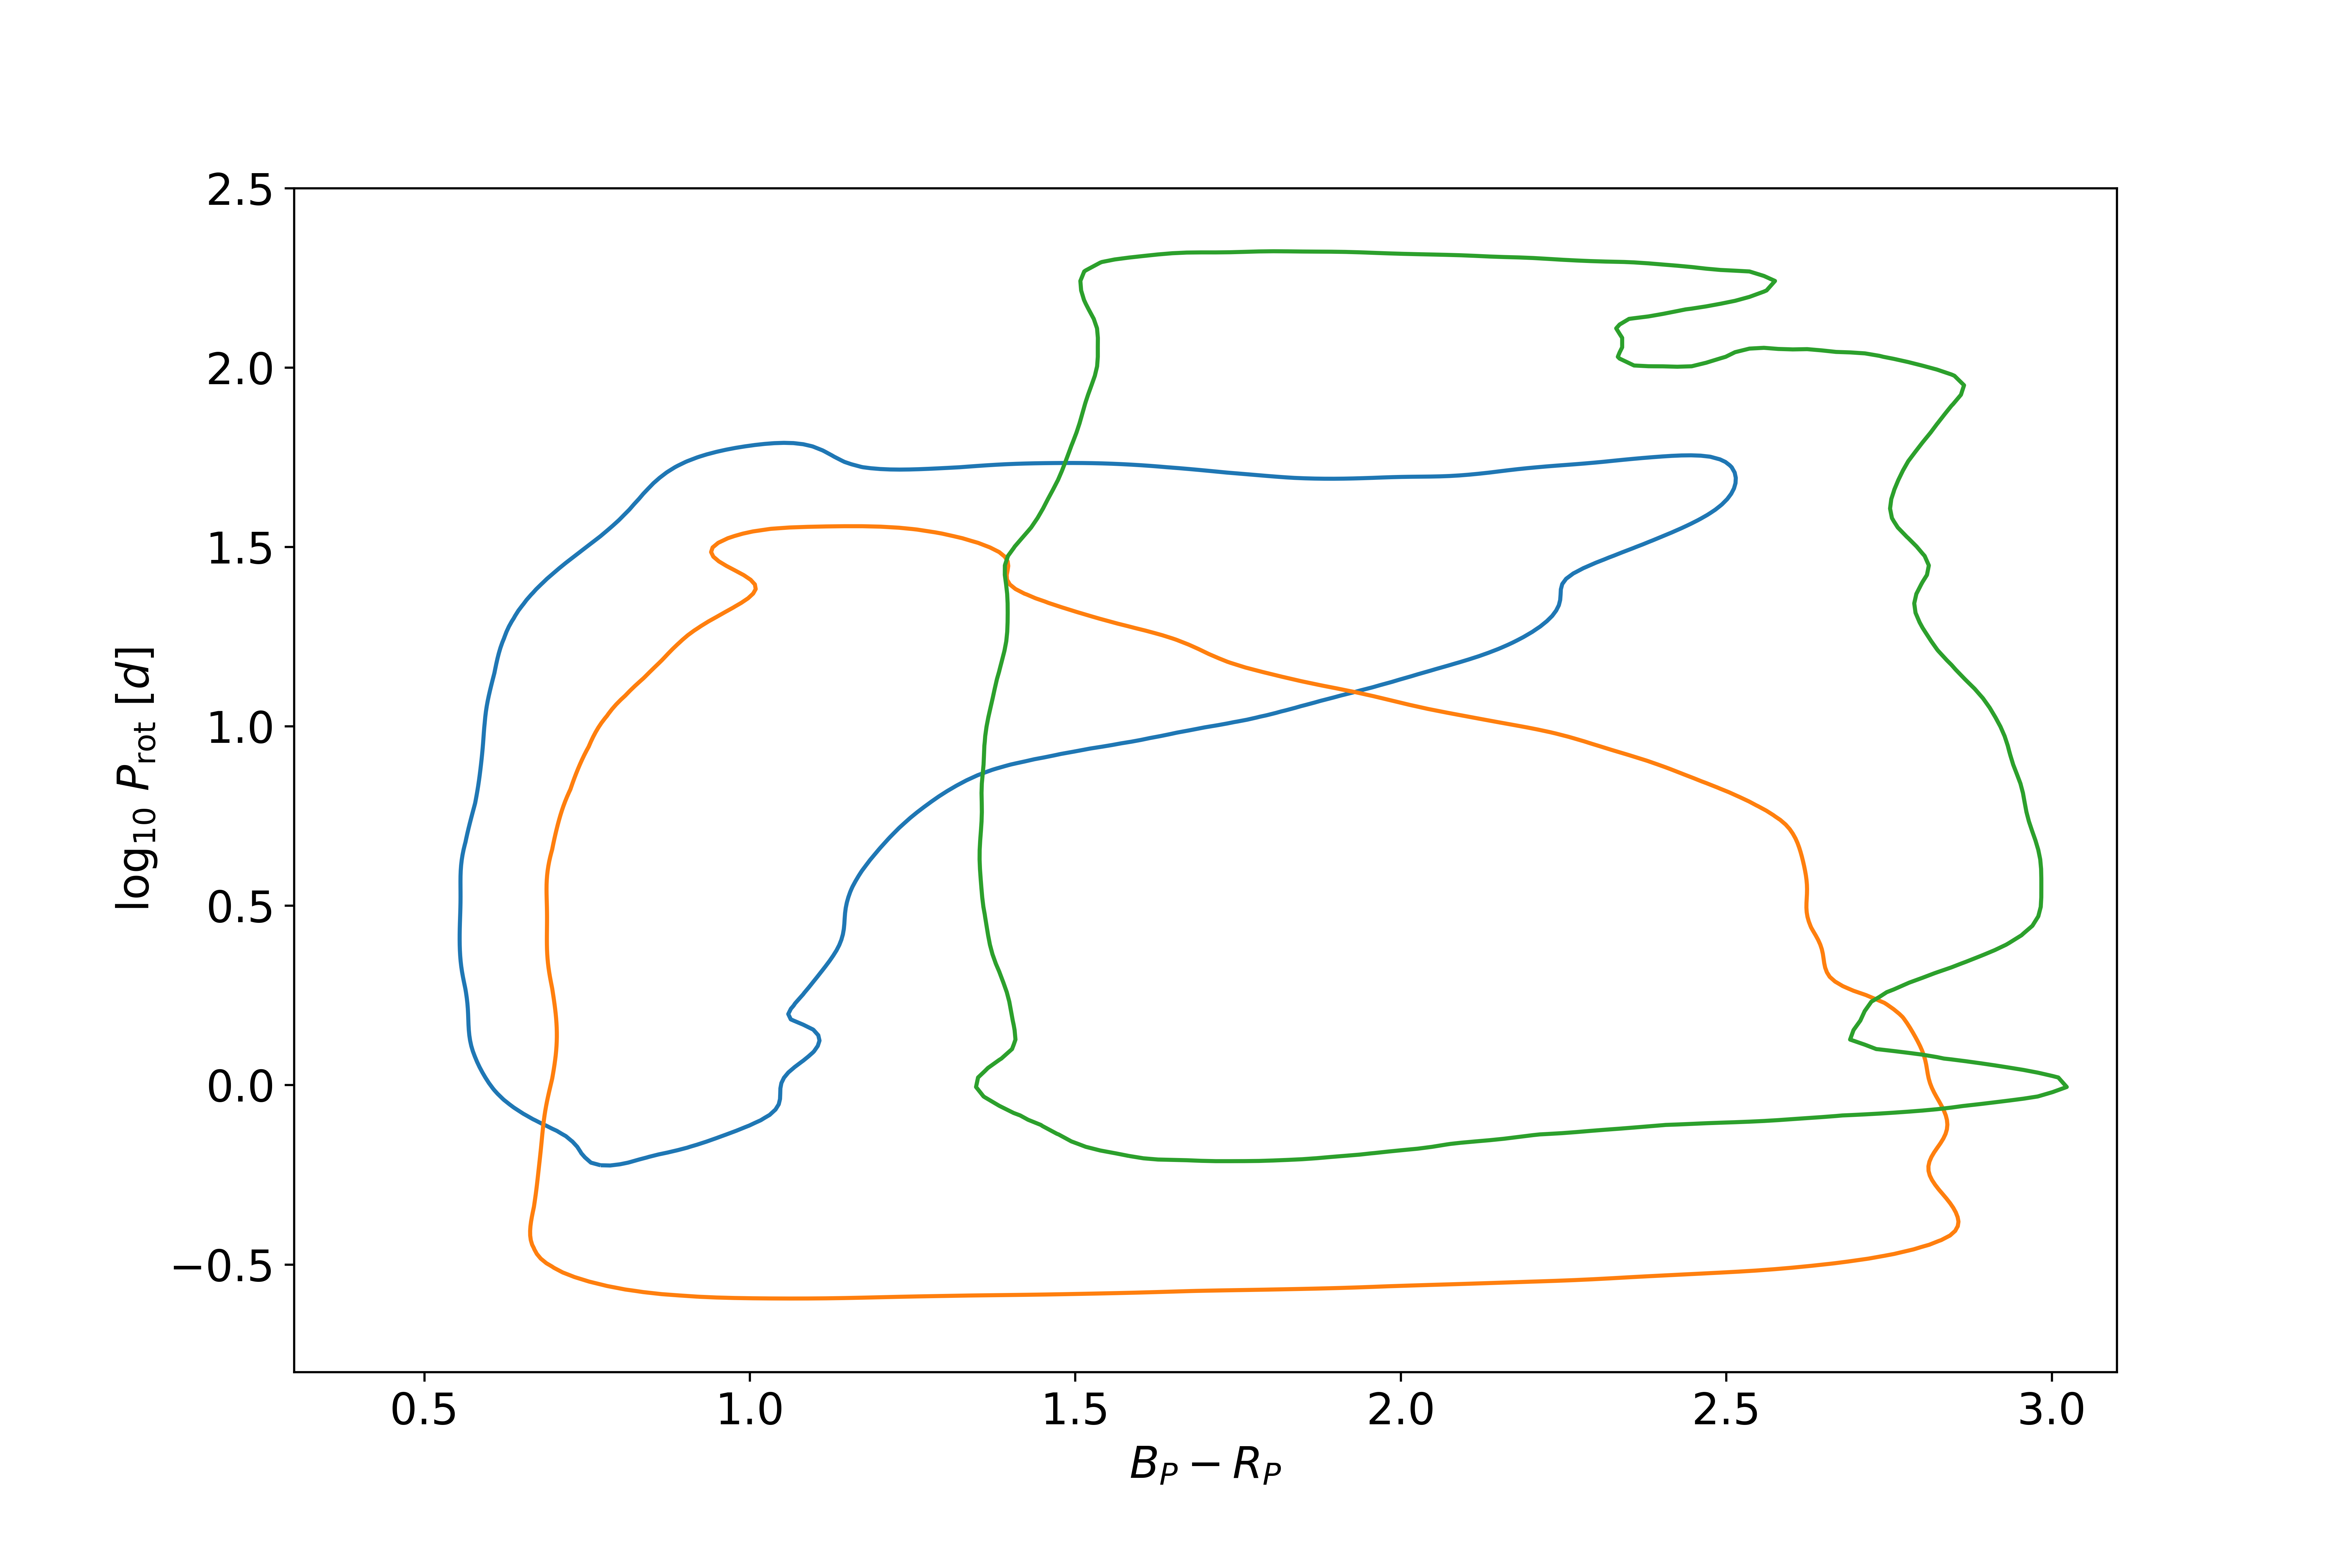
\includegraphics[width=\textwidth]{Figures/intro_figures/rot_comp.png}
    \caption{Normalised 2D histograms of the \kepler{} \citep{mcquillan_rotation_2014} (Top), \gaia{} DR3 \citep{distefano_gaia_2022} (Middle), and Zwicky Transient Facility (\ZTF) \citep{lu_bridging_2022} (Bottom) samples. Each sample probes a different area of the rotational period against colour space with some overlap. This expands our knowledge of the evolution of rotation to different types of stars while the agreement between these samples confirms their independent accuracy.}
    \label{fig:rot_comp}
\end{figure}

The stellar spot rotation periods that are obtained from each of these missions are suited to observe particular masses and rotation period regimes along the main sequence.
This results from the underlying telescope parameters, the scanning technique employed, and each mission's observation cadences \citep{distefano_determination_2012}.
Comparing the rotational period distributions in Figure \ref{fig:rot_comp} we observe a few notable features and limitations from each mission.
The Gaia DR3 rotation period sample exhibits spurious periods centred around 0.5, 18, 25, 32 and 49d.
\citet{distefano_gaia_2022} suggest that the non-uniformity of the Gaia sampling could be the cause of these peaks.
\kepler{} mainly targeted solar-like stars.
As a result, in the \kepler{} sample, there is a lack of measured periods for M dwarfs and fast-rotating young stars.
On the other hand, the \ZTF{} and \gaia{} samples did not have this targeting bias.
As a result, the \ZTF{} and \gaia{} samples probe the rotation periods of the comparatively lower-mass (redder) stars.
The Gaia DR3 rotation sample is, as a result of the Gaia scanning law, mostly suited to detect periods of rapidly rotating stars (P $<$ 5 d).
Due to the long observation baseline, the \ZTF{} mission was more suited to observe longer rotation periods.
Combining the results of these missions, we can accurately probe the evolution of rotation along the main sequence for a wider range of stellar parameters than the individual missions permit.
Further, the cross-match of stars between these missions confirm whether the individual missions themself provide accurate measures of the stellar surface rotation period.

Most of what we know about main-sequence rotational evolution arises from measuring stellar spot rotation periods.
However, the technique is limited by the requirement for stars to express stellar spots to be effective - a limitation that is invoked several times to explain phenomena discussed later in this Section. 
\citet{mcquillan_rotation_2014} attempted to measure the stellar spot rotation periods of solar-like stars in the \kepler{} sample.
In this work, they recovered the rotation period of ~20\% of stars with long cadence observations -~34000 detected rotation periods out of ~133000 selected stars in the sample.
On the other hand, \citet{distefano_gaia_2022} places the efficiency of the Gaia DR3 period detection pipeline at ~0.4\%.
They argue that the detection efficiency is non-constant and, in fact, a function of stellar magnitude, the amplitude of the rotational modulation, the stellar rotation period and the ecliptic latitude.
There may be regions of evolution where the stellar spot rotation period does not effectively probe rotational evolution.

All matter in the universe has some angular momentum. 
Stars are born in the core of spinning molecular clouds from the infall of matter due to gravity. 
As a result, all stars are rotating.
The amount of angular momentum a star is born with may depend on the cloud from which it was formed.

At the beginning of the  pre-main-sequence (PMS) phase, a young star is typically surrounded by a disk of gas and dust from which it is accreting material.
The accretion process can lead to an increase in the rotation rate of the star, as the angular momentum of the infalling material is transferred to the star.
However, as the star grows in size and mass, its magnetic field becomes stronger, which can slow down its rotation through the process of magnetic braking.

One key feature of PMS rotational evolution is the "disk-locking" phenomenon, in which the star's rotation becomes locked to the rotation of the disk \citep{eggenberger_angular_2012}.
This occurs when the star's magnetic field is strong enough to interact with the disk, causing the star and disk to rotate together.
Disk-locking can help to explain why some PMS stars have relatively long rotation periods, even though they are young and should be rotating rapidly due to the effects of accretion.

The interplay between accretion and magnetic braking can result in a complex evolution of the rotation rate of a young star during the PMS phase \citep{gallet_improved_2013}.
Observations of young stars in star-forming regions have revealed that the rotation rates of PMS stars span a wide range, with some stars spinning rapidly and others rotating slowly.
We show this complex relationship in Figure \ref{fig:pms_ms_evo}.
Comparative to the main-sequence where stars generally spin-down due to surface winds, the median rotation rate of PMS cluster is relatively constant with age.

\begin{figure}
    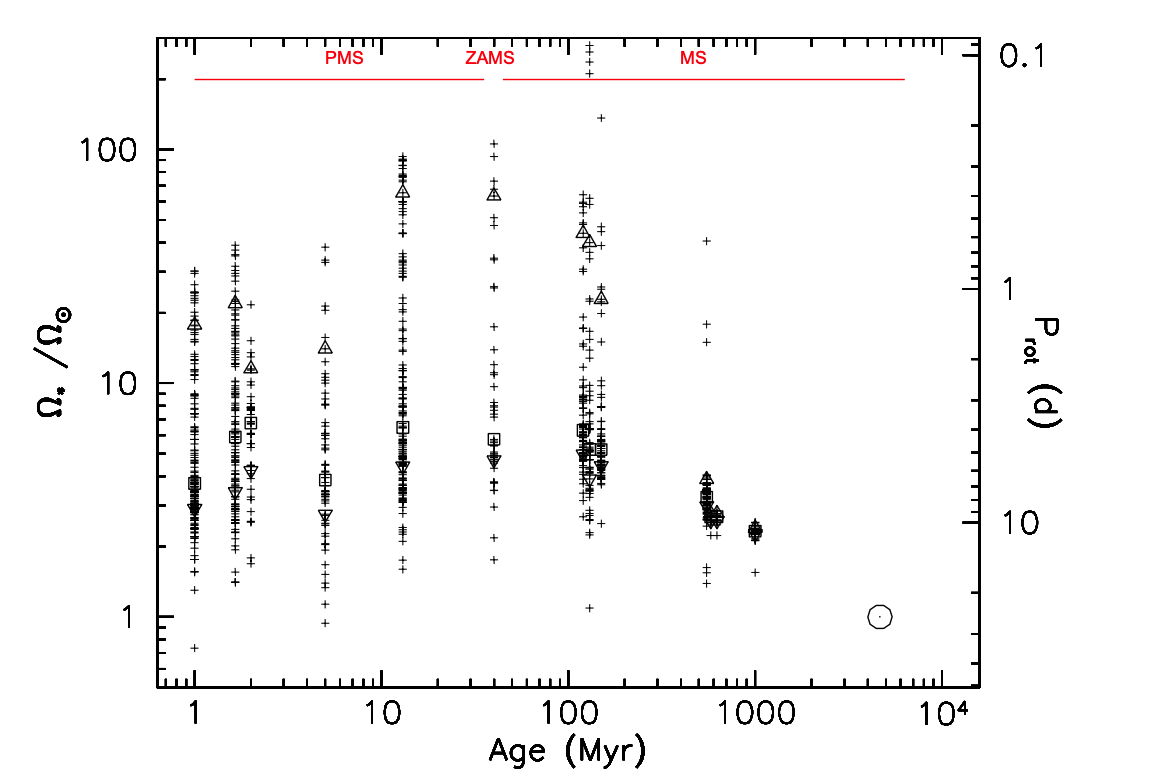
\includegraphics[width=\textwidth]{Figures/intro_figures/pms_evo.png}
    \caption{Angular rotation rate (relative to solar) distributions of low-mass young open clusters and the Sun. Triangles, inverted triangles, and squares represent the $90^{th}, 25^{th},$ and median rotation rates of the cluster. Open circle denotes the present value of the rotation rate of the Sun. Median values indicate that the rotation rate of cluster is approximately constant with age, despite the spin up by accretion. In order of increasing age (left to right) the clusters are ONC (1 Myr) \citep{herbst_stellar_2002}, NGC 6530 \citep{henderson_time-series_2012}, NGC 2264 (2 Myr) \citep{affer_rotation_2013}, NGC 2362 (5 Myr) \citep{irwin_monitor_2008}, h PER (13 Myr) \citep{moraux_monitor_2013}, NGC 2547 (40 Myr) \citep{irwin_monitor_2008}, Pleiades (120 Myr) \citep{hartman_large_2010}, M50 (130 Myr) \citep{irwin_monitor_2009}, M35 (150 Myr) \citep{meibom_slar_2009}, M37 (550 Myr) \citep{hartman_deep_2009}, Praesepe (578 Myr) \citep{delorme_stellar_2011}, Hyades (625 Myr) \citep{delorme_stellar_2011}, and NGC 6811 (1 Gyr) \citep{meibom_kepler_2011}.  Sourced from \citet{gallet_improved_2013},  Figure 1.}
    \label{fig:pms_ms_evo}
\end{figure}

While the many main-sequence stars have had their rotation rates measured, their ages are not well-constrained.
Resultingly the evolution of rotation with age is also not well-constrained.
Observations of young open clusters' main-sequence surface rotation from the \kepler{} mission suggest that angular momentum transport over a star's lifetime is consistent between clusters - the distribution of rotational periods of stars has considerable overlap between clusters \citep{spina_how_2020, curtis_when_2020}. 
Figure \ref{fig:cluster_rotational_periods} shows the distribution of rotation rates of some open clusters.
In this Figure, we can observe some significant aspects of the evolution of angular momentum in stars.

\begin{figure}[h]
    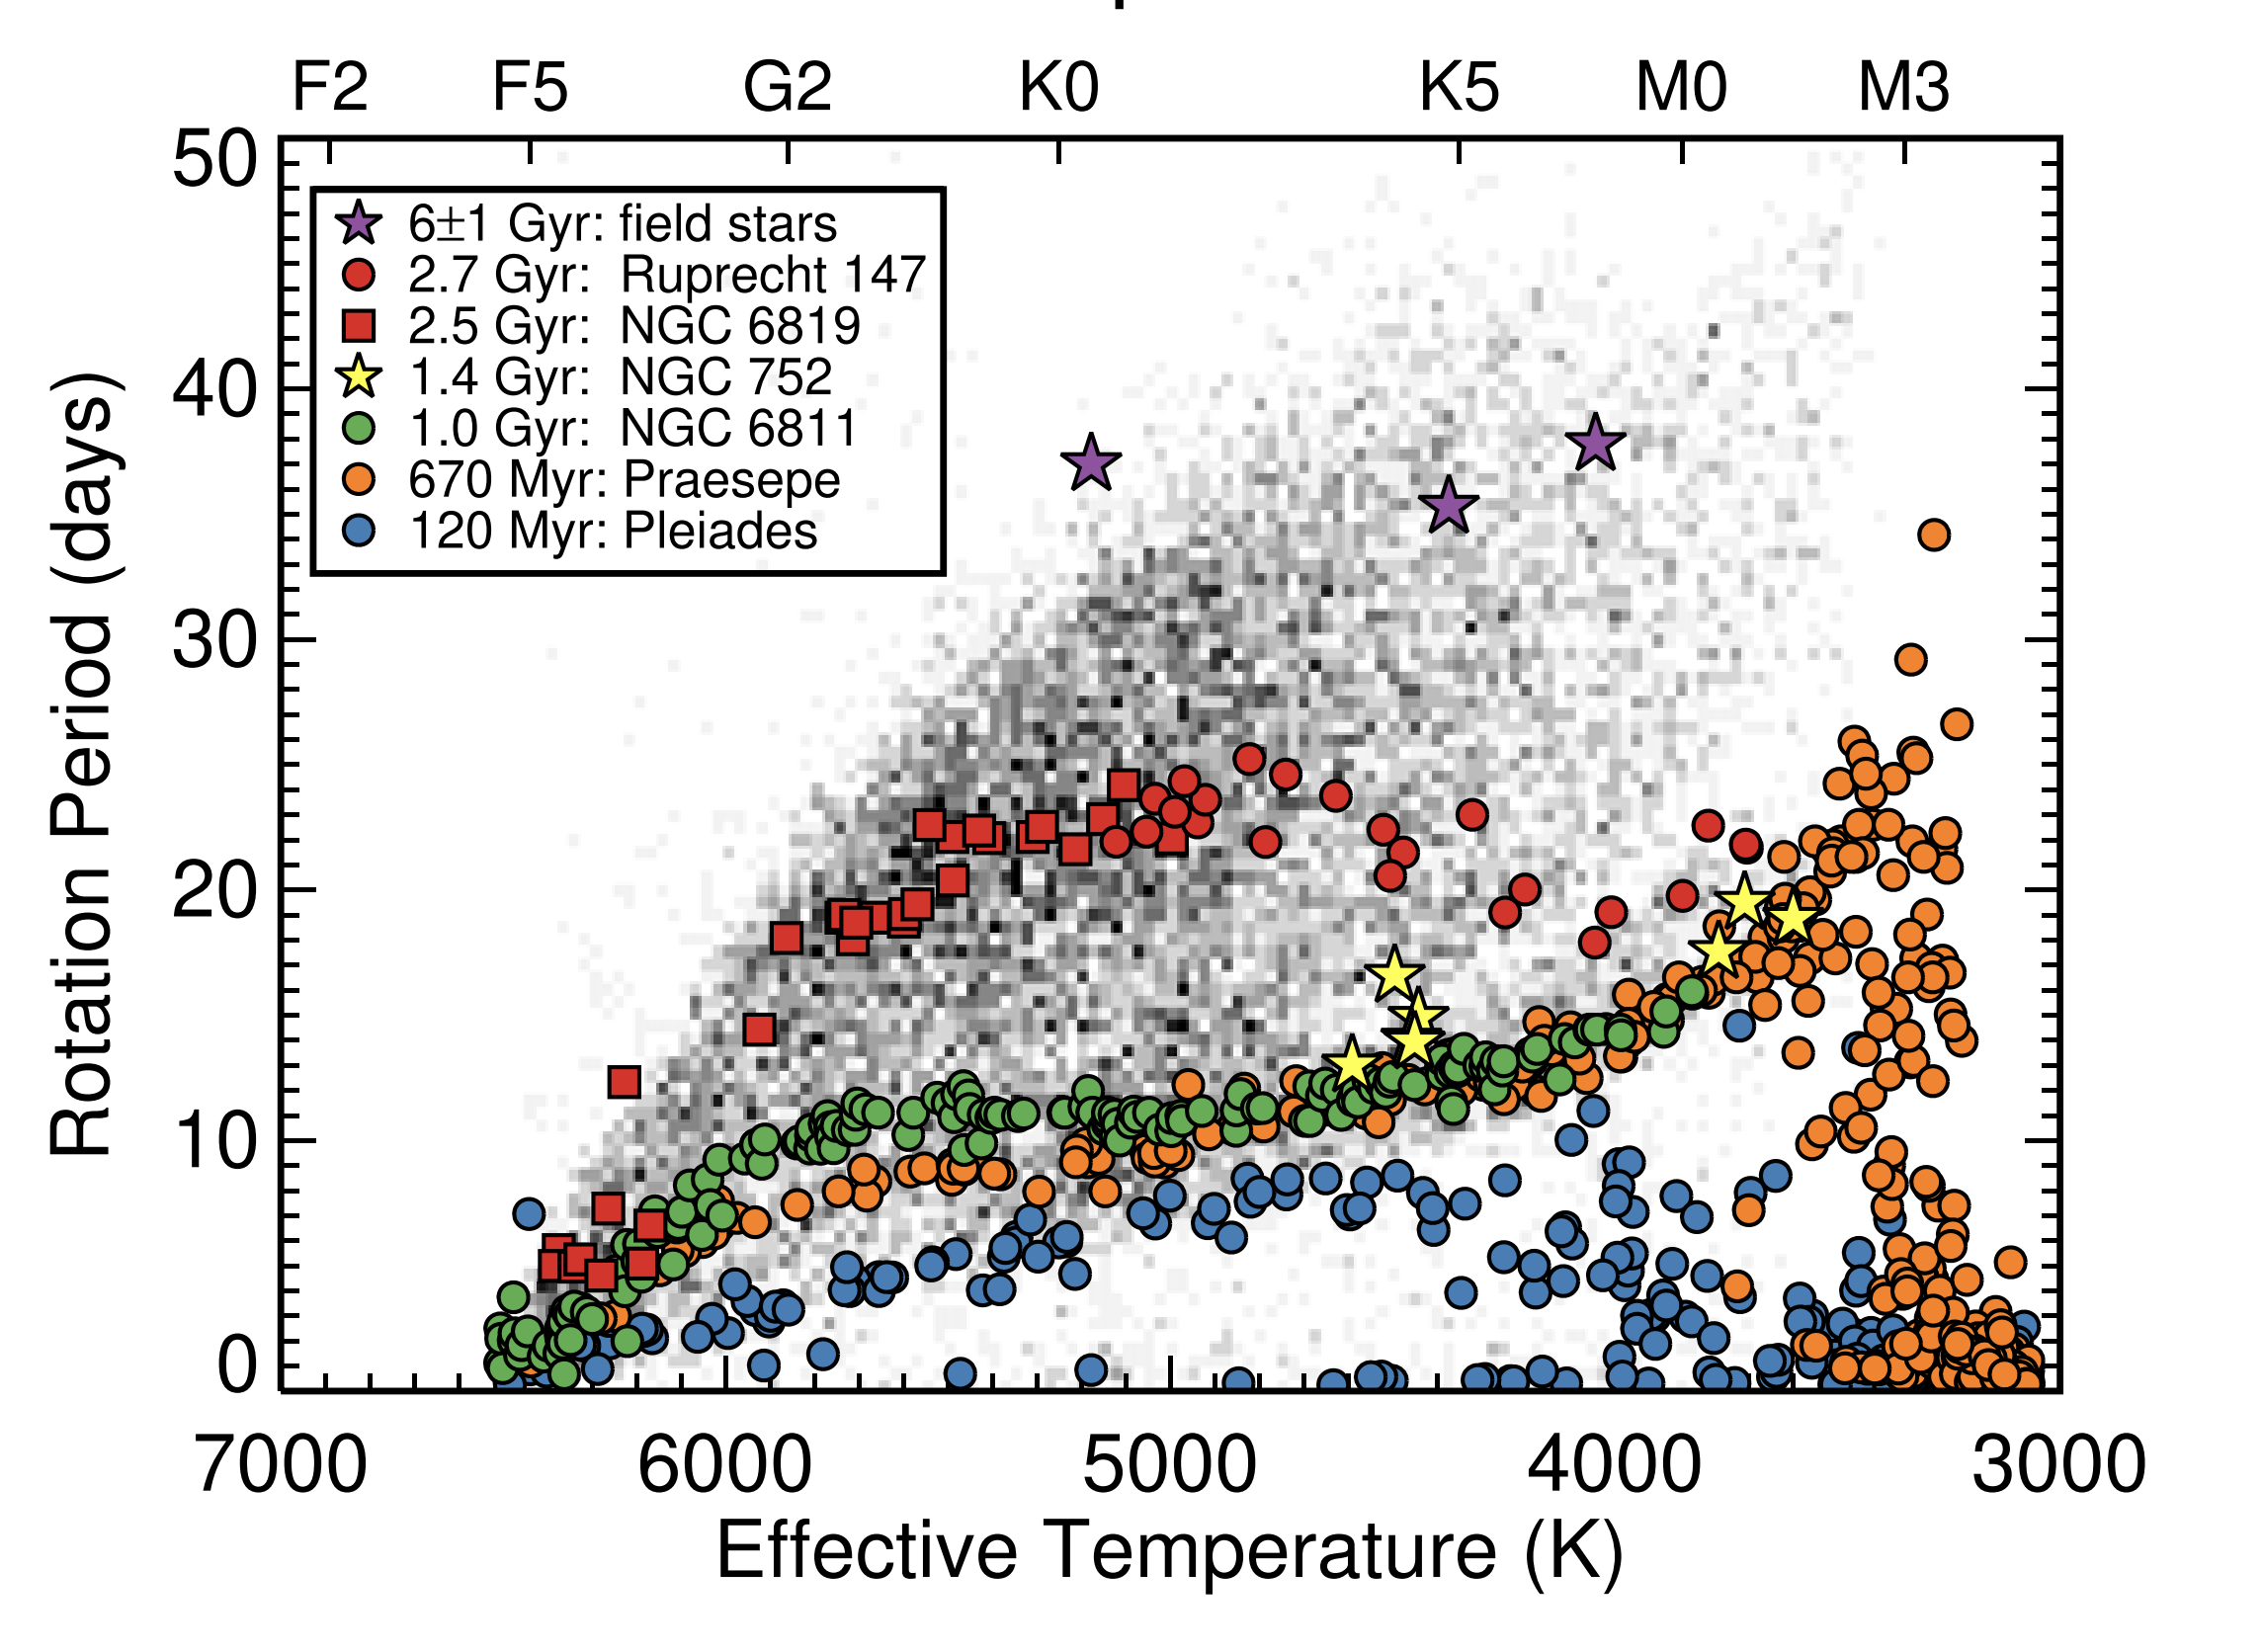
\includegraphics[width=\textwidth]{Figures/intro_figures/cluster_kepler.png}
    \caption{Scatter plot of various cluster rotational periods against effective temperature overlayed on the \kepler{} \citet{mcquillan_rotation_2014} rotational period sample.
    The agreement between low mass Praesepe and NGC6811 periods implies mass dependent core-envelope coupling for young ($<$1 Gyr) stars.
    Sourced from Top left panel of Figure 7 in \citet{curtis_when_2020}}
    \label{fig:cluster_rotational_periods}
\end{figure}

The surface rotational period increases over time for stars between $<$1.1 $M_{\odot}$.
Within this range of masses, angular momentum is lost from the convective surface through mass loss and interactions of the star's magnetic field and the lost ionised material through stellar winds - magnetic braking.
Through observations of the Pleiades, Ursa Major, and Hyades stars and the Sun, \citet{skumanich_time_1972} derived the proportional relation between the rotational rate of stars and the inverse square of their age - $\omega(t) \propto t^{-1/2}$.
This proportionality forms the standard for expected rotational evolution and for what is known as gyrochronology - measuring the ages of stars from their rotational rate.

Outside the $\sim$0.4 and 1.1 M$_{\odot}$ range, the rotation period also decreases, albeit slower, with much more complex relationships with time.
Above $sim$ 1.1 M$_{\odot}$, known as the Kraft break, stars have shallower convective envelopes and are believed to have less efficient magnetic dynamos - which induce strong magnetic fields.  
Resultingly, the magnetic braking in these stars is less efficient, and these stars continue to rotate rapidly throughout most of their main-sequence lifetimes. 
Below 0.4 M$_{\odot}$ stars are fully convective.
Angular momentum is efficiently transported throughout the star.
A greater amount of angular momentum needs to be removed to slow the star's rotational rate, compared to stars that are not fully convective.
The main-sequence rotational evolution of stars with mass $>$1.3 M$_{\odot}$ is unprobed.
Above this mass, stars have no convective envelope, and thus, they do not express stellar spots nor solar-like oscillations that can be used to probe the surface rotation rate.
Theoretical modelling of the rotational evolution of high-mass stars is a substantial area of research in which observations of stellar parameters such as chemical abundances must independently constrain angular momentum transport rather than observations of stellar rotation.
As this work has a stronger focus on observing the rotation of stars, these results will not be discussed here.
For more information, we suggest reviews of astrophysical models of high-mass stellar rotational evolution, e.g. \citet{heger_presupernova_1998,maeder_evolution_2000,maeder_physics_2009}.

Until recently, it was assumed that there was little to no angular momentum transport between the radiative core and convective surface of main-sequence stars in the 0.4 - 1.1 M$_{\odot}$ range. 
Helioseismic observations of the Sun suggest that only the stellar surface undergoes rotational braking, and the core remains rotating rapidly - suggesting minimal angular momentum transport between the core and the surface on the main sequence. 
However, open cluster rotation period observations suggest that Skaumanich-like rotational evolution alone does not explain the observed distributions of rotation periods with mass.


\citet{spada_competing_2020} proposed that mass-dependent angular momentum transport between the core and the surface was required to explain observations of young ($<$ 1 Gyr) open cluster rotation period distributions.
In their work, they argue that clusters contain two sequences of stars: a sequence of relatively slower rotators, following the expected coherent slowing of rotation rate following the Skaumanich relation, and a sequence of lower mass stars that appear to have a constant rotation rate between clusters of different ages.
They compared the observations of the $\sim$700-Myr old Praesepe and the 1-Gyr old NGC 6811 clusters.
Figure 1 in \citet{spada_competing_2020} compares the rotation period distribution of the Pleiades (120 Myr), Praesepe (670 Myr), and NGC 6811 (1 Gyr).
Comparing observed rotation periods, they find that higher mass stars ($>$ 1 $M_{\odot}$) that are on the slow rotator sequence of the older NGC 6811 have longer periods than their counterparts in the younger Praesepe, as Skaumanich rotational evolution suggests.
On the other hand, the two clusters' rotational periods are indistinguishable at lower masses ($<$ 0.8 $M_{\odot}$)
In other words, low-mass stars have not been spinning down at all in the intervening 300 Myr. 
They argue that behaviour manifests mass-dependent core-envelope coupling - angular momentum transport between the core and the surface - briefly compensating for the loss of angular momentum due to wind braking at the surface.
They develop a semi-analytical model of the rotational period's evolution with a star's age and mass tuned with the observations of stellar cluster rotational period distributions.
This notably improves the accuracy of gyrochronology compared to the Skaumanich relation, especially for younger low-mass stars.

On the other hand the slow spin down rates of fast rotating stars could be related to saturation of the angular momentum loss due to stellar winds for fast rotating stars \citep{johnstone_stellar_2015, johnstone_stellar_2015-1,gallet_improved_2013}.
This is motivated by the saturation of magnetic field indicators for fast rotation rates - or rather low Rossby numbers \citep{wright_stellar-activity-rotation_2011}.
This could explain the slower observed spin-down of young rapidly rotating stars.
Both of these prescription neglect the each other: \citep{spada_competing_2020} includes a simple stellar wind prescription that does not consider the saturated regime, while \citep{gallet_improved_2013} does not consider mass dependent angular momentum transport within the star.

Another phenomenon not well explained by Skaumanich-like rotational evolution is the observed intermediate period gap.
\citet{mcquillan_rotation_2014} calculated the rotation periods of ~30000 stars in the \kepler{} sample from photometric oscillations of surface brightness from stellar spots.
The distribution of the log of the rotational periods from this sample against their colour is shown in Figure \ref{fig:kepler_rot_period}. 
Following increasing rotation period as a proxy for time, this Figure highlights the overabundance of observations followed, temporally, by a dearth of observations of particular rotational periods - the position of which varies with mass.

\begin{figure}[h]
    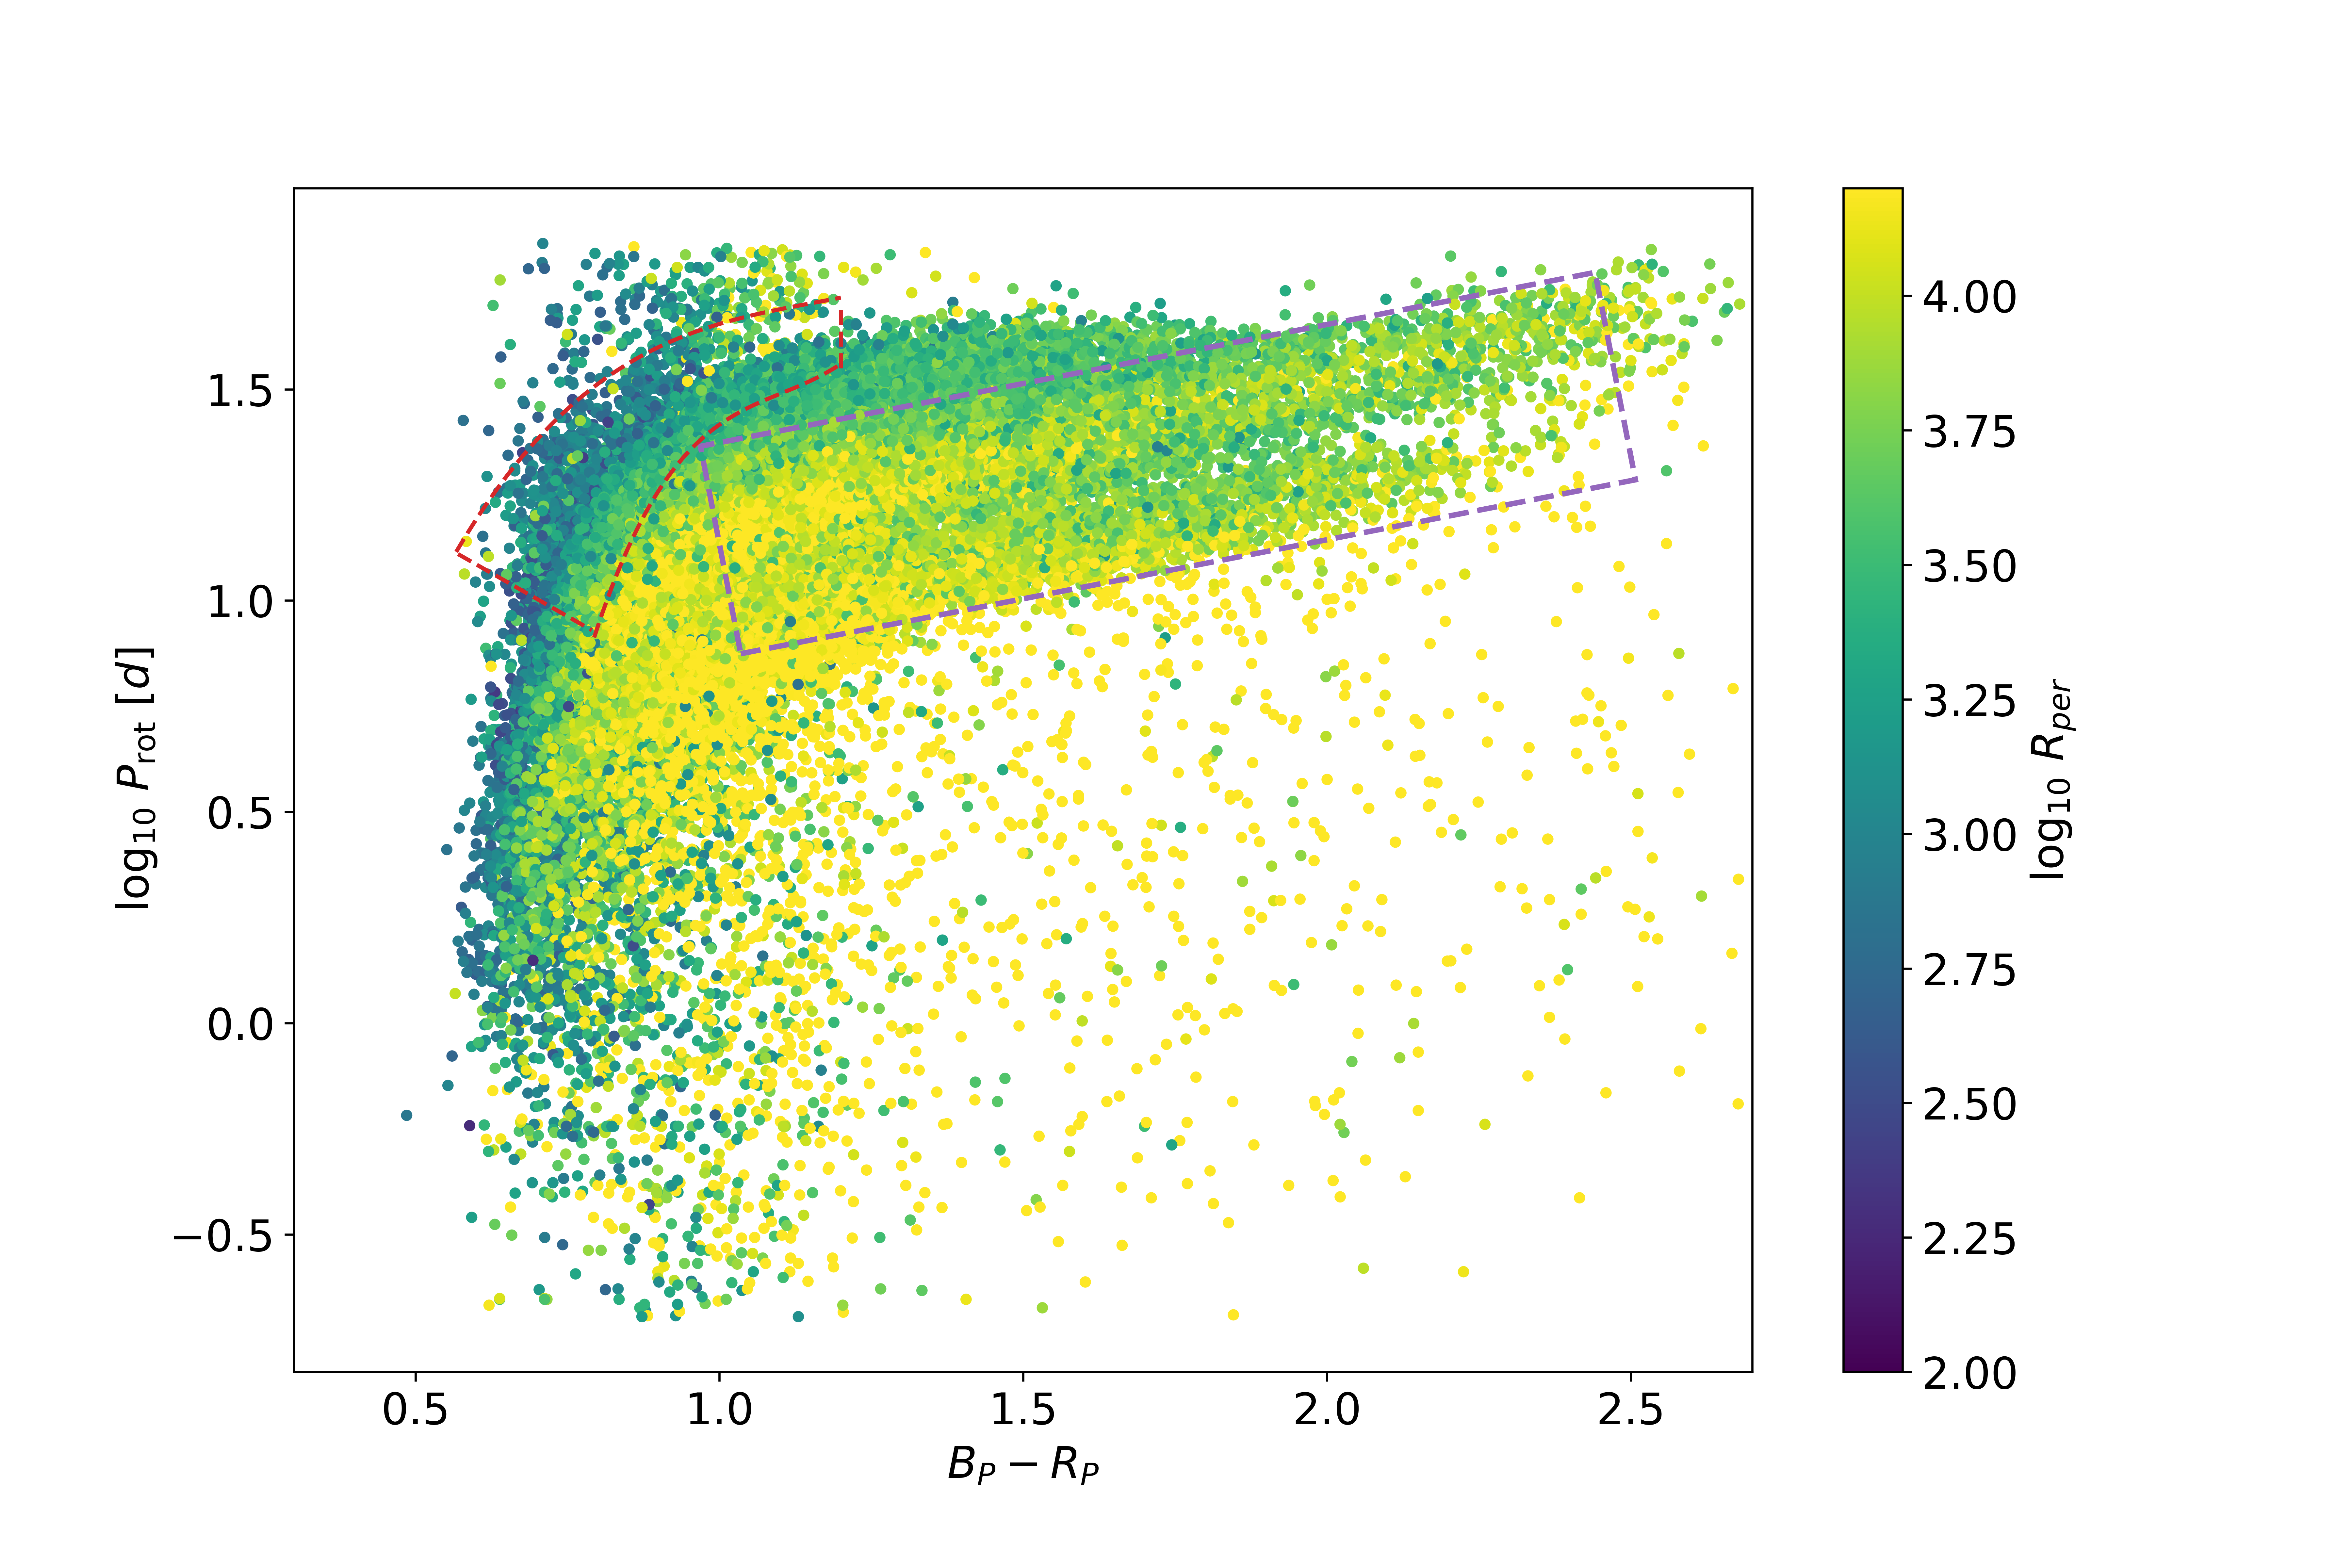
\includegraphics[width=\textwidth]{Figures/intro_figures/kepler_rot_dist.png}
    \caption{Scatter plot \gaia{} $B_P-R_P$ colour against log of the rotational period of the \kepler{} \citet{mcquillan_rotation_2014} rotational period sample coloured by the log of the photometric variation ($R_{var}$).
    $R_{var}$ decreased towards the gap from above and below, suggesting the intermediate period gap is representative of a minimum of observability of rotation period. Highlighted by arrows in this Figure are two features that we discuss in more detail in this Section: the intermediate period gap and the long-period pile-up.}
    \label{fig:kepler_rot_period}
\end{figure}

Since identifying the gap, several explanations have been presented for this phenomenon.
\citet{mcquillan_rotation_2014, davenport_rotating_2017} first proposed that rather than the gap being the result of modified angular momentum transport, the gap is the artifact of a recent period of bursty star formation in the \kepler{} field - resulting in a young ($<$ 50 Myr), fast rotating, population and older, background slowly rotating, population.
\citet{davenport_rotating_2017} further find that the fast and slow rotators in his sample also exhibit a different distribution of the proper motion.
Two kinematically separate groups favour the explanation of two epochs of star formation in the \kepler{} field. 
This explanation is further supported by the work of \citet{davenport_rotating_2018}, who showed that the gap appears to correlate with Galactic height, which is assumed to be related to stellar age.

The recent bursty star formation hypothesis accounts for the overpopulation of observations below the gap. 
In contrast, the dearth of observations represents the background observation rate of rotational periods within this period range.
\citet{gordon_stellar_2021} provided evidence against this hypothesis through analysis of \ktoo{} data.
They found that the intermediate period gap is present in the multiple pointings of the \ktoo{} mission - suggesting that recent bursty star formation is isotropic -  and that clusters with different ages contain stars that have crossed the gap.

The former suggests that all clusters universally went through a period of bursty star formation $\sim$50 Myr ago. 
\citet{angus_exploring_2020} observed that the velocity dispersions of stars increase smoothly across the gap.
Given that the two populations - above and below the gap - do not substantially differ in other spectroscopic and photometric observations, this scenario remains theoretically possible but unlikely.
The latter requires slightly more thought. Comparing Figures \ref{fig:cluster_rotational_periods} and of \ref{fig:kepler_rot_period}, the gap has a sharper slope than the sequences associated with constant age populations from Praesepe \citep{douglas_poking_2017,douglas_k2_2019}, NGC 6811 \citep{curtis_temporary_2019} and Ruprecht 147 \citep{curtis_when_2020}. 
If the bimodal star formation scenario explained the gap, the gap should have the same shape and position for each cluster and the entire \ktoo/\kepler{} sample.

Before exploring possible explanations for the intermediate period gap, it is worth identifying where the rotational period gap occurs in the stars' evolution.
\citet{reinhold_transition_2019} first suggested that the gap aligns with a rotational isochrone at $\sim$ 800Myr.
With \citet{spada_angular_2016} modifications to Skaumanich spin down for low-mass star to reflect the rotational distribution of clusters of known age, updated the proposed age to ~750 Myr \citep{reinhold_transition_2019}.
Contrary to the hypothesis that the gap aligns itself with a certain isochrone, \citet{curtis_when_2020} identified that the open cluster Ruprecht 147 contains stars above and below the gap - as well as one star that appeared to be within the gap.
This suggests that the gap does not align itself with a particular age.
Instead, they argued that the gap aligns itself with a line of constant Rossby number\footnote{Defined as the ratio of the rotational period to the convective turnover timescale ($Ro = P_{rot}/\tau_{conv}$) - which itself is dependent on mass and is approximately constant for a star's main-sequence lifetime} = 0.5.
The Rossby number is associated with the magnetic dynamo, e.g. \citet{noyes_rotation_1984, montesinos_new_2001, augustson_rossby_2019}
To simplify, a star can be thought of as a volume of charged particles.
As a star rotates, so do the charged particles within it.
Moving charged particles induce a magnetic field - creating a magnetic dynamo.
As the star rotationally evolves, so does the magnetic dynamo.

Given that the gap appears to line up with a line of constant Rossby number, this may suggest that the gap is instead caused by an event in the evolution of the magnetic dynamo rather than an event in time.
This is a notable result because the magnetic dynamo is associated with a number of stellar phenomena - such as magnetorotational instabilities (angular momentum transport processes associated with the magnetic field) or stellar spots.

Other prospective hypotheses for the intermediate period gap can be broken down into two categories: (1) modified angular momentum transport and (2) decreased observability of rotation periods.

Let us consider the first hypothesis: the gap results from modifications to angular momentum transport.
\citet{lu_bridging_2022} have shown that the gap is most apparent for stars less massive than 1.3 M$_{\odot}$ and more massive than 0.4 M$_{\odot}$.
If we look closely at Figure \ref{fig:ztf_comp} we can see that for the \ZTF{} sample (black dots) the intermediate period gap is most apparent for stars 1.5$<B_P-R_P <$2.5 and closes for low mass ($B_P-R_P >$2.5) stars.
Stars redder than $B_P-R_P >$2.5 are fully convective \citep{amard_first_2019}, suggesting that the gap may be another phenomenon related to the interplay between angular momentum transport between the radiative core and convective surface and surface rotational braking along the main sequence.

\begin{figure}[h]
    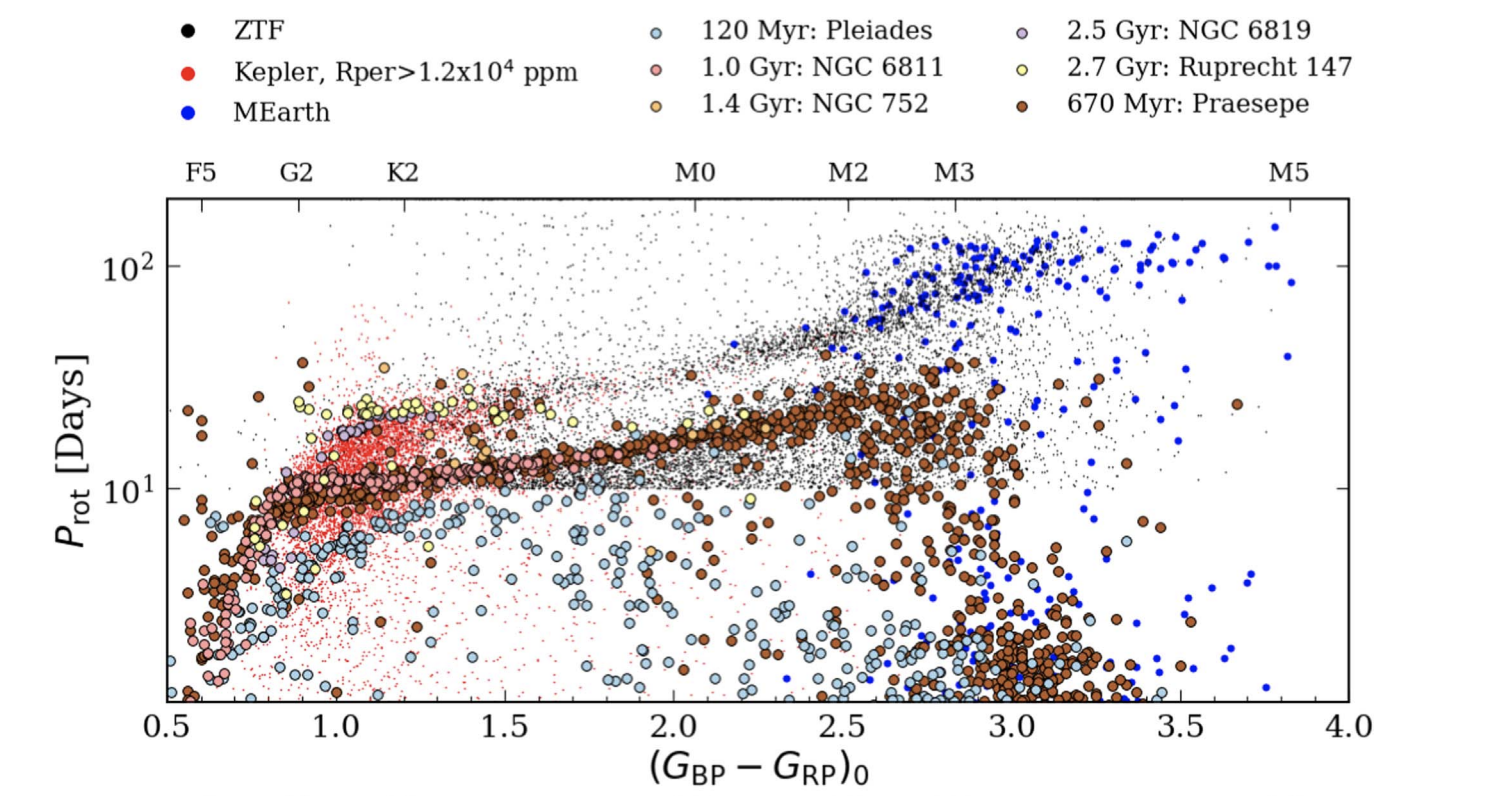
\includegraphics[width=\textwidth]{Figures/intro_figures/ztf_comp.png}
    \caption{Rotation period against \gaia{} $B_P - R_P$ from \kepler{}, \ZTF{} overlayed with various open cluster measurements. Highlighted by this Figure is the disappearance of the intermediate period gap above $B_P-R_P$ = 2.5 - the fully convective star boundary. This suggests that the rotational period gap is related to the coupling of the core and surface of low mass stars (0.4 $M_{\odot}<M<1.3M_{\odot}$). Sourced from the top panel of Figure 8 in \citep{lu_bridging_2022}.}
    \label{fig:ztf_comp}
\end{figure}

\citet{mcquillan_rotation_2014} first proposed that the gap is the result of two variations to Skaumanich rotational evolution.
First, stars below the gap undergo a period of stalled spindown, resulting in the observed overdensity of stars along the lower branch, followed by a period of accelerated spindown, resulting in the dearth of stars in the gap\footnote{The authors disfavoured the hypothesis favouring the bimodal star formation hypothesis discussed earlier in this work.}.

The proposed mechanism underlying this scenario is the mass-dependent decoupling and recoupling of the core and the envelope proposed in 
\citet{lanzafame_rotational_2015} and \citet{spada_competing_2020}, discussed earlier in this work.
\citet{angus_exploring_2020} suggest that the core envelope decoupling and recoupling may explain the period gap as a break between a "younger" pile-up regime (Ro$<$0.6) in which surface rotation periods are relatively constant with time from core-surface angular momentum transport and increase with decreasing mass from an "older" (Ro$>$0.6) regime with the gap representing a period of relatively fast spin evolution during the transition between the two.
Proponents of this hypothesis suggest that the gap results from a period of enhanced spindown following core and surface recoupling where stars "jump" the gap before resuming Skumanich spindown, as is observed for older clusters.
Models of - and physical mechanisms underlying - rotational evolution that reflect the proposed rapid spindown are yet to be identified.
Under this model, the gap reflects an under the density of stars but would not be empty.
There should be a small number of stars with Ro $\approx$ 0.6, irrespective of our ability to measure their rotational periods.
\citet{curtis_when_2020} found five Ruprecht 147 stars in or just beneath the gap yet to be thoroughly investigated.

Now let us discuss the second hypothesis: the gap results from a lack of observations of rotational periods.
The rotational period of \kepler{} stars requires that stars express photometric oscillations from stellar spots.
Starspots are regions of intense magnetic activity on a star's surface from magnetic flux tubes in the convection zone. 
These flux tubes are thought to be stretched and curled by the differential rotation of the convective region. 
As a result, convection is inhibited, limiting plasma flow to the surface in these tubes.
This results in lower-temperature material within the tube, which looks like a darker spot on the star's surface.
Stellar spots have bright perimeters surrounding the cooler internal regions of spots, known as faculae.

Stellar spots can both increase or decrease stars' bolometric luminosity.
 \citet{reinhold_fast_2013} and \citet{reinhold_transition_2019} propose that the gap represents the transition in stellar spot structure from spot to faculae dominance in the photosphere.
Following their explanation, the gap corresponds to a transition where the increase in bolometric luminosity from the faculae negates the decrease from the internal, cooler region of the stellar spots. 
In the \citet{mcquillan_rotation_2014} sample, stellar rotational periods are measured from the period of brightness variability due to the brightness variability introduced by stellar spots\footnote{this technique is discussed in more detail in Section \ref{sec:stellar_spot_brightness_modulations}}.
Suppose the bolometric flux does not vary due to stellar spots in the gap region. 
In that case, the amplitude of periodic variability would decrease within this region.
\citet{reinhold_transition_2019} suggests that the gap is full of stars and represents a minimum in the detectability of rotation periods.

Supporting this hypothesis, in both the \kepler{} and \ktoo{} fields, the variability amplitude ($R_{var}$) decreases towards the gap from both lower and higher rotational periods.
This can be seen in Figure \ref{fig:kepler_rot_period}, which is coloured by the log of $R_{var}$.
On the other hand, while there is evidence that stars undergo spot-to-faculae dominance, e.g. the Vaughan-Preston gap \citep{vaughan_survey_1980}, this occurs much later in a star's lifetime at Ro $\sim$ 1.
Further, there is evidence that stars above and below the gap are both spot-dominated  \citep{lockwood_patterns_2007, reinhold_transition_2019}.
\citet{reinhold_transition_2019} speculate that activity cycles that vary the spot-to-faculae brightness contributions on rotational timescales could be the process underlying the rotational period gap.
As of writing, there is no evidence to support this hypothesis.

Recent works have attempted to identify the fractional spot coverage of cluster members from their spectra \citep{cao_starspots_2022}.
They do this by assuming the spectra of stars can be broken down into spot and ambient components that vary in temperature but are consistent in other stellar parameters.
They find that the fractional spot coverage of stars is related to the Rossby number.
Within this work, they observe a population of spot-coverage-enhanced stars that deviate from the relations they present.

In a follow-up work \citep{cao_core-envelope_2023} they combine the angular momentum transport and decreased observation hypothesis by proposing
that star spot measurements in the Praesepe open cluster are strongly enhanced only for stars that depart Skumanich rotational evolution.
They suggest that a decoupling of the core and the surface explain both observations.
In their model, angular momentum transport between the core and the surface slows the increase of the rotational period. 
The resultant shears enhance the magnetic dynamo and, thus, stellar spot activity.
Stars enhanced in stellar spot coverage are expected to have decreased observed effective temperatures.
Spot-dominated, as opposed to faculae-dominated, stellar spots are cooler than the ambient temperature of the star.
As a result, stars with enhanced stellar spot coverage have a decreased observed effective temperature.
They then speculate that the rotational period gap is thus the result of a bias in observed effective temperature rather than a lack of observations of the rotational periods of stars in the gap.

Observations of open cluster rotational distributions beyond the gap suggest that stars $<1M_{\odot}$ that have crossed the gap (Ro$>$0.6) continue to spin down and follow the Skumanich-like rotational evolution until they leave the main sequence.
On the other hand, there is an apparent overabundance of stars at critical rotation periods (dependent on their mass). 
Above this is a lack of observations of rotation periods for stars $>$5500K.
Stars with higher masses also appear to have lower rotation periods on the pile-up than their less massive counterparts.
This results in what is known as the long-period pile-up, as noted in Figure \ref{fig:kepler_rot_period}.
The long-period pile-up aligns itself in the \citet{mcquillan_rotation_2014} period distribution with Rossby number  (Ro = 2.08) \citep{van_saders_forward_2019}.
 
\citet{van_saders_forward_2019} suggest that the long-period pile-up could result from decreased magnetic braking or a lack of observations of stars beyond this Rossby number.
Under the former scenario, stars stop spinning down when they reach this Rossby number as a result of weakened magnetic braking.
This results in the overdensity of stars and a lack of observations of larger rotational periods.
In the latter, they propose that the error in observed periods can smooth out the overdensity of stars and, infact the lack of rotational periods is because of variations to the stellar spot activity (See above discussion of speculative explanations for decreased observation of rotational periods within the rotational period gap).
Further supporting this explanation \citet{david_further_2022} found that photometric variability decreases above the gap.
Suggesting an unobserved population of stars with longer rotation periods.

Under the weakened magnetic braking model \citet{david_further_2022} suggest that stars in this temperature regime $1M_{\odot} < M < 1.3M_{\odot}$ may spend half of their main-sequence lifetimes at the long period pile-up with only modest variances to their rotational period.
Below this mass regime, stars appear to continue to lose angular momentum through wind braking following the Skumanich relation.
This results in stars with large rotational periods when they enter the post-main-sequence.

%\todo write me
%\subsubsection{Latitudinal differential rotation}
%
%Another facet of differential rotation is latitudinal rotation.
%This is the observation that the rotation profiles of stars differentially rotate dependent on latitude.
%As we touched on earlier this was first discovered in the Sun, where the equator was found to be rotating with a period of 25 days at the equator and 38 days at its poles.
%The Sun is rotating equator-fast and therefore has a solar-like rotation profile.
%The inverse of this is stars that are rotating with equator-slow latitudinal differential rotation profiles, known as anti-solar-like rotation profiles.
%
%The latitudinal differential rotation of stars is difficult to measure and we will discuss the techniques adopted to measure differential rotation in more detail later in this 



\subsection{Post-main-sequence}

For low mass (1.1 - 1.5 M$_{\odot}$) stars during the post-main-sequence, the information provided to angular momentum transport by each star can be greater than during the main sequence.
While surface rotation rate can still be measured through stellar spot photometric oscillations, within this regime, the core and surface can also be simultaneously constrained through asteroseismology (at different points in evolution). 
This results from a combination of the expression of mixed modes, shorter mode lifetimes, and increased core rotation rates.
During the main sequence, g-modes are trapped within the radiative core and thus do not introduce brightness variations (oscillations) to the stellar surface.
Some g-modes can couple with p-modes in the surface convective cavity during the post-main-sequence and are known as "mixed modes".
The rotational splittings of the mixed modes allow us to infer the rotation rate in the radiative region and deep core. \citep{metcalfe_precise_2010,bedding_gravity_2011}
Where, precisely, the mixed modes probe is dependent on where in the post-main-sequence the star is observed.
For example, sub-giant stars express p-modes and mixed modes that can probe both the core and the surface, whereas red giant branch (RGB) stars mainly express mixed modes that can only probe the star's core.
While stellar spot surface rotation periods can be measured for post-main-sequence stars \citet{mcquillan_rotation_2014, ceillier_surface_2017}, asteroseimic inference of core and surface rates is the standard for probing rotation evolution in this evolutionary regime \citep{deheuvels_seismic_2014, gehan_core_2018, deheuvels_seismic_2020, fellay_asteroseismology_2021}.

Measuring the core and surface rotation rates simultaneously provides much more information to angular momentum transport than either of these quantities alone.
For example, during the main-sequence, the over-abundance of stars along the lower branch of the Kepler rotation period gap could simultaneously be explained by diminished wind braking for the surface or by core-envelope recoupling.
Measuring the core rotation rates would break this degeneracy.
This asteroseismic quirk is useful as it allows us to directly investigate angular momentum transport more efficiently.

However, the constraints to the rotation profile of stars by asteroseismology, even in the post-main sequence, are limited.
Indeed the core and surface rotation rates of subgiants can simultaneously be probed.
However, where in a star the rotation can be probed depends on the observed oscillation modes, which depend on the stellar structure.
The rotation rates obtained by asteroseismology are kernel-based averages of the rotation profile in regions that the observed oscillation modes probe.
For example, subgiants' core and surface rotation rates are the kernel-based average rotation rates of the innermost $r/R$<0.05 and outermost $r/R>0.9$ regions (on average).
Between these regions, the rotation profile is not constrained.
As a result, the shape of the rotation profile, which can be fingerprints of specific angular momentum transport mechanisms at play, is also not constrained.

Asteroseismic inference of rotation rates can also be imprecise.
This can be seen when comparing the surface rotation periods from asteroseismology and stellar spot photometric oscillations in \citet{hall_weakened_2021}.
This is because: a) state-of-the-art measurements of rotational splittings - the quantity that constrains the rotation profile - are low SNR and are often also imprecise, and b) the observed rotational splittings are a finite subset of the infinite number of rotational splittings that would be required to accurately and precisely constrain the entire rotation profile.
With these limitations in mind, we now discuss the observed evolution of rotation of post-main-sequence stars.

Following the main-sequence, low-mass stellar rotation varies with the evolutionary phase.
Models of rotating stellar evolution (e.g. )\citep{maeder_evolution_2000,heger_presupernova_2000} predict the following qualitative evolutionary pathway.
Towards the end of the main sequence the rotation profile is largely flat.
Assuming conservation of angular momentum as hydrogen core burning stops, pressure in the core drops, resulting in core contraction while the convective surface region expands.
Resultingly the core is spun-up while the surface is spun-down.
The core should continue to spin down as the core contracts along the RGB until entering the red clump (low-mass core He burning).
The core burning reintroduces core pressure, and the resulting expansion of the core decreases the core rotation rate.
When core He burning ceases, the core pressure drops again, resulting in a spun-up white dwarf (relative to the core rotation rate of red clump stars).
We highlight the qualitative rotation evolution of post-main-sequence stars in Figure \ref{fig:poms_evo}.
Observations suggest that low-mass stars follow this pathway \citep{mosser_spin_2012,deheuvels_seismic_2014,deheuvels_seismic_2015,hermes_white_2017,gehan_core_2018,deheuvels_seismic_2020}.

\begin{figure}[h]
    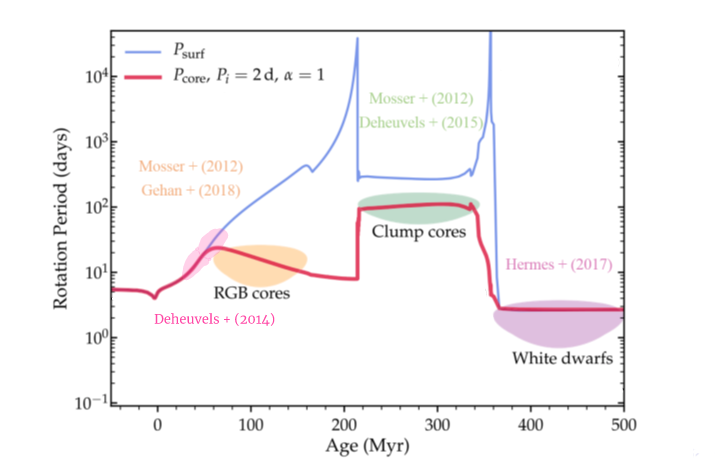
\includegraphics[width=\textwidth]{Figures/intro_figures/qualitative_evo.png}
    \caption{Core (red) and surface (blue) rotation rates with additional angular momentum transport following the prescription of \citet{spada_angular_2016}. Coloured sections denote evolutionary milestones and the works that have provided constraints to these milestones. \textbf{Pink:} subgiant core and surface rotation, \textbf{Orange:} red giant branch cores, \textbf{Green:} clump core rotation rates, and \textbf{Purple:} white dwarf rotation rates. Adapted from Figure 3 in \citet{fuller_slowing_2019}}
    \label{fig:poms_evo}
\end{figure}


Measuring the core and the surface rotation rates of post-main-sequence stars allows us to place constraints on the radial differential rotation of stellar interiors and quantitatively probe the evolution of angular momentum transport.
Observations of young subgiants suggest that terminal age main sequence stars' rotation profiles are relatively flat \citep{deheuvels_seismic_2020}.
However, observations of older post-main-sequence stars have raised more questions than they have answered \citep{beck_fast_2012}.
To summarise: angular momentum transport during the post-main-sequence must be greater than state-of-the-art models currently predict.

\citet{deheuvels_seismic_2014} measured the core and surface rotation rates of 6 subgiants/young red giants.
The observed core to surface rotation ratio of subgiants and the core rotation rates of red giant branch stars suggest that additional angular momentum transport is unaccounted for in state-of-the-art models of rotating stellar evolution \citep{deheuvels_seismic_2014, spada_angular_2016, moyano_asteroseismology_2022}.
The scale of the core-to-surface rotation rate ratio of subgiants ($\Omega_c/\Omega_s$) is one to two orders of magnitude smaller than models predict \citep{fuller_asteroseismology_2015,spada_angular_2016,ouazzani_gamma_2018, eggenberger_asteroseismology_2019}.
While core rotation rates were first believed to decrease along the red giant branch\footnote{Indeed when core rotation rates of red giants are plotted against $\log{g}$, a proxy for evolution, they do appear to decrease with evolution. When plotted against the more appropriate scale of mixed mode coupling (See Equation 10 in \citet{gehan_core_2018} and compare Figures 12 and 13 in this work), they are constant with evolution.} \citep{mosser_spin_2012} revised measurements and a larger sample size revealed that the core rotation rates of red giant branch stars appear constant with evolution when the contraction of the core should spin them up.
\citep{mosser_spin_2012,gehan_core_2018,moyano_asteroseismology_2022}.
The core rotation rates of early red giant branch and red clump stars suggest a continued excess angular momentum transport during this phase of evolution \citep{cantiello_angular_2014,moyano_asteroseismology_2022}.
On the other hand, observed white dwarf rotation rates can be recovered from the observed core rotation of clump stars assuming conservation of angular momentum. \citep{cantiello_angular_2014, den_hartogh_constraining_2019}
\citet{cantiello_angular_2014} suggests that this feature may be owing to the short evolutionary timescale between the red clump and white dwarf phases rather than indicative of a decrease in the excess angular momentum transport.


The physical mechanism underlying the excess angular momentum transport is currently unidentified.
Several notable relations with mass and evolutionary state have been determined by calculating the excess angular momentum transport required to match observations. 
\citet{spada_angular_2016} quantified the increased angular momentum transport required to match the observed subgiant core and surface rotation rates measured in \citet{deheuvels_seismic_2014}.
They introduced an additive angular momentum diffusion coefficient to the transport of angular momentum equation in the radiative zone, which obeys an advection-diffusion equation: 
\begin{equation}
    \rho \frac{\text{d}}{\text{dt}}\left(r^2 \Omega \left( r \right)\right) = \frac{1}{5r^2}\frac{\partial}{\partial r}\left(\rho r^4 \Omega \left( r \right)
 \ U\left(r\right)\right) + \frac{1}{r^2}\frac{\partial}{\partial r} \left(\rho \left( D_{\text{shear}} + v_{\text{add}}\right) r^4 \frac{\partial \Omega\left( r \right)}{\partial r}\right),
\end{equation}
\citep{zahn_circulation_1992,maeder_stellar_1998,eggenberger_geneva_2008}
where $r$ and $\rho$ are the characteristic radius and density on an isobar. $\Omega(r)$ is the mean rotational rate and $U(r)$ is the velocity of meridional currents in the radial direction. $D_{\text{shear}}$ is the diffusion coefficient for the angular momentum shear instability (See Equation 10 in \citet{eggenberger_effects_2010}) and $v_{\text{add}}$ is the additional viscosity corresponding to the excess angular momentum transport.
Their results suggest that the additional angular momentum transport decreases as stars ascend the subgiant branch and increases with mass.
The suggested scale of excess angular momentum transport they propose is on the order of $10^3-10^4 \text{cm}^2 \text{s}^{-1}$.
Which is similar to $D_{\text{shear}}$ close to the convective envelope but rapidly decreases to the order of $10^1\text{cm}^2 \text{s}^{-1}$ in the stellar core.
Comparing Figures \ref{fig:deh_without} and \ref{fig:deh_with} we see that the introduction of the additional viscosity to the model term results agreement with the core to surface rotation fraction in the \citet{deheuvels_seismic_2014} sample.

\citet{moyano_asteroseismology_2022} performed a similar analysis but with the core rotation rates of red giant branch and red clump stars measured in \citep{mosser_spin_2012} and \citet{gehan_core_2018}.
They found that the same order of magnitude additional viscosity term was required to explain the approximately constant core rotation rates of red giant and red clump stars.  
Qualitatively they found that the additional angular momentum transport becomes stronger when the star evolves up the red giant branch through shell hydrogen burning.
Angular momentum must be redistributed between two to three orders of
magnitude more efficiently for red clump stars than for red giants closer to the main-sequence turn-off consistent with \citet{den_hartogh_constraining_2019}.
Figures \ref{fig:rgb_cores_without} and \ref{fig:deh_with} highlight that models of red-giant evolution with the additional viscosity introduced in this work now agree with the observed core rotation rates observed in \citet{gehan_core_2018}.

\begin{figure}[h]
    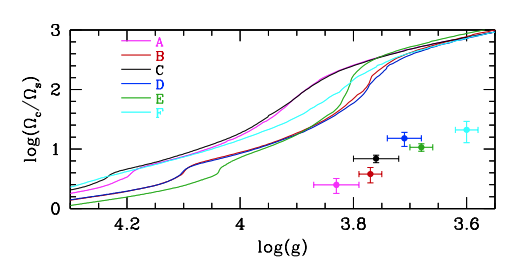
\includegraphics[width=\textwidth]{Figures/intro_figures/deheuvels_disparity_without.png}
    \caption{log of core to surface rotation rate against $\log{g}$. 
    \textbf{Dots:} Observed core to surface rotation rates of the six subgiants measured in the \citet{deheuvels_seismic_2014} sample (A,B,C,D,E,F).
    \textbf{Lines:} rotating models of the stars in that sample without additional angular momentum transport \citep{eggenberger_asteroseismology_2019}.
    The observed core-to-surface rotation rates are much smaller than models predict. This implies additional angular momentum transport than is currently accounted for models.
    Sourced from Figure 2 in \citep{eggenberger_asteroseismology_2019}.}
    \label{fig:deh_without}
\end{figure}

\begin{figure}[h]
    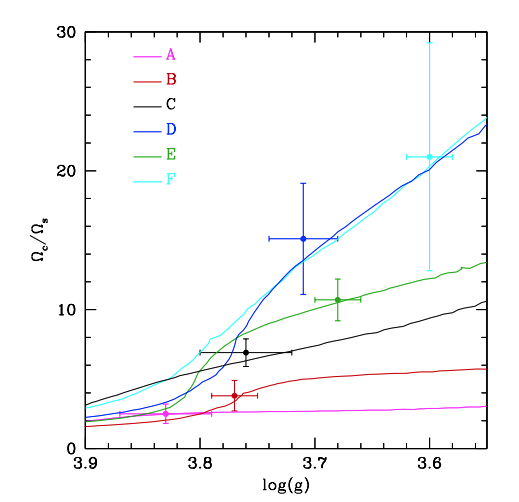
\includegraphics[width=\textwidth]{Figures/intro_figures/deheuvels_disparity_with.png}
    \caption{Same as Figure \ref{fig:deh_without} but with additional angular momentum transport introduced for the models to reflect the observations.
    Sourced from Figure 3 in \citep{eggenberger_asteroseismology_2019}.}
    \label{fig:deh_with}
\end{figure}


\begin{figure}[h]
    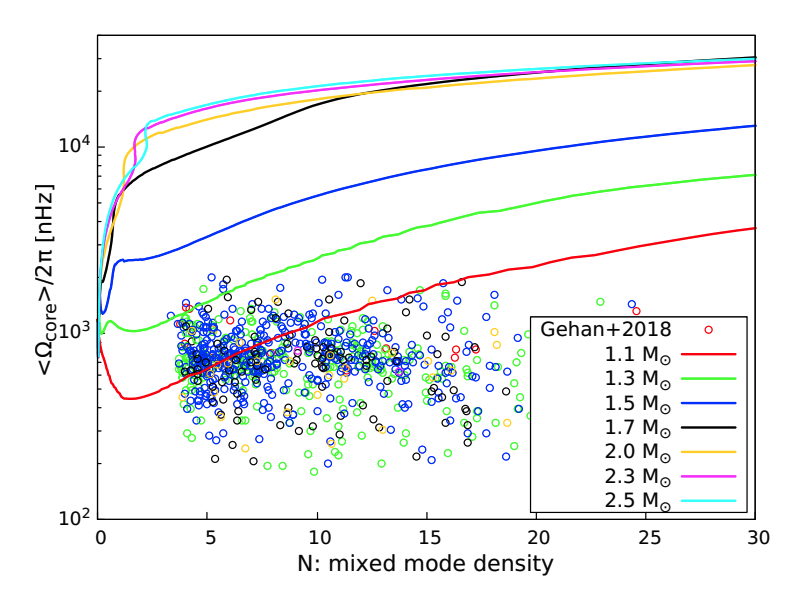
\includegraphics[width=\textwidth]{Figures/intro_figures/rgb_core_rot_without.png}
    \caption{Average core rotation rates of red giants against mixed mode density (a proxy for evolution) 
    \textbf{Dots:} Observed core rotation rates from \citet{gehan_core_2018}
    \textbf{Lines:} rotating models of the stars in that sample without additional angular momentum transport \citep{moyano_asteroseismology_2022}.
    The observed core rates are much smaller than models predict. Implying excess angular momentum transport is required for the models to reflect the observations.
    Sourced from Figure 6 in \citep{moyano_asteroseismology_2022}.}
    \label{fig:rgb_cores_without}
\end{figure}

\begin{figure}[h]
    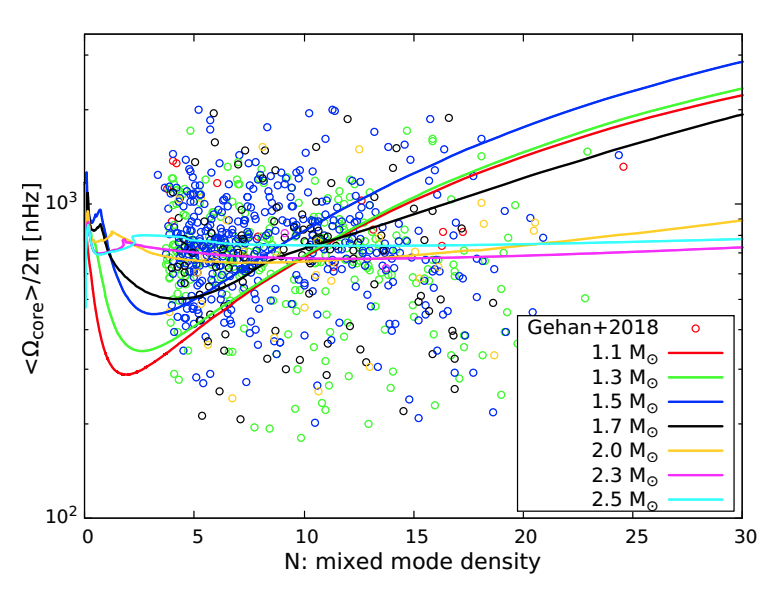
\includegraphics[width=\textwidth]{Figures/intro_figures/rgb_core_rot.png}
    \caption{Same as Figure \ref{fig:rgb_cores_without} but with additional angular momentum transport introduced for the models to reflect the observations.
    Sourced from Figure 7 in \citep{moyano_asteroseismology_2022}.}
    \label{fig:rgb_cores_with}
\end{figure}


Several modes of excess angular momentum transport have been suggested to explain the disparity between models and observations.
\citet{barker_angular_2019,barker_angular_2020} studied the role of
the Goldreich-Schuber-Fricke (GSF) instability (\citep{goldreich_differential_1967,fricke_rotation_1967} and its role in angular momentum transport for post-main-sequence stars.
They suggest that the GSF instability can introduce additional viscosity up to $10^4 \text{cm}^2 \text{s}^{-1}$ for low-mass stars but is two orders of magnitude too small to reflect the rotation of higher mass stars not discussed in this work.

Magnetorotational instabilities constitute another candidate to explain the internal rotation of evolved stars.
Two potential candidates are azimuthal magnetic rotational instabilities (AMRI) \citep{ruediger_astrophysical_2014,rudiger_diffusive_2015} and the Tayler-Spruit instability \citep{spruit_dynamo_2002} (See Section \ref{sec:magneto_rotational_instabilities}).
\citet{rudiger_diffusive_2015} suggest AMRIs can increase molecular viscosity to the magnitude required to explain observations.
On the other hand, there is no evidence to suggest that this instability reflects the trends with mass and evolution.
The Tayler instability does introduce excess angular momentum transport in the post-main-sequence \citep{fuller_slowing_2019}, however, it cannot simultaneously reflect the observations of both subgiants and red giants \citep{eggenberger_asteroseismology_2019,den_hartogh_constraining_2019}.


\citet{spada_angular_2016} propose the efficiency of angular momentum transport may be related to the core to surface rotation rate to some power - $\left(\Omega_c/\Omega_s\right)^{\alpha}$ - which can be related to magnetorotational instabilities.
This work suggests that $\alpha = 3$ reflects the core rotation rates of red giants claimed in \citep{mosser_spin_2012}.
\citet{moyano_asteroseismology_2022} revisited this prescription and found that $alpha = 3$ more accurately reflects the approximately constant rotation core rotation rates of red giants observed by \citet{gehan_core_2018}.
\citet{spada_angular_2016} was limited to a single model with mass = 1.25 $M_{\odot}$.
No parameterisation with mass was therefore performed.

Other physical mechanisms have been suggested to have a role in excess angular momentum transport, such as angular momentum transport by internal gravity waves \citep{pincon_can_2017} or mixed-modes \citep{belkacem_angular_2015}. 
However, the scale of their introduced additional viscosity is yet to be investigated.
Disentangling each of these proposed mechanisms' relative importance to the additional angular momentum transport required to explain the observations requires much more data.


%On the other hand the subgiant phase is short-lived and steroseismic inference of the rotation profile is data-intensive in that it requires short-cadence observations of stars over long observation periods for high enough SNR to measure rotational splittings.
%As a result, only ~30 subgiant and young red giants that exhibit oscillation modes that probe both the core and the surface have been asteroseismically probed.

We speculate that the simultaneous measurement of subgiants' core and surface rotation rates may be the best probes for constraining the excess angular momentum transport.
A few pathways exist to further probe the mechanism underlying excess angular momentum transport through asteroseismology alone.
Either: a) more stars need to have their core and surface rotation rates measured through asteroseismology (which we will denote ensemble fitting), or b) stronger constraints must be placed on the rotation profile between the core and the surface (single star constraints).

On the former, if more stars have their core and surface rotation rates observed, then more measurements of the excess angular momentum transport required for state-of-the-art models to match the observations are made.
The excess angular momentum transport required to match observations appears mass and evolutionary-dependent.
Stronger constraints to the dependency of the excess angular momentum transport on these quantities provide information about the underlying mechanism.
The Kepler asteroseismic data currently available suggests that the efficiency of the excess angular momentum transport increases with the star's mass \citep{eggenberger_asteroseismology_2019}.
However, the efficiency of angular momentum transport decreases with evolution during the subgiant phase.
Consequently, a transport process with efficiency dependent on the angular momentum gradient between the core and the surface cannot be at play in subgiants.
Identifying with more precision the dependency of excess angular momentum transport on stellar quantities would provide evidence for or discredit proposed mechanisms.

On the latter, the internal shape of the rotation profile of subgiants reflects the underlying mechanism that created it.
Therefore, evidence for or against particular shape of rotation profiles is illuminating to proposed mechanisms.
A strong gradient in the rotation profile in the core of a subgiant, for example, is incompatible with angular momentum transport through deep fossil magnetic fields \citep{gough_effect_1990} as they would likely smooth out sharp features.
 This is because differential rotation is expected to be damped along poloidal field lines (\citealp{garaud_rotationally_2002, strugarek_magnetic_2011}).
 Internal gravity waves, on the other hand, are expected to be efficient during the advanced phases of stellar evolution \citep{charbonnel_deep_2008}. 
Internal gravity waves can give birth to localised weak gradients in the rotation profile as a result of extraction and deposit of angular momentum \citep{charbonnel_influence_2005}. 
A sharp rotational gradient could also potentially trigger magneto-rotational instabilities that would transport angular momentum (\citealp{balbus_stability_1994,arlt_differential_2003,menou_magnetorotational_2006, fuller_asteroseismology_2015, fuller_slowing_2019,moyano_asteroseismology_2022}). 
Evidence of a strong angular momentum gradient towards the core of a sub-giants quickly constrains the number of possible angular momentum transport mechanisms to solve the angular momentum transport problem.

Two obvious problems impede the single-star pathway. 
These are the need for observations of high SNR higher degree modes and the results of methods used to measure rotation profiles being unstable to high-resolution inversions. 
Constraints on the rotation profile in intermediate points between the core and surface require the observations of oscillation modes of $l \approx 10$ \citep{ahlborn_asteroseismic_2020}. 
For reliable measurements of such oscillations, much longer observation periods, longer than \corot{} and \kepler{}, of sub-giants are required.
   
Both of these pathways require much more asteroseismic data than is currently available.
For ensemble fitting to be viable many subgiants would need to be observed over long baselines with short cadence observations.
If the Kepler mission is exemplary, then the baseline required for high-SNR asteroseismic observations is on the order of ~4 years per star.

At the time of writing, ~30 subgiants show evidence of rotational splittings \citep{li_asteroseismology_2020,li_asteroseismology_2020-1}, though the rotational splitting data is yet to be released and analysed.
The results will be undoubtedly informative, though we will not speculate exactly how much they will solve the subgiant excess angular momentum transport problem.
\citet{hatt_catalogue_2023} suggests that there is $\sim$4000 stars in the TESS - short cadence catalogue with observable solar-like oscillation features.
The measured frequency of peak oscillation power $\nu_{\text{max}}$ of stars in these sample suggests that some of these stars are subgiants.
While no rotational splittings of these stars have been reported some of these stars may lay in the continuous viewing zone.
This means their observation periods are approaching 4 years at time of writing and these stars may soon offer a seperate sample of subgiants with observations of asteroseismic rotational splittings.
While we may speculate about future asteroseismic focussed missions, it will be some time before any new asteroseismic rotation signals in subgiants are made.

Independent constraints can also be placed on the evolution of the surface rotation of subgiants.
\citet{santos_surface_2021} measured the surface rotation of 4500 subgiants using photometric oscillations from stellar spots.
The measured rotational periods against their effective temperature are shown in Figure \ref{fig:subgiant_surface}.
Within this Figure, there are a few notable features.
While subgiants are definitionally older than their main-sequence counterparts, there is a sample of fast-rotating stars coincident with the fast rotators on the main sequence.
This could be explained by most of the stars in this sample being a higher mass than the Kraft break.
They have passed through the main sequence with fast rotating surfaces, entering the subgiant phase; their effective temperatures decrease and are shifted to the right in this diagram relative to their main-sequence counterparts.
The high density of fast-rotating stars could also result from an observational bias.
Long rotational periods require longer baselines to recover and thus have a decreased observed fraction.
Among the sample is a group of slow-rotating (Period $>$ 60 days) targets with Teff between 5000 and 6000 K.
These are consistent with more evolved subgiants as the slowest of these targets are located close to the red giant branch.
This work also suggests that the decreased observation of rotation periods $>$60 days, the strong upper edge of the \citet{mcquillan_rotation_2014} rotational period distribution, is the result of a lack of observations of main-sequence stars rather than an inherent lack of long period probing power by \kepler. 
Whether the upper edge results from angular momentum transport or decreased photometric variability is unknown.
The final feature that is not commented on in their work is an apparent dearth of observations coincident with the intermediate period gap.
Whether this is real or a result of noise is an interesting avenue of research in further understanding the underlying mechanism of the intermediate period gap for main sequence stars.

\begin{figure}[h]
    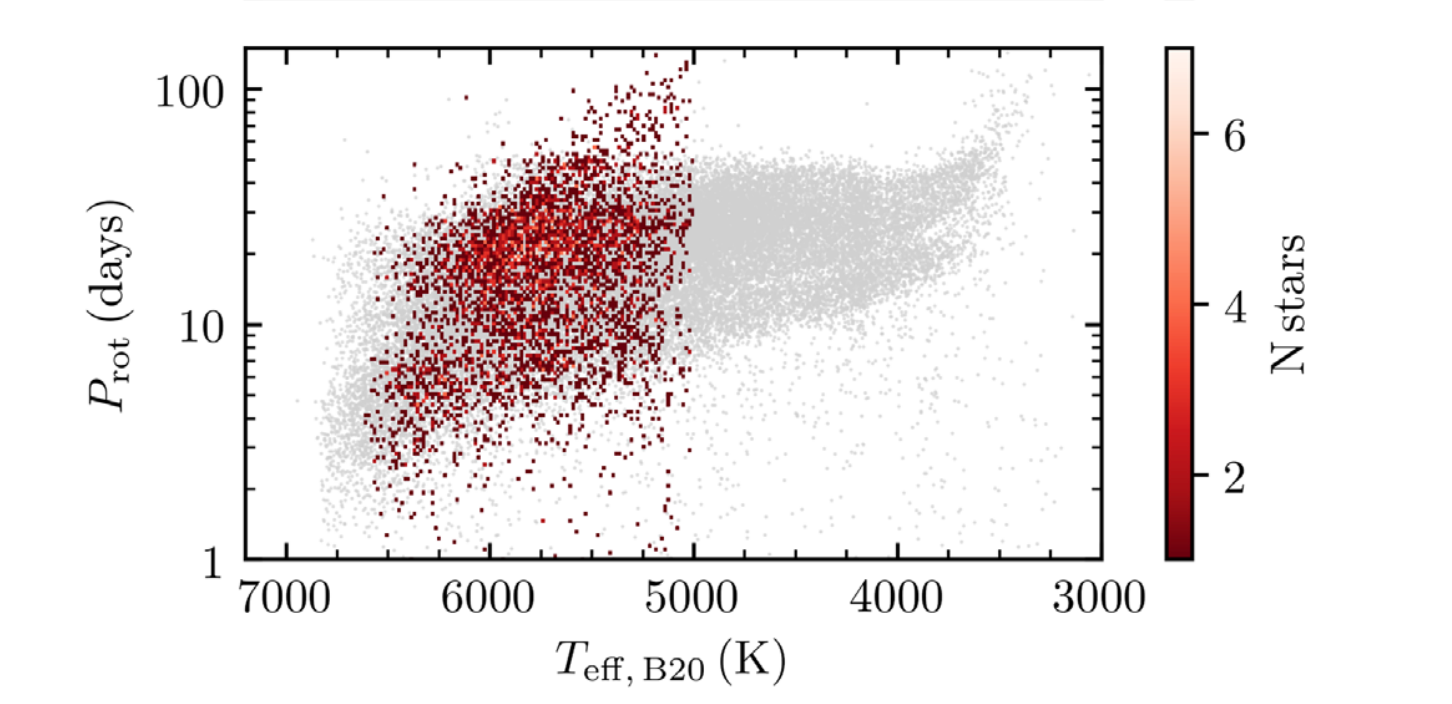
\includegraphics[width=\textwidth]{Figures/intro_figures/subgiant_surface.png}
    \caption{Surface rotation period against effective temperature of subgiants in the \citet{santos_surface_2021} sample overlayed over the \kepler{} \citet{mcquillan_rotation_2014} sample. 
    Sourced from the bottom panel of Figure 5 in \citep{santos_surface_2021}.}
    \label{fig:subgiant_surface}
\end{figure}

\citet{ceillier_surface_2017} measured the surface rotation periods of 361 red giants from stellar spot photometric variability.
The measured rotational periods against their mass are shown in Figure \ref{fig:rgb_surface}.
Expectedly, comparative to the subgiant analysis of \citet{santos_surface_2021} the surface rotation period of red giant stars is greater than their subgiant counterparts.
They suggest that the surfaces of these stars rotate faster than models suggest \citep{tayar_rapid_2015}.
They conclude that the large percentage of rapid rotators must result from interactions of red giants with other bodies.
This work, however, is older than the revised excess angular momentum transport research discussed earlier in this work.
Their results need to be reexamined within the context of excess angular momentum transport.

\begin{figure}[h]
    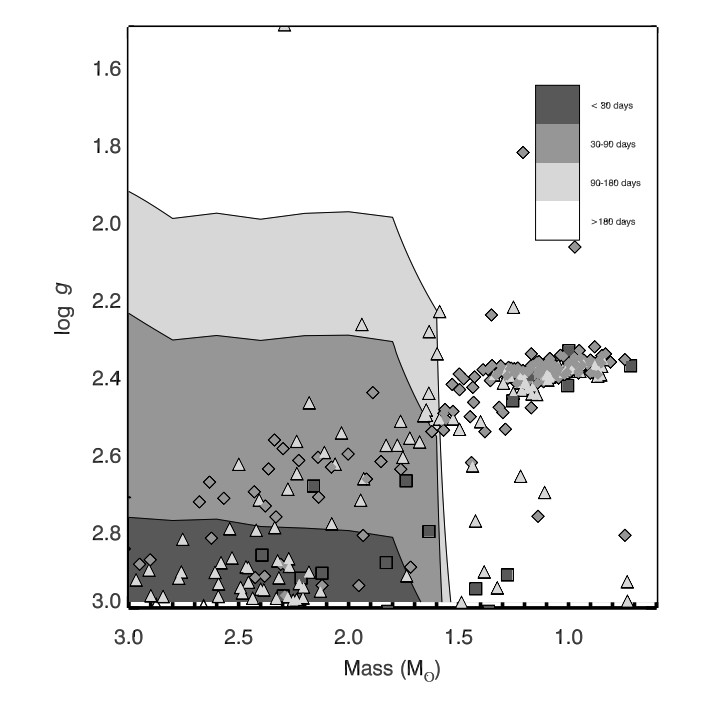
\includegraphics[width=\textwidth]{Figures/intro_figures/rgb_surface.png}
    \caption{Surface rotation period against mass of red giant stars from \citet{ceillier_surface_2017}.
    Sourced from the top panel of Figure 7 in \citep{ceillier_surface_2017}.}
    \label{fig:rgb_surface}
\end{figure}

Finally, we discuss the rotating remnants of low-mass post-main-sequence evolution: white dwarfs.
White dwarfs do not evolve rotationally, though their observed rotation rates constrain angular momentum during the red clump phase.
\citet{hermes_white_2017} suggest that the rotation periods of white dwarfs decrease with the progenitor's mass.
As previously discussed, the surface rotation rates of white dwarfs are consistent with angular momentum conservation following the red clump \citep{den_hartogh_constraining_2019, cantiello_angular_2014}.
This is because the time scale of angular momentum transport is longer than the timescale of evolution from red clump star to a white dwarf.
\citet{den_hartogh_constraining_2019} suggest that mass-dependent angular momentum transport must decrease with evolution along the red clump such that the angular momentum of terminal red clump rotation cores agree with the angular momentum of white dwarf stars.

\section{Effects of rotation}
\label{sec:effects}

Within the previous Section, we discussed the evolution of rotation from birth to remnants of evolution.
While we now have an understanding of this evolution, we still need to clarify the effects of rotation on stellar evolution.

\subsection{Hydrostatic effects}

The effects of rotation on stellar evolution are varied and complex.
In general, the hydrostatic effects of rotation have only minimal effects on the internal evolution of stars \citep{kippenhahn_rotation_1970,maeder_evolution_2000}.
Especially the low-mass, slowly rotating stars we consider in this work.
In this Section, we review how some of these effects are treated in current models of stellar evolution, the resulting changes to stellar evolution brought about by these effects and their observable consequences.
We will begin by discussing the effects of stellar rotation on hydrostatic equilibrium.


As a star rotates, its equilibrium configuration deviates from the non-rotating hydrostatic equilibrium due to centrifugal forces. 
Rotation-induced centrifugal forces induce deviations from spherical symmetry.
Only if the rotation energy of a star approaches a significant fraction of the gravitational potential energy will observable triaxial deformation occurs.
Low-mass stars usually rotate slowly, so these effects are rarely seen.

The four equations of stellar structure need to account for this change to the equilibrium configuration.
\citet{kippenhahn_simple_1970} devised the method to account for this where a conservative potential exists.
In this method, they replace the notion of spherical stratification of non-rotating stars with a rotationally deformed shellular stratification where the structural variables - e.g. pressure ($P$), density ($\rho$), temperature ($T$), chemical abundances - are constant on an equipotential.
The equipotential in this prescription is defined as 
$\Psi = \Phi + \frac{1}{2}\Omega^2 r^2 \sin^2 \theta$, the non-rotating gravitational potential modulated by the centrifugal force, where $Phi$ is the gravitational potential, $\theta$ the latitude relative to the rotational axis and $\Omega$ the angular rotation rate.
This method applies only when a conservative potential exists, i.e. when the angular velocity distribution is cylindrically symmetric \citep{tassoul_theory_1978}.
The internal rotation generally evolves towards rotation laws that are non-conservative.
For example, \citet{zahn_circulation_1992} suggests that turbulence is anisotropic, with a stronger transport horizontally than vertically. 
This results in a constant rotation rate on isobars and does not fall into the conservative case.
\citet{maeder_diffusive_1996} revise \citet{kippenhahn_circulation_1974}'s method and prescribe a consistent description of shellular rotation on isobars which is valid for slow rotation.
On these isobars, the non-rotating stellar variables and angular momentum are constant. 
This allows models of rotating stellar evolution to be kept one-dimensional.

The equations of stellar structure are mainly affected by rotation through a few key concepts.
Centrifugal forces reduce effective gravity for all points in the star that are not on the axis of rotation.
The centrifugal forces vary with radial distance and latitude, resulting in equipotentials closer together along the rotational axis than the equatorial axis.
Radiative flux varies with local effective gravity \citep{von_zeipel_radiative_1924}.
This results in gravitational darkening \citep{von_zeipel_radiative_1924, kippenhahn_rotational_1977} - stars are higher temperature and have larger temperature and radiation flux along the rotational axis compared to the equatorial axis.
Gravity darkening of slowly rotating stars (rotation rates much slower than the break-up velocity like those considered in this work) is very small - $<<$0.1\% variation in luminosity and temperature across their surfaces.
Stars close to critical rotation rate should be treated with care \citep{kippenhahn_rotational_1977,maeder_stellar_1999,heger_presupernova_2000}.

\subsection{Increased mixing in stars}

Rotation can extend the mixing regions in stars - allowing mixing between the radiative core and convective envelope - and increase the mixing efficiency through meridional circulation and rotational instabilities.

For convenience, throughout the following Section, we make use of the following gradients:
\begin{equation}
    \nabla_{\textnormal{ad}} := \left(\frac{\partial \ln T}{\partial \ln P}\right)_{\textnormal{ad}}, \ \  \nabla_{\mu} := \frac{\der \ln \mu}{ \der \ln P}, \ \ \nabla := \frac{\der \ln T}{\der \ln P}
\end{equation}
\begin{equation}
    \delta := -\left(\frac{\partial\ln \rho}{\partial \ln T}\right)_{\mu,P}, \ \  \varphi := \left(\frac{\partial \ln \rho}{\partial \ln \mu}\right)_{P,T},
\end{equation}
where $\mu$ is the mean molecular weight at a given position in a star. The subscript "ad" refers to the gradient if we adiabatically transported a fluid element along a path.
$\nabla$ is simply the temperature gradient relative to the pressure gradient, $\nabla_{\textnormal{ad}}$ is our temperature gradient relative to the pressure gradient along an adiabat, that is, the temperature gradient that arises from adiabatically transporting fluid elements along $P$, $\nabla_{\mu}$ is the composition gradient with relative to the changing pressure, $\delta$ is the density gradient relative to the temperature along paths of constant $\mu$ and $P$ and $\varphi$ is the density gradient relative to the mean molecular weight along paths of constant $P$ and $T$.

In non-rotating stars, mixing can be simplified by whether a region in a star is convective, semi-convective, radiative or undergoing thermohaline mixing \citep[These concepts will not be discussed at length in this work. See][ for good overviews of these concepts.]{maeder_evolution_2000,tassoul_stellar_2000}
Convective regions are well mixed and have no chemical gradients, as convection acts on local dynamical time scales, while radiative regions are not well mixed and are generally chemically stratified.
Semi-convective regions are thermally unstable regions stabilised against convection by a gradient in composition.
Thermohaline mixing arises when an unstable gradient in composition (mean molecular weight) is only partially stabilised by thermal stability.
Semi-convection and thermohaline mixing act on longer time scales than convection; their effective diffusion coefficient is smaller.
The conditions required for semi-convection and thermohaline mixing are well discussed in the works referenced above.
Here we will focus on convective and radiative regions for simplicity.
Whether a region is convective or radiative is defined by whether the Brunt-V\"{a}is\"{a}l\"{a} frequency, the characteristic oscillation frequency of a displaced particle of fluid in a stratified density medium is positive or negative.
\begin{equation}
    N^2 = \frac{g \delta}{H_\textnormal{P}}\left(\nabla_{\textnormal{ad}} - \nabla + \frac{\varphi}{\delta} \nabla_{\mu}\right), 
\end{equation}
where $H_P$ is the local pressure scale height ( $H_{P
} = \frac{P}{\rho g}$ in hydrostatic equillibrium, where $P$ is local pressure, $\rho$ is local density and $g$ local effective gravity).
Rotation can overcome the pressure, density and mean molecular weight gradients to push mixing into previously stable regions through rotational instabilities.

When we discuss the Brunt-V\"{a}is\"{a}l\"{a} frequency, it is worth thinking of the characteristic oscillations of mass parcels.
When the Brunt-V\"{a}is\"{a}l\"{a} frequency is negative, the oscillations grow exponentially, leading to enhanced mixing.
The mixing process is treated as essentially instantaneous in models.
When it is positive, the oscillations are bounded, and mixing does not occur.
On the other hand, when the Brunt-V\"{a}is\"{a}l\"{a} frequency is negative but very close to zero, the oscillations grow slower than in the case of convection.
While some instabilities act on dynamical time scales, we do not treat diffusion due to instabilities as if they were convective.
In that way, we separate the effect of instabilities by their contribution to the total effective diffusion at every point in a star.

Here we will briefly discuss a non-exhaustive list of rotational instabilities and how they impact the mixing of stars.
Most of these instabilities are not expected to arise during the low-mass ($<$8$M_{sol}$) main-sequence evolution due to the small angular momentum gradients of main-sequence stars, as discussed in the previous Section.
However, they are influential during evolutionary periods where strong rotational gradients arise: during the post-main-sequence or core envelope decoupling as suggested in some models of young-main sequence evolution \citep{heger_presupernova_2000}.


We separate the instabilities by the timescale. 
They act upon dynamic and secular instabilities.
We expect secular instabilities to act on during the main sequence when rotational gradients are small and evolutionary times scales are long.
On the other hand, strong rotational gradients arise during the post-main-sequence.
Dynamical instabilities also act on shorter timescales than evolutionary timescales in the post-main-sequence
As a result, dynamical instabilities are mainly expected to play a role during the post-main-sequence.

\subsubsection{Dynamical shear instability}

The dynamical shear instability arises when the energy that can be gained from a shear flow (a rotational gradient) is comparable to the work that must be done to displace a mass element adiabatically. 
This means the instability is inhibited by density gradients but is very effective along isobars \citep{endal_evolution_1978,pinsonneault_evolutionary_1989,heger_presupernova_1998}, supporting the shellular isobaric representation of rotation in stellar models.

The condition for stability is dependent on the local rotational gradient modulating the Brunt-V\"{a}is\"{a}l\"{a} frequency:
\begin{equation}
    Ri = \frac{g \delta}{H_P}\left(\nabla_{\textnormal{ad}} - \nabla + \frac{\varphi}{\delta}\nabla_{\mu}\right)\left(g \frac{d \ln r}{d \Omega}\right)^2 > Ri_C,
    \label{eqn:richoooo}
\end{equation}
where $\omega$ is the angular rotation rate and $Ri_C$ is the critical Richardson number = 1/4 \citep{zahn_rotational_1974}. 
The region is considered stable if $Ri>Ri_C$, and the diffusion coefficient is 0.
When unstable, the diffusion coefficient is proportional to the extent to which the rotational gradient overcomes the chemical and temperature gradients, $Ri/Ri_C$, the spatial extent of the unstable region, and the local dynamical timescale.

\subsubsection{Solberg-H\o iland instability}

The Solberg-H\o iland instability occurs when introducing the centrifugal force to the net force on an adiabatically displaced mass element overcomes the thermal and chemical gradient stabilities.
The condition for stability is given by:
\begin{equation}
    R_{SH} = \frac{g \delta}{H_P}\left[ \nabla_{ad} - \nabla + \frac{\varphi}{\delta} \nabla_{\mu} \right] + \frac{1}{r^3}\frac{\der}{\der r}\left(r^2\Omega\right)^2\geq 0,
\end{equation}
The second term in the equation accounts for the introduction of rotation, where the specific angular momentum ($j$) is $r^2\Omega$ \citep{tassoul_theory_1978,kippenhahn_stellar_1990,heger_presupernova_2000}. 
Under no rotation (or no angular momentum gradient), we recover the Brunt-V\"{a}is\"{a}l\"{a} frequency.

For the Solberg-H\o iland instability to occur, the second term in the equation must be negative and, therefore, only occurs in regions of decreasing angular momentum (a negative rotation gradient with respect to radius).
The diffusion coefficient associated with this instability increases with $R_{SH}$ - the more the angular momentum gradient overcomes the thermal stability, the greater the mixing effect -the spatial extent of the unstable region, the local dynamical timescale.

\subsubsection{Secular shear instability}

When thermal dissipation is significant, the restoring force of buoyancy is reduced, and the strict criteria for the dynamical shear instability to act can be relaxed.
Due to this process requiring thermal dissipation, it operates on the relatively slower (secular) thermal-time scale, hence its name.

\citet{endal_evolution_1978} suggest two stability conditions against secular shear instability. The first is a modulation to the thermal stability component of the Brunt-V\"{a}is\"{a}l\"{a} frequency by a product of the Reynolds number - a dimensionless fluid flow number - and Prandtl number ($P_E$):
\begin{equation}
    R_{is,1} = P_E \frac{g \delta}{H_P}\left(\nabla_{\textnormal{ad}} - \nabla \right)\left(g \frac{\der \ln r}{\der \Omega}\right)^2 > Ri_C,
    \label{eq:ssi1}
\end{equation}
where $P_E = \frac{P_r R_{e,c}}{8}$. $R_{e,c}$ is the critical Reynolds number of the flow of material, and $Pr$ is the Prandtl number, the ratio of the thermal diffusion timescale to the angular momentum diffusion timescale \citep[See][and references therein for a more thorough explanation of these quantities and their implementation in models of stellar rotation]{tassoul_theory_1978,heger_presupernova_1998}.

The second condition is the mean molecular weight component of the dynamical shear instability, which is not affected by the relaxation of thermal adjustment
\begin{equation}
    R_{is,2} = \nabla_{\mu} \frac{g \varphi}{H_P}\left(g \frac{\der \ln r}{\der \Omega}\right)^2 > Ri_C.
\end{equation}
The need for the inclusion of this term is debated, however.

\citet{endal_evolution_1978} suggest that the diffusion coefficient scales with the characteristic velocity of the secular shear instability, the characteristic scale height - the combination of which provides the characteristic timescale - and either $R_{is,1}$ and $R_{is,2}$ whichever violates the criteria more.

Many works have shown that the molecular gradient inhibits mixing by up two orders of magnitude than observations suggest.
Those who include the term include a factor on $\nabla_{\mu}$ of order $<$0.05 to account for this \citep{charbonnel_lithium_1994,heger_presupernova_2000}.

\citet{maeder_stellar_1997} argues that the regions where molecular gradients are strong enough to inhibit mixing from the secular shear instability, near the core, are generally semi-convective and experience some mixing/turbulence already.
They suggest that in a semi-convection region (or in any zone with other sources of turbulence), some fraction of the local energy excess in the shear is degraded by turbulence to change the local entropy gradient. 
They hypothesise that this turbulence will affect the shear energy and molecular gradient and calculate a diffusion coefficient under this assumption. 
They find that the diffusion coefficient is consistent with the semi-convective diffusion coefficient when turbulence overcomes the shear and towards $K/R_{is,1}$ when semi-convection is negligible \citep[Consistent with the results of][]{zahn_circulation_1992}.
\citet{talon_anisotropic_1997}, on the other hand, account for the mixing effect of horizontal diffusion from semi-convection on the restoring force produced by the molecular gradient, which reduces its stabilising effect.
Both works result in the diffusion of elements consistent with observations without adding new factors.



\subsubsection{Meridional circulation}
Meridional circulation \citep{eddington_circulating_1925} arises from gravity darkening.
Excess flux along the rotational axis heats material more than along the equator.
This drives the large-scale circulation of material from the pole to the equator.
This results in angular momentum transport and chemical transport.
Early theoretical considerations of meridional circulation were not physically consistent.
They predict inverse circulation (from the equator to the axis of rotation) close to the surface, and they did not conserve angular momentum \citep{sweet_importance_1950, mestel_rotation_1953, mestel_star_1956, kippenhahn_stellar_1990}.

Meridional circulation can be treated differently for the transport of elements and the transport of angular momentum.
\citet{endal_evolution_1978} derived a
In this prescription, the diffusion coefficient scales with the Eddington-Sweet velocity and the extent of the region where the process is in effect \citep[See][]{kippenhahn_circulation_1974, endal_evolution_1978,heger_presupernova_2000}.

On the other hand, \citet{zahn_circulation_1992} determined that energy conservation, gravity and angular momentum much be calculated simultaneously for a self-consistent and physically possible solution to be found.
\citet{chaboyer_effect_1992} showed that if the horizontal component of turbulence is large, the effects of meridional circulation on the transport of elements is equivalent to a diffusion process with diffusion coefficient $D_{\text{mr}}$.
\begin{equation}
    D_{\text{mr}} = \frac{\left| r U(r)\right|^2}{30 D_h}
    \label{eq:mr_d}
\end{equation}
$D_h$ is the coefficient of horizontal turbulence, $U(r)$ is the vertical component of the meridional circulation velocity, and $r$ is the radius at which the components are calculated.
While diffusion from horizontal turbulence is required for meridional circulation to be treated as a diffusive process, it is also inhibited.

Measurements of the Lithium-7 abundance in the sun support this prescription.
The difference between the derived diffusion coefficients from \citet{kippenhahn_circulation_1974,endal_evolution_1978, heger_presupernova_2000} and \citet{chaboyer_effect_1992} prescriptions is approximately a factor of 30 scaling.
\citet{pinsonneault_evolutionary_1989} found that a scaling of 0.046 ($\sim$ 1/30) of the \citet{kippenhahn_circulation_1974} diffusion coefficient is required to reproduce the observed Lithium-7 abundances.
Indeed the two prescriptions are appropriate with sufficient scaling.

Prescriptions for horizontal diffusivity ($D_h$) are lacking in physical motivation.
\citet{zahn_circulation_1992} suggests  $\left|rU(r)\right|$ is an adequate prescription.
\citet{maeder_stellar_2003} derived an expression with respect to energy considerations, while \citet{mathis_transport_2004} adapted a prescription from laboratory experiments.
\citet{mathis_anisotropic_2018} suggest that the anisotropy of turbulent transport scales as  $N^4\tau^2/(2\omega^2)$ , where $N$ and $\omega$ are the Brunt-V\"{a}is\"{a}l\"{a} and rotation frequencies and $\tau$ the time scale characterising the source of the turbulence.  
Their results all generally agree though this does not suggest that they are the correct formalisation of horizontal diffusion.

Angular momentum transport by meridional circulation can be treated as an advective or diffusive process.
Consider the path of a fluid element along a meridional eddy.
Meridional circulation describes a rise of material along the rotational axis, descending at the equator.
This results in the transport of angular momentum \textit{against} the angular momentum gradient.
On the other hand, implementing angular momentum transport as a wholely diffusive process is numerically simpler \citep{endal_evolution_1978,pinsonneault_evolutionary_1989,heger_presupernova_2000}.
The two implementations may deviate in regions where meridional circulation dominates.
The two implementations obtain similar results along the main-sequence \citep{talon_anisotropic_1997,heger_presupernova_2000} where the evolutionary timescale is long enough for meridional circulation to be impactful.

\citet{zahn_circulation_1992} derived the radial component of the velocity of meridional circulation ($U(r)$) under the effects of thermal and molecular weight gradients.
\begin{equation}
    U(r) = \frac{1}{H_P C_P T \left[ \nabla_{\text{ad}} - \nabla + \left( \varphi / \delta \right)\nabla_{\mu}\right]} \left( \frac{L}{M} \left(E_{\Omega} + E_{\mu}\right) \right),
    \label{eq:mr_u}
\end{equation}
where $C_P$ is the specific heat and $E_{\Omega}$ and $E_{\mu}$ are terms dependent on up to the third order derivatives of the rotational distribution and molecular mass distribution \citep[See][]{maeder_stellar_1998}.
This prescription for meridional circulation resolves the inverse circulation of earlier prescriptions and conserves angular momentum.

% Meridional circulation acts on the circularisation timescale:
% \begin{equation}
%     t_{\text{circ}} \simeq \frac{R}{U}
% \end{equation}
% where $R$ and $U$ are characteristic radii of circulation and characteristic circulation velocity timescales, respectively.
% The circularisation time scale is on the order of the secular (thermal) timescales discussed in relevance to the secular instabilities.



\subsubsection{Goldreich-Shubert-Fricke instability}

The Goldreich-Shubert-Fricke (GSF) instability arises when a fluid is unstable to axisymmetric displacements \citep{goldreich_differential_1967,fricke_rotation_1967}.
Stars tend to be inviscid, $P_R$ $<<$ 1.
Under this assumption \citet{kippenhahn_rotation_1970} derives two conditions for stability.
The first is the secular analogue of the Solberg-H\o iland condition for stability under the assumption that the stability from the temperature gradient is removed by thermal conduction
\begin{equation}
    \frac{\partial j}{\partial r} \geq 0.
\end{equation}
The second is an analogue to the Taylor-Proudman theorem for slowly rotating incompressible fluid \citet{kippenhahn_circulation_1974,tassoul_theory_1978, heger_presupernova_2000}.
\begin{equation}
    \frac{\partial \Omega}{\partial z} = 0,
\end{equation}
where $z$ is the distance along the rotational axis.
Fluids are well mixed along equipotentials.
As discussed concerning the Von-Zeipal effect, equipotentials are closer along the rotational axis.
Along an equipotential, if the rotation rate gradient is non-zero, then fluid will be mixed along said equipotential until the rotation profile is conservative.
Stability favours uniform rotation on equipotentials, which is incompatible with shellular rotation except under solid-body rotation.
The GSF instability, therefore, tends to enforce uniform rotation on thermal timescales \citep{endal_evolution_1978}.

The GSF instability demands mixing from meridional circulation and thus, like meridional circulation, acts on the circularisation timescale.

\subsection{Magneto-rotational instabilities}
\label{sec:magneto_rotational_instabilities}

The role of magneto-rotational instabilities in the rotation of stars is debated.
In this Section, we will discuss the theory behind a few of these instabilities and their effects in reference to the post-main-sequence rotational evolution.

Models of post-main-sequence rotational evolution with magnetorotational angular momentum transport suggest that the rotational profile of stars that have undergone significant angular momentum transport track include a strong rotational gradient following the H-burning shell \citep{fuller_slowing_2019,moyano_asteroseismology_2022}.

\subsubsection{Tayler instability and the Spruit Dynamo}

The Tayler instability arises from the interaction between rotation and magnetic fields in a conducting fluid. 
If the magnetic field is aligned with the rotation axis, the Coriolis force tends to twist the field lines into a helical shape.
This can lead to a buildup of tension in the field lines, which can trigger a series of instabilities that amplify the magnetic field.
The end result is a complex pattern of magnetic fields that can drive large-scale flows in the fluid.

The Spruit dynamo, on the other hand, arises from the interaction between rotation and shear flows in a rotating fluid \citep{spruit_dynamo_2002}.
A radial gradient in the rotation rate can generate a shearing motion that can stretch and amplify the magnetic field lines.
This process can lead to the buildup of magnetic energy and the generation of large-scale magnetic fields.

Combining these two mechanisms can lead to forming a self-sustaining magnetic dynamo in rotating stars \citep{spruit_differential_1999}. The Tayler instability can amplify the magnetic field on small scales, while the Spruit dynamo can amplify the magnetic field on large scales. The resulting magnetic fields can drive large-scale flows in the fluid, which in turn can modify the rotation rate and generate new instabilities \citep{fuller_asteroseismology_2015,fuller_slowing_2019}

The instability could be effective even if the initial field strength is small \citep{spruit_why_1998}.
Unfortunately, little is known about the initial field's strength and the efficiency of instabilities in amplifying the magnetic field.
\citet{fuller_slowing_2019} suggests that the Tayler-Spruit instability could play a role in the post-main-sequence angular momentum transport problem discussed in Section \ref{sec:evolution}.

\subsubsection{Azimuthal Magnetorotational instability}

The azimuthal magnetorotational instability (AMRI) is a type of instability that can arise in rotating, magnetised plasmas \citep{hollerbach_non-axisymmetric_2010}. 
It is a variation of the more well-known magnetorotational instability (MRI), which occurs when a weak magnetic field is present in a rotating fluid or plasma.

The AMRI occurs when the magnetic field is not aligned with the rotation axis but is instead perpendicular to it. 
This can happen in astrophysical systems where the magnetic field is generated by a dynamo mechanism or is inherited from the system's initial conditions.
In such cases, the AMRI can become the dominant instability, driving large-scale fluid motions and enhancing the transport of angular momentum \citep{mishra_convective_2021,moyano_asteroseismology_2022}.

The basic idea behind the AMRI is that the magnetic field can act as a free energy source that fluid motions can tap. 
If the magnetic field is perpendicular to the rotation axis, it can introduce a new length scale into the system, leading to a wider range of unstable modes. 
This can result in the growth of perturbations not present in the MRI, leading to more complex dynamics.

The AMRI's strength depends on a star's internal degree of differential rotation.
\citet{moyano_asteroseismology_2022} has discussed the role of the AMRI in relation to the post-main-sequence angular momentum transport problem.
They suggest that a consistent prescription of the AMRI dependent on the degree of internal differential rotation could explain the observed core and surface rotation rates of subgiants and red giants that have not reached the red giant bump.

\subsection{Other angular momentum transport mechanisms}

Here we describe other angular momentum transport mechanisms that are not instabilities but may play a role in the evolution of stellar rotation.
 
One of these mechanisms is angular momentum transport by internal gravity waves (IGWs) \citep{pantillon_angular_2007, kim_angular_2000,talon_hydrodynamical_2005, charbonnel_deep_2008}
IGWs are internal propagation waves that can carry angular momentum from the core to the surface of stars.

Buoyancy forces in a stratified fluid drive internal gravity waves. 
In a rotating fluid, these waves can become distorted by the Coriolis force, leading to the angular momentum transfer between different fluid layers. The wave motion can induce a net angular momentum flux, leading to changes in the rotation rate \citep{zahn_differential_1975}.

One key aspect of this theory is the identification of the so-called "critical layers", which are regions where the wave frequency matches the local rotation frequency. These layers can lead to a resonance between the wave and the rotation, leading to enhanced transport of angular momentum \citep{charbonnel_influence_2005}.

The characteristic rotation profile that would suggest IGWs are at play is a strong rotational gradient tracking the H-burning shell \citep{balbus_stability_1994, menou_magnetorotational_2006}.

Another mechanism that may play a role in post-main-sequence angular momentum transport is the transport of material by mixed modes \citep{belkacem_angular_2015}.
Comparative to the main sequence, post-main sequence stars express mixed modes when only pressure (p) waves propagate in the surface (convective) region.
Mixed modes are gravity (g) modes that are usually constrained to the radiative core that have coupled with p modes.

\citet{belkacem_angular_2015} suggests this process can extract angular momentum from the core of subgiants and red giants.

The efficiency of this angular momentum transport mechanism grows with the radial differential rotation gradient within stars and is thus strongest for red giants.
Their results of this work suggest that while this mechanism may be at play, it is not strong enough to account for the observed core and surface rotation rates of subgiants.

\subsection{Implementation of diffusive processes in models of rotating stellar evolution}

\subsubsection{Transport of Angular momentum}

Angular momentum is transported by convection, mixing by instabilities and meridional circulation.
The equation for the transport of angular momentum between shells, as an advective process, is
\begin{equation}
    \rho \frac{\text{d}}{\text{dt}}\left(r^2 \Omega \left( r \right)\right)_{M_r} = \frac{1}{5r^2}\frac{\partial}{\partial r}\left(\rho r^4 \Omega \left( r \right)
 \ U\left(r\right)\right) + \frac{1}{r^2}\frac{\partial}{\partial r} \left(\rho \left( D_{\text{tot}}\right) r^4 \frac{\partial \Omega\left( r \right)}{\partial r}\right),
 \label{eq:amt}
\end{equation}
where subscript $M_r$ is the mass coordinate at a radius ($r$), $rho$ is the local density, $U(r)$ is given by Equation \ref{eq:mr_u}, $r^2\omega$ is the angular momentum, and $D_{\text{tot}}$ is the sum of the diffusion coefficients from the various diffusion processes discussed in the previous Section. The factor of 1/5 comes from the integration with respect to latitude \citep{zahn_circulation_1992,maeder_stellar_1998,maeder_evolution_2000,eggenberger_geneva_2008}.

The first term on the right-hand side accounts for angular momentum transport by meridional circulation. 
The second accounts for the transport of angular momentum by mixing processes.
If meridional circulation is treated as a diffusive process then the first term is lost and the sum of the diffusion coefficients gains a meridional circulation term from Equation \ref{eq:mr_d}.

Equation \ref{eq:amt} is subject to the boundary conditions at a star's core and surface.
The core is subject to the boundary condition that $\frac{\partial \omega}{\partial r}$ = 0 \citep{talon_anisotropic_1997,denissenkov_angular_2010}.
The surface boundary condition can be treated in several ways.
One way is to treat the boundary condition the same as the core, where no angular momentum is lost from the surface.
On the other hand, the surface can be treated as an angular momentum sink.
Mass loss by winds and the coupling of the mass loss to the magnetic field transport angular momentum away from the surface of a star.
In the latter scenario
\begin{equation}
    \rho \frac{\text{d}}{\text{dt}}\left(r^2 \Omega \left( r \right)\right)_{\text{surf.}} = \Dot{j}_{\text{winds}}.
\end{equation}

The rotation profile of a star is not chosen.
Generally speaking, the initial condition is a flat rotation profile at the zero-age-main-sequence, which can evolve with time due to angular momentum transport by meridional circulation, diffusive processes, and contraction or expansion.
These processes' rotation profile changes are then accounted for by the angular momentum transport mechanisms - which are dependent on the rotation profile.
As a result, a self-consistent solution for the evolution of the rotation profile is created.

\subsubsection{Transport of Elements}

Unlike angular momentum transport, the transport of elements can be treated as a diffusive process \citep{endal_evolution_1978,heger_presupernova_2000}

Under this assumption, change is mass fraction $X_i$ of chemical species $i$ is
\begin{equation}
    \left(\frac{\der X_i}{\der t}\right)_{M_r} = \left(\frac{\partial}{\partial M_r}\right)_t \left[ \left(4\pi r^2 \rho \right)^2 D_{chem} \left(\frac{\partial X_i}{\partial M_r}\right)_t\right] + \left(\frac{\der X_i }  { \der t}\right)_{nuc},
\end{equation}
where subscripts denote where each component is calculated, $M_r$ is the mass coordinate at a radius ($r$), $rho$ is the local density, $D_{chem}$ is the total mixing coefficient from turbulent diffusion processes and the effective diffusion coefficient from meridional circulation ($D_{chem} = D_{tot} + D_{MR}$). 

The first term reflects the mixing of elements, and the second accounts for the change in elemental abundances from nuclear reactions.

\subsection{Stellar Winds}

Mass loss can significantly affect the evolution of stars, especially in massive stars.
Rotation enhances the loss of mass through stellar winds of stars.
% Early prescription of mass loss of rotating stars was based on observations of O and B (massive) stars by de Jager et al. (1988) and Lamers & Cassinelli (1996). 
% Vardya (1985) discovered a significant increase in mass flux for OB stars with rotation by a factor of 2-3 orders of magnitude. 
% However, Nieuwenhuijzen & de Jager (1988) suggested that this correlation is mainly due to the distribution of mass loss rates (M˙) and rotation velocities (vrot) over the HR diagram. 
% They found that the M˙ rates increase only slightly with rotation for O- and B-type stars after considering the effects of L, Teff, and vrot. 
% Although Vardya's result may not be incorrect, Nieuwenhuijzen & de Jager's (1988) data for OB stars show a noticeable correlation between mass flux and vrot. These authors also noted that the equatorial M˙ rates of Be stars are 10$^2$ times larger than those of regular B stars with fast rotation. Therefore, a unified description of the large changes in M˙ rates from low to high vrot values should be considered for both regular B stars and Be stars.
\citet{friend_theory_1986, langer_evolution_1991, heger_presupernova_1998} suggest that the mass loss rate of rotating stars scales with rotation rate according to
\begin{equation}
    \Dot{M}(\Omega) := \Dot{M}(\Omega = 0) \left( \frac{1}{1- \nu_{\text{frac}}}\right)^{\xi},
\end{equation}
where $\xi \approx$ 0.43,
\begin{equation}
    \nu_{\text{frac}} := \frac{\nu}{\nu_{\text{crit}}},
\end{equation}
is the ratio of the equatorial surface rotation rate to the critical (break-up) rotation rate
\begin{equation}
    \nu_{\text{crit}}^2 := \frac{G m}{r} \left(1 - \Gamma\right),
\end{equation}
for a body with mass $m$ at radius $r$. $G$ is the gravitational constant and 
\begin{equation}
    \Gamma := \frac{\kappa L}{4 \pi c G m},
\end{equation}
is the Eddington factor where $\kappa$ is the opacity, $L$ is the luminosity of the object, and $c$ is the speed of light.

Under this prescription, the effect of rotation on mass loss for low-mass and slowly rotating stars is negligible and requires a separate prescription for mass loss without rotation.

Massive stars (>1.3 M$_{\odot}$) do not have convective surfaces.
A convective surface is required for a strong surface magnetic dynamo.
The stellar winds of massive stars do not, therefore, coupled with a magnetic field and the angular momentum loss by stellar winds is simply
\begin{equation}
    \Dot{J} = \Dot{M} j_{\text{surf}} = \Dot{M} \Omega(R) R^2,
    \label{eqn:jdot}
\end{equation}
where $j_{\text{surf}}$ is the specific surface angular momentum, $\Omega(R)$ is the rotation rate at the surface of the star, and $R$ is the surface radius.

Stars with convective surfaces do have a surface magnetic dynamo.
Surface angular momentum loss must be treated with slightly more care.
\citet{parker_dynamics_1958,schatzman_theory_1962} recognised that a rotating magnetised star that loses mass through ionised winds will lose more angular momentum through winds than a non-magnetised star.
The enhanced spin-down results from the material in the wind having a larger specific angular momentum than the material in the star.
This is because of the angular momentum contained in the stresses of the magnetic field \cite{weber_angular_1967}. 
As the ionised wind propagates from the surface of the star, the angular momentum held in the magnetic field is transferred to the gas, removing angular momentum from the system.

One could also consider this process relative to Equation \ref{eqn:jdot}.
Within that model, the specific angular momentum of the wind at the equator is $\Omega(R) R^2$.
In the presence of a magnetic field, the wind torque is equivalent to what it would be if the material along the equator was held in corotation with the surface of the star to the Alfv'en radius, $R_A$, and then released. 
In this case, the angular momentum per unit mass lost in the wind in the equatorial plane is $\Omega R_A^2$.
$R_A>R$, and as a result, angular momentum loss is enhanced.


The rate of a star's loss of angular momentum depends on several factors, including the magnetic field, wind mass loss rate, mass and radius of the star, and angular velocity. 
There are difficulties in relating wind torque to these factors, and many models have used a formula by Kawaler that has limitations. A more realistic formula was proposed by \citep{matt_magnetic_2012}, based on 2D magnetohydrodynamic wind models that solve Alfvén surface self-consistently. 
% Creating rotational evolution models using these torque formulae is tricky and requires knowledge of various factors. To explain the fast spin-down of young rapidly rotating stars, higher magnetic field strengths and mass loss rates are needed, and the wind torque must depend on Ω³. 
% However, a weaker dependence is required above a certain threshold for the slow spin-down of the most rapidly rotating stars. This threshold is lower for low-mass stars. This threshold is due to the saturation of wind mass loss rates and magnetic field strengths at high rotation rates.

In the absence of internal angular momentum transport the spin-down rate of a star is given by
\begin{equation}
    \frac{\der \Omega}{\der t} = \frac{1}{I} \left(\tau_w - \frac{\der I}{\der t} \Omega\right),
\end{equation}
where $I$ is the moment of inertia of a star, $\tau_w = \der J/ \der t$ is the torque on the star by the stellar wind and $J$ is the star's angular momentum.

\citet{matt_magnetic_2012} prescribe the torque by winds based upon the 2D magnetohydrodynamic simulations.
They find that the torque is related to the mass ($M$), radius ($R$), equatorial surface rotation rate ($\Omega$), equatorial magnetic dipole field strength ($B_{\text{dip}}$) and mass loss rate ($\Dot{M}$) of a star as
\begin{equation}
    \tau = K_1 ^2 B_{\text{dip}}^{4m} \Dot{M}^{1-2m} R^{4m+2} \frac{\Omega}{\left(K_2 ^2 \nu_{\text{esc}} ^2 + \Omega^2 R^2\right)^m},
    \label{eqn:torque}
\end{equation}
where $K_1 = 1.3$, $K_2 = 0.0506$, and $m = 0.21777$ are tuned parameters obtained in their work, and $\nu_{\text{esc}}$ is the surface escape velocity ($\nu_{\text{esc}} = \sqrt{2GM/R}$).

\citet{johnstone_stellar_2015} suggest that the dipole magnetic field strength and mass loss rate can be highly uncertain and are not well constrained by observations.
They introduce a free parameter scaling to $\tau$ by setting
\begin{equation}
    \tau_w = K_{\tau}\tau.
\end{equation}
They found that $K_{\tau} = 11$ was required to match observations of the spin-down of the sun.

The use of Equation \ref{eqn:torque} requires a prescription of the mass loss rate and equatorial dipole magnetic field strength.
\citet{matt_magnetic_2012, gallet_improved_2013, johnstone_stellar_2015} suggest that the mass loss and magnetic field strength must saturate below a certain Rossby number ($Ro$) = 0.1.
Observations of other magnetic activity indicators support this: coronal emission \citep{pizzolato_stellar_2003, wright_stellar-activity-rotation_2011,nunez_factory_2022} as well
as chromospheric diagnostics \citep{soderblom_rotation_1993,fang_stellar_2018, fritzewski_detailed_2021}.

They argue that the wind torque's dependence on rotation rate in the saturated regime must be weaker than in the unsaturated regime.
They tune their angular momentum loss to open cluster rotation distribution measurements in the unsaturated regime.
They find mass loss increases with increased rotation rate and decreases with mass: $\Dot{M} \propto \Omega^{1.33} M^{-3.36}$.
In the saturated regime $\Dot{M}$ scales with mass and takes the value of $\Dot{M}$ at the saturating $\Omega$.
They also assume that $B_{\text{dip}}$ scales with the Rossby number and find that, in the unsaturated regime, $B_{\text{dip}} \propto \left(\Omega \tau_{\text{conv}}\right)^{1.32}$, where $\tau_{\text{conv}}$ is the convective turnover timescale which varies with mass.
In the saturated regime, the dipole field strength remains at the strength at the saturating $\Omega$.

Under these assumptions, and assuming $R \propto M^{0.8}$ then the mass dependence in the unsaturated regime disappears, and the wind torque is prescribed relative to solar wind torque by
\begin{equation}
    \tau_{\text{w}} = \tau_{\text{w},\odot} \left(\frac {\Omega}{\Omega_{\odot}} \right)^{2.89},
\end{equation}
where $\tau_{\text{w},\odot} = -7.15 \times 10^{30}$ erg $s^-1$ is the current solar wind torque.
In the saturated regime, the mass dependence remains and is prescribed as
\begin{equation}
    \tau_{\text{w}} = \tau_{\text{w},\odot} 15^{1.89} \left(\frac{\Omega}{\Omega_{\odot}} \right) \left( \frac{M}{M_{\odot}} \right)^{4.42}.
\end{equation}
Under these prescriptions, and a constant internal angular momentum transport from the core to the surface, this prescription qualitatively agrees with the rotational distributions of young clusters.
The wind dependence decreases for unsaturated, slower rotating, older stars, and the rotational rate evolution is consistent with the observed Skumanich relation \citep{skumanich_time_1972}.
That being said, our understanding of the evolution of stellar winds on the main sequence is still being determined, primarily because of limited knowledge about stellar winds and the wide range of rotation rates observed at young ages.
Without strong prescriptions of stellar winds, comparing observations with internal angular momentum transport models lose their informative value.

\subsection{Summary - Effects of rotation on low-mass evolution}

In this Section, we will summarise the observable features of rotation on low-mass stellar evolution.
Comparative to high-mass rotating stellar evolution, the indicators of low-mass rotating stellar evolution are minimal \citep[See ][]{heger_presupernova_2000, maeder_evolution_2000}.
The rotation rate is the main observable property of the evolution of rotation in stars.
As this was discussed in length in Section \ref{sec:evolution} we will focus here on the impact of rotation on other observable quantities and a star's evolution.

\subsubsection{Pre-main sequence}

\begin{figure}[h]
    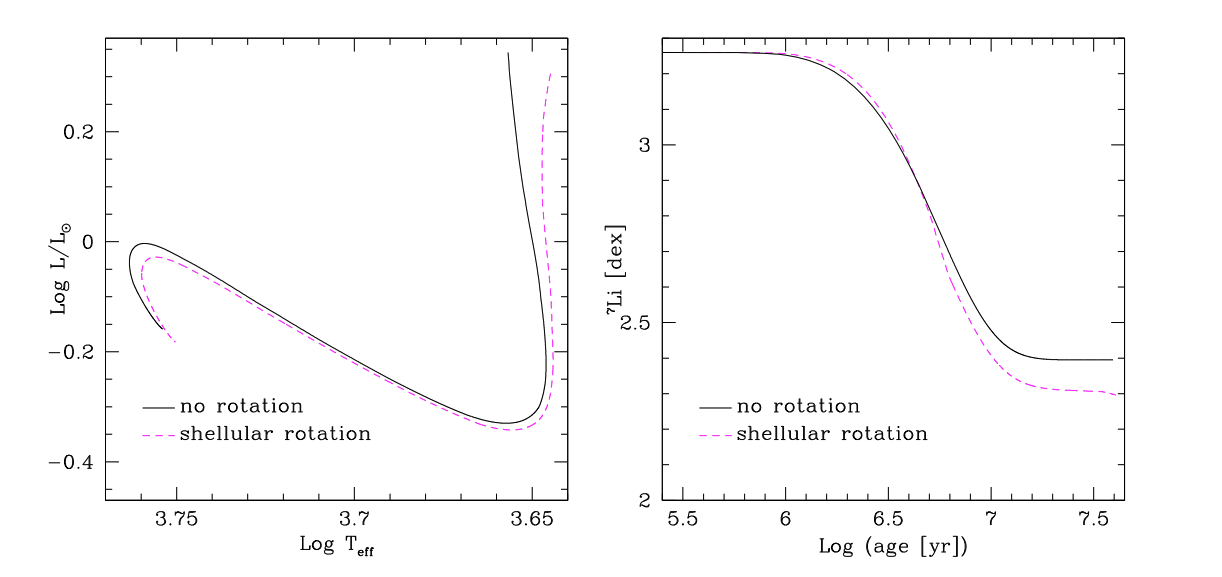
\includegraphics[width=\textwidth]{Figures/intro_figures/PMS_effect.png}
    \caption{Left: PMS HR diagram tracks of 1 M$_{\odot}$ solar metallicity models with and without rotation. The continuous line corresponds to a non-rotating model, while the dashed line corresponds to a rotating model with $\Omega = 20 \Omega_{\odot}$. The tracks end when the ZAMS is reached. Right: Surface lithium abundance with time during the PMS for the same models. Sourced from Figure 1 in \citet{eggenberger_rotation_2013}}
    \label{fig:pms_effect}
\end{figure}

Figure \ref{fig:pms_effect} (left) compares the evolutionary track of a rotating solar-type, 1M$_{\odot}$, solar metallicity, star rotating with 20 $\Omega_{\odot}$ (twenty times the mean solar surface rotation rate) against a non-rotating model of the same mass and metallicity. 
Because of the introduction of the centrifugal force, the HR path is slightly shifted towards lower effective temperatures and luminosities than a non-rotating star.

During the pre-main sequence, both the changes to the rotation impact the observed lithium abundances, which are dependent on the treatment of angular momentum transport \citep{dumont_lithium_2021}.
Figure \ref{fig:pms_effect} (right) displays the evolution of surface lithium abundance during the PMS phase for rotating and non-rotating models. 
The zero-age-main-sequence (ZAMS) surface lithium abundance of the rotating model is lower than that of the non-rotating model, indicating that including rotational effects increases lithium depletion during the PMS. 
However, during the beginning of the lithium depletion phase, the rotating model shows a slightly higher lithium content than the non-rotating one due to the centrifugal force lowering the temperature at the base of the convective envelope.

As the star develops a radiative zone at its centre, rotational mixing becomes the dominant factor in transporting lithium to deeper and hotter regions, where it is efficiently destroyed. 
This leads to a lower surface lithium abundance for the rotating model on the ZAMS compared to the non-rotating model due to the increase in differential rotation in the stellar interior during the PMS.

The duration of the disc-locking phase, which enhances differential rotation in the radiative zone, significantly impacts the sensitivity of the lithium content in rotating models. 
Longer disc lifetimes lead to lower surface lithium abundances on the ZAMS due to increased angular velocity gradients below the convective envelope, which enhance rotational mixing \citep{eggenberger_angular_2012}. 
Moreover, as the star loses more angular momentum during the longer disc-locking phase, it reaches the ZAMS with a lower surface rotational velocity, resulting in lower lithium abundance.
Therefore, a correlation between the surface velocity and lithium abundance on the ZAMS exists: stars with lower rotation rates on the ZAMS are expected to be more depleted in lithium than fast rotators on the ZAMS.

\subsubsection{Main sequence}

\begin{figure}[h]
    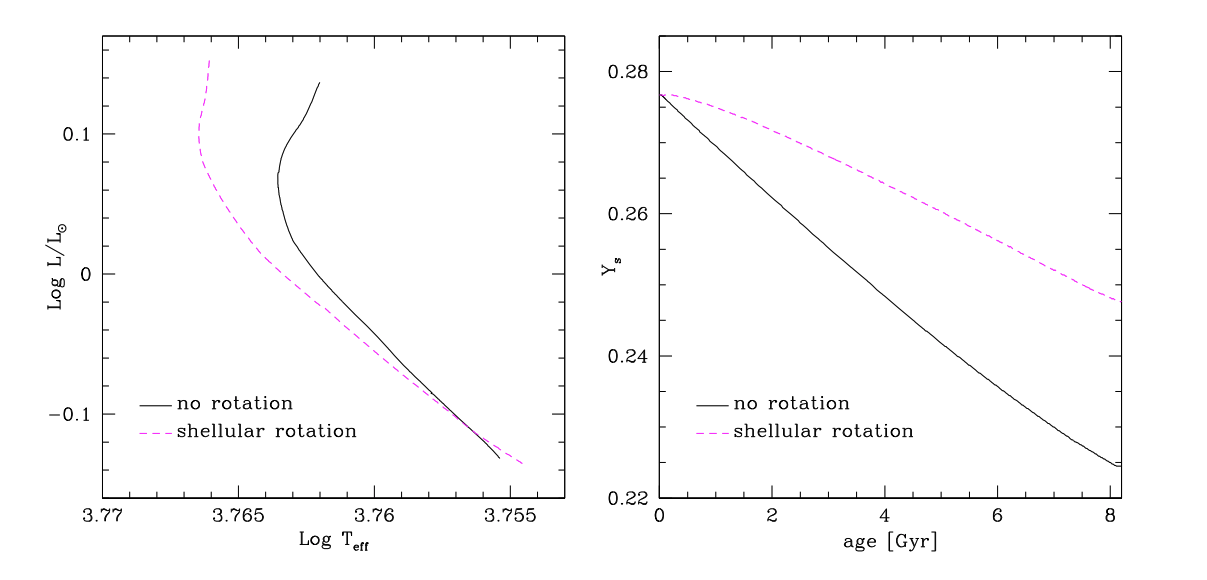
\includegraphics[width=\textwidth]{Figures/intro_figures/MS_effect.png}
    \caption{Left: MS HR diagram tracks of 1 M$_{\odot}$ solar metallicity models with and without rotation. The continuous line corresponds to a non-rotating model, while the dashed line corresponds to a rotating model with ZAMS surface velocity = 50 km/s. The tracks end when the ZAMS is reached. Right: Surface helium abundance with time during the MS for the same models. Sourced from Figure 3 in \citet{eggenberger_rotation_2013}}
    \label{fig:ms_effect}
\end{figure}

During the main sequence, rotational mixing begins to play a key role by changing the global stellar
properties. 
This is illustrated in Figure \ref{fig:ms_effect} (left), which shows the main-sequence evolution for two 1 $M_{\odot}$, solar metallicity models computed with and without rotation.
The rotating model has an initial surface velocity of 50 $km s^{-1}$

The rotating model is, like the PMS model, characterised by higher effective temperatures and slightly higher luminosities than the non-rotating model.

Figure \ref{fig:ms_effect} (right) highlights that the presence of rotational mixing counteracts the impact of atomic diffusion in the star's outer layers. 
This leads to higher helium surface abundances for the rotating model than the non-rotating model.
Consequently, the opacity in the external layers of the rotating model decreases, causing a shift towards the blue region of the HR diagram, as illustrated in Figure \ref{fig:ms_effect} (left). 
The differences in helium content between rotating and non-rotating stars become increasingly pronounced during the main sequence, resulting in significant distinctions in the HR diagram.

Furthermore, the inclusion of rotation affects the properties of the central layers of the star. As a result of rotational mixing, fresh hydrogen fuel is transported to the central core, leading to a higher central hydrogen mass fraction for rotating models than for models without rotation at a given age. This leads to an increase in the main-sequence lifetime.

\subsubsection{Post-main sequence}
Within the post-main sequence, the rotation effects are similar to the main sequence.
When rotational effects are considered, the core helium-burning phase is shifted to higher luminosity values. 
These changes are due to rotational mixing, which brings fresh hydrogen fuel into the convective core and transports helium and other H-burning products in the radiative zone.

There are no other significant enhancements in chemical abundances \citep[See Table 2. in][]{lagarde_thermohaline_2012}.
Rotation can, however, substantially affect the asteroseismic properties of low-mass red-giant stars
\citet{lagarde_thermohaline_2012, eggenberger_effects_2010}.
In particular, rotation decreases the derived stellar mass and increases the age.
Observation and identification of non-radial oscillation modes for red giants with moderate surface rotational velocities may be complicated due to non-negligible values of rotational splitting, which can be reached depending on the assumed rotation law in the convective envelope and the star's initial velocity.

\citep{eggenberger_effects_2010, lagarde_thermohaline_2012} also illustrates that the HR evolution of rotating stars can be qualitatively reproduced with enhancements to the core-overshooting parameter. 
This highlights that rotation increases the size of the convective core and changes the chemical composition of the radiative zone.


%\section{How is rotation measured?}
%\label{sec:how_rot_measured}
%
%
%Rotation can be measured in a variety of ways.
%In this Section we will outline how those measurements are made and their advantages and disadvantages.
%
%\subsection{Periodic brightness variations due to stellar spots}
%\label{sec:periodic_brightness_meas}
%
%The rotational modulation of magnetically active regions on the surfaces of active stars produce quasi-periodic variations in the disk-integrated flux.
%These brightness variations can be used to measure rotation periods for these stars.
%The measurement of rotational periods of stars using these variations is therefore a signal-processing problem by which a number of techniques have been adopted.
%
%\subsubsection{Periodogram method}
%
%
%
%
%\subsubsection{Autocorrelation Function method}
%
%\subsubsection{Gaussian Processes recovery of rotation periods}
%
%
%\subsubsection{Deep learning recovery of rotation periods}
%
%
%\subsection{Differential rotation}
%%Surface differential rotation can be inferred using a two different spectroscopic techniques. 
%%The first technique is Doppler imaging (Vogt & Penrod 1983).
%The location of individual spots has varying effects on the spectral line profile.
%Provided a star is rotating at a sufficiently high rate, the distribution of stellar spots on the surface of a star can be estimated. (Collier Cameron, Donati & Semel 2002). 
%Then, time series Doppler images provide measurements of differential rotation to be measured.
%
%The second technique is the Fourier transform method (Reiners & Schmitt 2002). In the
%FT method, the Doppler shift at different latitudes due to rotation
%can be inferred from the FT of the line profiles. Note that the star
%does not need to have starspots for this method to be used, though
%the presence of starspots might affect the results. A spectrum with
%very high S/N and high resolution is required. The method is limited to stars with projected rotational velocities in excess of about
%20 km s−1, which is the case for stars below the rotational period gap The big advantage is that latitudinal differential rotation
%can be measured from a single exposure. 

% 
% \subsubsection{ACF}

% \subsection{Spectroscopic rotational broadenings}

% \subsection{Asteroseismology}
% \label{sec:asteroseismology}

% \subsection{Duvall Law Derivation}

% Solar/stellar oscillations represent a discrete set of observations that are sensitive to its structure and rotation. This allows us to invert the structure of a star. With a solar model, differences between its mode frequencies and observation modes are weighted averages of the differences between the Sun's structure and that of the reference model; The frequency differences can then be used to infer those structural differences. Early inversions of the Sun's structure and rotation were made using inversions described by Duvall's law \citep{duvall_jr_frequencies_1988}.\\

% Duvall's law is supplemented by analyses that linearise the full set of oscillation equations describing the stellar oscillations about a theoretical reference mode.
% The $n,\ell,m$ rotational splitting is given by:
%    \begin{equation}
%     \delta_{n,\ell,m} (\Omega) = m \beta_{n,\ell} \int^R_0 K_{n,\ell}(r) \Omega(r) \,\text{d}r
%     \label{eqn:splitting}
% \end{equation}
% where, $\delta_{n,\ell,m}$ is the $n,\ell,m$ rotational splitting of the star, $K_{n,\ell}$ is the rotational kernel of the $n,\ell$ mode (determined by the stellar model), $m$ describes the spherical harmonic order, $\Omega(r)$ is the 1D rotation profile along the radial axis and $\beta_{n,\ell}$ is a normalisation constant and $R$ is the outermost radius of the star. A more thorough interpretation of the effects of rotation \citep[See][]{aerts_asteroseismology_2010} ignores the asymptotic effects and follows the perturbation in both the horizontal and radial directions. They find a general form that is dependent on the latitudinal differential rotation.
% In practice asteroseismic constraints to latitudinal differential rotation are limited to the Sun and some solar analogues \citep{bazot}. For the sake of brevity we will focus on only radial differential rotation in the derivation of rotational splittings.

   
% As a result of space-based observations from missions like \corot{} and \kepler{} , it is now possible to measure mode splittings of stars other than the Sun. However Duvall's analysis does not hold for mixed-mode oscillations and thus the generalised form is required to probe the core properties. Here we present a derivation of the asymptotic Duvall relation.

% Can derive the asymptotic expression for the rotational splitting of p-mode frequencies very simply. Following the plane wave treatment.
% Assume hydrostatic equilibrium and consider the equation of motion.
% \todo{define div}
% \begin{equation}
%     \rho \frac{\partial \vec{v}}{\partial t} + \rho \vec{v} \ \cdot \ \nabla \vec{v} = \nabla p +\rho \vec{g}
%     \label{eqn:eom}
% \end{equation}
% For now we will ignore the full equations of stellar hydrostatic equilibrium.\\
% Now consider an Eulerian perturbation about the equilibrium state
% \begin{equation}
%     p(\vec{r},t) = p_0(\vec{r}) + p' (\vec{r},t)
% \end{equation}
% It can be convenient to use the Langrangian perturbation. In the reference frame following the motion: if an element of gas is moved from $\vec{r_0}$ to $\vec{r_0}$ + $\delta\vec{r}$ the change is pressure is given as:\\
% \begin{equation}
%     \delta p (\vec{r}) = p(\vec{r_0} + \delta \vec{r}) - p_0(\vec{r_0}) + \delta r \cdot \nabla p_0 - p_0(r_0)
%      = p'(r_0) + \delta \vec{r} \cdot \nabla p_0 
% \end{equation}
% Note that the velocity is given by the time derivative of the displacement $\vec{\delta r}$,
% \begin{equation}
%     \vec{v} = \frac{\partial \vec{\delta r}}{\partial t}
% \end{equation}
% Equations for the perturbation are obtained by inserting these expressions into the full equations and neglect quantities of higher-order terms. The equation of motion becomes
% \begin{equation}
%     \rho_0 \frac{\partial^2 \delta\vec{r}}{\partial t^2} = \rho_0 \frac{\partial \vec{v}}{\partial t} = - \nabla p' + \rho_0 \vec{g}' + \rho ' \vec{g_0}
% \end{equation}
% Where, $\vec{g}' = -\nabla \Phi' (\Phi')$ satisfies the perturbed Possion's equation. And the continuity equation becomes 
% \begin{equation}
%     \frac{\partial \rho '}{\partial t} + \dive (\rho_0 \vec{v}) = 0
%     \label{eom_int}
% \end{equation}
% or by integrating with respect to time
% \begin{equation}
%     \rho' + \dive (\roh \vec{\delta r}) = 0
%     \label{eqn:ce}
% \end{equation}
% \subsubsection{Acoustic Waves}
% As the simplest equilibrium situation, consider the spatially homogeneous case. All derivatives of equilibrium quantities vanish. Here all derivatives of equilibrium quantities vanish. According to the equation of motion: gravity must be negligible. Such a situation clearly cannot be realized exactly. Consider the case where the equilibrium structure varies slowly compared with the oscillations and this becomes a reasonable approximation. Also neglect the perturbation to the gravitational potential and assume adiabatic approximation:
% \begin{equation}
%     \delta p = \frac{\Gamma_{1,0} p_0}{\rho_0} \delta \rho
% \end{equation}
% Equation \ref{eqn:eom} gives:
% \begin{equation}
%     \rho_0 \frac{\partial^2 \delta\vec{r}}{\partial t^2} = -\nabla p'
% \end{equation}
% Or by taking the divergence:
% \begin{equation}
%     \rho_0 \frac{\partial ^2}{\partial t^2} (\dive \ \vec{\delta r}) = - \nabla^2 p'
%     \label{eqn:3.43}
% \end{equation}
% div \vec{$\delta$ r} can be eliminated using the continuity equation \ref{eqn:ce}, and $p$' can be expressed in terms of $\rho$' using the adiabatic relation:
% \begin{equation}
%     \frac{\partial^2 \rho}{\partial t^2} = \frac{\Gamma_{1,0} p_0}{\rho_0} \nabla^2 \rho' = c_0^2 \nable^2 \rho'
%     \label{eqn:relation}
% \end{equation}
% Where
% \begin{equation}
%     c_0^2 = \frac{\Gamma_{1,0} p_0}{\rho_0}
% \end{equation}
% Is the sound speed. This equation has the form of the wave equation and has solutions in the form of plane waves:
% \begin{equation}
%     \rho' = a \exp [i (\vec{k} \cdot \vec{r} - \omega t)]
% \end{equation}
% By substituting this into \ref{eqn:relation} we obtain:
% \begin{equation}
%     -\omega^2 \rho' = c_0^2 \dive (i \vec{k} \rho ') = -c_0^2 \vert \vec{k} \vert ^2 \rho'
% \end{equation}
% This is a solution provided $\omega$ satisfies the dispersion relation
% \begin{equation}
%     \omega^2 = c_0^2 \vert \vec{k} \vert ^2
%     \label{eqn:nondisp}
% \end{equation}

% \subsubsection{The effect of rotation}

% We need to reconsider the derivation of the perturbation equations and include the effects of a velocity field. Assume that the equillibrium structure is stationary so all time derivatives vanish. Even with this assumption the determination of the equilibrium structure is non-trivial, owing to distortion caused by the velocity fields (e.g.
% due to centrifugal effects in a rotating star). However if we assume that the velocity $\vec{v_0}$ in the equilibrium state is sufficiently slow that terms quadratic in $\vec{v_0}$ can be neglected. The continuity equation \ref{eqn:ce} gives, because of the assumed stationarity:
% \begin{equation}
%     \dive (\rho_0 \vec{v_0}) = 0
%     \label{eqn:assum}
% \end{equation}

% Also the equation of motion (\ref{eqn:eom}) reduces to:
% \begin{equation}
%     0= -\nabla p_0 + \rho_0 \vec{g}_0
% \end{equation}
% Equation of hydrostatic support is unchanged.
% The velocity at a given point in space can be written:
% \begin{equation}
%     \vec{v} = \vec{v_0} + \vec{v}'
% \end{equation}
% Where $\vec{v}$ is the Eulerian velocity perturbation. The displacement $\vec{\delta r}$ is determined relative to the moving equillibrium fluid; related to the velocity perturbation by:
% \begin{equation}
%     \frac{\der \vec{\delta r}}{\der t} = \vec{\delta v} = \vec{v}' + (\delta r \cdot \nabla) \vec{v_0}
%     \label{eqn:8.6}
% \end{equation}
% Where $\vec{v}$ is the Lagrangian velocity perturbation and d/dt is the material time derivative. Furthermore:
% \begin{equation}
%     \frac{\der \vec{\delta r}}{\der t} = \frac{\partial \vec{\delta r}}{\partial t} + (\vec{v} \cdot \nabla) \delta r
%     \label{eqn:8.7}
% \end{equation}
% Using both of these equations the perturbed continuity equation can be written
% \begin{equation}
%     0 = \frac{\partial \rho ' }{\partial t} + \dive (\rho' \vec{v_0} + \rho_0 \vec{v'})
% \end{equation}
% \begin{equation}
%     0 = \frac{\partial}{\partial t} [\rho' + \dive (\rho_0 \delta r)] + \dive [\rho' \vec{v_0} + \rho_0 [ (\vec{v_0} \cdot \nabla)\vec{\delta r} - (\delta r \cdot \nabla)\vec{v_0}]]
% \end{equation}
% After some massaging, using \ref{eqn:assum} this can be reduced to:
% \begin{equation}
%     \frac{\partial A}{\partial t} + \dive (A \vec{v_0}) = 0
% \end{equation}
% Where
% \begin{equation}
%     A = \rho' + \dive (\rho_0 \vec{\delta r})
% \end{equation}
% This may also be written using Equation \ref{eqn:assum}
% \begin{equation}
%     \rho_0 \frac{\der}{\der t} \left(\frac{A}{\rho_0}\right) =0
% \end{equation}
% From which we can conclude that A = 0 and as such Equation \ref{eom_int} holds. This may now be written from Equation \ref{eqn:8.6}:
% \begin{equation}
%     \rho_0 \frac{\der \vec{\delta r}}{\der t} = - \nabla p' + \rho \vec{g}' + \rho' \vec{g_0}
% \end{equation}
% Or using Equation \ref{eqn:8.7}:
% \begin{equation}
%     \rho_0 \frac{\partial ^2 \vec{\delta r}}{\partial t^2} + 2 \rho_0 (\vec{v_0} \cdot \nabla) \left( \frac{\partial \vec{\delta r}}{\partial t}\right) = - \nabla p' + \rho_0 \vec{g}' + \rho' \vec{g_0}
% \end{equation}
% which replaces Equation \ref{eqn:3.43}. As the equilibrium structure is independent of time we may still separate the time dependence as an oscillatory term ($\exp (-i \omega t)$). Using solutions of this form the equations of motion become:
% \begin{equation}
%     - \omega^2 \rho_0 \vec{\delta r} - 2 i \omega \rho_0 (\vec{v_0} \cdot \nabla) \vec{\delta r} = -\nabla p' + \rho_0 \vec{g'} + \rho' \vec{g_0}
% \end{equation}
% Where the first term on the LHS corresponds to the Coriolis force and is neglected in this work. Using the acoustic wave approximations as before we obtain the dispersion relation for a plane sound wave as:
% \begin{equation}
%     \omega^2  c^2 \vert \vec{k} \vert^2 + 2 m \omega \Omega
%     \label{eqn:disp}
% \end{equation}
% This is treated as a perturbation to the Duvall relation.
% \subsubsection{The Duvall relation}
% One of the most important results of asymptotic analysis is the Duvall relation \citep{duvall_jr_frequencies_1988} from analysis of observed frequencies of solar oscillation. Starting with the dispersion relation for a plane sound wave, neglecting self-gravity, in a slowly rotating star. First consider the non-rotating case. Take Equation \ref{eqn:nondisp} as our dispersion relation and writing $\vert \vec{k}\vert^2 = k_r^2 + k_h^2$. Where $k_h$ is the length of the horizontal component of the wave vector and $k_r$ is the radial component. For a wave corresponding to a mode oscillation, $k_h$ is given by:
% \begin{equation}
%     \frac{\ell (\ell +1)}{r^2} = k_h^2
% \end{equation}
% Dropping subscripts on equilibrium quantities $k_r^2$ can be written 
% \begin{equation}
%     k_r^2 = \frac{\omega^2}{c^2} - \frac{L^2}{r^2}
% \end{equation}
% Where $L^2 = \ell (\ell + 1)$. The condition for a standing wave is roughly that:
% \begin{equation}
%     \int ^R _{r_{t}} k_r \der r = n \pi
%     \label{eqn:standing}
% \end{equation}
% Where $r_{t}$ is the inner turning point of the oscillation mode. A more careful analysis shows that $n$ should be replaced with $n+\alpha$ where $\alpha$ takes care of the behaviour near the lower turning point $r_{t}$ and at the surface. We can combine these into the Duvall relation:
% \begin{equation}
%     \int ^R _{r_{t}} \left( 1 - \frac{L^2}{\omega^2} \frac{c^2}{r^2} \right)^{1/2} \frac{\der r}{c} = \frac{(n + \alpha \pi)}{\omega}
% \end{equation}
% \subsubsection{Effect of a perturbation on acoustic-mode frequencies}
% Variations on the Duvall law from small perturbation reflect more general expressions. These perturbations can come in the form of changes to gravitational potential, changes in model/sound speed and rotation. Starting with the dispersion relation for a plane sound wave, with the addition of some \textbf{radial} perturbation $\delta_r a(r)$:
% \begin{equation}
%     \omega^2 = c^2 \vert \vec{k}\vert^2 + \delta_r a(r)
% \end{equation}
% Following the same analysis as above $k_r^2$ can be written as:
% \begin{equation}
%     k_r = \left(\frac{\omega^2}{c^2} - \frac{L^2}{r^2} - \frac{1}{c^2} \delta_r a\right)^{1/2}
% \end{equation}
% Expanding this and taking first order terms
% \begin{equation}
%     k_r \simeq \frac{\omega}{c} \left[ \left(1-\frac{L^2 c^2}{\omega^2 r^2}\right)^{1/2} - \frac{1}{2\omega^2} \left(1 - \frac{L^2 c^2}{\omega^2 r^2}\right)^{-1/2} \delta_r a \right]
% \end{equation}
% Substituting this into Equation \ref{eqn:standing}, using the $\alpha$ term to correct for boundary effects, we obtain \begin{equation}
% \frac{(n+\alpha) \pi}{\omega} \simeq \int^R _{r_t}   \left( 1 - \frac{L^2 c^2}{\omega^2 r^2}\right)^{1/2} \frac{\der r}{c} - \frac{1}{2 \omega^2} \int^R _{r_t}  \left(1 - \frac{L^2 c^2}{\omega^2 r^2}\right)^{-1/2} \delta_r a \frac{\der r}{c}
% \end{equation}
% If we neglect the term in $\delta_r a $ we retain the Duvall law. This reflects a perturbation on the Duvall law.
% We can now find the effect on the oscillation frequencies of the perturbation. Assume that the result is to change the frequency from $\omega$ to $\omega + \delta \omega$. $\alpha$ here is generally a function of $\omega$ by multiplying the perturbed Duvall law by $\omega$ and  perturbing is we obtain:
% \begin{align}
% \pi \frac{\der \alpha}{\der \omega} \delta \omega &= \delta \omega \int^R _{r_t}  \left( 1 - \frac{L^2 c^2}{\omega^2 r^2}\right)^{1/2} \frac{\der r}{c} + \omega \int^R _{r_t}  \left( 1- \frac{L^2 c^2}{\omga^2 r^2}\right)^{-1/2} \frac{L^2 c^2}{\omega^2 r^2} \frac{\delta \omega}{\omega}\frac{\der r}{c}\\
% &-\frac{1}{2 \omega} \int^R_{r_t}  \left( 1 - \frac{L^2 c^2}{\omega^2 r^2} \right)^{-1/2} \delta_r a \frac{\der r}{c}
% \label{eqn:modifiedduvall}
% \end{align}
% From this we obtain the generalised expression:
% \begin{equation}
%     S \frac{\delta \omega}{\omega} \simeq \frac{1}{2 \omega^2} \int^R _{r_t}  \left(1 - \frac{L^2 c^2}{\omega^2 r^2}\right)^{-1/2} \delta_r a \frac{\der r}{c}
% \end{equation}
% where
% \begin{equation}
%     S = \int^R _{r_t}  \left( 1 - \frac{L^2 c^2}{\omega^2 r^2}\right)^{-1/2} \frac{\der r}{c} - \pi \frac{\der \alpha}{\der \omega}
% \end{equation}

% \subsubsection{Effect of rotation on the Duvall relation}
% Assume a radial rotation profile and that is is small the modified rotation Duvall relation can be written:
% \begin{equation}
%     \pi \frac{n+\alpha}{\omega} = \int^R_{r_t} \left(1 - \frac{L^2 c^2}{\omega^2 r^2}\right)^{1/2} \frac{\der r}{c} - \frac{m}{\omega} \int^R_{r_t}  \left(1 - \frac{L^2 c^2}{\omega^2 r^2}\right)^{-1/2} \Omega(r) \frac{\der r}{c}
% \end{equation}
% Furthermore the rotational splitting can be described by the following
% \begin{equation}
%     S \delta \omega \simeq m \int^R _{r_t} \left(1 - \frac{L^2 c^2}{\omega^2 r^2}\right)^{-1/2} \Omega(r) \frac{\der r}{c}
%     \label{eqn:final}
% \end{equation}
% \subsubsection{Inverting the Duvall relation}
% Given Equation \ref{eqn:final} it is straight forward to consider $(1 - L^2c^2/r^2\omega^2)$ as a Kernel like (weighting) term. Inverting the stellar rotation profile from here requires either forward modelling or an inversion technique such as optimised local averages, regularised least square or forward modelling to obtain the rotation profile.\\
% For higher-order p modes Equation \ref{eqn:final} can be further simplified and $(1 - L^2c^2/r^2\omega^2)$ can be crudely approximated by 1. The rotational splitting relation be written:
% \begin{equation}
%     \delta_{n,\ell,m} \simeq m \frac{\int^R _{r_t}\Omega (r)\frac{\der r}{c}}{\int^R _{r_t}\frac{\der r}{c}}
% \end{equation}
% This is dependent on the model/structure of the star but is straight forward to forward model and obtain the stellar structure. The inversion is dependent on the observed modes and thus the evolutionary state of the star.


% \subsection{Average core and surface rotation rates}

%  Inverting a stellar rotation profile given measured rotational splittings is an ill-posed problem. 
%  State-of-the-art methods involve the use of linear inversion techniques. Examples of these methods include regularised least squares \citep[RLS;][]{christensen-dalsgaard_comparison_1990}, which has proven successful for the case of the Sun, and Optimally Localised Averages \citep[OLA;][]{pijpers_faster_1992,pijpers_sola_1994},
% which has also been used to accurately infer the core and surface rotation rates of stars other than the Sun. 
% Both methods rely on having a good best-fitting model to describe the sensitivity of modes to rotation at different radii. The sensitivity of rotational splittings to differing parts of a star is shown by the rotation kernels. Observational uncertainties enter any given inversion technique both from the asteroseismic rotational splittings and constraints on the stellar model. The oscillation frequencies and spectroscopic constraints underpin these uncertainties; the uncertainty in the constraints is due to the precision of the stellar model and thus the rotational kernels.\\

% OLA inversions are limited by the fact that they rely on extremely low resolution rotation profiles. Often only two measured points are available. This is a necessary condition as OLA becomes numerically unstable with increased resolution, yet is insufficient to describe the rotational gradient throughout a star.
% RLS inversions differ in that they are able to provide a mean rotational profile of a star owing to the rotational splitting. 
% However, between the well-constrained core and surface rotation rates, the mean rotational profile is limited by the regularising smoothing constant. 
% RLS can only inform the mean rotational profile according to this smoothing parameter and the inferred core and surface rotational rates are dependent on this regularisation.
%  Further constraints on the method of increased angular momentum transport post main-sequence could be implied through higher resolution inversions of the rotational profile.


% \subsection{OLA}
% \subsubsection{MOLA}
% \subsubsection{SOLA}


%todo DISCUSS WHY ONLY LOW MASS, BELOW 6500K YOU AVOID PULSATORS ETC WHICH MAKE MEASURING ROTATION PERIOD VERY HARD TO DO.
\section{Todo}
Write section on ways that observations of rotation are made - precise techniques.
\begin{itemize}
    \item To do, add some talk of differential rotation
    \item Rotation period from light curves - acf method and periodgram
    \item Doppler broadening spectroscopy
    \item Asteroseismic inference of rotation rate - OLA techniques + Forward modelling
    \item Measurement of differential rotation from doppler imaging.
\end{itemize}

Add a sentence or two about the effect of stellar spots on the observation of exoplanets

% \bibliography{references}

 % Introduction


\chapter{Constraining the Rotation Profile in a Low-Luminosity Subgiant with a Surface Rotation Measurement}
\label{chap:subgiant_ast}



\textbf{Preamble}

This chapter was originally published as:
\begin{quote}
	\citet{tanner_ast}
\end{quote}
and is presented in the form that it was published in.


\newpage


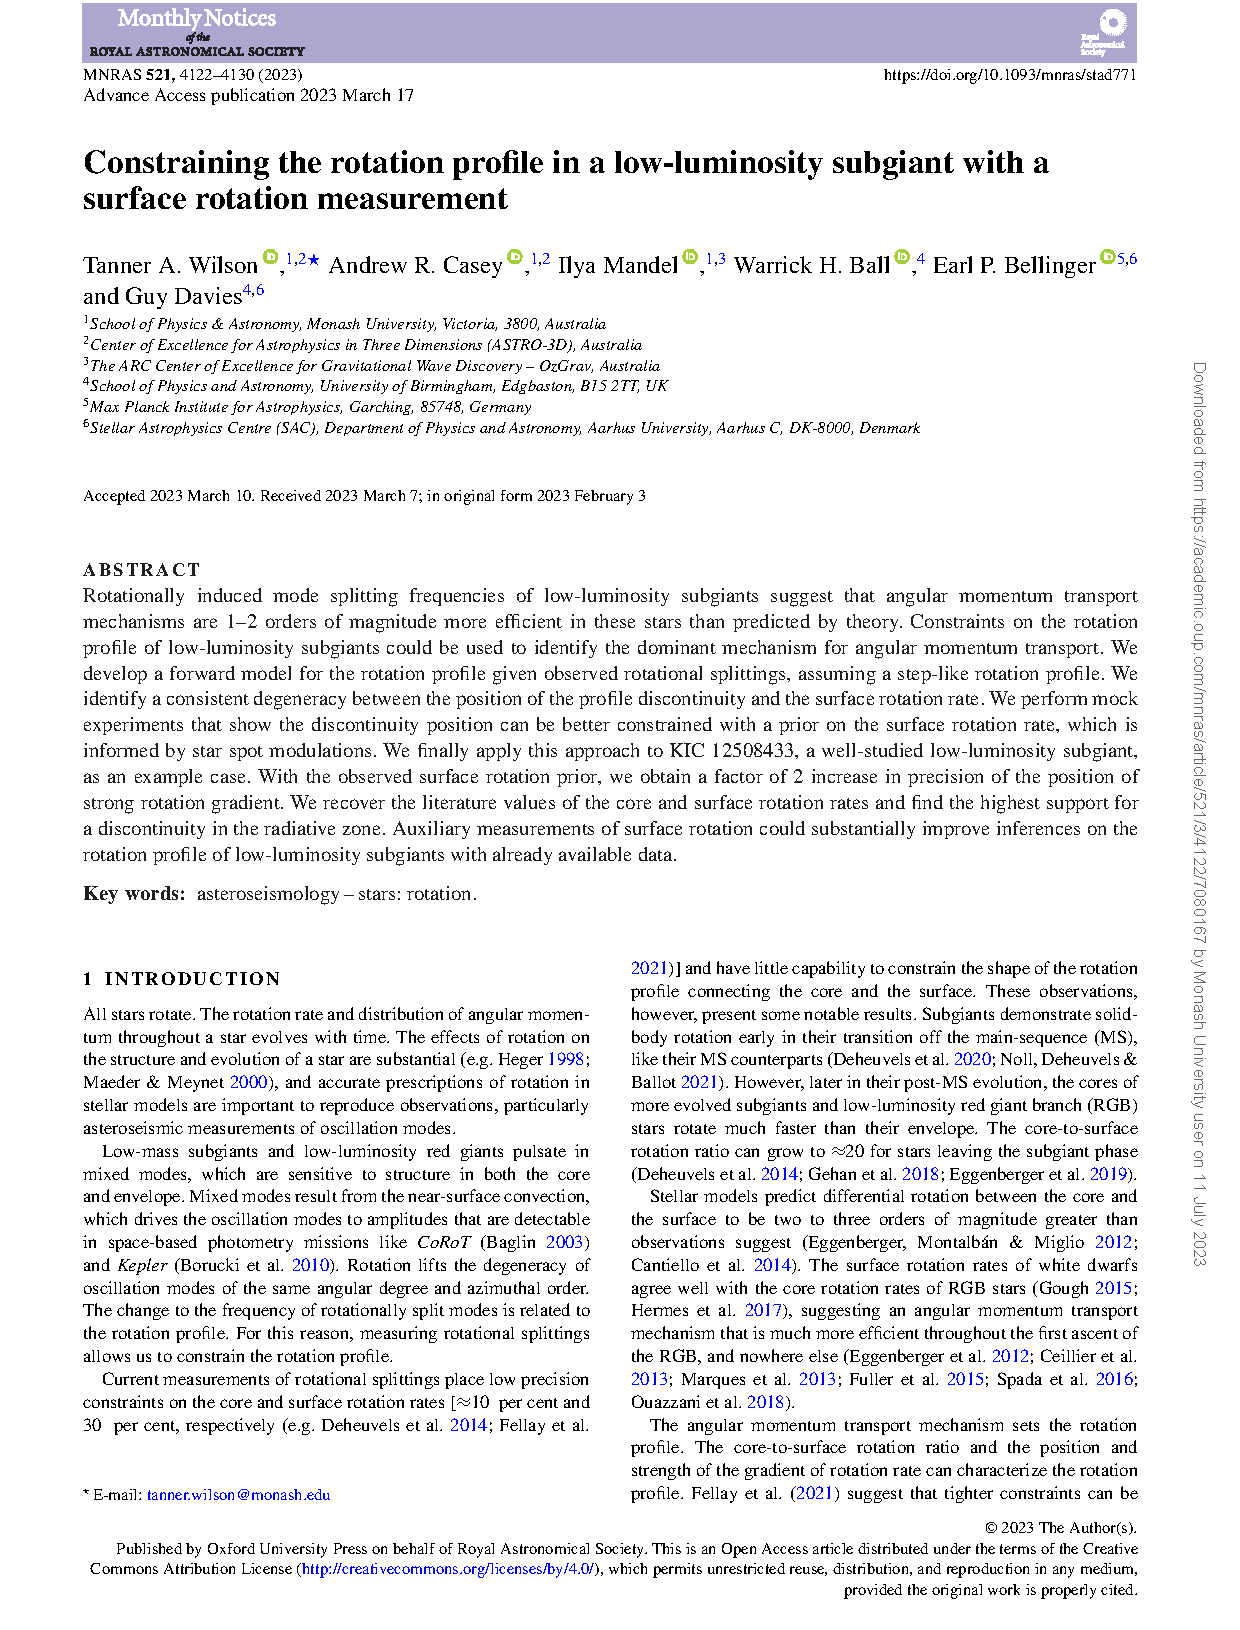
\includepdf[pages =-, pagecommand={}, scale=0.9,offset=70 -50]{Chapters/stad771-TW-subgiant.pdf}




 

\chapter{Stellar spots cause measurable variations in atmospheric metallicity}
\label{chap:stellar_spots}

\section*{Preamble}

The effects of rotation can permeate astronomy in unexpected ways.
The number of stellar spots expressed by stars is directly tied to the surface rotation rate through increased magnetic field strength.
Stars with relatively fast rotation rates express larger surface spot coverage than those with slow rotation rates \citep{cao_starspots_2022}.
While stellar spots are useful in determining the surface rotation of stars, through periodic brightness variations, they have also been obtrusive in other areas.
For example, they can mimic transits of exoplanets in light curves.

In this work, we investigate the effect of stellar spots on the inferred atmospheric parameters of stars through spectroscopy.
We adopt a simple two-temperature model of the stellar atmosphere to reflect the impact of stellar spots on the stellar atmosphere.
With this model, we generate synthetic spotted spectra of a population of stars with physically motivated stellar and spot parameters
Then, we investigate the effect of fitting spotted spectra with non-spotted models of the stellar atmosphere.
We find that, even in this simple model of the impact of spots on the stellar atmosphere stellar spots can introduce bias and scatter to inferred atmospheric parameters.
The introduced scatter is particularly impactful to the precise measurement of stellar metallicity.


This chapter was originally published as:
\begin{quote}
	\citet{tanner_ss}
\end{quote}
and is presented in the form that it was published \update{in accordance with Monash University's thesis by submission guidelines.}



\newpage


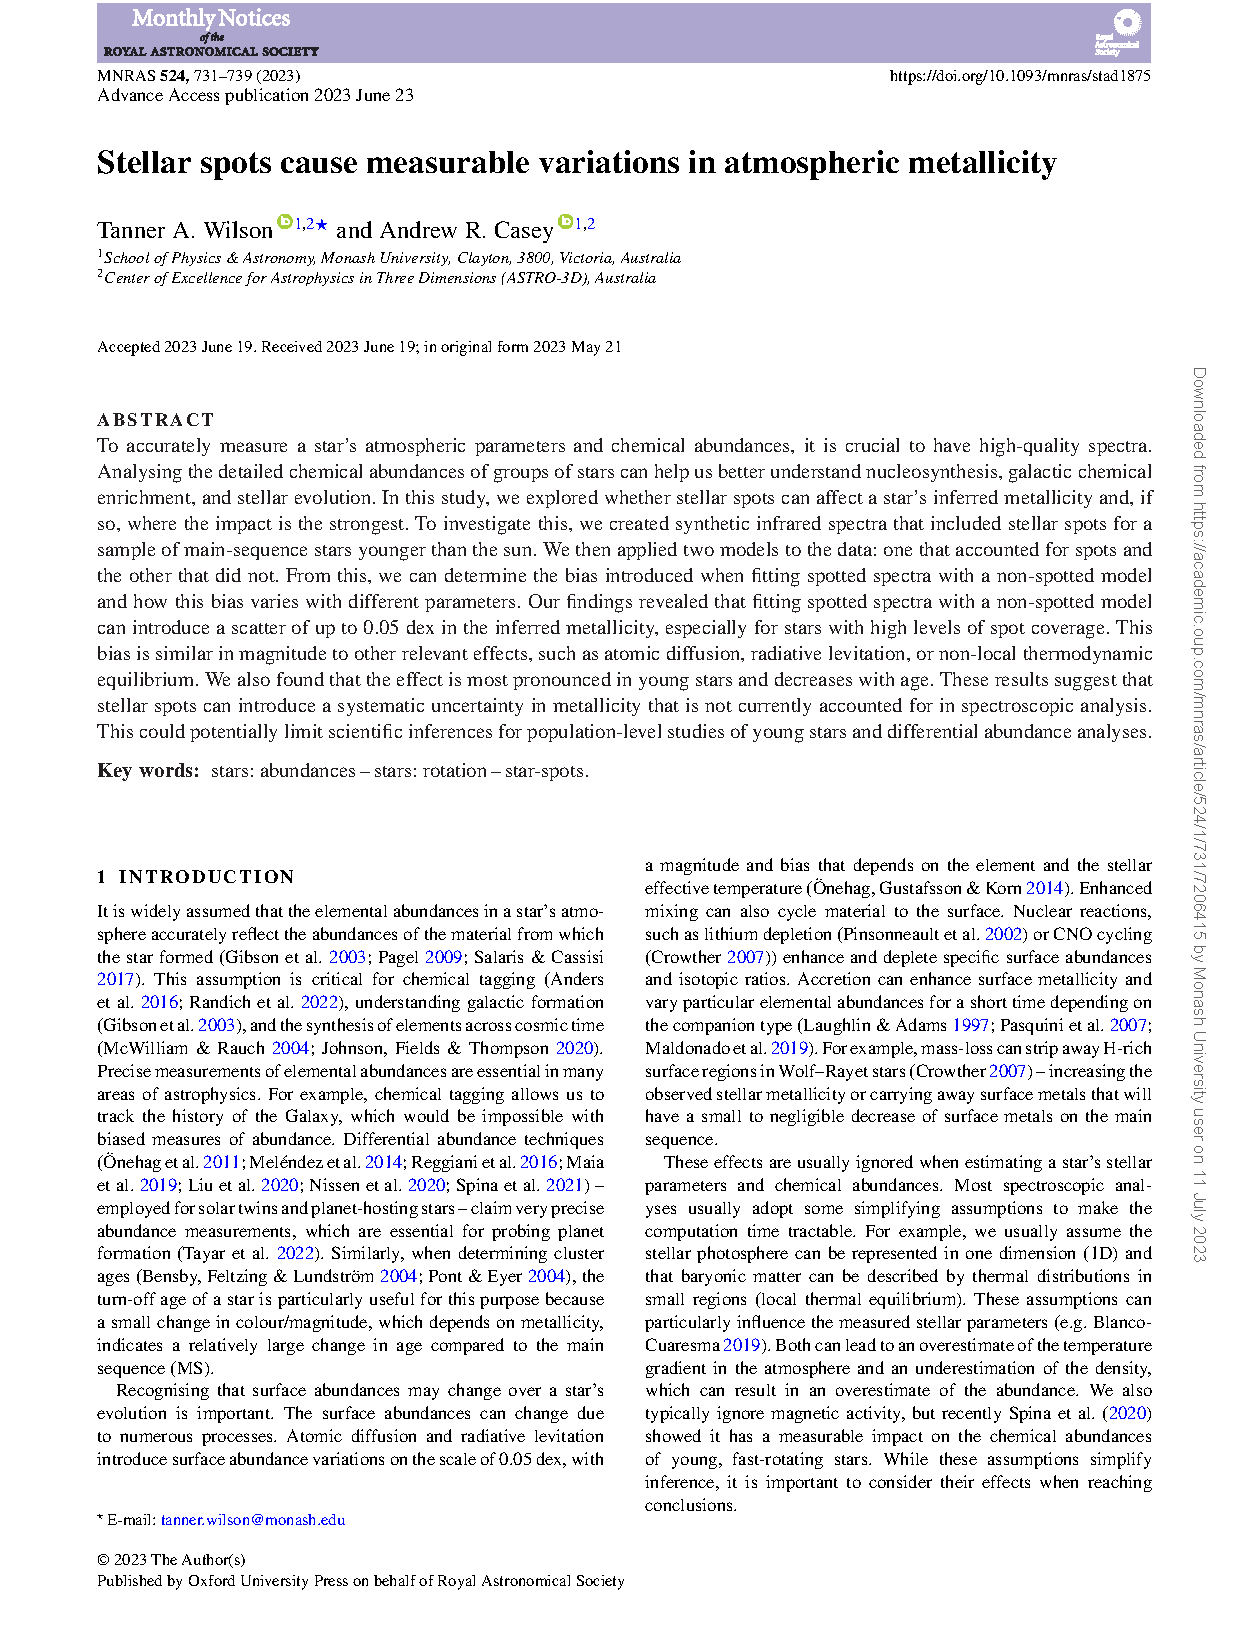
\includepdf[pages =1, pagecommand={\color{white}{\section{Introduction}}}, scale=0.9,offset=65 -50]{Chapters/stad1875-TW-SS.pdf}

\includepdf[pages =2, pagecommand={\color{white}{\section{Method}\subsection{Stellar parameters for a population of fake stars}}
\begin{figure}
    \resizebox{!}{0cm}{\begin{minipage}{\textwidth}
    \includegraphics[width=0.5\textwidth]{Figures/ss_chapter_figures/injected_hr.png}
    \caption[HR diagram of the 1500 sets of stellar parameters drawn from physically motivated distributions of mass, metallicity and age coloured by \feh.]{}
    \label{fig:HR}
        \end{minipage}}
\end{figure}
}, scale=0.9,offset=65 -50]{Chapters/stad1875-TW-SS.pdf}

\includepdf[pages =3, pagecommand={\color{white}{\subsection{Spotted spectrum generative model}}
\begin{figure*}
    \resizebox{!}{0cm}{\begin{minipage}{\textwidth}
    \includegraphics[width = \textwidth]{Figures/ss_chapter_figures/recov_tests_spot.png}
    \caption[Recovered traditional stellar parameters (\teff, \logg, \feh \ and \vsini) from fitting synthetic spotted spectra with a spotted model of the stellar atmosphere against the corresponding injected parameters.]{}
    \label{fig:recov_test}
            \end{minipage}}
\end{figure*}}, scale=0.9,offset=65 -50]{Chapters/stad1875-TW-SS.pdf}

\includepdf[pages =4, pagecommand={\color{white}{\section{Results}}
\begin{figure}
    \resizebox{!}{0cm}{\begin{minipage}{\textwidth}
    \includegraphics[width=0.5\textwidth]{Figures/ss_chapter_figures/recov_spot_param.png}
    \caption[Recovered spot parameters from the synthetic spotted spectra fitted with a spotted model of the stellar spectra against the injected parameters of the synthetic spectra.]{}
    \label{fig:recov_spot_params}
                \end{minipage}}
\end{figure}}, scale=0.9,offset=65 -50]{Chapters/stad1875-TW-SS.pdf}

\includepdf[pages =5, pagecommand={\color{white}{\section{Discussion}\subsection{Imperfect models}}
\begin{figure*}
    \resizebox{!}{0cm}{\begin{minipage}{\textwidth}
    \includegraphics[width=\textwidth]{Figures/ss_chapter_figures/recov_tests_full.png}
    \caption[The difference between the recovered traditional stellar spectra parameters (\teff, \ \logg, \ \feh \ and \vsini) from the synthetic spotted spectra fitted with both a spotted and non-spotted model of the stellar spectra against the injected parameters of the synthetic spectra]{}
    \label{fig:recov_dif}
                    \end{minipage}}
\end{figure*}}, scale=0.9,offset=65 -50]{Chapters/stad1875-TW-SS.pdf}

\includepdf[pages =6, pagecommand={\begin{figure*}
    \resizebox{!}{0cm}{\begin{minipage}{\textwidth}
    \includegraphics[width=\textwidth]{Figures/ss_chapter_figures/full_results_teff.png}
    \caption[Bias introduced to \teff\ (blue) when fitting spotted spectra with a non-spotted model against injected parameters of synthetic spectra.]{}
    \label{fig:res_teff}
    \end{minipage}}
\end{figure*}}, scale=0.9,offset=65 -50]{Chapters/stad1875-TW-SS.pdf}

\includepdf[pages =7, pagecommand={\color{white}{\subsection{When should a spotted model of the stellar atmosphere be employed?}}
\begin{figure*}
    \resizebox{!}{0cm}{\begin{minipage}{\textwidth}
    \includegraphics[width=\textwidth]{Figures/ss_chapter_figures/full_results.png}
    \caption[Bias introduced to \logg  \ (orange), \feh \ (green) and $\log$ \vsini\ (red) when fitting spotted spectra with a non-spotted model against injected parameters of synthetic spectra.]{}
    \label{fig:res_full}
        \end{minipage}}
\end{figure*}}, scale=0.9,offset=65 -50]{Chapters/stad1875-TW-SS.pdf}

\includepdf[pages =8, pagecommand={\color{white}{\section{Conclusions}}
\begin{figure}
    \resizebox{!}{0cm}{\begin{minipage}{\textwidth}
    \includegraphics[width=0.5\textwidth]{Figures/ss_chapter_figures/med_age.png}
    \caption[Bias introduced to \feh \ when fitting spotted spectra with a non-spotted model against the age of the model used to generate synthetic spectra.]{}
    \label{fig:age_mad}
            \end{minipage}}
\end{figure}}, scale=0.9,offset=65 -50]{Chapters/stad1875-TW-SS.pdf}
\includepdf[pages =9, pagecommand={}, scale=0.9,offset=65 -50]{Chapters/stad1875-TW-SS.pdf}


%
\chapter{The Intermediate Period Gap}
\label{chap:period_gap}

\section*{Abstract}


Photometric variability due to stellar spots allows astronomers to measure the surface rotation periods of stars.
Within multiple missions' rotation period samples (e.g. \kepler, \ktoo, \ZTF), there is a distinct dearth of observations of stars rotating at intermediate periods 15 $\gtrsim P_{rot} \gtrsim$ 20 days.
This dearth of observations is known as the intermediate period gap.
The position of this gap varies with the colour of the stars.
Various mechanisms have been proposed to explain the dearth of observations from stars physically \update{``jumping"} the gap through enhanced wind-braking, to stars above and below the gap representing two populations of stars, to the gap representing a minima of probability to observe rotation rate.
The exact cause of the \update{gap} is currently unknown.
In this Chapter, we propose the hypothesis that the gap represents a sudden increase in the observed rotation period of stars through the onset of equator-fast latitudinal differential rotation.
The rotation period gap can be reproduced under this mechanism with observationally derived relations between equatorial and differential rotation evolution.

\newpage

\section{Introduction}
\label{sec:intro}

Measurement of the rotation period of samples of stars allows us to understand internal mechanisms that we otherwise would not be able to probe.
%%For example, the mass-dependent core-envelope coupling and decoupling of young stars have only recently been observed by measuring the rotation period of stars with age through the rotation period distribution of clusters \citep{reinhold_rotation_2015-1}.
%An unexplained feature of the rotation period distribution of low-mass main-sequence stars comes in the form of what is known as the intermediate period gap.
The intermediate period gap represents a minimum of observations of stars with particular rotation periods measured from photometric variability due to stellar spots first observed by \citet{mcquillan_rotation_2014}.
The intermediate period gap is robust between different photometric observation missions \citep{mcquillan_rotation_2014,davenport_rotating_2017,davenport_rotating_2018,lu_bridging_2022} and multiple period detection methods applied to these missions.

The rotation period here is inferred from periodic variations to the brightness of stars from active regions coming in and out of the observer's line of sight from the rotation of its surface.
It is unknown whether the intermediate period gap occurs in other techniques to measure the rotation of stars; if it does, it would allow us to focus on particular explanations for the gap.
Rotational splittings of low-mass stars, where the gap is most apparent, have not been observed and it is currently unknown whether the intermediate period gap is also a feature observed in spectroscopic observations of surface rotation velocity.
While spectroscopic surface velocity has been measured for orders of magnitude more stars than surface rotation periods from stellar spots have, the inclination angle effect, as only \vsini\ can be measured, and uncertainties in stellar radius would smear out decreased densities of observations.
Direct observation of the intermediate period gap from spectroscopic surface velocity has not been made.

The position of the gap varies in period with respect to mass. 
The quality cuts made to data sets in which rotation period is attempted to be measured \citep[e.g. removing binaries and subgiants][]{mcquillan_rotation_2014, claytor_tess_2023} are not biased away from detecting stars within the gap.
%If the gap aligned itself with a line of constant rotation in only one mission, then the mechanism underlying the gap could be more readily explained through the selection function of said mission.
These factors suggest that the intermediate period gap represents a function of stellar evolution or an unaccounted-for problem in observing rotation periods through photometric oscillations from stellar spots.

%leading the reader.
The intermediate period gap is characterised by a number of features as shown in Figure \ref{fig:big_prawn}.
The density of stars above and below the gap is roughly constant; the density of observations drops swiftly in the gap.
The gap also aligns itself roughly with a line of constant Rossby number, suggesting a common phase evolution rather than age.
This is interesting because photometric variability drops toward the gap from below and above, suggesting a common phase of magnetic evolution.
We also observe that the dearth is most apparent for lower mass (\teff\ < 4500 K) stars.
While not shown in this plot, they are nonetheless indicative of the nature of the gap: the intermediate period gap disappears for fully convective stars \citep{lu_bridging_2022}.
Stars above and below the gap are also not significantly observationally distinct except in the rotation period.
Further, \citet{lu_bridging_2022} argued that stars above and below the gap are of similar kinematic age.
An explanation for the gap must explain all of these features.

\begin{figure}
\centering
 \includegraphics[width=\textwidth]{Figures/rot_gap_figures/big_prawn.png}
 \caption[The rotation period distribution of the \citep{mcquillan_rotation_2014} sample highlighting the features of the intermediate period gap.]{The rotation period distribution of the \citep{mcquillan_rotation_2014} sample highlighting the features of the intermediate period gap. \textbf{Top:} a 2D histogram of the logarithm of the rotation period against the effective temperature of the rotation period sample coloured by the number of stars in each bin. Here we observe the dearth of observations of rotation period for stars with \teff \ $<$ 5000 (K) between $\log_{10} \ P_{\rm{rot}\ / \ d}$ = 1 and 1.5, increasing in $P_{\rm{rot}}$ as \teff \ decreases: the intermediate period gap. \textbf{Bottom:} the logarithm of the rotation period against the effective temperature of the rotation period sample coloured by the logarithm of \rper{}. The alignment of the minimum in \rper\ and the position of the intermediate period gap is also highlighted here.  
 \textbf{Top inset:} a histogram of the logarithm of the rotation period for stars with 4000 $<$ \teff \ (K) $<$ 4200. Here, we observe the dearth of observations of stars in this effective temperature range occurs at $\sim \ \log_{10} \ P_{\rm{rot}\ / \ d} \ = 1.2$. 
 \textbf{Bottom inset:} the logarithm of the rotation period against the logarithm of \rper \ for stars with 4000 $<$ \teff \ (K) $<$ 4200. This further highlights the decrease and increase in \rper \ toward the intermediate period gap. Comparing the two inset plots, it is clear that the intermediate period gap and the decrease in \rper \ align with the same position in regards to period and effective temperature.}
 \label{fig:big_prawn}
\end{figure}


Multiple mechanisms have been proposed to explain the intermediate period gap.
\citet{mcquillan_rotation_2014} first proposed that the gap represents bimodal bursty star formation in the local \kepler{} field.
They suggest that the lower rotation period (faster rotators) prong represents a younger population, and the upper rotation period prong represents an older population, with the gap representing a minimum in star formation at a particular time.
\citet{davenport_rotating_2018} support local bursty star formation hypothesis by separating the \kepler{} rotation period distribution by distance through \gaia{} \ parallaxes.
They find that the gap appears to disappear for stars further away than 525 pc.
At those distances, observations of stars are magnitude-limited to brighter high-mass stars (M $\geq$ 0.9 M$_{\odot}$), where observations of the gap are tentative and period detection is much less precise.
If the gap extends up to these high-mass stars, then its existence can be blurred out by the imprecision of these measurements.
Their work may also support this explanation.
In the full \citep{mcquillan_rotation_2014} sample the gap disappears for high mass ($M \ \geq \ 0.8 M_{\odot}$, $B_P - R_P \ \leq \ 1.0$) stars.
In the distance limited ($\leq$ 525pc) sample, the gap appears to permeate to these higher-mass stars. 
This can be seen in the rotation period-colour distribution in the top two panels in Figure 2 of \citet{davenport_rotating_2018} where distance is limited to 525pc.

More recent works significantly disfavour the bursty star formation hypothesis.
\citet{gordon_stellar_2021} detected the gap in multiple pointings of the \ktoo \ mission. 
In contrast, \citet{curtis_when_2020} found that the open cluster Ruprecht 147 contains stars above and below the gap and a possible star detection within the intermediate period gap.
This suggests that the gap is not a coeval feature but instead a feature of the rotational evolution of low-mass stars.
\citet{curtis_when_2020} instead proposed that the gap aligns with a line of constant Rossby number ($R_o\sim 0.6$), rotation rate scaled quantity shown to be associated with the magnetic activity of stars.

As of writing, there are two leading explanations for the gap.
First, consider that the intermediate rotation period gap represents a sudden onset of extreme rotational braking.
\citet{mcquillan_rotation_2014} suggested another explanation for the intermediate period gap through a rapid spin-down - ``jumping" across the gap quickly, resulting in decreased stars' density in this period-colour space region.
For example, the rapid spin-down could be caused by core and convective envelope rotational decoupling at the upper edge of the lower prong near the rotation period gap.
In this mechanism, the core and envelope evolve independently; the rotation rate of the envelope would drop swiftly compared to a core-envelope coupled star, where angular momentum transport from the core to the surface counteracts the loss of angular momentum from magnetic braking.
Following the gap, the core and envelope then recouple, exchanging angular momentum and returning to a normal rate of magnetic braking. 
\citet{gordon_stellar_2021} argued in favour of this hypothesis based on the rotation period distribution of \ktoo{} data. 
\citet{curtis_when_2020} argued that two-zone angular momentum transport models, such as those by \citet{spada_competing_2020} can reproduce a stalled braking behaviour required to explain the lower prong of the intermediate rotation period gap. However, their model could not explain the rapid-spin down.
This hypothesis is generally supported by the tentative observation of low-mass fully convective stars permeating the gap and the observed similar ages of stars above and below the gap \citep{lu_bridging_2022}.

The other leading theory is that the gap results from a low probability of observing stars within the gap.
\citet{chahal_statistics_2022} proposes that the gap results from the low magnetic activity of stars within the gap, resulting in very few expressed stellar spots and, thus, a low probability of observing stars in the gap.
\citet{reinhold_transition_2019} and \citet{reinhold_stellar_2020}, however, proposed that the gap is caused by a transition in activity from spot dominance to bright facula dominance \footnote{This work differentiates between the rotation brightness modulation and brightness modulation from the stellar activity cycle. Stellar activity modulation refers to the long-term evolution of average brightness due to stellar spots and faculae rather than variations on the rotational time scale.}.
They suggest that as a star spins down and the magnetic field topology changes, the initially strong and long-lived spots are replaced by smaller, short-lived spots surrounded by bright faculae.
In such a scenario, the photometric variability amplitude decreases because of the partial cancellation by the increase and decrease in brightness from the faculae and spots.
Hence, the stars with small photometric variability will not be detected.
These mechanisms are supported by the gap aligning with a line of constant Rossby number and by the photometric variability reaching a local minimum surrounding the gap.


%On the other hand, if the gap results from a low probability of observing stars within the gap, we have undoubtedly observed gap stars, spectroscopically or asteroseismically, that we do not know are gap stars.
%Therefore, whether gap stars are peculiar - photometrically, spectroscopically or asteroseismically - is unknown.
%Gap stars may have been previously flagged as peculiar, but the link between the gap and these stars has never been made.
%On the other hand, gap stars may not be otherwise peculiar - chemically or, say, in terms of magnetic activity.
%If indeed they are not otherwise peculiar, then, oxymoronically, the reason for their lack of observation raises more questions about the mechanism underlying the gap.

%\update{If either of these theories are correct they have implications for the evolution of rotation and magnetic activity within stars.
%There is, however, little evidence to confirm either of their involvement in the observation of the intermediate period gap.}
%We propose a previously uninvoked mechanism: the onset of latitudinal differential rotation.
%
%Stars, most concretely for the Sun, have been observed to express latitudinal differential rotation.
%Further, stars express latitudinally distributed spots across their surface.
%Which raises the question: what is the ``surface rotation period'' of a star?
%Radially symmetric (1D) models of rotating stellar evolution provide a measure of the ``average" surface rotation rate of stars, but then if the rotation profile varies latitudinally, what does that surface rotation rate map to?
%The observed rotation rate of stars measured from stellar spots is generally taken as the average rotation rate where stellar spots are expressed \citep{santos_surface_2021}, but how well do those values map to models of stellar rotation?
%The terms are ill-defined, but we intend to bridge the gap between these two facets by considering the effect that latitudinal differential rotation has on the observed rotation periods of stars.
%Specifically, whether a swift transition from flat to latitudinally differentially rotating introduces significant variations to the observed rotation period, resulting in the intermediate period gap.

If either of these theories proves correct, they have significant implications for our understanding of the evolutionary processes governing stellar rotation and magnetic activity. 
However, it is important to note that there is currently limited empirical evidence to support the involvement of either theory in explaining the phenomena observed in the intermediate period gap of stars.
We propose a previously unexplored mechanism to explain the intermediate period gap: the initiation of latitudinal differential rotation within stars. 

Notably, observational data, particularly for the Sun, has indicated the existence of latitudinal differential rotation in stars. Additionally, stars exhibit the presence of spots distributed across their surfaces, raising an intriguing question: How should we define the ``surface rotation period" of a star?
Traditional radially symmetric (1D) models of stellar evolution offer a means to calculate an ``average" surface rotation rate for stars. However, if the rotation profile varies across latitudes, the relation between the average rotation rate and the latitudinal rotation profile becomes less clear.
Currently, the observed rotation rate of stars, as determined from the presence of stellar spots, generally represents the average rotation rate where these spots are visible \citep{santos_surface_2021}.
\citet{aigrain_hare_2015} qualified this idea.
They performed a hare-and-hounds exercise with simulated light curves of rotating stars with latitudinal differential rotation and variable latitudinal distribution of stellar spots.
Their simulations include a prescription for the latitudinal range of the spot distribution, as well as lifetime and the effect on the brightness of each stellar spot.
While a range of rotation periods can be measured owing to latitudinal differential rotation and latitudinal distribution of stellar spots, they find that the ``measured" rotation period tends to be dominated by the largest spots.
For direct comparison between the injected range of rotation periods and measured rotation periods, each spot was assigned a weight proportional to its effective area.
The ``average" period was then defined as the median weighted period from the latitude of each spot.
They found, in general, that the average and measured rotation periods generally agree.
Suggesting that, indeed, the measured rotation periods of stars vary with latitudinal differential rotation and that if the scale of latitudinal differential rotation grows swiftly, then the measured rotation period will also grow swiftly.
It is also worth noting that they found that the measurement of the scale of differential rotation is untenable with current data and methods.

\update{Qualitatively, observations \citep[see, e.g.,][]{saar_starspots_2011, benomar_nearly_2015, benomar_asteroseismic_2018, bazot_latitudinal_2019, hall_weakened_2021} and magnetohydrodynamic models of stars including latitudinal differential rotation \citep[see, e.g.,][]{brun_powering_2022} suggest three regimes of latitudinal differential rotation dependent on Rossby number.
Their results suggest fast-rotating stars ($R_o < 0.45$) support quenched, latitudinally flat\footnote{Or rather, close to latitudinally flat.} rotation profiles.
In this regime, the scale of equator-fast differential rotation, defined as the absolute difference between the rotation rate at the equator and at a latitude of 60$^{\circ}$ divided by the equator rotation rate, increases with $R_o$.
The scale of differential rotation swiftly grows in this regime until it saturates, resulting in intermediate rotating stars ($0.45 \ \leq \ R_o \ \leq \ 2$) expressing constant scale equator-fast differential rotation.
As a star approaches $R_o \sim 2$, meridional transport of angular momentum from the equator to the pole is expected to slow the rotation rate near the equator \citep{amard_rotating_2016}.
This, in combination with angular momentum loss through magnetised stellar winds, is expected to result in a supposed transition from equator-fast to equator-slow latitudinal differential rotation\footnote{While this transition is theoretically expected, however, equator slow differential rotation has not been observationally verified.}.
The relationship between the scale of differential rotation in this regime is unknown due to a lack of observations of equator-slow differential rotation.}

Interestingly, the transition from latitudinally flat rotation profiles to equator-fast rotation profiles occurs near $R_o \sim 0.5$, the Rossby number where the rotation period gap occurs.
If latitudinal differential rotation becomes significant at this point in the evolution of rotation of a star, then the rotation period gap may reflect a sudden increase in average, and thus observed, surface rotation period from that onset.
In this work, we qualitatively investigate this as a possible mechanism underlying the intermediate period gap by creating a physically motivated observed rotation period distribution under the differential rotation relationships proposed by \citet{saar_starspots_2011} and \citet{brun_powering_2022}.
In Section \ref{sec:methods}, we describe the adopted relationships between latitudinal differential rotation and Rossby number, our choices of stellar parameters, as well as our adopted method to calculate an observed rotation period.
In Section \ref{sec:results}, we present the observed rotation period distributions of the synthetic sample, compared to the observed \kepler \ rotation period distribution.
Finally, in Sections \ref{sec:discussion} and \ref{sec:conclusione}, we place those results into context by discussing the implications of our discovery, discuss the impact of the uncertain model parameters, and propose extensions to this work.


\section{Methods}
\label{sec:methods}

\subsection{Generative model}

The scale and sign of differential rotation varies with $R_o$.
To calculate $R_o$ we require the first evaluate the convective turnover timescale ($\tau_c^{\rm{CS}}$) of our sample using the scaling relation derived in \citet{cranmer_testing_2011},
\begin{equation}
	\tau_c^{\rm{CS}} = 314.24 \ \exp\left[ -\frac{T_{\rm{eff}}}{1952.5\rm{K}} - \left( \frac{T_{\rm{eff}}}{6250 \rm{K}}\right)^{18}\right] + 0.002 d
\end{equation}
from this we calculate $R_o$ ($R_o = P_{\rm{surf}}/\tau_c^{\rm{CS}}$).

We adopt the three different piecewise functions to represent the evolution of the scale of differential rotation between the equator and at a latitude of 60$^{\circ}$.
The first is the observational trend described in \citet{saar_starspots_2011}, where the scale of differential rotation grows with $R_o^{2.5}$ while $R_o \ \leq \ 0.45$ and is constant above this limit,
\begin{equation}
\label{eq:rot_saar}
{\centering
\frac{\Delta\Omega}{\Omega_{\rm{eq}}} = \left\{
\begin{array}{ll}
  0.2/(0.45^{2.5}) \ R_o^{2.5}& R_o\leq 0.45 \\
  0.2 & 0.45 \leq R_o < \ 1.3\\
  -0.2 R_o^q \ / \ 1.6^q + 0.4 & 1.6 \leq R_o < \ 2.3\\
  -0.2 & R_o > 2.3
\end{array} 
\right.}
\end{equation}
where $\Delta \Omega$ is the difference between the equator rotation rate and the rotation rate at a latitude of 60$^{\circ}$ and $\Omega_{\rm{eq}}$ is the equator surface rotation rate ($2\pi/P_{\rm{eq}}$).
We have ensured continuity between latitudinally-flat ($R_o \ \leq \ 0.45$), equator-fast rotation (0.45 $<$ $R_o \ \leq 1.6$) with the prefactor $0.2 \ / 0.45^{2.5}$ as well as in the transition from equator-fast to equator-slow rotation ($R_o \ \sim \ 2$) through the introduction of the term $-0.2 \ R_o^q \ / \ 1.6^q + 0.4 R_o$ when $1.6 \leq R_o < 2.3$.
The term $-0.2 \ R_o^q \ / \ 1.6^q$ slowly decreases $\frac{\rm{d}\Omega}{\Omega_{\rm{eq}}}$ above $R_o \ = \ 1.6$, while the factor of $0.4$ ensures a continuous transition when the scale of differential rotation transitions to saturated equator slow rotation at $R_o \ = \ 2.3$.
Here, $q$ is the solution to $0.2 \left(2.3/1.6\right)^q + 0.4 \ = \ -0.2 $ ($q \sim 3$).
This results in a transition from equator-fast to equator-slow rotation at $R_o \sim 2$.

The transition between equator-fast and equator-slow rotation requires some discussion.
There are no statistically significant observations of equator-slow latitudinal differential rotation.
Models predict a transition from equator-fast to equator slow-differential rotation around the solar Rossby number, $R_o \sim 2$, \citep{brun_powering_2022}; however, due to the limited number of these models and their high-computational requirements, the exact nature of this transition is unknown.
Our prescription for this transition is, therefore, not physically motivated.
That being said, we have attempted to avoid what we believe to be an unphysical instantaneous transition by including the power law transition explained above.
As this work constitutes a qualitative exploration of the qualitative effect of differential rotation on the observed rotation rate of stars, we will only comment on the general effects of this transition on the observed distribution of rotation periods under the effect of latitudinal differential rotation.

The other two relations we adopt reflect two cases for the transition of the scale of differential rotation that are steeper than the \citet{saar_starspots_2011} relation that fall within the range suggested by the edges of the scale of differential rotation in \citet{brun_powering_2022} (See Figure 8 in their work).
These relations are:
\begin{equation}
\label{eq:rot_pow4}
{\centering
\frac{\Delta\Omega}{\Omega_{\rm{eq}}} = \left\{
\begin{array}{ll}
  0.35 \ / \ (0.45^4) R_o^4& R_o\leq 0.45 \\
  0.35 & 0.45\leq R_o\leq 1.6 \\
  -0.35 \ R_o^q  \ / \ 1.6^q + 0.7 & 1.6 \leq R_o < \ 2.3\\
  -0.35/(2^2) R_o^2& 2.3\leq R_o \\
\end{array} 
\right.}
\end{equation}

and

\begin{equation}
\label{eq:rot_pow6}
{\centering
\frac{\Delta\Omega}{\Omega_{\rm{eq}}} = \left\{
\begin{array}{ll}
  0.35 \ / \ (0.45^8) R_o^8& R_o\leq 0.45 \\
  0.35 & 0.45\leq R_o\leq 1.6 \\
  -0.35 R_o^q \ / \ 1.6^q + 0.7 & 1.6 \leq R_o < \ 2.3\\
  -0.35/(2^2) R_o^2 & 2.3\leq R_o \\
\end{array} 
\right.}
\end{equation}
we have ensured continuity between latitudinally flat and equator-fast rotation regimes with the prefactors $0.35 \ / \ (0.45^8)$ and $0.35 \ / \ (0.45^4)$ and we have adopted again adopted continuous variation between the equator-fast and equator-slow regimes using the term $-0.35 \ R_o^q \ / \ 1.6^q + 0.7$ for $1.6 \ < \ R_o \ < \ 2.3$.
Here, $q$ retains the same value as in Equation \ref{eq:rot_saar}.
We have chosen these two relations to investigate the effect of the steepness of the relation between differential rotation and $R_o$ on the observed rotation period distribution and the effect of an increase to the scale of equator-slow differential rotation for $R_o > 2$.
These two relations are consistent with the range of the scales of differential rotation suggested by the magnetohydrodynamic models of \citet{brun_powering_2022}.

The relations we adopt in this work are shown in Figure \ref{fig:compar_diffrot}, where we show the relation determined in \citet{saar_starspots_2011} (Equation \ref{eq:rot_saar}) in orange, and the two steeper relations (Equations \ref{eq:rot_pow4} and \ref{eq:rot_pow6}) in green and purple respectively.

\begin{figure}
\centering
 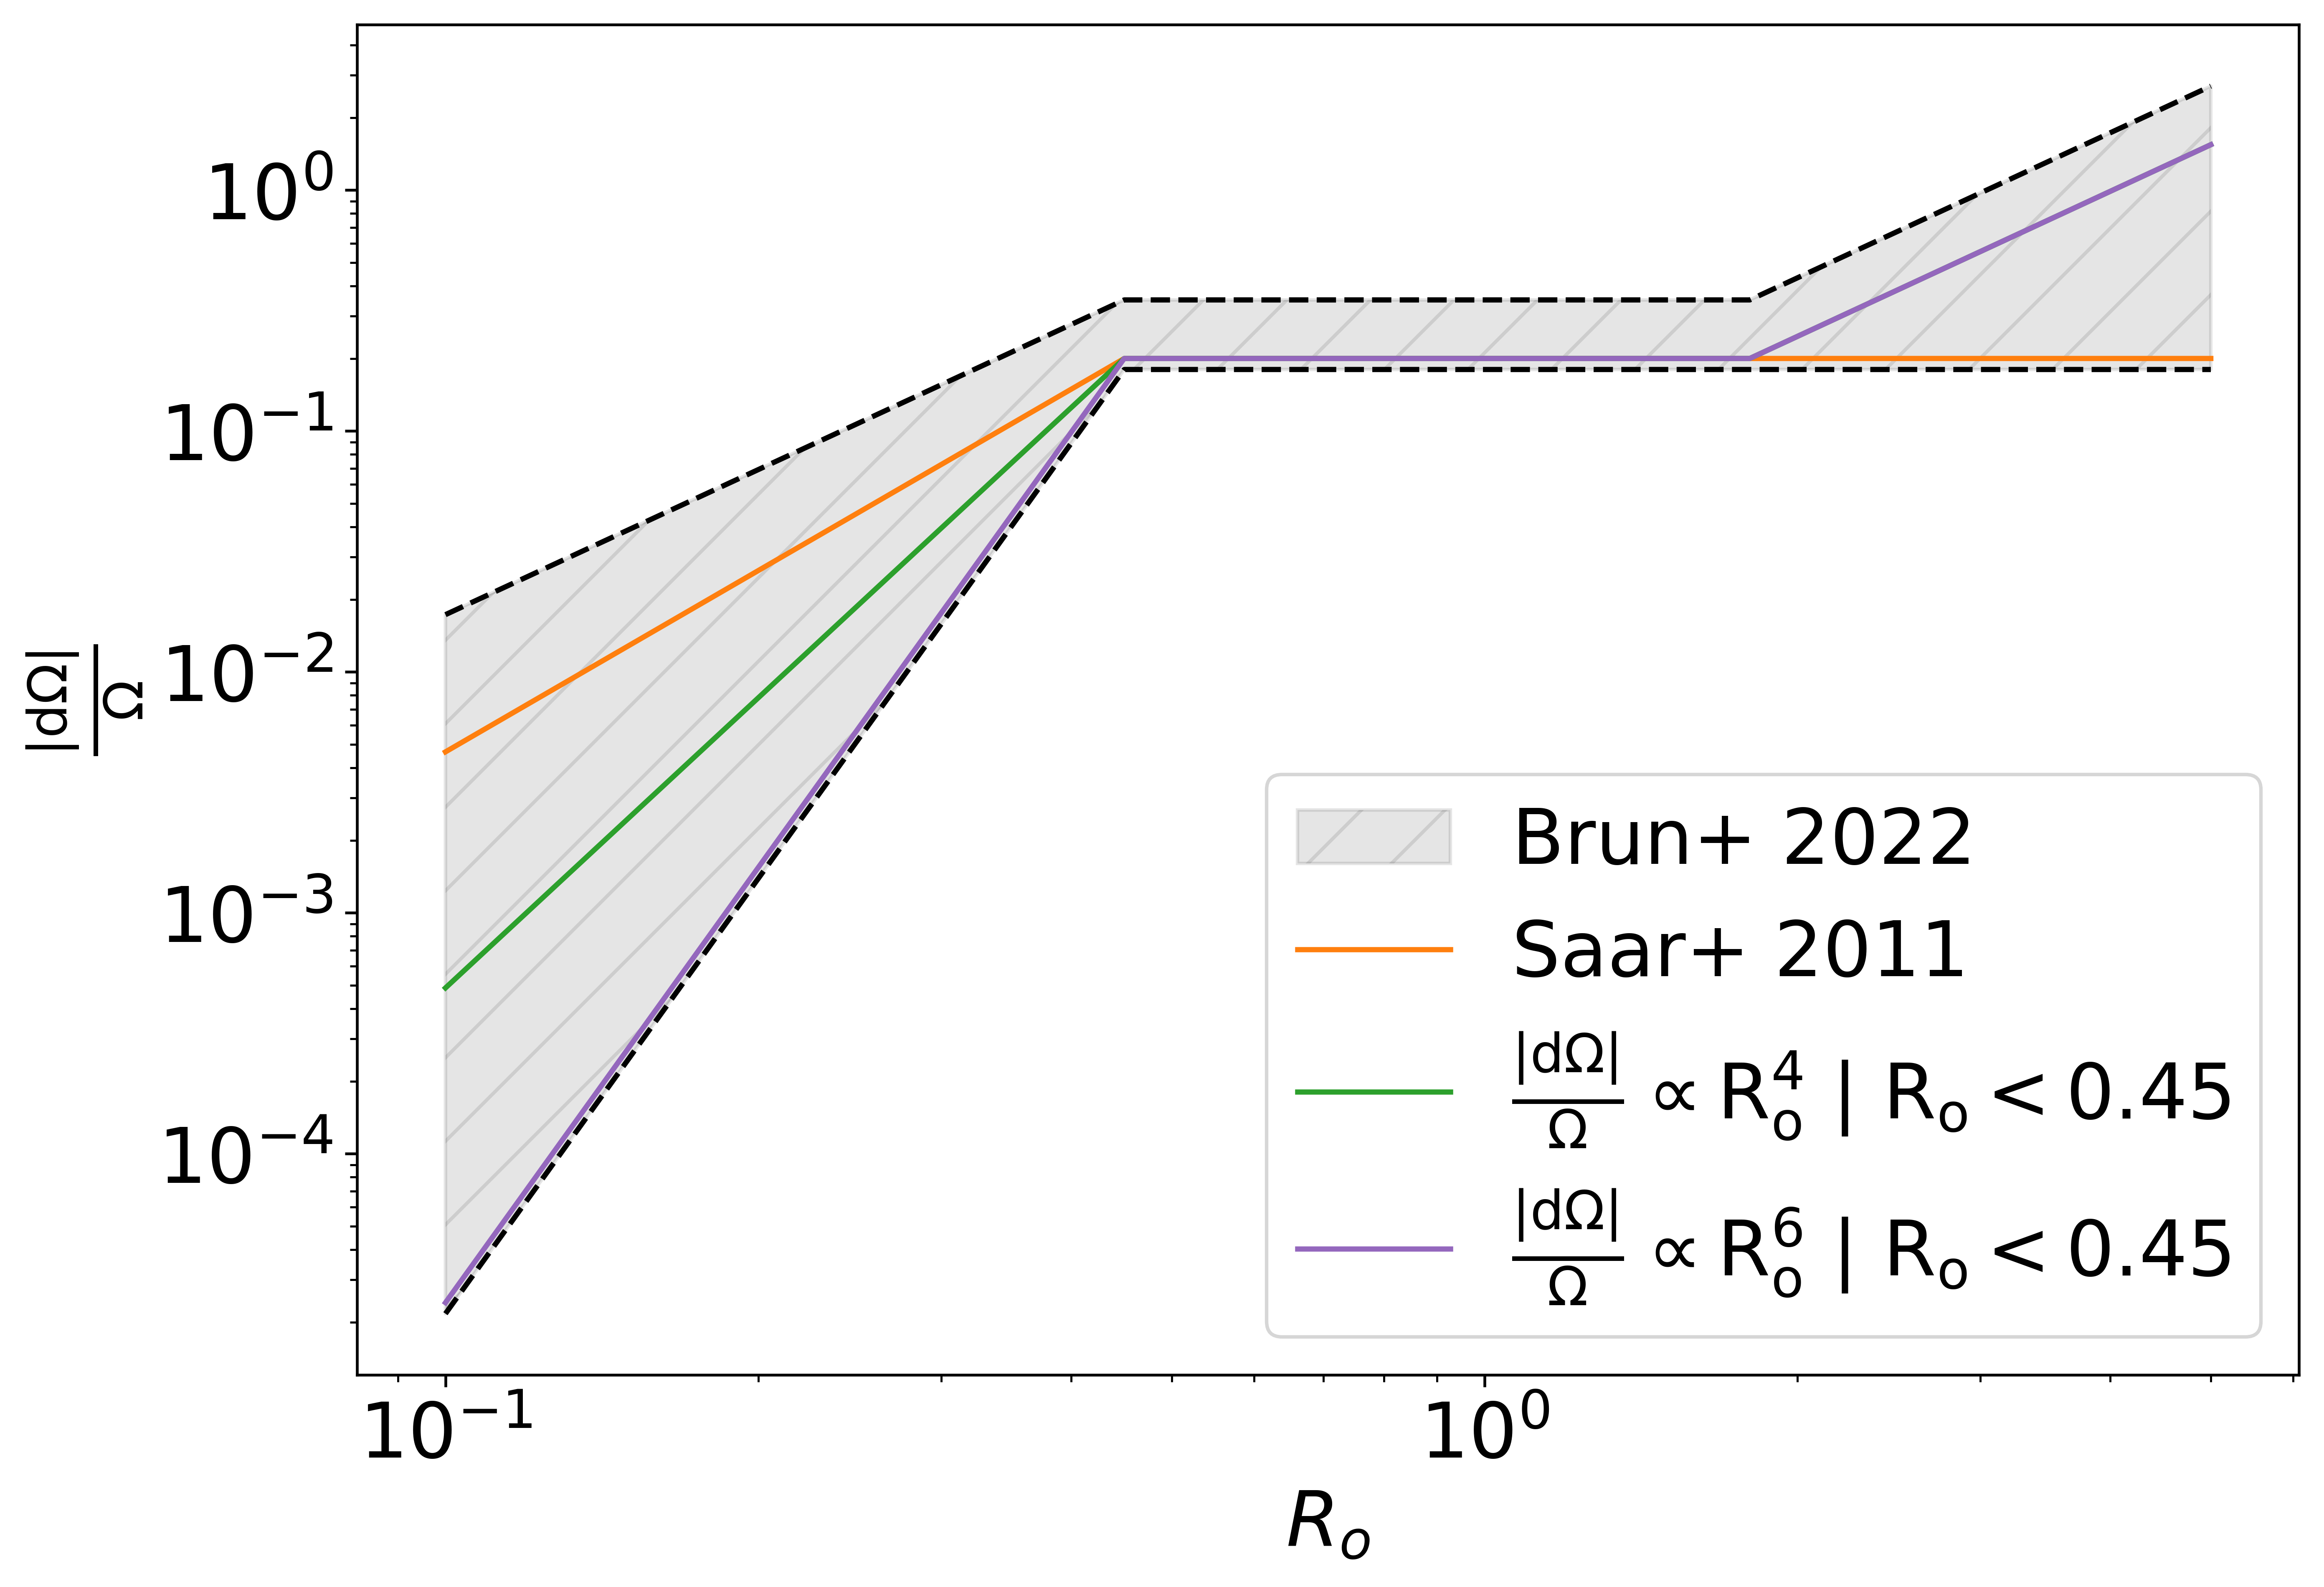
\includegraphics[width=\textwidth]{Figures/rot_gap_figures/comparison_diffrot.png}
 \caption[The various relationships between latitudinal differential rotation and the stellar $R_o$ adopted in this work.]{
 	The various relationships between latitudinal differential rotation and the stellar $R_o$ adopted in this work. We compare the observationally derived relation from \citet{saar_starspots_2011} (Equation \ref{eq:rot_saar}, orange) and two steeper relations (Equations \ref{eq:rot_pow4} and \ref{eq:rot_pow6}, green and purple, respectively). The scale of differential rotation is greater for the latter two relations, and we have an increase to the scale of differential rotation for $R_o\geq2$. All three relations are consistent with the magnetohydrodynamic investigations into stellar differential rotation from \citet{brun_powering_2022}.
}
 \label{fig:compar_diffrot}
\end{figure}

We adopt a second-order equator-fast differential rotation profile with the rotation rate with latitude, $\theta$,
\begin{equation}
  \label{eq:obs_eq}
  \Omega\left(\theta\right) = \Omega_{\rm{eq}} - \frac{\Delta \Omega}{\sin^2 60^{\circ}} \sin^2{\theta}
\end{equation}
where the factor $\frac{1}{\cos^2{60^{\circ}}}$ ensures that the rotation rate is $\Delta \Omega + \Omega_{\rm{eq}}$ at $\theta \ = \ 60^{\circ}$ (from the definition of $\Delta \Omega$).
Given the equatorial rotation rate, this provides us with our expression for the latitudinal differential rotation profile of our stars.

We calculate the ``observed" rotation rate from the integral of the rotation rate given a distribution of stellar spots on a star's surface divided by the star's surface area, both calculated where the stellar spots are expressed.
Indeed, this value does not directly map to what would be measured by analysing the light curve. 
This is because, as suggested in \citet{aigrain_hare_2015}, the measured rotation period of stars can be dominated by stochastic, long-lived large stellar spots.
Two stars with the same underlying spot probability distribution can have widely different measured periods, depending on when they are observed.
Our calculation of the observed period here is, therefore, a qualitative representation of the effect of latitudinal differential rotation on the observed period.

An accurate prescription for variations in the latitudinal distribution of the stellar spots is also unknown.
The latitudinal distribution of stellar spots on the surface of the Sun is well known \citep[see, e.g.,][]{maunder_note_1904,hathaway_solar_2015}.
While we could adopt a solar distribution, this does not account for variations between stars.
For example, the latitudinal distribution of active regions varies along the stellar magnetic cycle \citep[see, e.g.,][ and references therein]{grijs_stellar_2021}.
Further, adopting such a distribution would not account for star-to-star variations with stellar mass, equator rotation rate, and the scale of differential rotation both radially and latitudinally.
For this reason, the treatment of the distribution of stellar spots is a major source of uncertainty in our work.
For now, we adopt a uniform distribution of stellar spots between the latitudes of $0^{\circ}$ and $60^{\circ}$.

We will also assume here that all stars in our sample are viewed equator-on.
While this is not the case for all stars, the rotation period gap is not an effect of the observation angle.
Line-of-sight differences due to stellar inclinations can also introduce biases to the observed rotation periods.
Stars must be viewed close to equator-on for stellar spots to introduce significant variations to the light curve as a star rotates.
Further, inclination angles are uniformly distributed in $\cos{i}$, and  
Therefore, most stars with observed rotation periods are close to equator-on.

The average rotation rate is calculated from the integral of the rotation rate divided by the surface area both over the maximum and minimum latitudes that the spots are expressed,
\begin{equation}
\label{eq:inte}
	\Omega_{\rm{obs}} = \int^{\theta_{\rm{max}}}_{\theta_{\rm{min}}} \Omega(\theta) \cos(\theta)^2 \rm{d}\theta \ / \ \int^{\theta_{\rm{max}}}_{\theta_{\rm{min}}} \cos(\theta)^2 \rm{d}\theta
\end{equation}
where rotation rate is independent of radius and azimuthal angle, and their contributions cancel.
Here $\theta_{\rm{max}}$ and $\theta_{\rm{min}}$ are the upper and lower bounds of the distribution of spots on the surface of the star.
The factor $\cos(\theta)^2$ arises by accounting the angle between the surface normal and line-of-sight ($\cos(\theta)$) and the spherical coordinate Jacobian ($\cos(\theta)$)
As the rotation profile is symmetric about the equator of rotation, we only need to calculate the contribution to the rotation rate in one hemisphere.

We begin by comparing the effect of each of the chosen relations between differential rotation and $R_o$ on the observed rotation period of a $0.7 M_{\odot}$ star in Figure \ref{fig:comp_per}.
Latitudinal differential rotation introduces significant biases to the observed rotation periods.
The number of stars with similar observed rotation periods is related to the gradient of $P_{\rm{obs}}$ against $P_{\rm{eq}}$: larger gradients result in an under-density of observations while smaller gradients result in an over-density of observations both relative to the injected equatorial period distribution.
The growth of differential rotation below $R_o < 0.45$ occurs where $P_{\rm{eq}} < 15$ d.
Steeper relations of $R_o$ with the scale of differential rotation in this domain result in a quicker growth in observed rotation periods for the same equatorial rotation period.
The steeper the growth of the observed rotation period, the lower the number of stars that would be observed with that rotation period.
The transition from equator-fast to equator-slow differential rotation is shown at $P_{\rm{eq}} \ \sim \ 80$ d.

\begin{figure}
\centering
 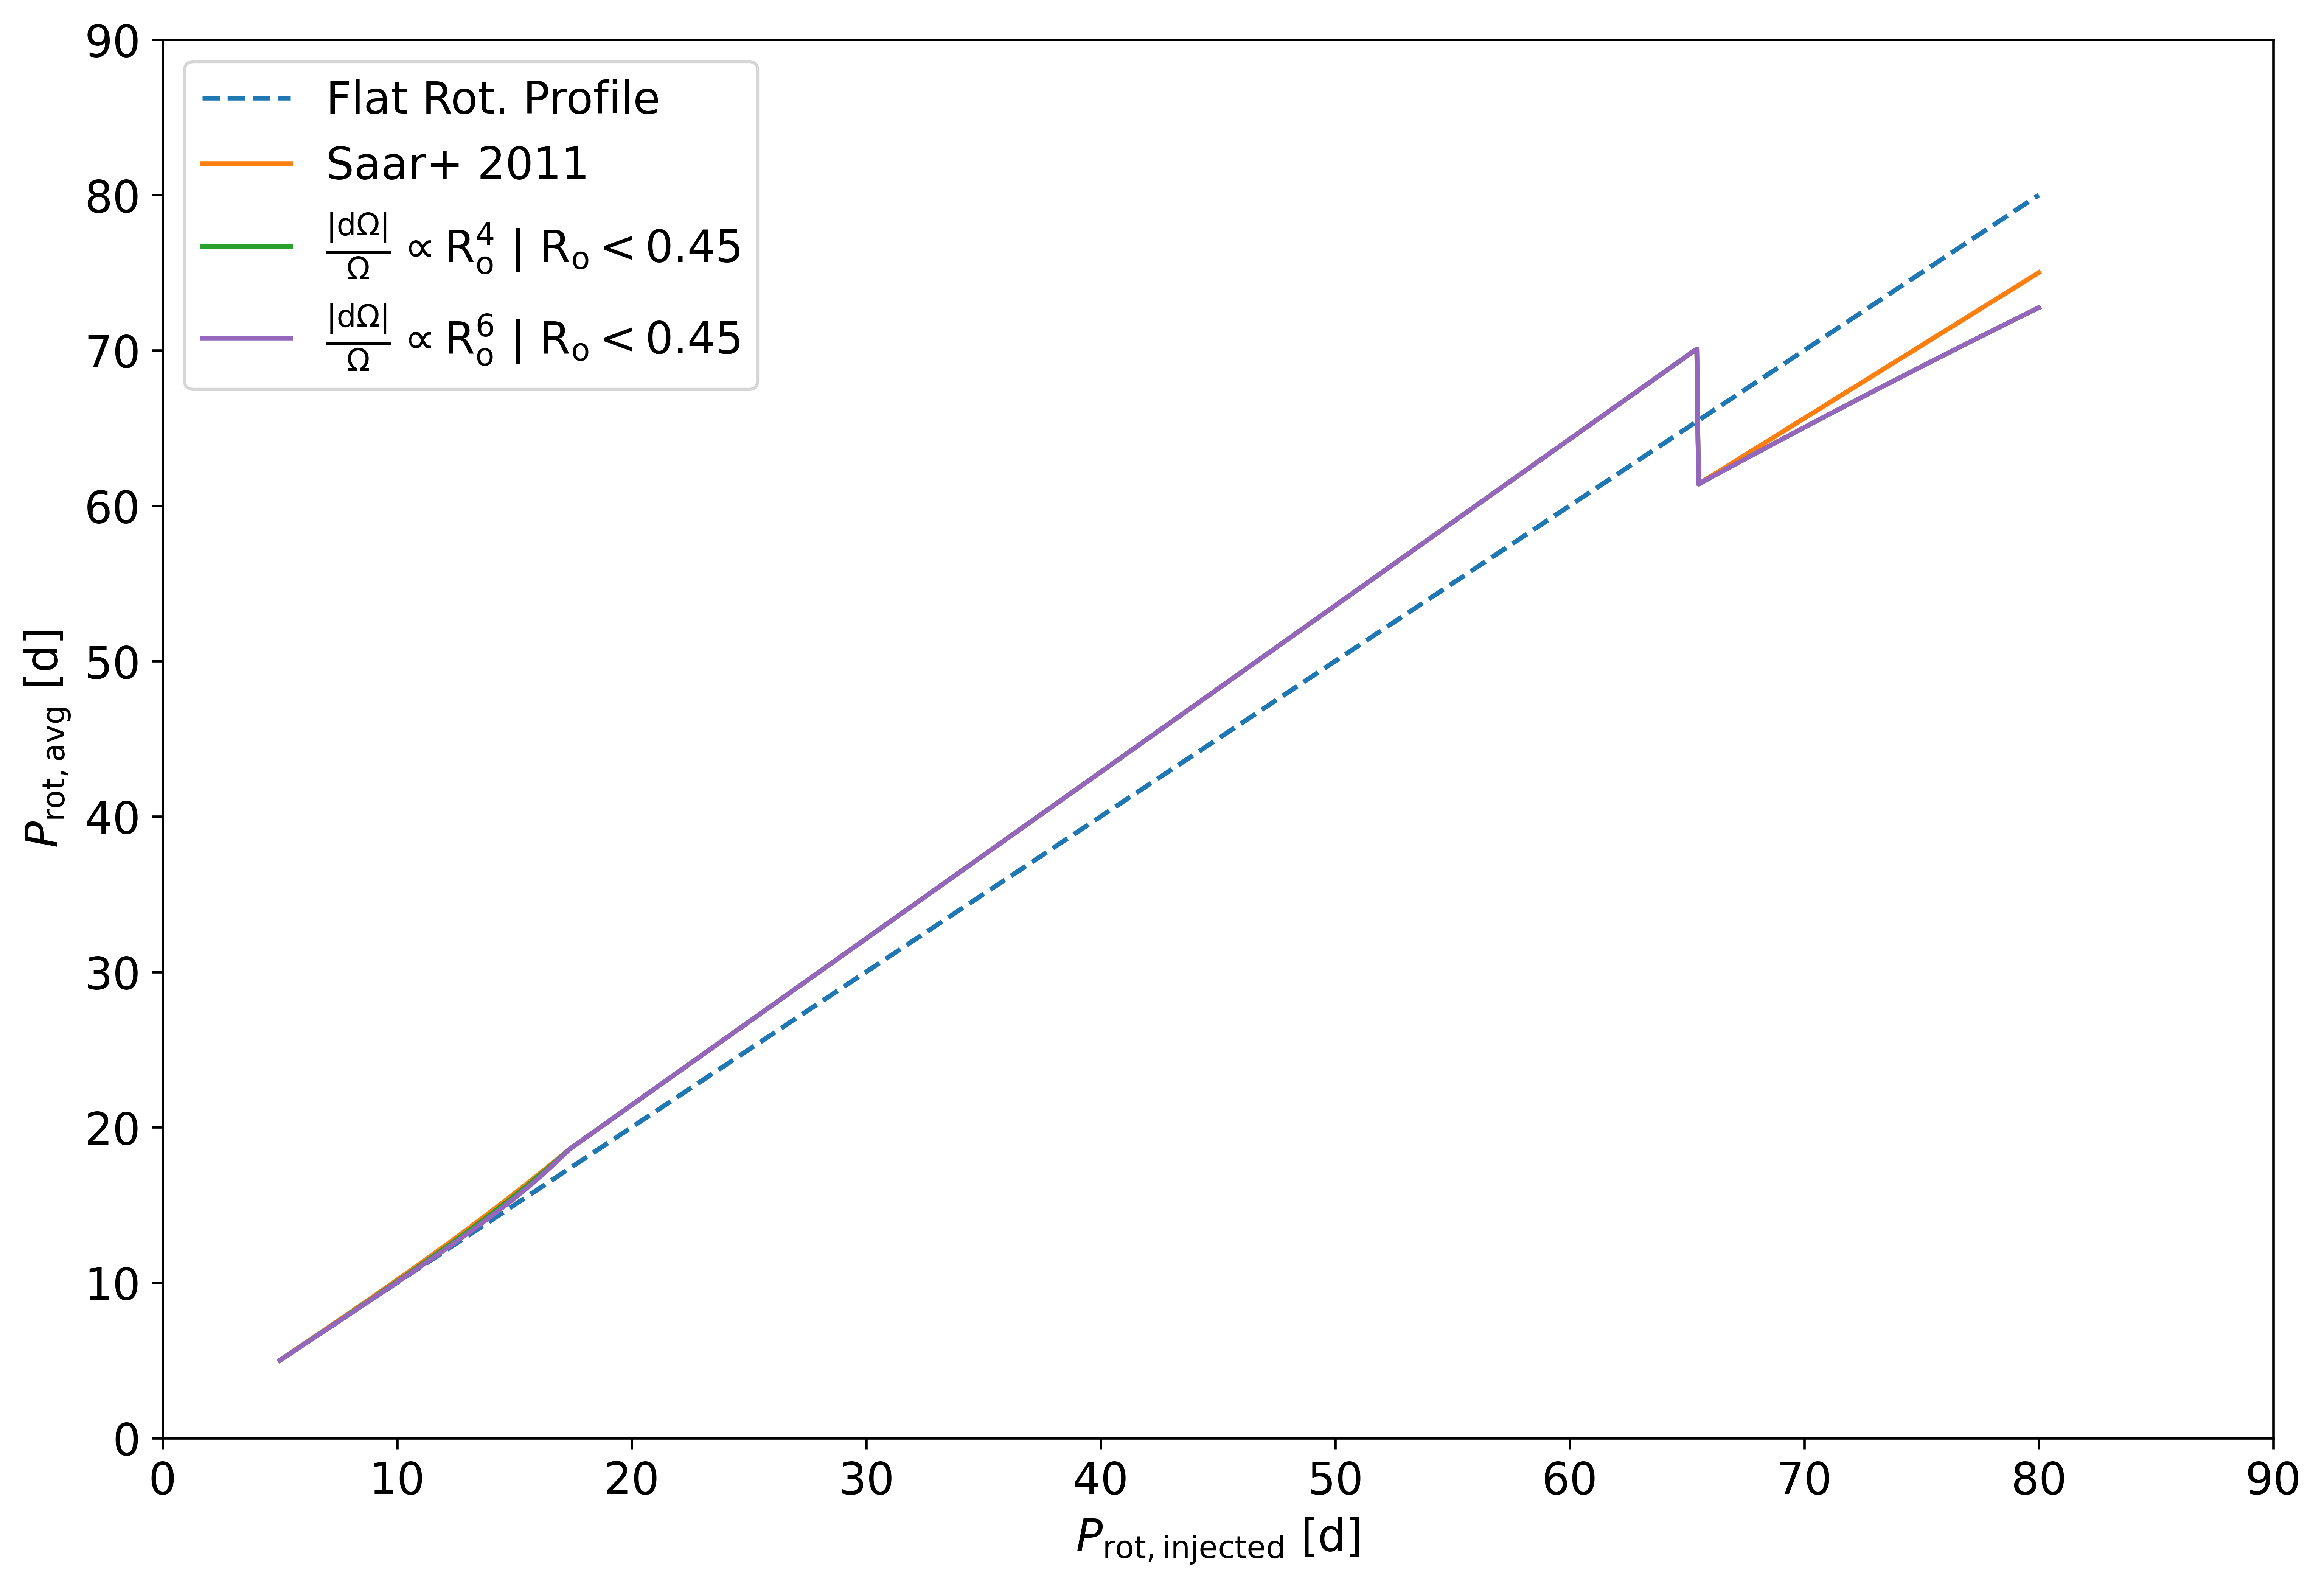
\includegraphics[width=\textwidth]{Figures/rot_gap_figures/comparison_observed_rot_periods.png}
 \caption[The effect of the differential rotation on the observed rotation period of a 0.7 $M_{\odot}$ against equatorial rotation period.]{
 	The effect of the differential rotation on the observed rotation period of a 0.7 $M_{\odot}$ star against the equatorial rotation period. Here, the colour of the relations corresponds to the adopted differential rotation relation in Figure \ref{fig:compar_diffrot} compared to the observed rotation profile of a latitudinally flat rotating star (blue), where the equatorial rotation period is the observed rotation period. At $R_o<0.45$ for injected rotation periods ($P_{\rm{eq}}$) less than 15 days, it is evident that steeper relations between $R_o$ and the scale of differential rotation lead to more rapid growth in observed rotation periods for the same equator rotation period. Moreover, a steeper growth in the observed rotation period corresponds to a lower number of observed stars with that particular rotation period. The transition from equator-fast to equator-slow rotation occurs at $P_{\rm{eq}} \ \sim \ 80$ days. The transition from the observed rotation period being greater than the equatorial rotation period results in a larger number of stars observed with similar rotation periods compared to the equator fast-regime \textbf{Inset:} The fractional period difference between the observed and equatorial rotation periods. The relation observed in this Figure is the same as is observed in Figure \ref{fig:compar_diffrot} but highlights the variance in the growth of the difference between the two steep relationships (green and purple) which is not visible when just comparing the observed and equatorial rotation periods. Despite being unable to differentiate between the two in this Figure, we will find that they introduce significant variations to the observed rotation period distribution.}
 \label{fig:comp_per}
\end{figure}

Now, we consider how the bias to rotation periods brought about by differential rotation has on the observed rotation period distribution.
To do this, we assume a sample of stars that are uniformly distributed in effective temperature $U\sim\left(3500,6000\right)$ and equatorial period $U\sim\left(0,55\right)$ days, where ${U}\sim \left(a,b\right)$ denotes a uniform prior between $a$ and $b$.
The bounds of these distributions are not physically motivated; they only need to include the regimes where $R_o \ = \ 0.45$ and $2$ to observe the effect that the transitions between latitudinally-flat, equator-fast, and equator-slow rotation have on the observed rotation period distribution.
We draw 100,000 effective temperatures and equatorial periods from these distributions and calculate the observed rotation periods under the adopted relationships between differential rotation and $R_o$ (Equations \ref{eq:rot_saar}, \ref{eq:rot_pow4}, and \ref{eq:rot_pow6}).
We plot the equatorial period and observed rotation periods under each of these relations as a 2D histogram in Figure \ref{fig:create_gap}.
We have also indicated in each panel the transitions between latitudinally-flat to significant equator-fast differential rotation (dashed line, $R_o = 0.45$), and equator-fast to equator-slow differential rotation (dashed line, $R_o = 2$).
Our models predict a dearth of observations, coincident with the intermediate period gap due to the transition from latitudinally flat to significant equator-fast differential rotation.
This can be seen by comparing the top left panel to the other three panels.
The distinctness, or rather the decrease in density of stars within the gap, increases with the power on $R_o$ (2, 4, and 8 for Equations \ref{eq:rot_saar}, \ref{eq:rot_pow4}, \ref{eq:rot_pow6} respectively) within the transition between latitudinally-flat to significant equator-fast differential rotation, $R_o \leq 0.45$.
We also find that our models predict an over-density of observations where the transition from equator-fast to equator-slow latitudinal differential rotation occurs ($P \ = \ 25$ d, $T_{\rm{eff}} \ = \ 6000 \ K$).

\begin{figure}
\centering
 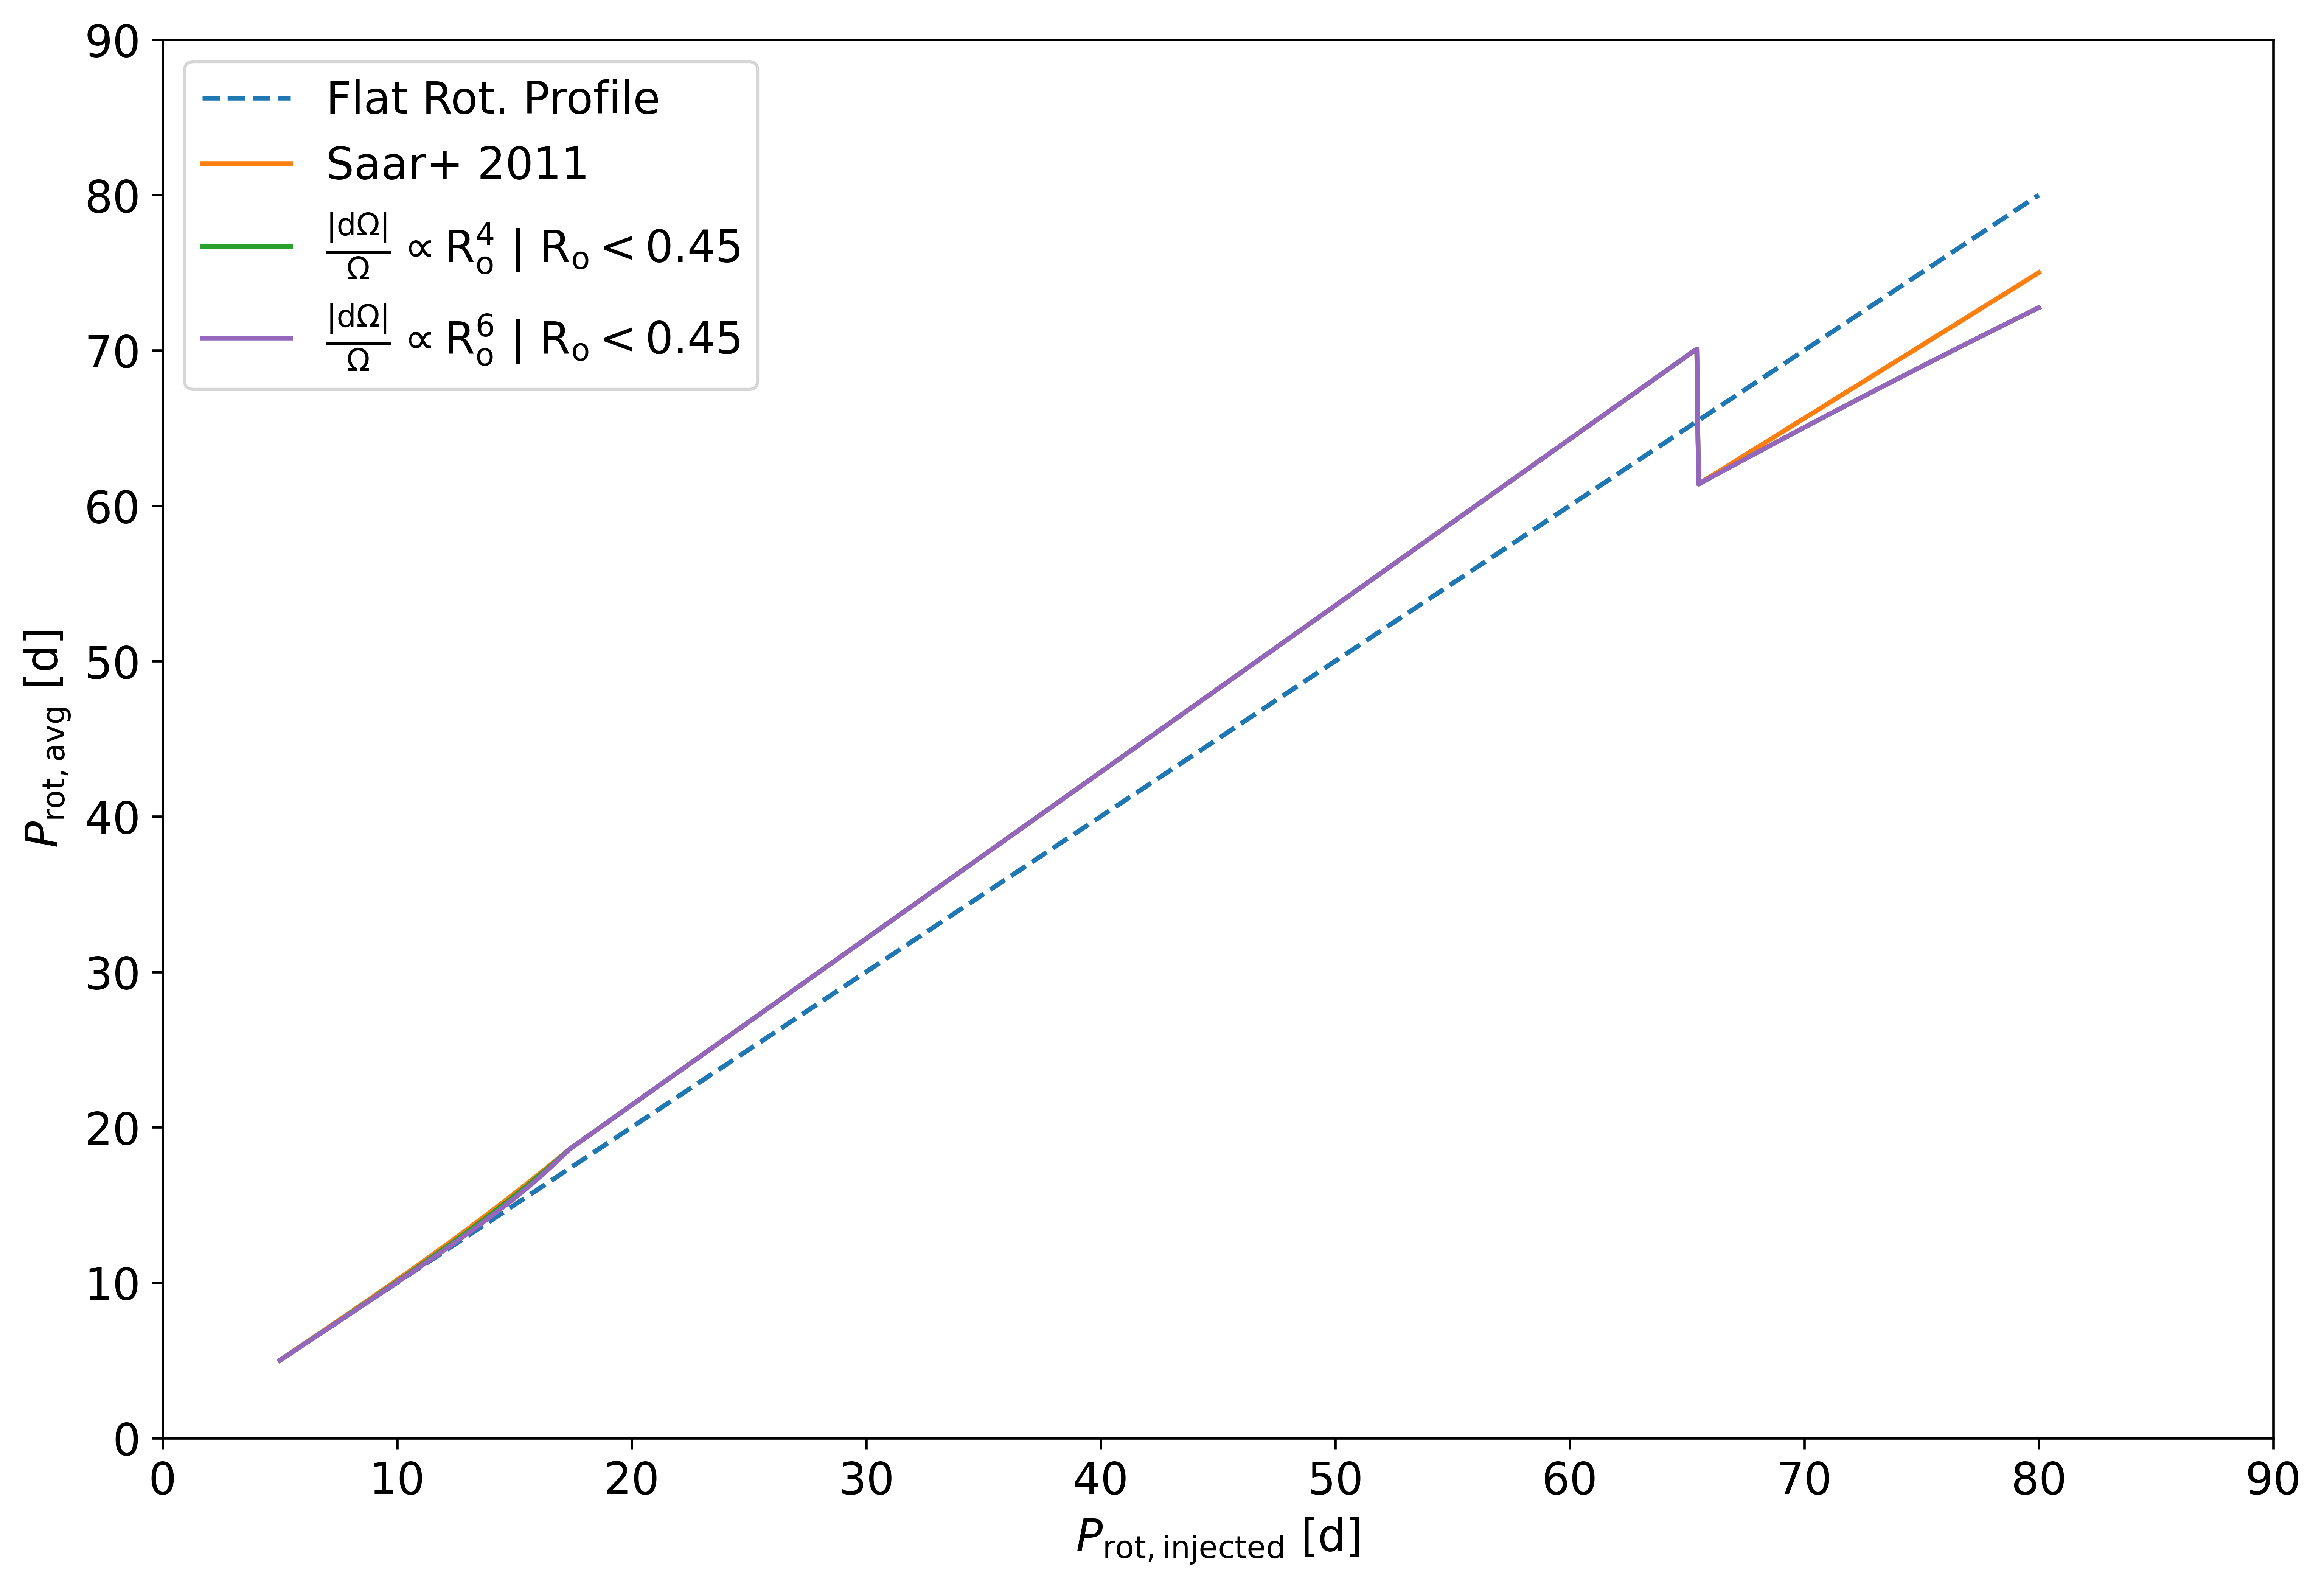
\includegraphics[width=\textwidth]{Figures/rot_gap_figures/comparison_observed_rot_periods.png}
 \caption[The effect of differential rotation on the observed rotation period distribution.]{The effect of differential rotation on the observed rotation period distribution of a sample of stars with uniformly distributed effective temperature and equatorial rotation period. We show the 2D histograms of the equatorial rotation period (top left) against effective temperature as well as the observed rotation periods under each of the adopted differential rotation relations: Equations \ref{eq:rot_saar} (top right), \ref{eq:rot_pow4} (bottom left), and\ref{eq:rot_pow6} (bottom right). The transitions between latitudinally-flat to significant equator-fast differential rotation ($R_o = 0.45$), and equator-fast to equator-slow differential rotation ($R_o = 2$) are shown in dashed and dotted lines, respectively. Our models predict a dearth of observations, coincident with the intermediate period gap due to the transition from latitudinally flat to significant equator-fast differential rotation and an over-density of observations at the transition from equator-fast to equator-slow rotation.}
 \label{fig:create_gap}
\end{figure}

\subsection{A physically motivated synthetic sample of observed rotation periods}

We require a physically motivated synthetic sample of rotation periods to compare our model to the observed rotation period distribution of \citet{mcquillan_rotation_2014}.

We adopt equatorial rotation periods ($P_{\rm{eq}}$) from cluster-tuned rotational isochrones for a given stellar age and mass (these rotational isochrones are shown in Table A1 in \citet{spada_competing_2020}).
The ages of these isochrones are limited to the solar age (4.5 Gyr), placing an upper limit on the age of our population.

The use of their rotation periods in this work warrants some discussion.
In their work, they propose a model of rotation period evolution that a wind braking and 2-zone (core and surface) mass-dependent angular momentum transport.
They tune the wind-braking and core-envelope coupling timescale through the measured rotation periods of young clusters: Pleiades (120 Myr, \citep{rebull_rotation_2016}), Praesepe (700 Myr, \citep{douglas_poking_2017, douglas_k2_2019}), and NGC 6811 (1 Gyr, \citep{curtis_temporary_2019}) as well as the rotation period of the Sun (4.5 Gyr).
The adopted rotation period of the Sun in their work is also the scaled average rotation period of the latitudinally differentially rotating surface scaled by the latitudinal distribution of stellar spots rather than the equatorial rotation period (26.9 d).
This value is notably much closer to the equator rotation period ($\sim 25$ d) than the polar rotation period ($\sim 31$ d) of the Sun.

If, indeed, we are correct that latitudinal differential rotation introduces biases to the measured rotation period, then tuning models using measured rotation periods and not accounting for the bias (that latitudinal differential rotation may introduce) could result in inaccurate prescriptions of the evolution of rotation.
The measured rotation periods used to tune our generative model of what we assume are equatorial rotation periods are shown in Figure \ref{fig:com_gap_clus}.
We have also plotted the line $R_o \ = \ 0.45$, where we assume equator-fast latitudinal differential rotation becomes significant and, therefore, impacts the observed rotation period.
We observe that a majority of high-temperature ($>$ 5000 K) Pleiades and Praesepe members lay above this line.
This suggests that the measured rotation periods of high-mass stars in their work are not equatorial but, in fact, already the biased, measured rotation periods.
We will be introducing a bias to potentially already biased rotation periods for high-mass stars in our sample.
On the other hand, low-mass stars ($>$ 5000 K) lay below this line.
This suggests that the measured rotation period of these low-mass stars is the equatorial rotation period and that the model is tuned to only the equatorial rotation periods of low-mass stars.
Older ($>$ 1 Gyr) low-mass rotation periods output by their model are projections of the equator-tuned rotation periods under their model.
Given that the introduced dearth is most apparent for low-mass stars older than 1 Gyr, we believe adopting these values as the equatorial rotation periods is appropriate.

We also compare in this Figure the rotation period distributions of each cluster against the rotation periods of the \citet{spada_competing_2020} model evaluated at the representative ages of each of the clusters (dashed lines).
While this model generally agrees with the high-mass members of the clusters, it was tuned to (Pleiades, Praesepe, NGC 6811), as well as the high-mass members of NGC 6819, it significantly over-predicts the rotation periods of low-mass stars.
This is especially pervasive for stars with effective temperatures less than 4000 K.
This results in very few low-mass stars with rotation periods that place them on the lower branch of the intermediate period gap and an over-density of observed rotation periods of low-mass stars.
We, therefore, exclude stars with effective temperatures less than 4000 K from our synthetic sample. 
While this leaves us with a small range of effective temperatures that we adopt in our work, where the model rotation period is the equatorial rotation period, the gap is still apparent in this range: we are able to see, qualitatively, if the bias introduced by differential rotation produces a gap consistent with the observed rotation periods.
We will revisit this assumption in reference to our conclusions in Section \ref{sec:discussion}.

\begin{figure}
\centering
 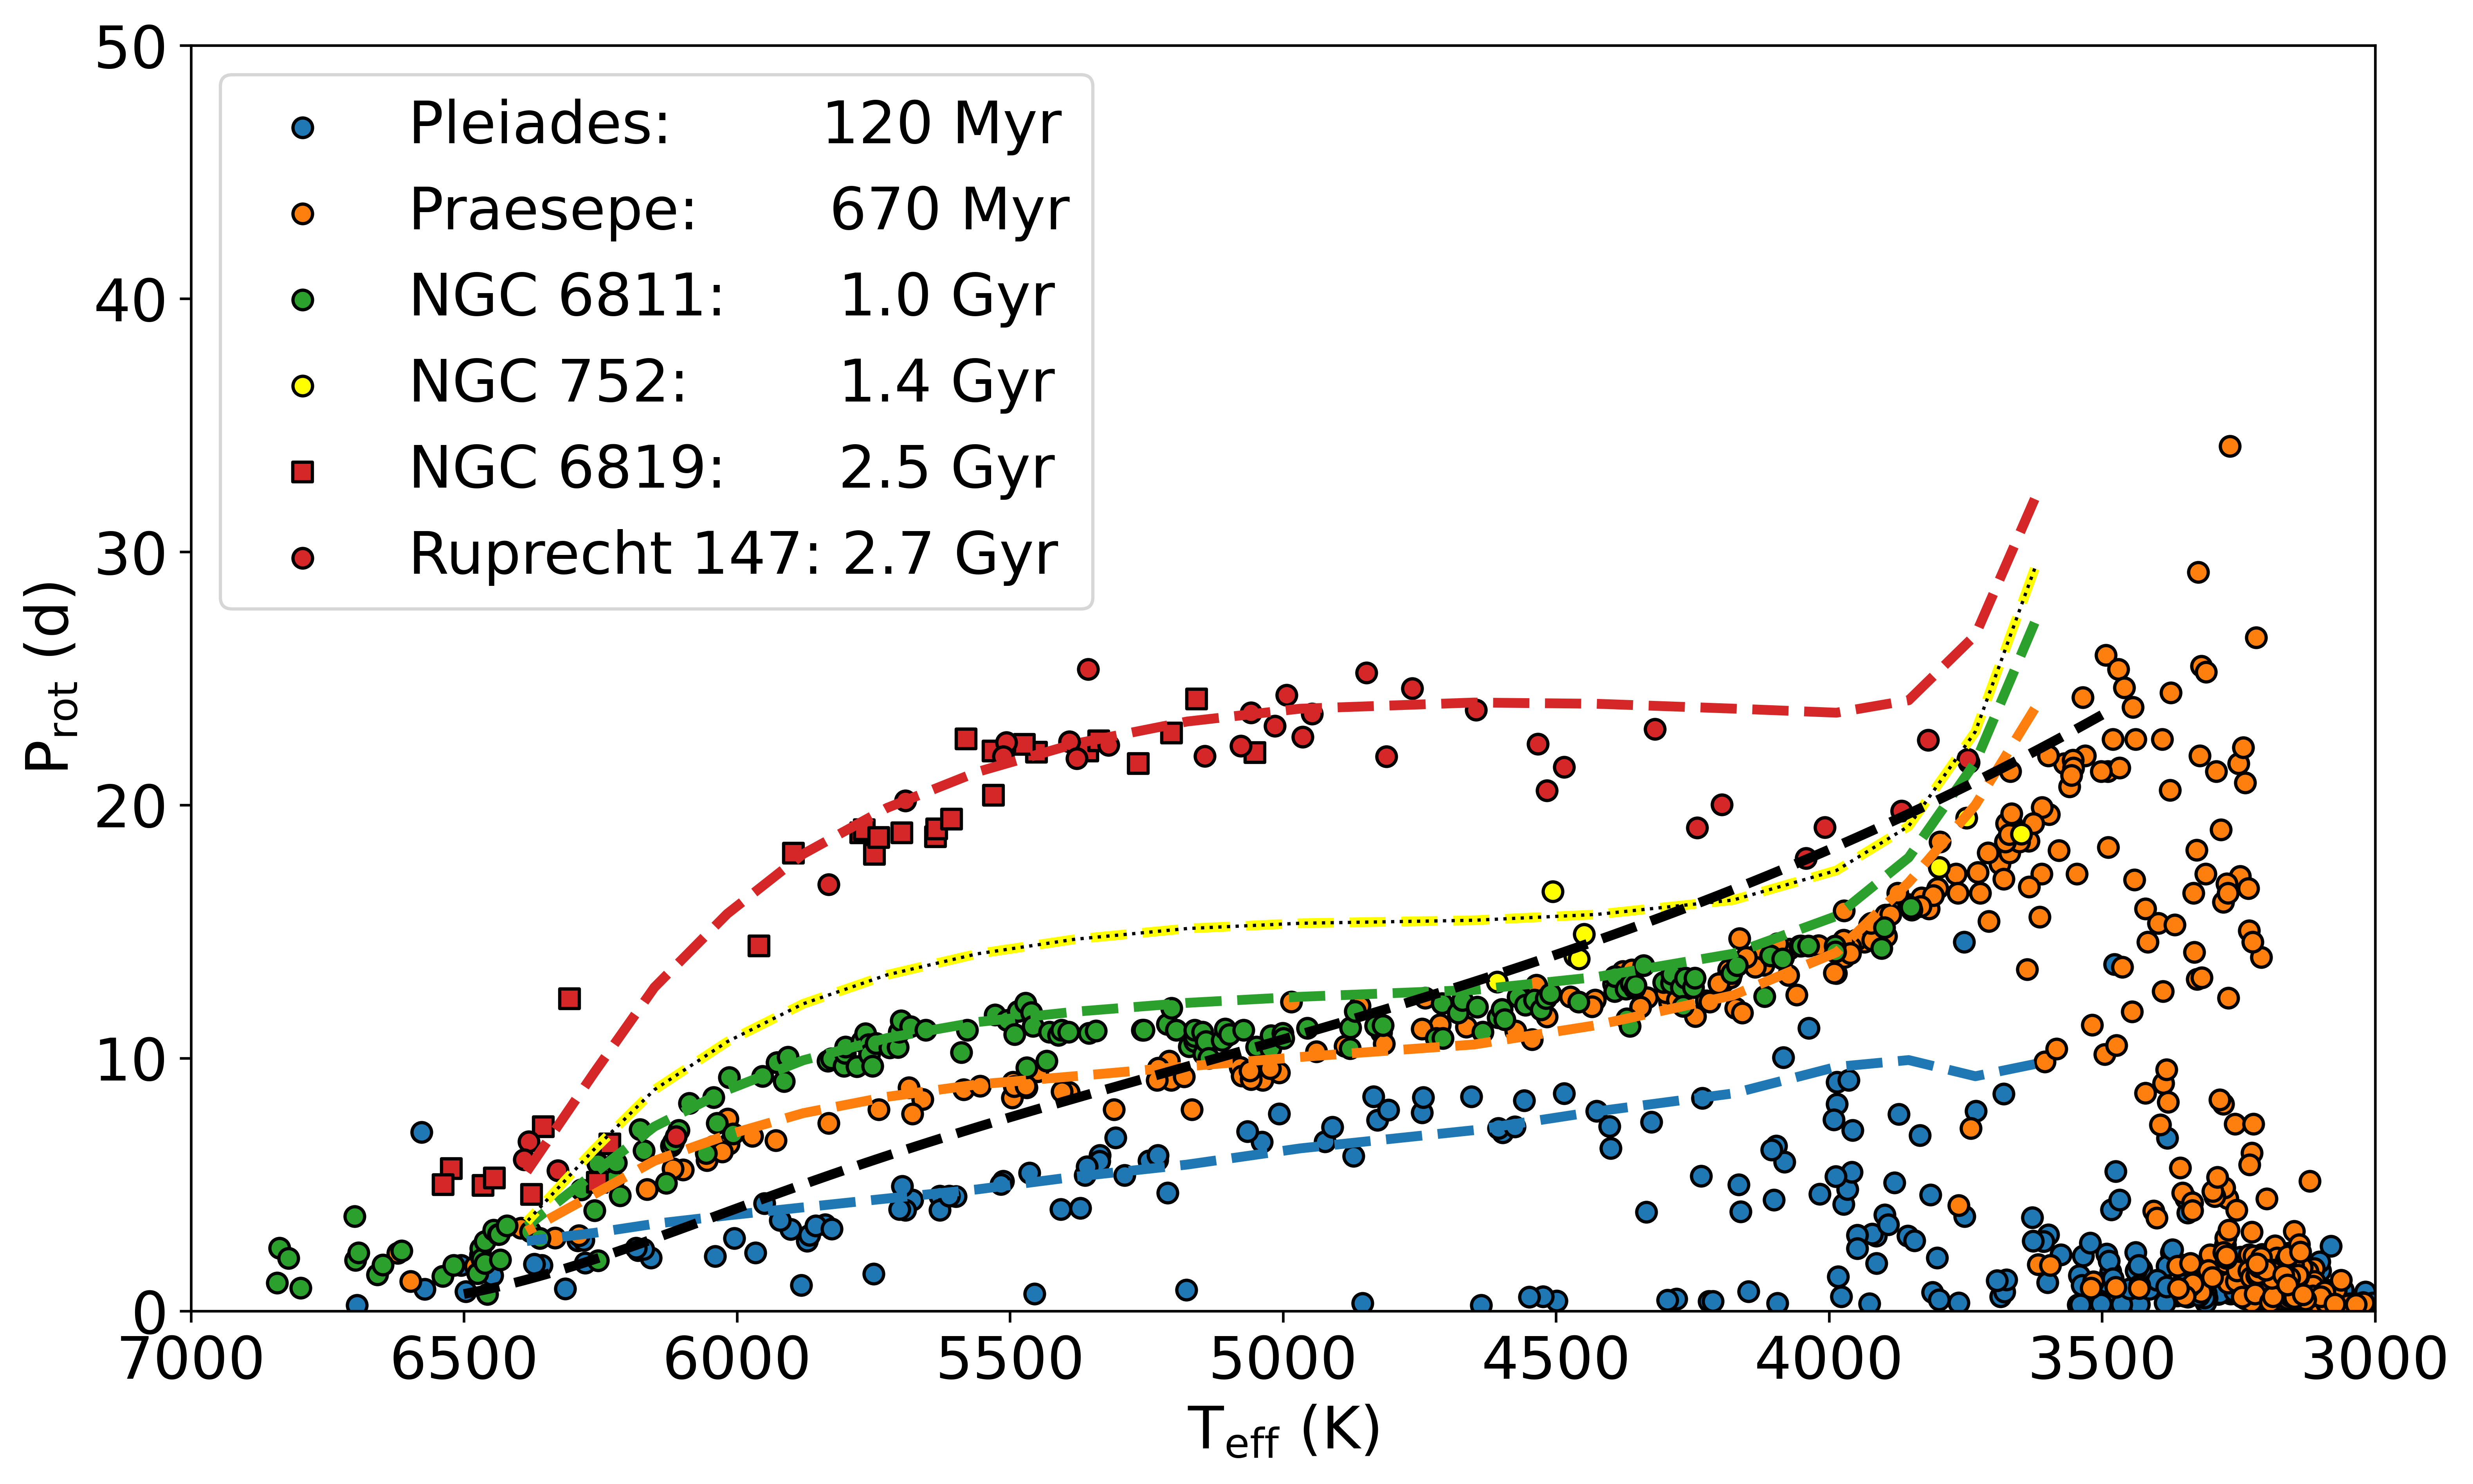
\includegraphics[width=\textwidth]{Figures/rot_gap_figures/com_gap_clus.png}
 \caption[Cluster rotation periods distributions against effective temperature.]{Scatter plot of clusters, Pleiades (120 Myr, blue \citep{rebull_rotation_2016}), Praesepe (orange, 700 Myr, \citep{douglas_poking_2017, douglas_k2_2019}) and NGC 6811 (green, 1 Gyr, \citep{curtis_temporary_2019}), used to tune the rotational isochrones adopted in this work \citep{spada_competing_2020} as well as the rotational period distributions of NGC 752 (yellow, 1.4 Gyr), NGC 6819 (red squares, 2.5 Gyr - projected forward to 2.7 Gyr: scaled through Skumanich spin-down, for direct comparison with the Ruprecht 147 sample, \citep{meibom_kepler_2011}), and Ruprecht 147 (red circles, 2.7 Gyr, \citep{curtis_when_2020}) against effective temperature. \textbf{Dashed lines:} \citep{spada_competing_2020} rotational isochrones evaluated at the ages of each stellar cluster and coloured to match the scatter points. We have also shown the line $R_o \ = \ 0.45$ in black, highlighting that the high temperature ($\>$5000K) Pleiades and Praesepe members may have significant latitudinal differential rotation, biasing the observed rotation periods, while low-temperature stars may not. Suggesting that the observed rotation period of these stars is the equatorial rotation period, and adopting the \citet{spada_competing_2020} values as the equator rotation periods is appropriate for low-mass stars. We also show the rotation periods evaluated by the \citet{spada_competing_2020} model evaluated at the representative ages of each cluster (dashed lines coloured by the cluster of the same age).
While this model generally agrees with the high-mass members of the clusters, it was tuned to (Pleiades, Praesepe, NGC 6811), as well as the high-mass members of NGC 6819, it significantly over-predicts the rotation periods of low-mass stars.
This is especially pervasive for stars with effective temperatures less than 4000 K.}
 \label{fig:com_gap_clus}
\end{figure}

%add references to the cluster rotation periods and discuss the discrepancy between the observed NGC6811 and Ruprecht 147 rotation periods. 


We generate 30,000 main-sequence and early post-main-sequence stars with various mass, age, metallicity and rotation rate values.
We drew masses from a uniform mass function $U\sim\left(0.65,1\right)$ $M_{\odot}$.
This limits our range of masses to those with a convective surface and radiative core and an effective temperature greater than 4000 K.
The gap is apparent in this range ($T_{\rm{eff}} \ < \ 5000$ K).
The choice of a uniform initial mass function here is motivated by the selection function of the \kepler\ mission being biased towards the observation of brighter stars.
We assume that the selection function effectively cancels out the bias towards a larger number of low-mass stars of physically motivated initial mass functions like a Salpeter initial mass function.

%todo:check this with Andy
Metallicity is drawn from a distribution to approximately reflect what is observed in the Milky Way. Specifically, we defined a variable $\phi$ to be drawn from a Beta distribution
\begin{equation}
 \phi \sim \mathcal{B}\left(\alpha=10, \beta=2\right)
\end{equation}
and applied a transform from $\phi$ to [Fe/H] by requiring the metallicities be bounded between $[\mathrm{Fe/H}]_\mathrm{min} =-2$ and $[\mathrm{Fe/H}]_\mathrm{max} = +0.5$. We also required that the mode of $\phi$, defined as $\frac{\alpha - 1}{\alpha + \beta - 2}$ for a Beta distribution, occurs at Solar metallicity. This leads to the transform:
\begin{equation}
 [\mathrm{Fe/H}] = \left(\frac{}{}[\mathrm{Fe/H}]_\mathrm{max}-[\mathrm{Fe/H}]_\mathrm{min}\right)\left(\phi - \frac{\alpha - 1}{\alpha + \beta - 2}\right) \quad .
\end{equation}

The stars we generate mock data for in this work span from the ZAMS to low-luminosity subgiants.
We draw equivalent evolutionary phase (EEP) values\footnote{The principle of the EEPs is to define physically significant stages in stellar evolution (e.g. core-H burning, core-H depletion, RGB), and then subdivide each of these stages into a number of equal steps. See \citet{morton_isochrones_2015} for a more in-depth discussion of the definition of these values.} from a uniform distribution of EEPs $U\sim(200,450)$.
The bounds of this range (200 and 450) represent the zero-age-main-sequence and the low-luminosity subgiant phase, respectively.
Using the EEP, mass, and metallicity, we interpolate a position along the MIST stellar isochrones \citep{morton_isochrones_2015} to calculate the expected \teff \ , and luminosity of each star as well as the post-zero-age main-sequence age.
This results in a population biased towards younger ($<$ 1 Gyr) stars.
We found that after calculating the equator rotation periods under this population the rotational period distribution had a much higher density of observations of low rotational periods than the \citet{mcquillan_rotation_2014} sample, ensuring comparison between the two is not biased by the choice of age distribution.
We therefore sampled our population until we had a population uniform in age between 300 Myr and 4.5 Gyr, ensuring the sample was on the slow-rotator sequence but younger than the solar age.
From these parameters, we can then calculate the observed rotation periods of our synthetic sample.

\section{Results}
\label{sec:results}

The resulting distributions of stars (blue, orange, green and purple) relative to the observed distribution of \kepler{} rotation periods measured in \citet{mcquillan_rotation_2014} (black) are shown in Figure \ref{fig:comp_dist}.
Here, the colour of each distribution corresponds to the same colour, showing the relation between differential rotation and $R_o$ in Figure \ref{fig:compar_diffrot} and blue corresponds to the equatorial, or latitudinally-flat rotation profile observed, rotation period.

Figure \ref{fig:comp_hess} shows how the adopted relations impact the rotation period distributions.
The left column shows the 2D histogram of the \citet{mcquillan_rotation_2014} rotation period distribution.
In the middle column, we show the 2D histogram of the observed rotation period distributions under the adopted relations between latitudinal differential rotation and $R_o$.
From top to bottom panel, we show the injected rotation periods from our generative model (with no latitudinal differential rotation), then under the \citet{saar_starspots_2011} Equation (\ref{eq:rot_saar}) differential rotation relation, then with the Equation (\ref{eq:rot_pow4}) model, and finally with the Equation (\ref{eq:rot_pow6}) model.
These panels correspond to the blue, orange, green, and purple distributions in Figure \ref{fig:compar_diffrot} respectively.
All of the panels in the left two columns are coloured by the number of stars in each bin for each panel.
N$_{\rm{Obs.}}$, the number in each bin of the \citet{mcquillan_rotation_2014} sample, for the left column and N$_{\rm{Mod.}}$, the number in each bin of the various models, for the middle column.
In the right column, we show the difference between the distributions through N$_{\rm{Obs.}}$ and N$_{\rm{Mod.}}$ for each adopted relation.
Darker colours correspond to regions where the model over-predicts observations and lighter where the model under-predicts observations.

Like in Figure \ref{fig:create_gap}, our models predict a dearth of observations, coincident with the intermediate period gap as a result of the transition from latitudinally flat to equator-fast differential rotation at $R_o = 0.45$.
We observe that the model that adopts latitudinal differential rotation when calculating the observed rotation period reduces the disparity between the model and observed rotation period distributions.
This can be seen comparing the top panel to the bottom three in the right column of Figure \ref{fig:comp_hess}.
Further, the increased density of observations of stars just above the intermediate period gap in the \kepler{} sample is reproduced under this model, unlike a model of extreme magnetic braking to explain the gap.
We again observe that increases with the power on $R_o$ (2, 4, and 8 for Equations \ref{eq:rot_saar}, \ref{eq:rot_pow4}, \ref{eq:rot_pow6} respectively) increase the distinctiveness (relative decrease in density of observations) of the gap.
We also find that all models predict an over-density of stars where the transition from equator-fast to equator-slow latitudinal differential rotation occurs ($\log P_{\rm{rot}}/d = 1.2$, $T_{\rm{eff}} = 6000 \ K$), coinciding with the long-period pileup.
The model also predicts this over-density with no differential rotation, but the shape of the distributions in this domain do not agree.
When we introduce differential rotation, however, the shape of the upper edge of the model rotation period distribution closely matches the shape of the measured rotation period distribution.
Suggesting that the cause of the long-period pileup is this transition.

\begin{figure}
\centering
 \includegraphics[width=\textwidth]{Figures/rot_gap_figures/comp_dist.png}
 \caption[The observed rotation period distributions of the synthetic sample of stars given various relations between latitudinal differential rotation and $R_o$ overlayed over the observed distribution of rotation periods of the \kepler{} sample from \citet{mcquillan_rotation_2014} (black).]{
 	The observed rotation period distributions of the synthetic sample of stars given various relations between latitudinal differential rotation and $R_o$ overlayed over the observed distribution of rotation periods of the \kepler{} sample from \citet{mcquillan_rotation_2014} (black). Here, the coloured observed rotation period distributions correspond to the various differential rotation relations adopted in this work, as seen in Figure \ref{fig:compar_diffrot}. The latitudinally flat (blue, top left) sample reflects the equatorial rotation periods of our sample considered in this work. We observe no intermediate period gap in this synthetic sample of stars without differential rotation. 
We also see signs that if we include the effects of differential rotation on the observed rotation period, a dearth of observations at the transition between latitudinally flat ($R_o \ < \ 0.45$) and equator-fast rotation occurs precisely at the location of the intermediate period gap.
Further, we observe that as the steepness of the scale of differential rotation with $R_o$ for $R_o \ < \ 0.45$ increases (where in order of increasing steepness, we have the orange, green and purple distributions, corresponding to Equations \ref{eq:rot_saar}, \ref{eq:rot_pow4}, \ref{eq:rot_pow6} respectively) the gap becomes more distinct - fewer stars are observed within the gap. 
We also find that due to the transition from equator-fast to anti-equator-fast differential rotation, we obtain a potential over-density of stars consistent with the over-density of slow-rotating stars near 6000 K.
While we can see signs of the effect of differential rotation on the observed rotation periods, the rotation period distribution is not well reflected in this Figure. We have plotted the 2D histograms of these distributions to qualify and make comparisons between the observed and modelled rotation distributions in Figure \ref{fig:comp_hess}.}
 \label{fig:comp_dist}
\end{figure}

\begin{figure}
\centering
 \includegraphics[width=\textwidth]{Figures/rot_gap_figures/comp_hess_up.png}
 \caption[2D histograms of observed and the synthetic observed rotation period distribution assuming various relations between the scale of differential rotation and $R_o$ and the difference between the two.]{
2D histograms of observed and the synthetic observed rotation period distribution assume various relations between the scale of differential rotation and $R_o$ and the difference between the two.
\textbf{Left:} 2D histogram of the \citet{mcquillan_rotation_2014} rotation period distribution.
\textbf{Middle:} 2D histogram of the observed rotation period distributions under the adopted relations between latitudinal differential rotation and $R_o$. From top to bottom panel, we show the injected rotation periods from our generative model (with no latitudinal differential rotation), then the relation under the \citet{saar_starspots_2011} differential rotation relation (Equation \ref{eq:rot_saar}), then with two steeper but physically probable (Equation \ref{eq:rot_saar}) and two model motivated \citep{brun_powering_2022} scale of differential rotation relations Equations \ref{eq:rot_pow4}, \ref{eq:rot_pow6}.
These distributions correspond to the blue, orange, green, and purple distributions in Figure \ref{fig:compar_diffrot} respectively.
All of the panels in the two left columns are colour by the number of stars in each bin: N$_{\rm{Obs.}}$ for the left column and N$_{\rm{Mod.}}$ for the middle.
N$_{\rm{Obs.}}$, the number in each bin of the \citet{mcquillan_rotation_2014} sample, for the left column and N$_{\rm{Mod.}}$, the number in each bin of the various models, for the middle column.
\textbf{Right:} The difference between the distributions: N$_{\rm{Obs.}}$ - N$_{\rm{Mod.}}$ for each adopted relation.
Darker colours correspond to regions where the model over-predicts observations and lighter where the model under-predicts observations. We observe that the accounting for differential rotation when determining the expected observed rotation periods of stars introduces a decrease in the density of observations where significant differential rotation arises (here at $R_o \sim 0.45$). This dearth is coincident with the observed intermediate period gap. We find that the larger the power in the relation between $\frac{\Delta\Omega}{\Omega_{\rm{eq}}}$ and $R_o$ below the transition to a saturated scale of differential rotation (2, 4, and 8 for Equations \ref{eq:rot_saar}, \ref{eq:rot_pow4}, \ref{eq:rot_pow6} respectively), the more apparent the dearth becomes. We also find that our models predict an over-density of stars where the transition from equator-fast to equator-slow latitudinal differential rotation occurs ($\log P_{\rm{rot}/days} \ = \ 1.2$, $T_{\rm{eff}} \ = \ 6000$ K) corresponding with the position of the long-period pileup.}
 \label{fig:comp_hess}
\end{figure}

\section{Discussion}
\label{sec:discussion}

In this Chapter, we have proposed a novel explanation for the intermediate period gap: the growth equator-fast differential rotation near the location of the intermediate period gap and the effect that this has on the observed rotation periods of stars.
We propose this explanation for the intermediate period gap due to our perceived lack of evidence for other current explanations for the intermediate period gap.
Those two leading theories are that stars in the intermediate period gap drop below the detectability threshold suggested by the drop in photometric variability of stars near the gap or that stats "jump" the intermediate period gap through sudden enhanced magnetic braking.
In Appendix \ref{apndx:magnetic} of this thesis, we have discussed an investigation into evidence against these explanations, which we believe suggests that these explanations are not the underlying mechanism of the intermediate period gap.

In this work, we consider the effect of latitudinal differential rotation on the observed rotation periods of main-sequence stars.
To do this, we developed a model to predict the observed/average rotation period of stars given models of surface latitudinal differential rotation growth from observational and 2D magnetohydrodynamical simulations of rotating main-sequence stars.
The observations of latitudinal differential rotation and magnetohydrodynamical models of latitudinal differential rotation with $R_o$ agree - suggesting that latitudinal differential rotation grows from latitudinally flat to equator-fast differentially rotating at a $R_o \approx 0.45$.
Introducing this differential rotation to our calculation of the average surface rotation period of stars produces a lower density of observations where the differential rotation grows.
We believe that this suggests that the underlying mechanism of the intermediate period gap is the onset of latitudinal differential rotation.
We have investigated several relationships between the scale of growth of latitudinal differential rotation and $R_o$. The qualitatively best-fit relations have a swift growth of $\frac{\Delta\Omega}{\Omega_{\rm{eq}}}$ close to the intermediate period gap (Equations \ref{eq:rot_pow4} and \ref{eq:rot_pow6}).
We found in this work the distinctness, or rather the decrease in density of stars within the gap, increases with the power on $R_o$ when $R_o \leq 0.45$.

While our model predicts a dearth of observations coincident with the gap, we are hesitant to suggest a prescription for the growth of the scale of differential rotation based on our results.
There is significant degeneracy between several parameters in our work, and there are still many unknowns that we have yet to account for that require future work.

We adopt a constant distribution of stellar spots between a latitude of $0^{\circ}$ and $60^{\circ}$.
The evolution of the latitudinal distribution of stellar spots is unknown, so we will not speculate as to whether changes to this parameter would result in our models reflecting the observed rotational distribution.
However, we will note the effects that variations to this parameter have.
If spots are more concentrated to the equator ($\theta_{\rm{min}} = 0^{\circ}$ and $\theta_{\rm{max}} < 60^{\circ}$) then the observed rotation periods more closely reflect the equator/injected rotation periods.
Conversely, if spots are more concentrated toward the poles ($\theta_{\rm{min}} > 0^{\circ}$ and $\theta_{\rm{max}} > 60^{\circ}$), then differential rotation will have a larger effect on the observed rotation periods.
The variations that those variations make are similar to an increase in the saturated scaling of differential rotation $\left(\frac{\Delta\Omega}{\Omega_{\rm{eq}}}\right)$.
The larger this value, the greater the scale of the dearth region in terms of rotation period.

We have adopted a uniform function to draw our stellar masses.
A uniform mass distribution better reflects the mass distribution of the \citet{mcquillan_rotation_2014} sample (a Salpeter initial mass function, for example, predicts an order of magnitude greater number of low-mass stars), but under-predicts the number of high-mass stars relative to low-mass stars.
The probability density distributions generally agree when comparing the effective temperature and luminosity distributions, as seen in Figure \ref{fig:compar_teff_logl}.
We believe that this assumption is sound.
The relative distribution of rotational periods and effective temperatures between the two distributions (observed and modelled), as we have performed in Section \ref{sec:results}, will therefore not be significantly biased by the underlying mass distribution.

\begin{figure}
\centering
 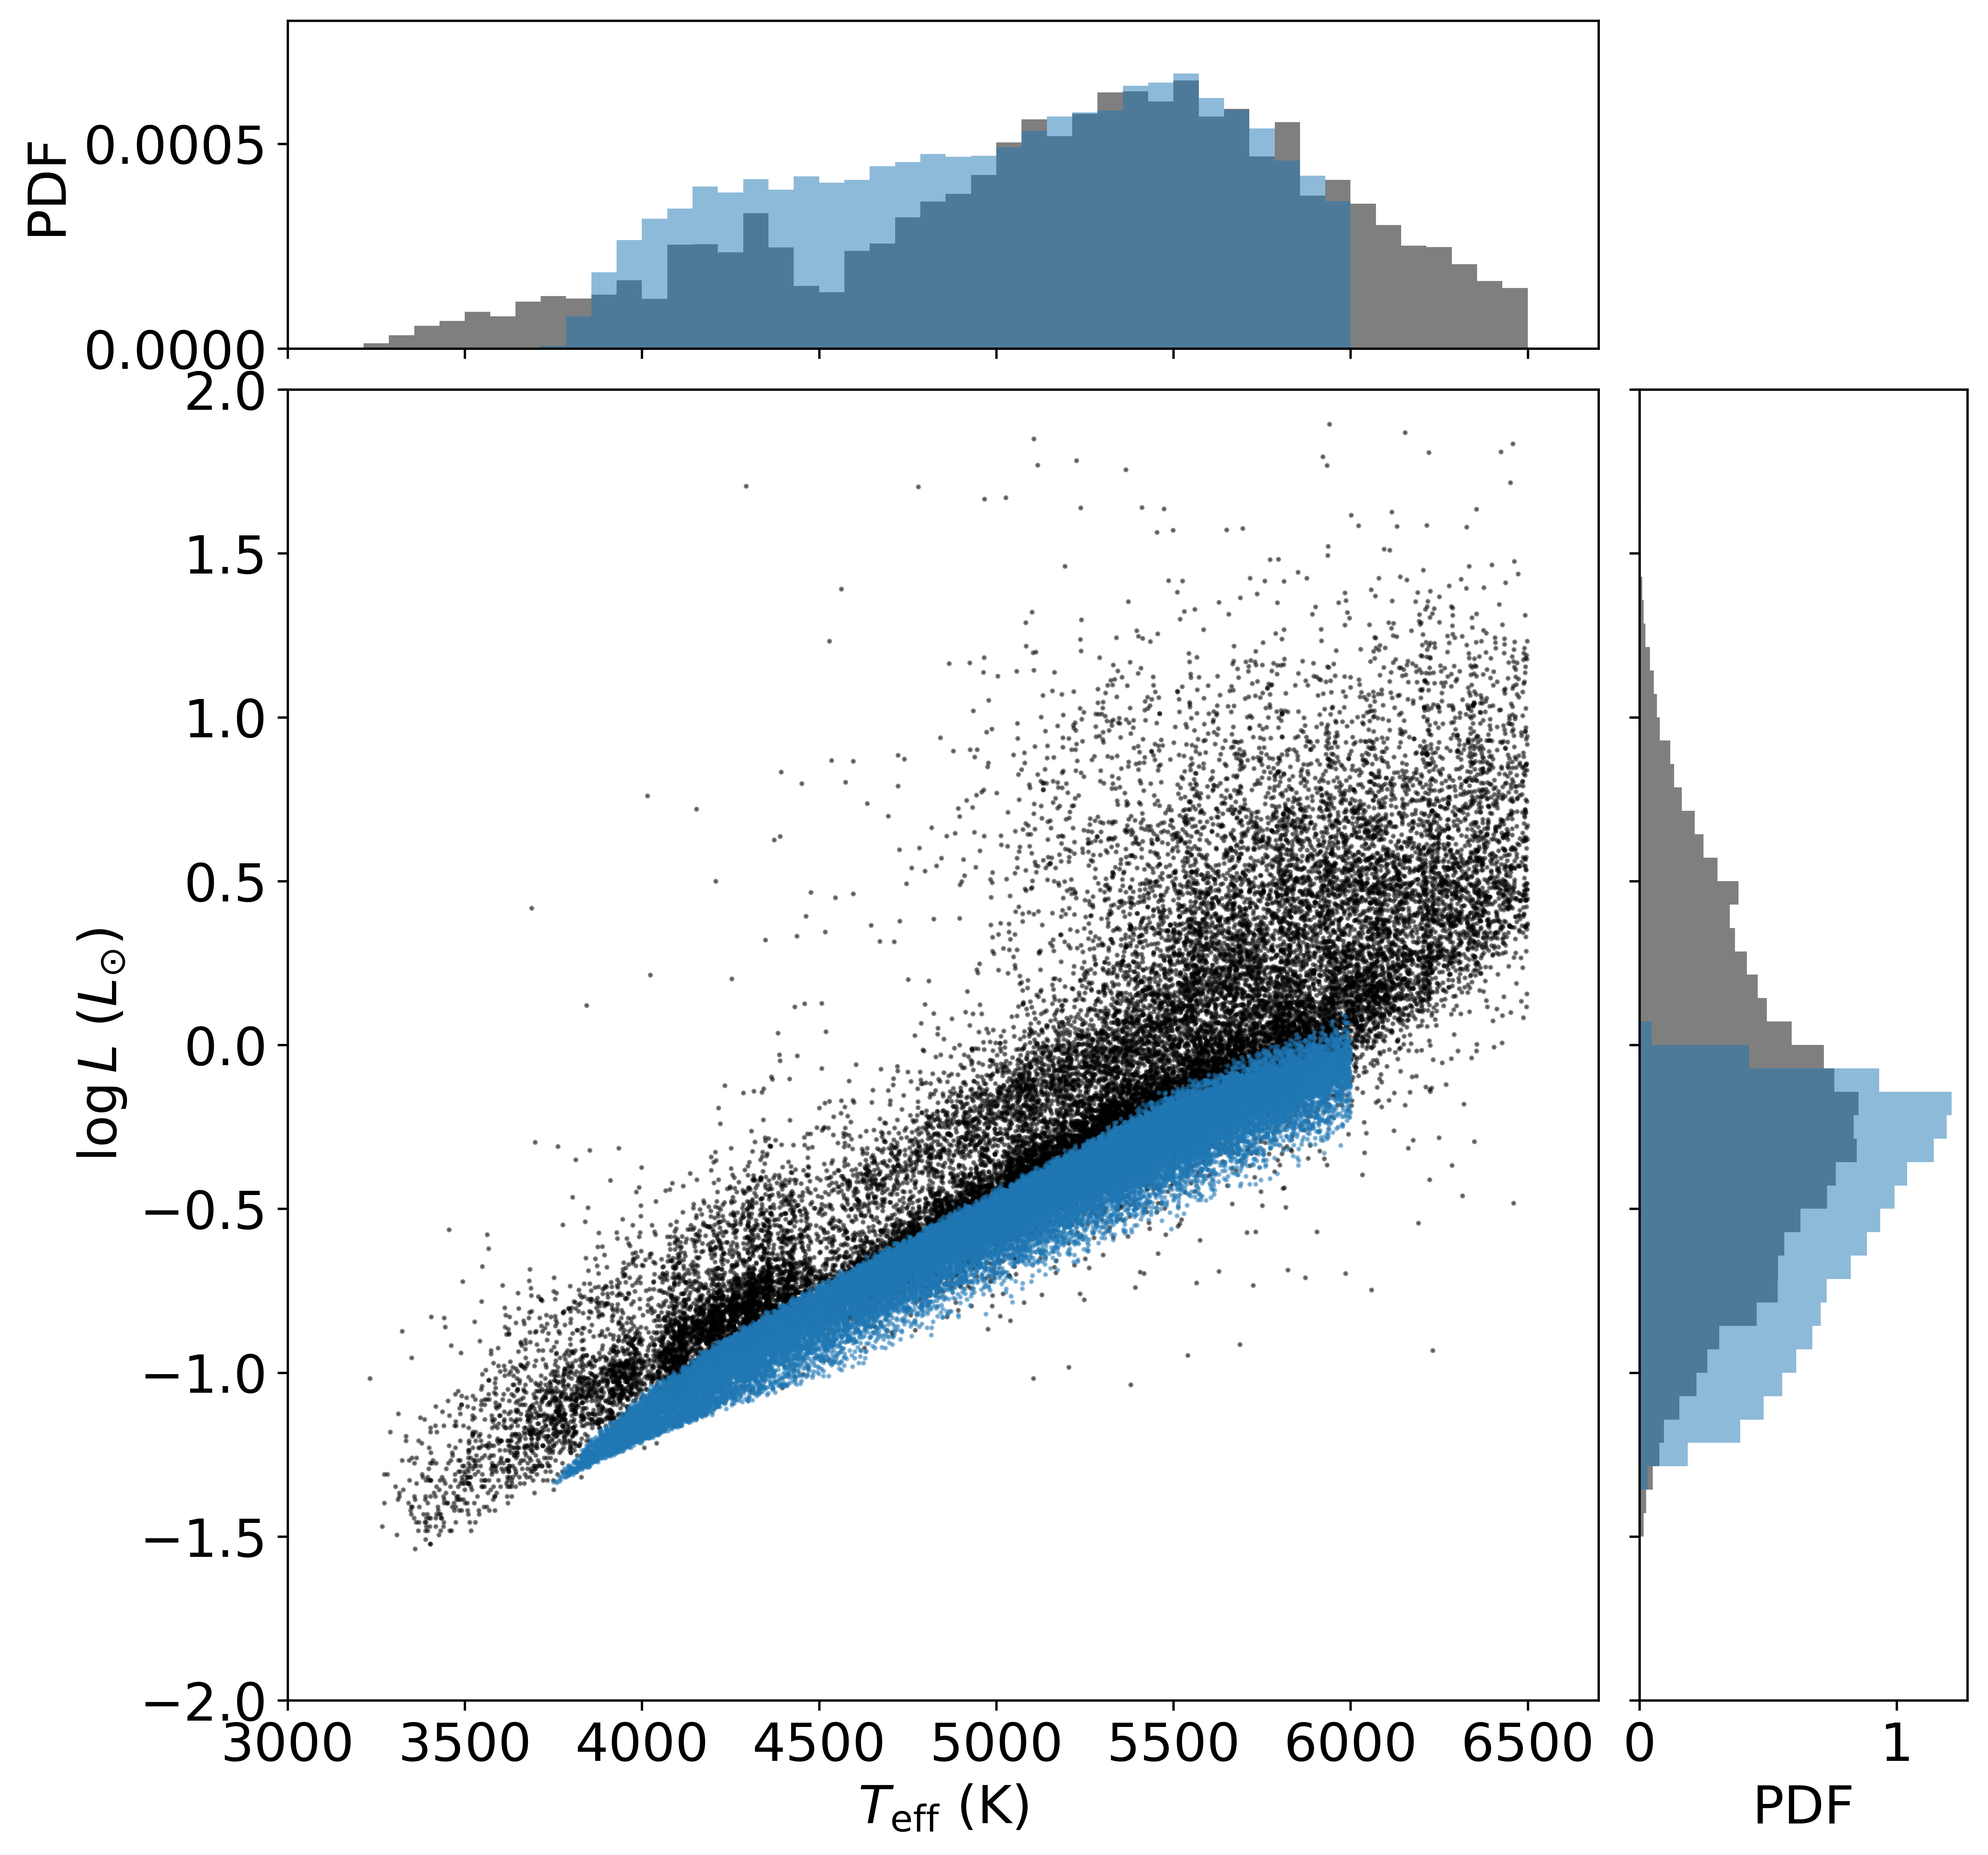
\includegraphics[width=\textwidth]{Figures/rot_gap_figures/compar_dist.png}
 \caption[A comparison between the effective temperature and luminosity distributions of the \citet{mcquillan_rotation_2014} and synthetic sample adopted in this work. ]{A scatter plot of effective temperature and luminosity distributions of the \citet{mcquillan_rotation_2014} (black) and synthetic sample (blue) adopted in this work. On the left and above, we also show the probability density distributions of the luminosity and effective temperature, respectively. The distributions generally agree, suggesting that a direct comparison between the distributions is sound.}
 \label{fig:compar_teff_logl}
\end{figure}

The Sun is believed to be currently transitioning from equator-fast to anti-equator-fast differential rotation.
As a result of this transition, the average observed rotation period will decrease suddenly.
We believe this may a feature of the measurement of the observed rotation period biased differential rotation.
In this work, we have identified the over-density of stars with solar $R_o$ and the shape of the upper left edge of the rotation period distribution.
While the observed \kepler{} rotation periods do contain a high density of stars near this location (the long-period pileup \citep{van_saders_forward_2019} ), we are hesitant to suggest whether this feature is the result of this transition or from the selection function of \kepler{} observations being biased towards higher mass, brighter, stars.
This over-density is also reflected in the equatorial rotation periods of our synthetic sample.
However, given that the observed rotation periods used to tune the generative model of our synthetic samples ``equatorial" rotation periods of high-mass stars may already be biased measurements, disentangling their relative effects is difficult.
Further, given the small number of nearby, old ($\geq$ 3 Gyr) clusters in the \kepler{} field and the evolution of rotational spin-down with variations to the latitudinal differential rotation, we believe that the cluster-tuned isochrones used in this work to determine the rotation periods of stars are less reliable for these stars.

The effects of differential rotation may already bias the adopted equatorial rotation periods in this work.
The \citet{spada_competing_2020} model can qualitatively reproduce the over-abundance of stars on the slow branch below the intermediate period gap through the introduction of mass-dependent core-envelope coupling.
However, it overestimates low-mass rotation periods for stars older than approximately a gigayear.
This limited the range of masses in our synthetic sample.
The effect of differential rotation on low-mass stars ($< \ 4000 K$), where the rotational period gap is most apparent, using a physically motivated synthetic sample of rotation periods was not possible.

In order to make these comparisons, we require a way of generating accurate equatorial rotation periods for low-mass stars.
We propose a follow-up work retuning the rotational isochrone model with the new information that the Ruphrecht 147 \citep{curtis_when_2020} and NGC6819 \citep{meibom_kepler_2011} cluster period distributions provide.
A model comparison could then be made to determine whether a model that does or does not include the effects of differential rotation on the observed rotation period better fits the observed rotational period distributions.
It is also worth noting that the parameters of their model may  be significantly degenerate with the effects of latitudinal differential rotation.
Without this work, we can only speculate.
 
A currently unaccounted feature of the intermediate period gap by our model is the decreased \rper{} of stars within the gap relative to the surrounding rotation periods.
We propose a mechanism to explain this feature.
The fractional spot coverage of young, fast rotators ($R_o \ < \ 0.2$) is saturated.
Above this regime, the fractional spot coverage drops rapidly (See Figure 7. in \citet{cao_starspots_2022}).
Latitudinal shear is, however, anticipated to serve as a catalyst for large-scale strong magnetic fields.
Further, latitudinal shear leads to differential twisting of the poloidal field lines, resulting in a bunching of field lines that result in active regions on the surfaces of stars \citep[see, e.g.,][]{berdyugina_starspots_2005, miesch_large-scale_2005, magnetism_brun_2017}
As latitudinal shear grows, we therefore speculate that the fractional spot coverage of stars could, in-turn, increase, leading to the observed increase in \rper{} above the gap.
We intend to investigate this testable hypothesis by measuring the fractional spot coverage of stars above the gap.

Further work to confirm the mechanism is required with more rigorous methods.
We propose the following investigations:
\begin{itemize}
	\item Observations of the differential rotation of nearby stars with Doppler imaging above and below the rotation period gap to search for evidence of variance to latitudinal differential rotation.
	\item Use of more rigorous models of the latitudinal expression of stellar spots and their effect on the observed rotation period of stars. Such an analysis could first be completed with non-uniform distributions of stellar spots on the surface of stars from magnetohydrodynamic simulations of rotating stars using a similar analysis to that performed in this work. We also propose a hare and hound investigation where lightcurves of a synthetic sample of stars with model-motivated stellar spot distributions and observationally motivated differential rotation profiles are then treated as data to determine whether the rotation period gap is recovered using methods of rotation period measurement.
	\item Finally, we propose further modelling work to determine the evolution of surface differential rotation of fully convective stars. If surface differential rotation is suppressed or otherwise peculiar from partially convective stars, then this mechanism can fully explain the observations of \citet{lu_bridging_2022}.
\end{itemize}

\section{Conclusions}
\label{sec:conclusione}

In this work, we have qualitatively shown that the transition from latitudinally-flat to equator-fast differential rotation can introduce a dearth of observations in a rotation period distribution.
The transition from latitudinally-flat to significant equator-fast differential rotation occurs precisely at $R_o \ = \ 0.45$ coincident with the intermediate period gap.
This suggests that the cause of the intermediate period gap is this transition.
We argue that the growth in latitudinal shear explains several features of the intermediate period gap, including the high density of stars above and below the gap and the decrease in photometric variability of stars within the gap.
The scale of the introduced dearth depends on highly uncertain parameters that may be degenerate: the latitudinal distribution of stellar spots and the relationship between $R_o$ and latitudinal shear, suggesting further explorations of the parameter space are required.
These results provide a novel explanation for the intermediate period gap without the requirement of new physics and underscores the need for further research into the impact of latitudinal differential rotation on observations of surface rotation of stars across the main-sequence. 
%
\newcommand{\todo}[1]{\textcolor{red}{#1}}

\chapter{Summary, Conclusions and Future Work}
\label{chap:conc}

\section{Summary}

Rotation is an often overlooked area of stellar astrophysics and astronomy due to its complexity in both modelling and observation.
That being said, over the previous decades, our understanding of the evolution of rotation and its impact on stellar evolution has grown dramatically.
With every observation of rotation that we make we are learning that our simple implementations and parameterisations in stellar evolution codes do not necessarily account for a number of misunderstood mechanisms underlying the evolution of rotating stars.
We are also learning that rotation can have impacts on the observations that we are able to make of stars.
This is the direct result of the growth of the data boom that we find ourselves in due to the sheer number of stars we have precisely photometrically observed over long-period baselines through missions such as \kepler, \ktoo and \tess.

Indeed, this thesis does not provide an exhaustive list of every single effect that rotation has on stellar evolution, nor every gap in our knowledge of its effects.
In this work, we have attempted to provide novel ways to improve our understanding of rotation, without the requirement of more data.
The title of this thesis was deliberately chosen as "Problems in low-mass stellar rotation" - because, while we do work to provide methods that may lead to conclusions about the effects that rotation has on stellar evolution, these are not closed problems.
We define a problem here as something that requires a resolution.

\section{Conclusions}

This thesis outlines three problems in low-mass stellar rotation and our attempts to address them through novel methods.
In Chapter \ref{chap:subgiant_ast} we first investigated the subgiant angular momentum transport problem.
This is the disparity between the observations of the core and surface rotation rates of subgiants and expected core and surface rotation rates from rotating models of stellar evolution.
Those observed core-to-surface rotation rate ratio of low-luminosity subgiants suggest angular momentum transport one to two orders of magnitude greater than the angular momentum transport currently implemented in rotating stellar evolution codes.
Stronger constraints to the internal rotation profile shapes of those low-luminosity subgiants would illuminate the excess angular momentum transport mechanism at play.
We have shown in this thesis that, through the application of distinct measurements of stellar rotation - specifically here asteroseismology and periodic photometric variability due to stellar spots - to more precisely constrain the internal rotation profile of low-luminosity subgiants.
While we have only applied this method to a single star, KIC 12508433, we believe the method is easily adopted in other studies to better constrain those internal rotation profiles better than either of those measurements of stellar rotation can individually - without the requirement of more data.

In Chapter \ref{chap:stellar_spots} we investigate the effect that stellar rotation can have on accurate and precise measurements of atmospheric metallicity and chemical abundances.
Accurate measurement of stellar metallicity can be an integral part of our understanding of the universe - from the understanding of the origin of elements in the universe to galactic archeology, to accurate aging of open clusters.
Astrophysicists rely on accurate measurements of atmospheric metallicity to constrain their models of stellar evolution and astronomers investigate the predictions made by those models.
This is a cyclic process where if astronomers do not adopt accurate models of the stellar atmosphere, inaccuracy compounds.
We created a sample of synthetic spotted stellar spectra with physically motivated stellar parameters to investigate the effect that adopting a non-spotted model of the stellar atmosphere has on the accuracy of recovered stellar parameters.
We found that even when adopting a naive model of the effect of stellar spots, through a two-temperature model of the stellar atmosphere, stellar spots introduce on average a 0.03 dex scatter to the measured metallicity of main-sequence stars.
This effect is non-negligible. 
A spotted model of the stellar atmosphere should be adopted, or the effect that this level of imprecision can have on our inferences of astrophysics should be considered, especially where precise inference of stellar metallicity is required.

Finally, in Chapter \ref{chap:period_gap} this thesis investigates the intermediate period gap.
The intermediate period gap is a currently unexplained phenomenon manifesting as a dearth of observations of particular stellar surface rotation periods from photometric variability due to stellar spots.
The two leading theoretical explanations for the rotational period gap are that the gap represents a minima of observability of rotational periods through a sudden decrease in photometric variability or that the gap represents a region of extreme angular momentum loss that causes stars to quickly physically "jump" the gap leading to a decreased number of stars with observed rotation periods.
If either of these hypotheses are the cause of the intermediate period gap then they have wider implications for our understanding of the evolution of magnetic activity or the angular momentum evolution of stars.
We first investigate these hypotheses through measurements of their magnetic activity through the chemical magnetic activity indicator $\log R^{+}_{\rm{HK}}$.
The decrease in photometric variability of stars toward the gap is possibly coincident with a decrease in $\log R^{+}_{\rm{HK}}$.
We argue that this suggests that the cause of the decrease in photometric variability and $\log R^{+}_{\rm{HK}}$ are one and the same.
If the decrease in photometric variability is the cause of the intermediate period gap, then the decrease in photometric variability should be reflected in a decrease to $\log R^{+}_{\rm{HK}}$.
We do not find evidence of an ultra-low magnetic activity subsample of stars in the \kepler-LAMOST crossmatch of stars without detected rotation periods, nor evidence of increased magnetic activity of stars above the gap, that would be indicative of extreme magnetic braking.
Furthermore, we show that the number of stars without detected rotation periods in the \kepler sample would need to make up a majority of the stars required to fill the rotation period gap.
In conjunction, these results suggest that the cause of the intermediate period gap is not a decrease in the detectability of the rotation of stars.
As a result of this conclusion, we propose another cause for the intermediate period gap: the onset of equator-fast latitudinal differential rotation at $R_o \approx 0.5$ and the variability of the distribution of stellar spot (latitudinally) on the surfaces of stars.
We show that, under the assumption that the observed rotational period of stars is the average rotation rate relative to the distribution of stellar spots on the surface of a star, and after adopting observationally and model-based relations between latitudinal differential rotation and stellar spot distributions on the surface of stars relative to equatorial rotation rate, the onset of latitudinal differential rotation results in a dearth of observations of stars precisely at the intermediate period gap.
While this result requires more thorough investigations into the effect of latitudinal differential rotation on the stellar light curve and therefore observed rotational period, this is a novel proposal that we argue explains all of the observational counterparts \footnote{or lack thereof in terms of the implied peculiarity} to the intermediate period gap without the requirement of new, and complex, physics.

\section{Future Work}

\subsection{Applications of our work}

In this work, we have presented representative studies that provide methods for improving our understanding of rotation in stars.
All of these works have further applications for the wider rotational astronomic community.

The application of a surface rotation prior to inference of the internal rotation profiles of low-luminosity subgiants is a novel way to further constrain the internal rotation profiles of stars without the requirement of more data.
Without this method, see e.g. \citet{albhorn} who suggest precise measurement of up to $\ell = 10$ mode rotational splittings are required for inference of the internal rotation profile of post-main-sequence stars using only the rotational splittings, inference of the internal rotation profile of stars will require extremely long baseline observations of a number of subgiants.
While plans are being made for longer-baseline asteroseismic missions \citep{haydn, plato, roman} the length of the missions required for such investigations (on the order of 10s of years) appear unfeasible - given the recent track record of the length of observational missions.
We, therefore, propose that this method be applied to our observations of post-main-sequence stars with measured rotational splittings.
As we discuss in the conclusion of Chapter \ref{chap:subgiant_ast}, this method can be applied to any star with observed rotational splittings and a measurement of the surface rotation rate.
This can either come in the form of surface rotational period measurements from the active regions of stars, as was adopted in that work and is a by-product of time series-based photometric observation missions, or through spectroscopic $v \sin{i}$.
The inclination angle and stellar radius, effects that usually plague the constraints to our measurements of stars are independently constrained through asteroseismic investigations of the star, making it possible to strongly constrain the surface rotation rates of stars in this way.
A good place to start in this respect is with the $\sim$30 subgiant stars for which rotational splittings have been observed.
The combination of the constraints to the internal rotation profiles of low-luminosity subgiants, in a population inference sense, may constrain the angular momentum transport mechanism underlying the post-main sequence angular momentum transport problem.

In regard to measuring the effect that stellar spots have on the measurement of the atmospheric metallicity of stars, there are a number of applications and extensions to our work that could be adopted.
The spectroscopic nature of active regions is a field in its infancy.
More modelling work is required to understand how the fundamental parameters of stars other than the Sun govern their magnetic fields and the properties of stellar spots.
Stellar spots likely have more complex contributions to spectra than the 2-temperature model we have adopted in that work.
Further, the effect of magnetic fields, the properties of stellar spots and the effect that they have on the stellar spectra are unknown.
For some stars, Doppler imaging is able to indirectly determine the spot contribution to stellar flux.
Investigations into the variance between spotted and unspotted stars, even through observations of the Sun, are required to more accurately parameterise the effect of stellar spots on stellar spectra.

For example, in this work we have only considered the effect that the cooler "spot" regions have on the inference of stellar parameters.
Indeed, as well as the cool regions, magnetically active regions can also be brighter, or hotter, than the ambient temperature of a star in the form of faculae.
The relative effect of faculae is, comparatively, unknown.
Algebraically, in the model we adopt, a star with a large fractional coverage of cool spots is the same as a star with a small fractional coverage of hot faculae.
This suggests that whether you adopt spots or faculae, scatter to inferred stellar parameters will be introduced.

To speculate: the contribution of spots and faculae could be disentangled from the stellar spectra using the method we adopt in this paper.
The cancellation of the contribution to the stellar flux from spots by faculae, and vice versa, is a proposed mechanism underlying the intermediate period gap that we are currently unable to investigate.
However, with a 3-temperature stellar spectra model of the stellar atmosphere, we could determine whether this is indeed the case.
We propose an investigation into the feasibility of using the reduced goodness of fit between a single and 3-temperature contribution stellar spectra of the same effective temperature of stars using a single and 3-temperature contribution model of the stellar spectra.

While this method cannot be used to directly image the stellar spots on the surfaces of stars, it can be used to determine the fractional spot coverage and the relative effect that they may have on observed variations to the stellar flux.
An area of concern when using the transit method for observing exoplanets is the degeneracy between transits and stellar spot contributions.
This method could be used to determine the spot contribution to the stellar spectra of stars with suspected exoplanetary transits.
Exoplanet transits have no impact on the stellar spectra they simply reduce the observed flux, but as described in our work, spots do.
A lack of variation to the stellar spectra before and during suspected transits would indicate that the transit is indeed a transit.

Finally, in this work, we investigated the nature of the intermediate period gap that we conclude is created by the onset of latitudinal differential rotation and variances to the latitudinal probability density function of stellar spots.
Confirmation of this conclusion using observations is difficult.
Constraining the scale of latitudinal differential rotation of main-sequence stars appears improbable using current photometric methods \citep[See Section 4.3 of]{aigrain_testing_2015}.
Fourier transforms of spectroscopic line profiles and time series Doppler image maps of the active regions of stars offer a possible avenue to explore in this regard (See \ref{sec:intro_diff_rot_techniques}).
We know at what observed rotation periods stars are below and above the gap, so a good first step would be to determine the scale of differential rotation (and stellar spot distribution) of stars with similar masses and varying observed stellar rotation periods.
Observation of little latitudinal differential rotation below the gap, and differential rotation above the gap would provide clear evidence for this being the main mechanism at play.

Furthermore, more investigations into the evolution of magnetic activity in regard to rotation are required.
Only recently has the observation that magnetic activity, through the fractional spot coverage of stars, varies as a result of core-envelope recoupling been made.
While we believe that the cause of the decreased photometric variability of stars just below the rotational period gap is the result of core-envelope recoupling, we do not have a clear explanation for the increase in magnetic activity as stars evolve beyond the rotational period gap.
Further studies into the differential rotation, radially and latitudinally, are required to understand why and how this occurs.

\subsection{The future of asteroseismology and observation of stellar rotation through photometric modulation}

While the second \kepler{} mission ended five years ago, the data is still being investigated.
A number of stars, especially low-luminosity subgiants, from whom we can determine core and surface rotation rates, are yet to be asteroseismically investigated.
We have shown in this work that the internal rotation profile shape of these stars cannot be measured with current measurements of the rotational splittings.
Further, the feasibility of determining the internal rotation profile of these stars, without dedicated long-term photometric missions is low.
That being said, the data boom we are currently experiencing, in regard to photometric data, does not appear to be slowing.
The \TESS{} photometric mission has, at the time of writing, been collecting short cadence data for over 4 years.
High-resolution observations of stars have been made that will bring with them a new observing field of stars through which we will be able to measure surface rotation periods, as well as rotational splittings, especially within its continuous viewing zones.
With this data more and more stars have their surface rotation periods \citep{claytor__2023} and rotational splittings determined.
With the accurate measurement of those quantities, and application of our proposed method to place stronger constraints on the internal rotation profile of these stars with a surface rotation rate constraint, a population inference approach appears as the approach to answering the post-main sequence angular momentum transport problem.

Proposals have been made for targeted high-precision asteroseismically-focussed missions: PLAnetary Transits and Oscillations of stars (PLATO) \citep{}, the High-precision AsteroseismologY of DeNse stellar fields (HAYDN) mission \citep{}.
With these missions, our understanding of the nature of the rotation of stars will grow.
Both from a larger sample of stars with more precise photometric observations and with longer baselines, which will result in more stars with a larger number of and more precise measurements of rotational splittings, as well as a larger sample of stars with photometrically measured surface rotation rates.

We will not speculate what the next problems in the low-mass stellar rotation will be, but with this level of data, we are certainly focussing on 2nd and 3rd-order effects of rotation which will no doubt improve our understanding of the evolution of rotation in stars and the effects that it has on the observations that we make.







%% ----------------------------------------------------------------
% Now begin the Appendices, including them as separate files
%
%\addtocontents{toc}{\vspace{2em}} % Add a gap in the Contents, for aesthetics
%
%\appendix % Cue to tell LaTeX that the following 'chapters' are Appendices
%
%% \newcommand\apogee{\project{APOGEE}}


\chapter{An investigation into the evidence against current explanations for the intermediate period gap}
\label{apndx:magnetic}

In this Appendix, we investigate the evidence for the two leading explanations for the intermediate period gap.
This work is intended to be treated as a companion and motivation for Chapter \ref{chap:period_gap} where we propose a novel explanation for the intermediate period gap through the onset of equator fast latitudinal differential rotation.
We separate the two for ease of readability.

\section{Introduction}

There are two leading explanations for the intermediate period gap.
They are, that the gap arises from a decrease in probability to observe rotation periods of stars precisely within the gap or that, through the onset of strong magnetic braking, stars suddenly ``jump" in surface rotation period, leading to dearth of observations\footnote{as to not repeat ourselves we direct you to our introduction of these mechanisms in Chapter \ref{chap:period_gap}}.
We propose here that the data does not support either of these explanations.
Before we can begin however it is worth discussing two concepts, the difference between the probability of observation, and the detectability of rotation period and the so-called magnetic activity indicators.

In this work we will use the terms probability of observation of rotation, and detectability of rotation period.
While they are related, they are different terms.
The detectability of rotation requires a relatively short cadence, on the time scale of days-weeks, observations with distinct variability in the light curve due to spots or faculae.
It depends on several factors on a star-to-star basis, including the inclination angle, wherein the magnetic activity cycle observations are made, where faculae and spots are distributed on the star's surface, and the lifetimes of these surface features relative to the star's rotation period. \citep{aigrain_hare_2015, reinhold_transition_2019, reinhold_where_2021}.
The probability of observation of rotation refers to a more stellar parameter-based average statistic under the comparison of the set of stars with and without detection rotation periods.
The detectability of rotation with fundamental stellar properties (temperature, metallicity, stellar age etc.) has been previously investigated.
Cool stars, especially cooler than 5200K, have a significantly higher probability of rotational period observation than hotter stars.
Cool stars both tend to have higher magnetic activity, and therefore more spots, and also have more significant brightness variations as a result of the same level of surface spot activity compared to hotter stars \citep{ mcquillan_rotation_2014, santos_surface_2021, zhang_magnetic_2020}
A relation with metallicity has also been investigated \citep{amard_evidence_2020,see_photometric_2021,claytor_tess_2023}.
Higher-metallicity ([Fe/H] $\gtrsim$ -0.1) stars \update{tend to have a higher rotation period detection rate} than lower-metallicity stars.
 \citet{avallone_rotation_2022, masuda_detectability_2022} separate the metallicity dependence from age and suggest that this effect arises from the fact that younger, more active stars are enriched by metals from Galactic chemical evolution rather than a result of the metallicity on the evolution of magnetic activity and probability of rotational observation.
Older stars tend to have a lower probability of observation. 
Their rotation periods are long and thus require a longer baseline of observations, and they tend to have weaker magnetic fields and thus express a smaller number of stellar spots.
Many stars cannot have their rotation periods measured purely from the inclination angle's effect on the rotation's detectability.
If a star is pole-on, even if a star expresses surface features close to the axis of rotation, no variance in the brightness of that star will be detected.
Increasing the sensitivity of telescopes, and methods of determining rotation periods, increase the number of stars that can have their rotation periods detected.
Still, this number is bounded by the subsample of stars that cannot have their rotation measured.
While the distribution of the inclination angle of stars is biased toward equator-on observations, a non-zero population of stars will never have their rotation periods detected through photometric variability.

\subsection*{Stellar magnetic activity indicators}
\label{sec:act_ind}

Stellar magnetism is a complex component of stellar evolution that is hard to predict and model.
Links between magnetism and mass, metallicity, age, convection, and rotation have been identified \citep{cao_starspots_2022}.
These links are, however, based upon observations of stars rather than theory.
The observation of rotational modulation in a light curve, and the observation of surface rotation from that modulation, requires cool spots and bright faculae created by concentrated magnetic fields near the surface of a star.
Stars with stronger magnetic fields tend to express larger spot coverage, thus having larger rotational photometric modulation and more readily observable rotation periods.

Stellar activity is the collective term used to describe different effects magnetic fields have on stars.
This name arises from the variability phenomena occurring from structured magnetic fields emerging from the convective envelope of stars.
For example, flares and large-scale photometric variability from stellar surface features (stellar spots or faculae).
The strength of the magnetic field can be directly or indirectly measured in several ways, and a star's photometric variance varies with the magnetic field's strength.
Here we will discuss three indicators of a star's magnetic field: the elemental magnetic activity through $\log R^{+}_{\rm{H,K}}$ and $S$, the photometric variability range (\rper) and the fractional spot coverage of a star ($f_{\rm{spot}}$).

One of the most frequently probed indicators of chromospheric activity, and thus magnetic field strength, in low-mass magnetically active stars is the non-thermal flux reversal in the cores of the Ca II H and K lines at 3968\,\AA\ and 3933\,\AA\, respectively.
Two measures of the chromospheric Ca II $H$ and $K$ line fluxes are generally adopted.
The first is through the classical $S$ index.
This is the flux ratio in the core of the Ca II $H$ and $K$ lines to close by continuous windows
\begin{equation}
S = \alpha \ \frac{H+K}{R+V},
\end{equation}
where $H$ and $K$ are the line fluxes measured in 1.09\,\AA\-wide triangular bandpasses while $R$ and $V$ are estimates of the continuum on either side of the lines measured in 20\,\AA\-wide spectral windows centred on 3901\AA and 4001\AA. 
$\alpha$ is a normalisation constant dependent on the telescope used to make the measurements, providing a link between samples.
The quantity $S$ is sensitive to the integrated emission over these windows and the photospheric radiation transmitted in the $H$ and $K$ passbands. 
$S$ is, therefore, evolutionary and metallicity dependent, which renders direct comparison of $S$ between different spectral type stars unsuitable.
The quantity $\log R^{+}_{\rm{H,K}}$, on the other hand, eliminates this contribution \citep[see, e.g. ][]{lorenzo_solar_2018} and is thus a more reliable measure of the chromospheric Ca II $H$ and $K$ flux.

Another indirect measure of the magnetic field's strength arises from the star's photometric variability.
Here we differentiate between the large-scale photometric variability of a star during a magnetic activity cycle, where the average stellar flux of a star increases and decreases on the timescale of years and the variability range of a star due to stellar spots on a rotational time scale.
The solar integrated Ca II index, $S$, correlates linearly with photospheric star-spot number.
 \citet{lorenzo_fine_2016, lorenzo_solar_2018} established a relationship between solar chromospheric activity and the number of spots on the surface for solar-like stars, suggesting that the two are interconnected. 
However, whether this correlation is strong enough to derive long-term chromospheric activity cycles similar to photometric cycles on magnetic activity timescales (years) is uncertain.
The consistently similar periods of the two relations suggest the two are interconnected, with the faculae or star spot dominance of the magnetic photometric cycles being derived from the expected relation between the two.
A star that expresses a larger number of stellar spots will have a more significant photometric variability as it rotates.

Photometric variability is generally measured through the quantity \rper{}.
\rper{} is defined as the median of the range between the 5th and 95th percentile of normalised flux in bins of the light-curve divided into sections of the length of the measured rotational period \citep{mcquillan_rotation_2014}.
Larger \rper{} stars are expected to have more easily detectable rotation periods because the larger the star's variability as it rotates, the more easily distinguishable this variability is from noise.

Finally, the most recent measure of stellar activity has arisen from the measurement of the fractional spot coverage of stars (See Chapter \ref{chap:stellar_spots} and \citet{cao_starspots_2022}).
They found that fitting \apogee spectra with two temperature components allows one to infer the surface fractional spot coverage and the temperature contrast of the spots to the ambient surroundings.
The fractional stellar spot coverage of a stars is expected to be tied to the photometric variability of those stars with larger photometric variability arising from a larger fractional spot coverage.

All of these measurements of magnetic activity have been shown to be related to each other and follow similar relations with the stellar Rossby number.
Magnetic activity indicators saturate below a $R_o<0.3$ \citep{cao_starspots_2022} (fast rotation) and decrease with a power law as $R_o$ increases.
This relation reflects the decreased probability of observing older slow-rotating stars in the \citet{mcquillan_rotation_2014} sample.
Variations in magnetic activity can therefore indicate variations to the expression of stellar spots and, thus, the observability of stellar rotation.

The magnetic activity also varies with the stellar magnetic cycle of a star, with some scatter to magnetic activity indicators being attributed to this.
Therefore, a single temporal measurement of magnetic activity must be treated with care.
Variations to the magnetic activity of stars, in a population-wide sense, should be found by the average magnetic activity of a subpopulation.
We adopt a population study approach to minimise this effect in this work.

This Appendix will be structured as follows.
In Section \ref{sec:minima_rper}, we introduce our method to determine where minima in photometric variability occur and reconfirm that the gap aligns with minima in the photometric variability range. 
Using this method, in Section \ref{sec:minima_rhk}, we show that this minima also aligns with minima in $\log R^{+}_{\rm{HK}}$.
Following this, in Section \ref{sec:low_activity_gap}, we then show that the sample of stars with undetected rotation does not contain a subsample of stars with magnetic activity low enough to fall below the rotation-detection threshold.
Then, in Section \ref{sec:no_gap_stars}, we argue that the number of stars required for the dearth of observations to no longer be considered a dearth requires a larger number of stars than the number of stars within the undetected sample.
In Sections \ref{sec:summary} and \ref{sec:conclusion}, we summarise and discuss the implications of our work on proposed mechanisms to explain the intermediate period gap.

\section{The gap aligns with a minima in photometric variability}
\label{sec:minima_rper}

The first mechanism we consider is that the rotation period gap reflects a decrease in photometric variability due to a variation in the magnetic field strength of stars near the gap.
We will begin with the 33,000 stars with rotation periods from \citet{mcquillan_rotation_2014}.
While this sample has been superseded by other missions in terms of sensitivity, the increase in sensitivity has \textit{not} increased the number of detected rotation periods of cooler stars, particularly where the gap is most apparent.
In terms of number of stars, it is still the state-of-the-art mission for precise measurement of the rotation periods of low-mass stars near the intermediate period gap.
All stars in this sample lay within the crossmatch with \gaia{} data release 3, which contains precise measurements of the $B_P - R_P$ colour, $G$-band magnitude and distance from parallax.
\update{We limit our sample to stars within the nearest 525pc, to avoid selection effects and inaccurate measurement of rotation periods of stars beyond this distance.
This reduces the sample to 8,594 stars.}
We made cuts in Gaia DR3 magnitudes and colours using $M_G$ $\geq$ 0 and $B_P - R_P \geq 0.8$ to target below the main-sequence turnoff and star's lower mass than the Kraft break \citep{kraft_studies_1967}.
This leaves us with a sample of 6,243 nearby stars with reliable surface rotation and colour measurements.
These measurements are shown in Figures \ref{fig:hr} and \ref{fig:prawn}, where we have plotted them as a colour-magnitude diagram and log rotation period against \gaia{} $B_P-R_P$ colour, what we will refer to as the rotational period distribution from in this work.
In Figure \ref{fig:prawn} we have also coloured the measurements by the $\log$ of \rper{}, which exhibits the decrease in photometric variability surrounding the gap.

\begin{figure}
\centering
  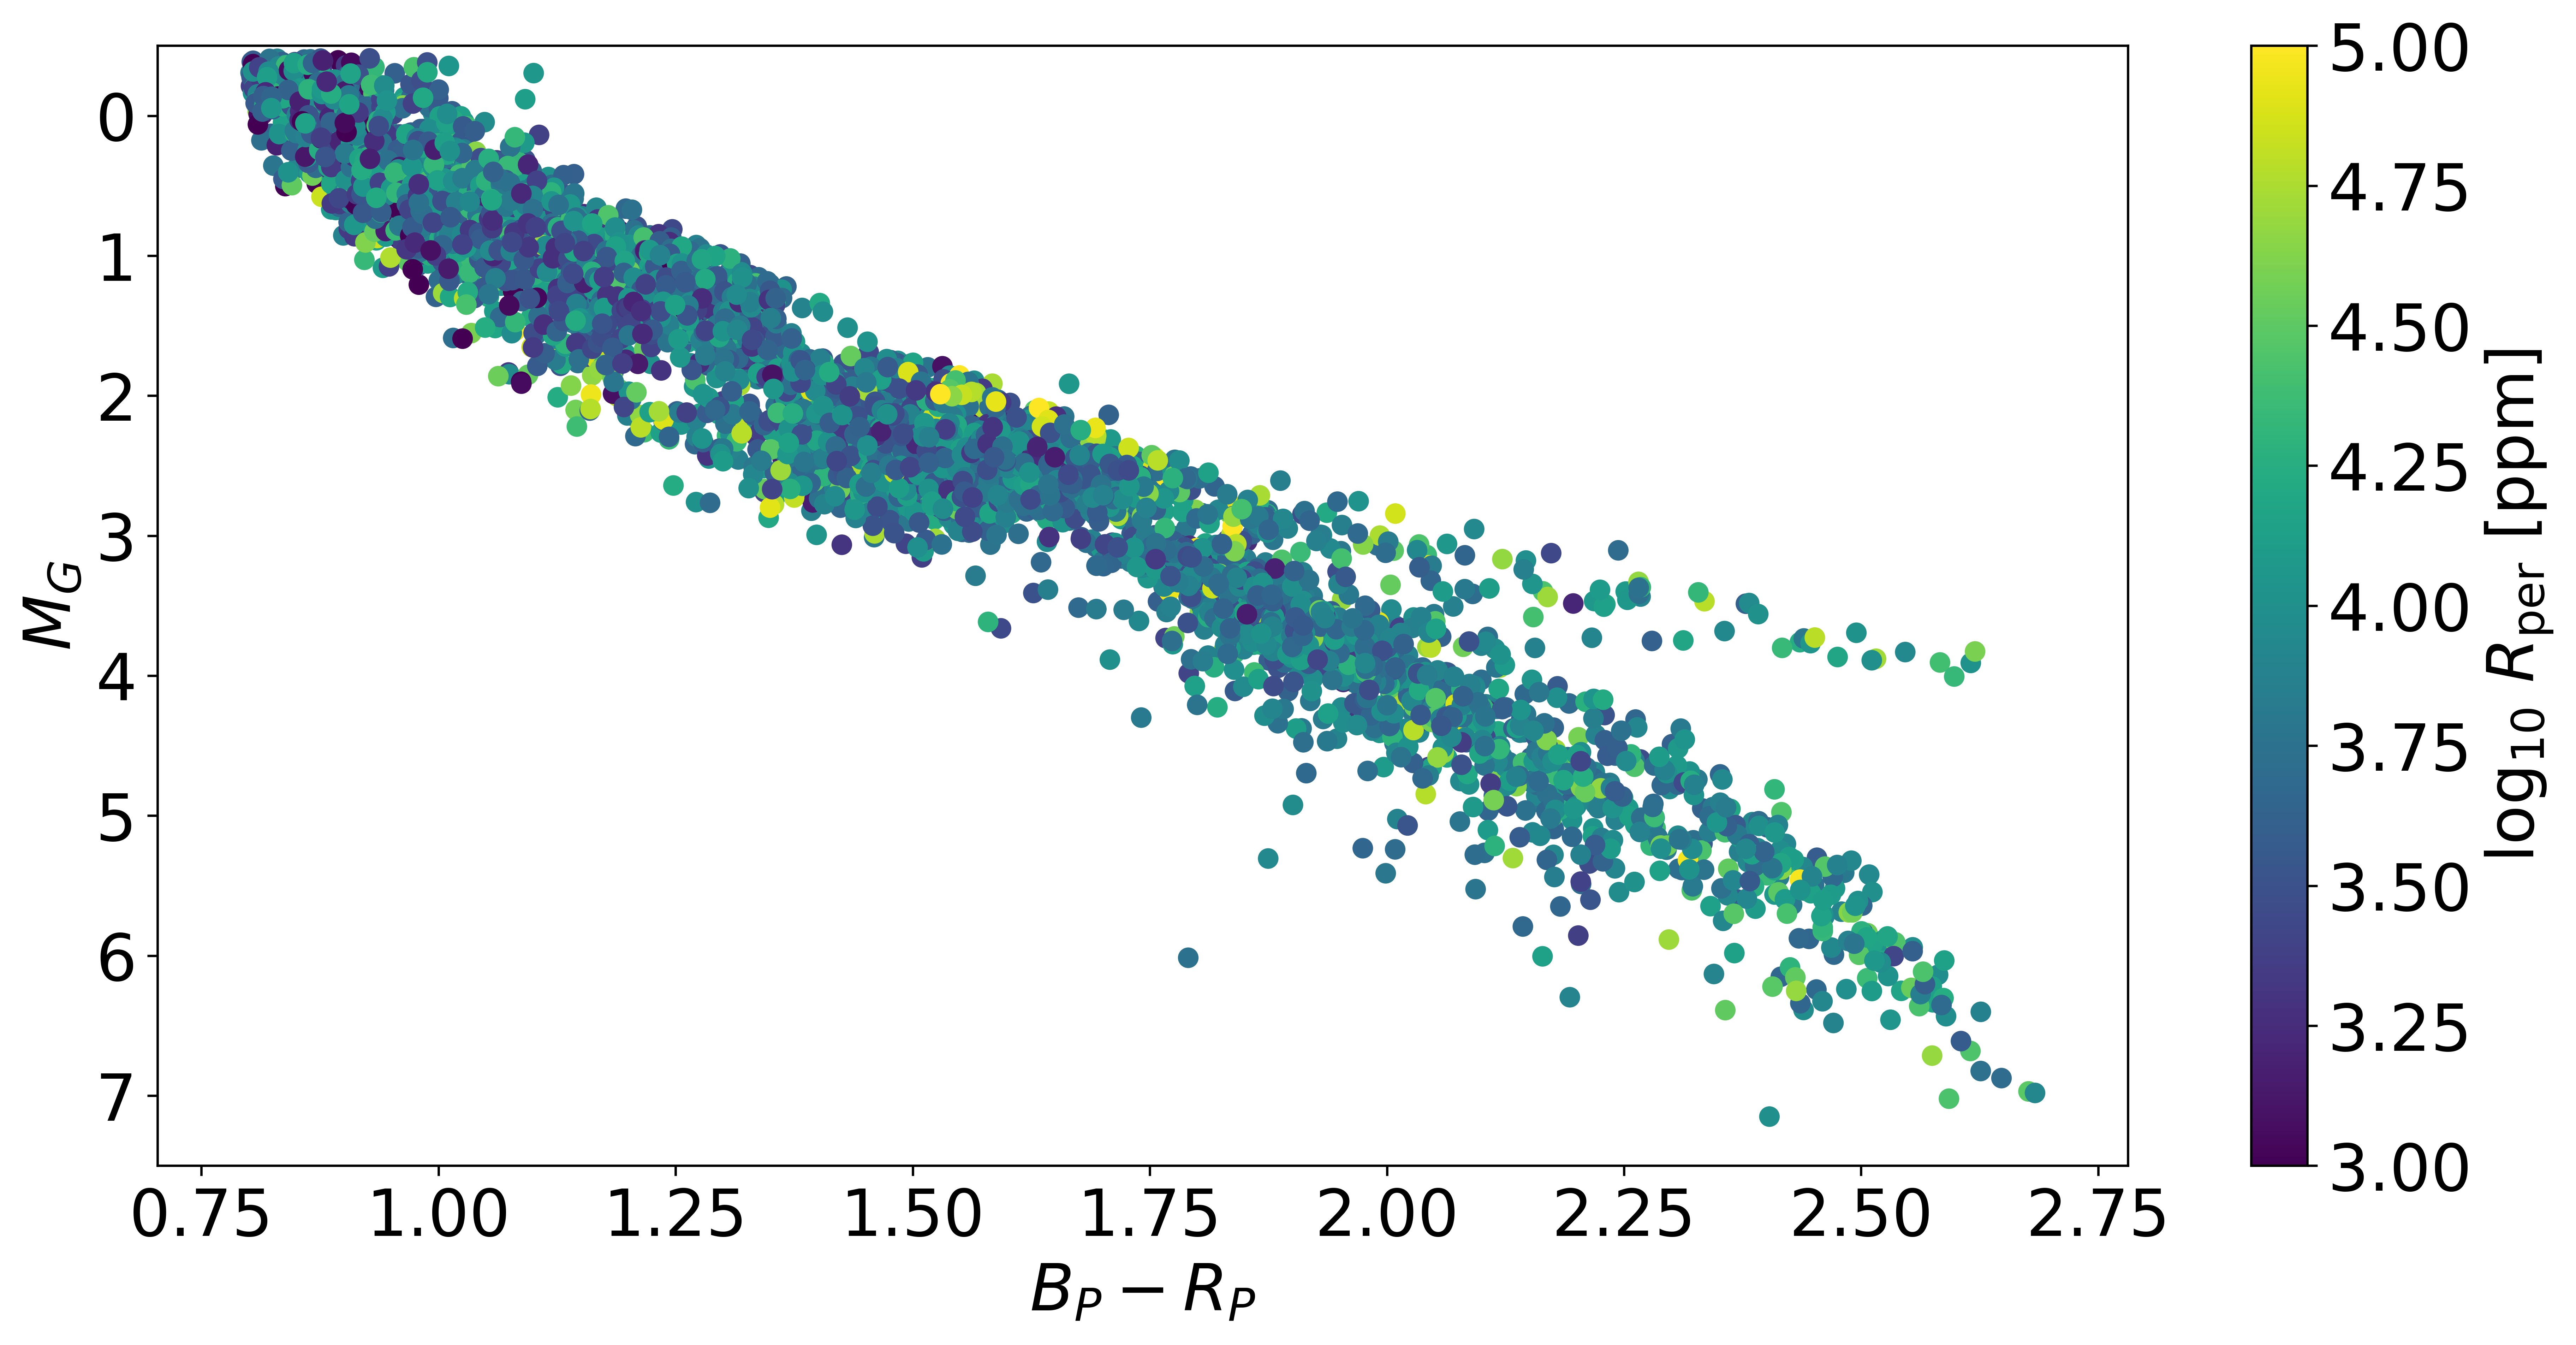
\includegraphics[width=\textwidth]{Figures/rot_gap_figures/HR.png}
  \caption[Colour-magnitude diagram of the closeby rotating main-sequence sample colours by photometric variability (\rper{}).]{
  Colour-magnitude diagram of the closeby rotating main-sequence sample colours by photometric variability (\rper{}).}
  \label{fig:hr}
\end{figure}

\begin{figure}
\centering
  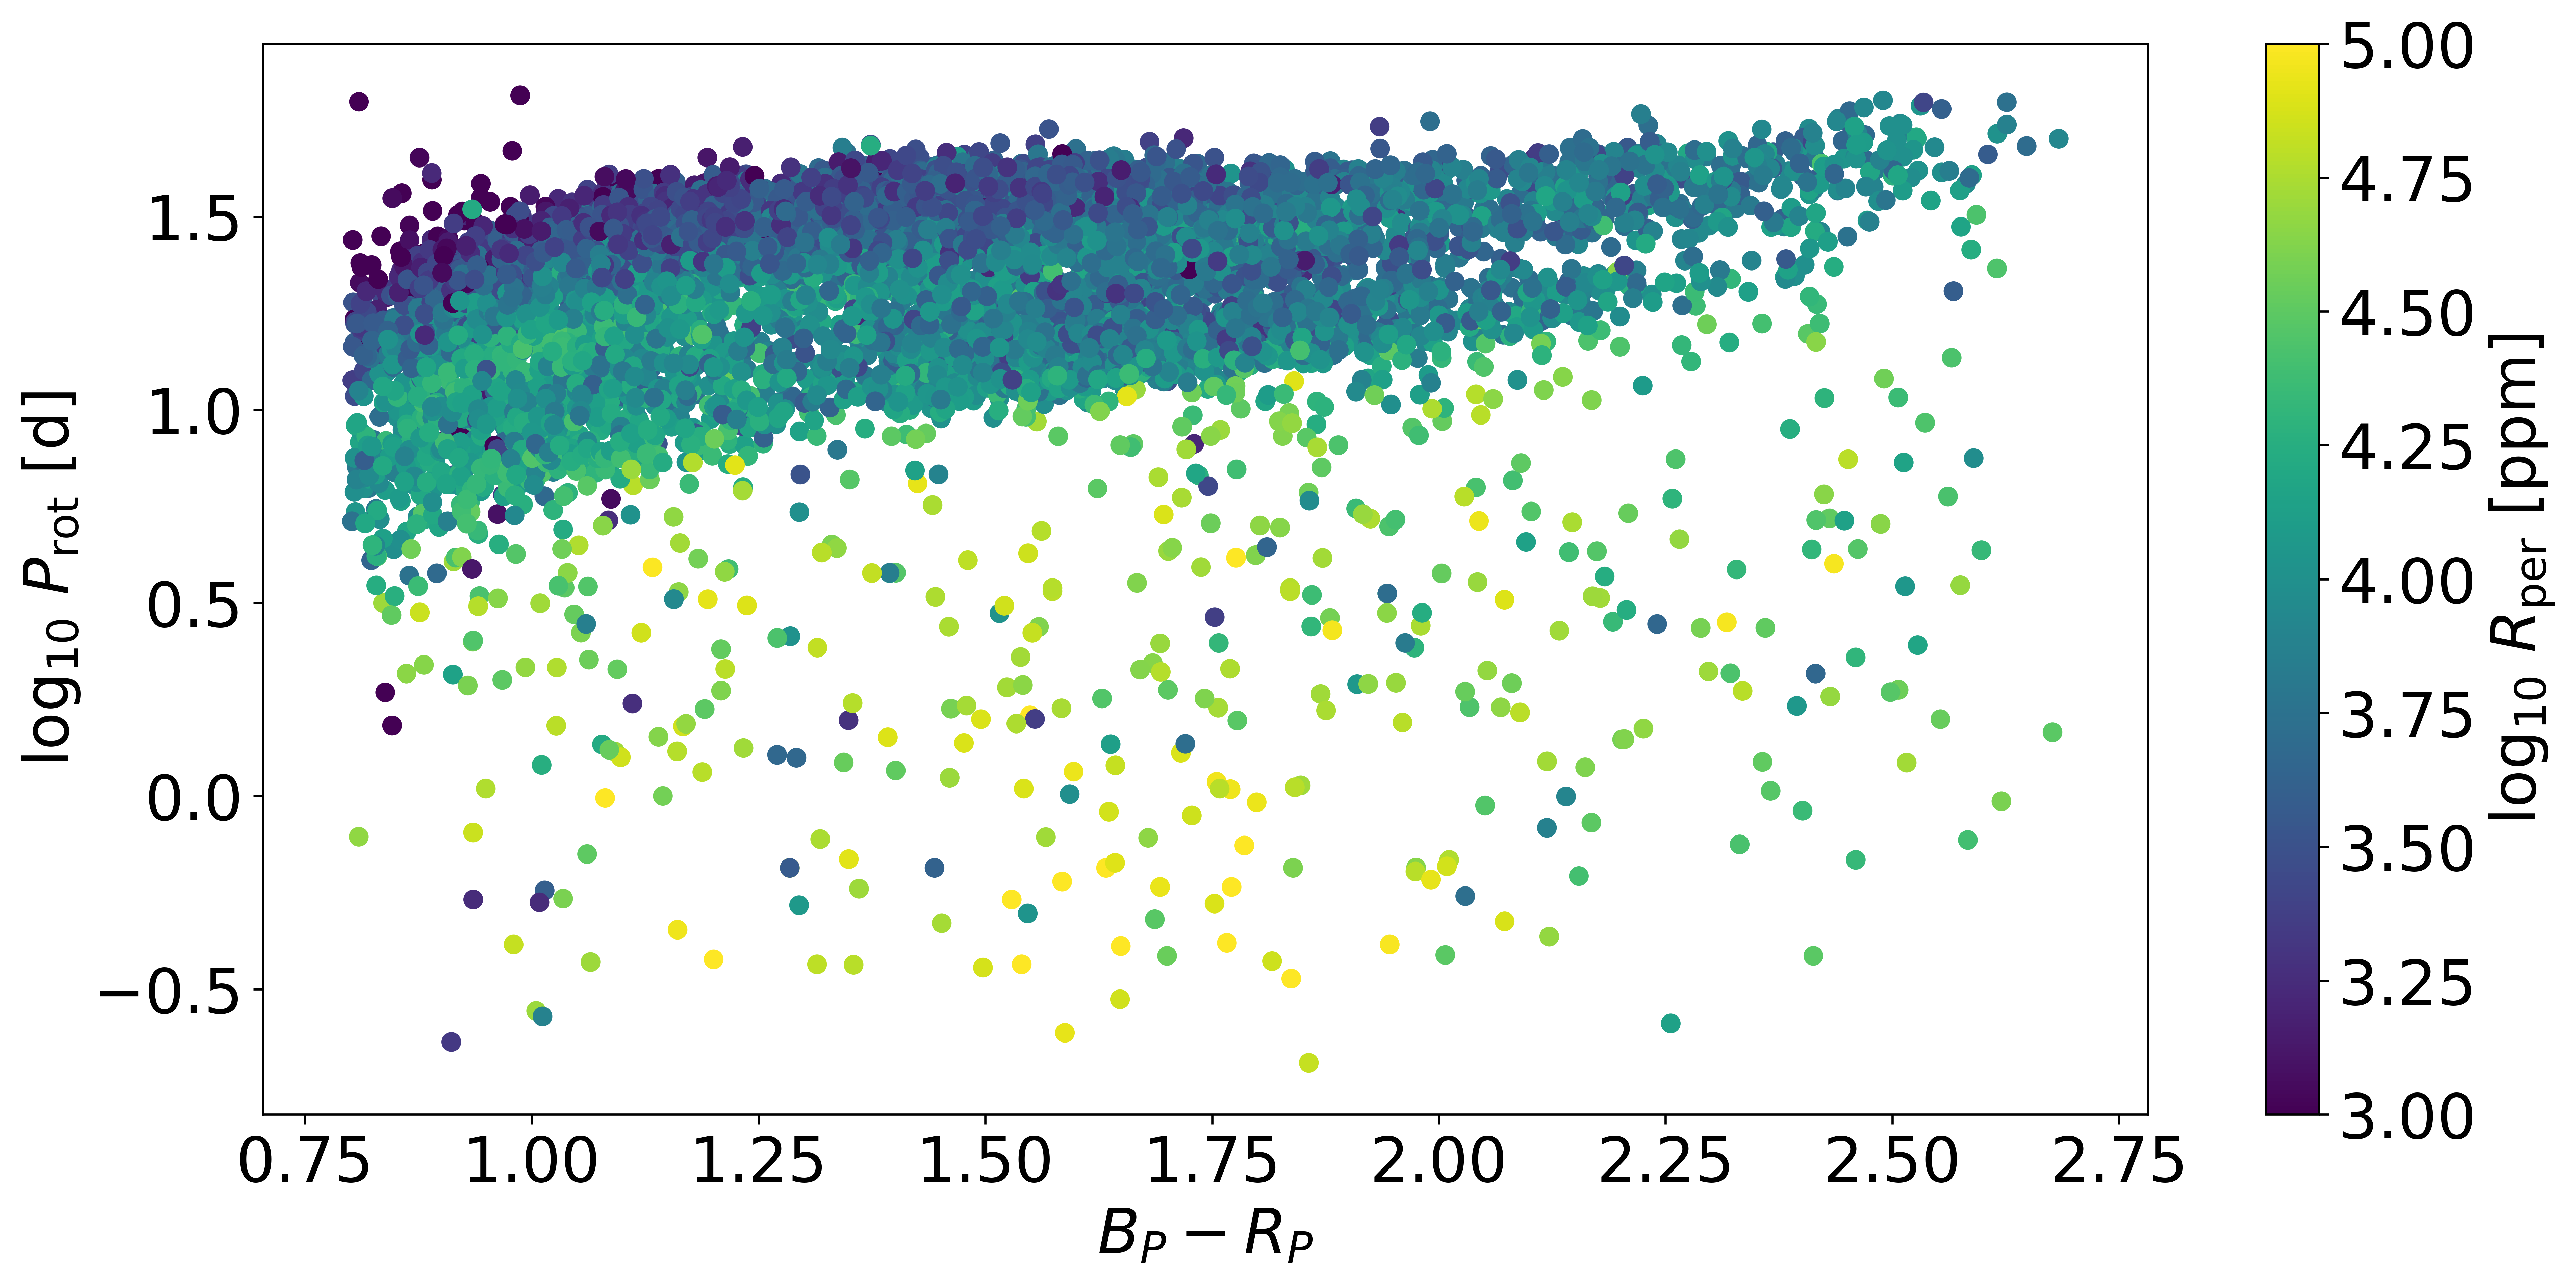
\includegraphics[width=\textwidth]{Figures/rot_gap_figures/rotational_dist.png}
  \caption[$\log_{10}$ of the rotation period against \GDRT\ $B_P-R_P$ colour of the closeby rotating main-sequence sample colours by photometric variability (\rper{}).]{
  $\log_{10}$ of the rotation period against \GDRT\ $B_P-R_P$ colour of the closeby rotating main-sequence sample colours by photometric variability (\rper{}). 
In this figure, we can see observe the decrease in the photometric variability of stars near the gap.}
  \label{fig:prawn}
\end{figure}

From this sample, we can describe the average evolution of photometric variability around the intermediate period gap.
We will first separate the subsample into bins of $B_P - R_P$ (colour) from 0.8-2.5 of size 0.17 (10 bins).
In each colour interval, we then split the data into the logarithm of rotational period intervals of width 0.07 dex between 0.4 and 1.8 dex, which correspond to 2.5 and 70 days, respectively.
We then compute the median and median absolute deviation of \rper{} in each colour and rotational period bin.
The median is used here to attempt to alleviate the effect of activity cycles on the variance of the magnetic activity, and the median absolute deviation establishes the scatter on the measured photometric variability: regions with large median absolute deviation should be treated as less reliable measurements.
We neglected the regions with few stars ($<$5).
This removes the spurious stars that have not ascended onto the lower prong of the intermediate period gap, which does not indicate large-scale trends in the data.
We reconfirm that \rper{} tends to increase with mass, decrease with the rotational period, and decrease towards the rotational period gap \citep{reinhold_stellar_2020, basri_double_2018, santos_surface_2021}.
Comparing Figures \ref{fig:prawn} and \ref{fig:binned_rper_full_sample}, we also confirm that the gap aligns itself with a minima in \rper{}.

\begin{figure}
\centering
  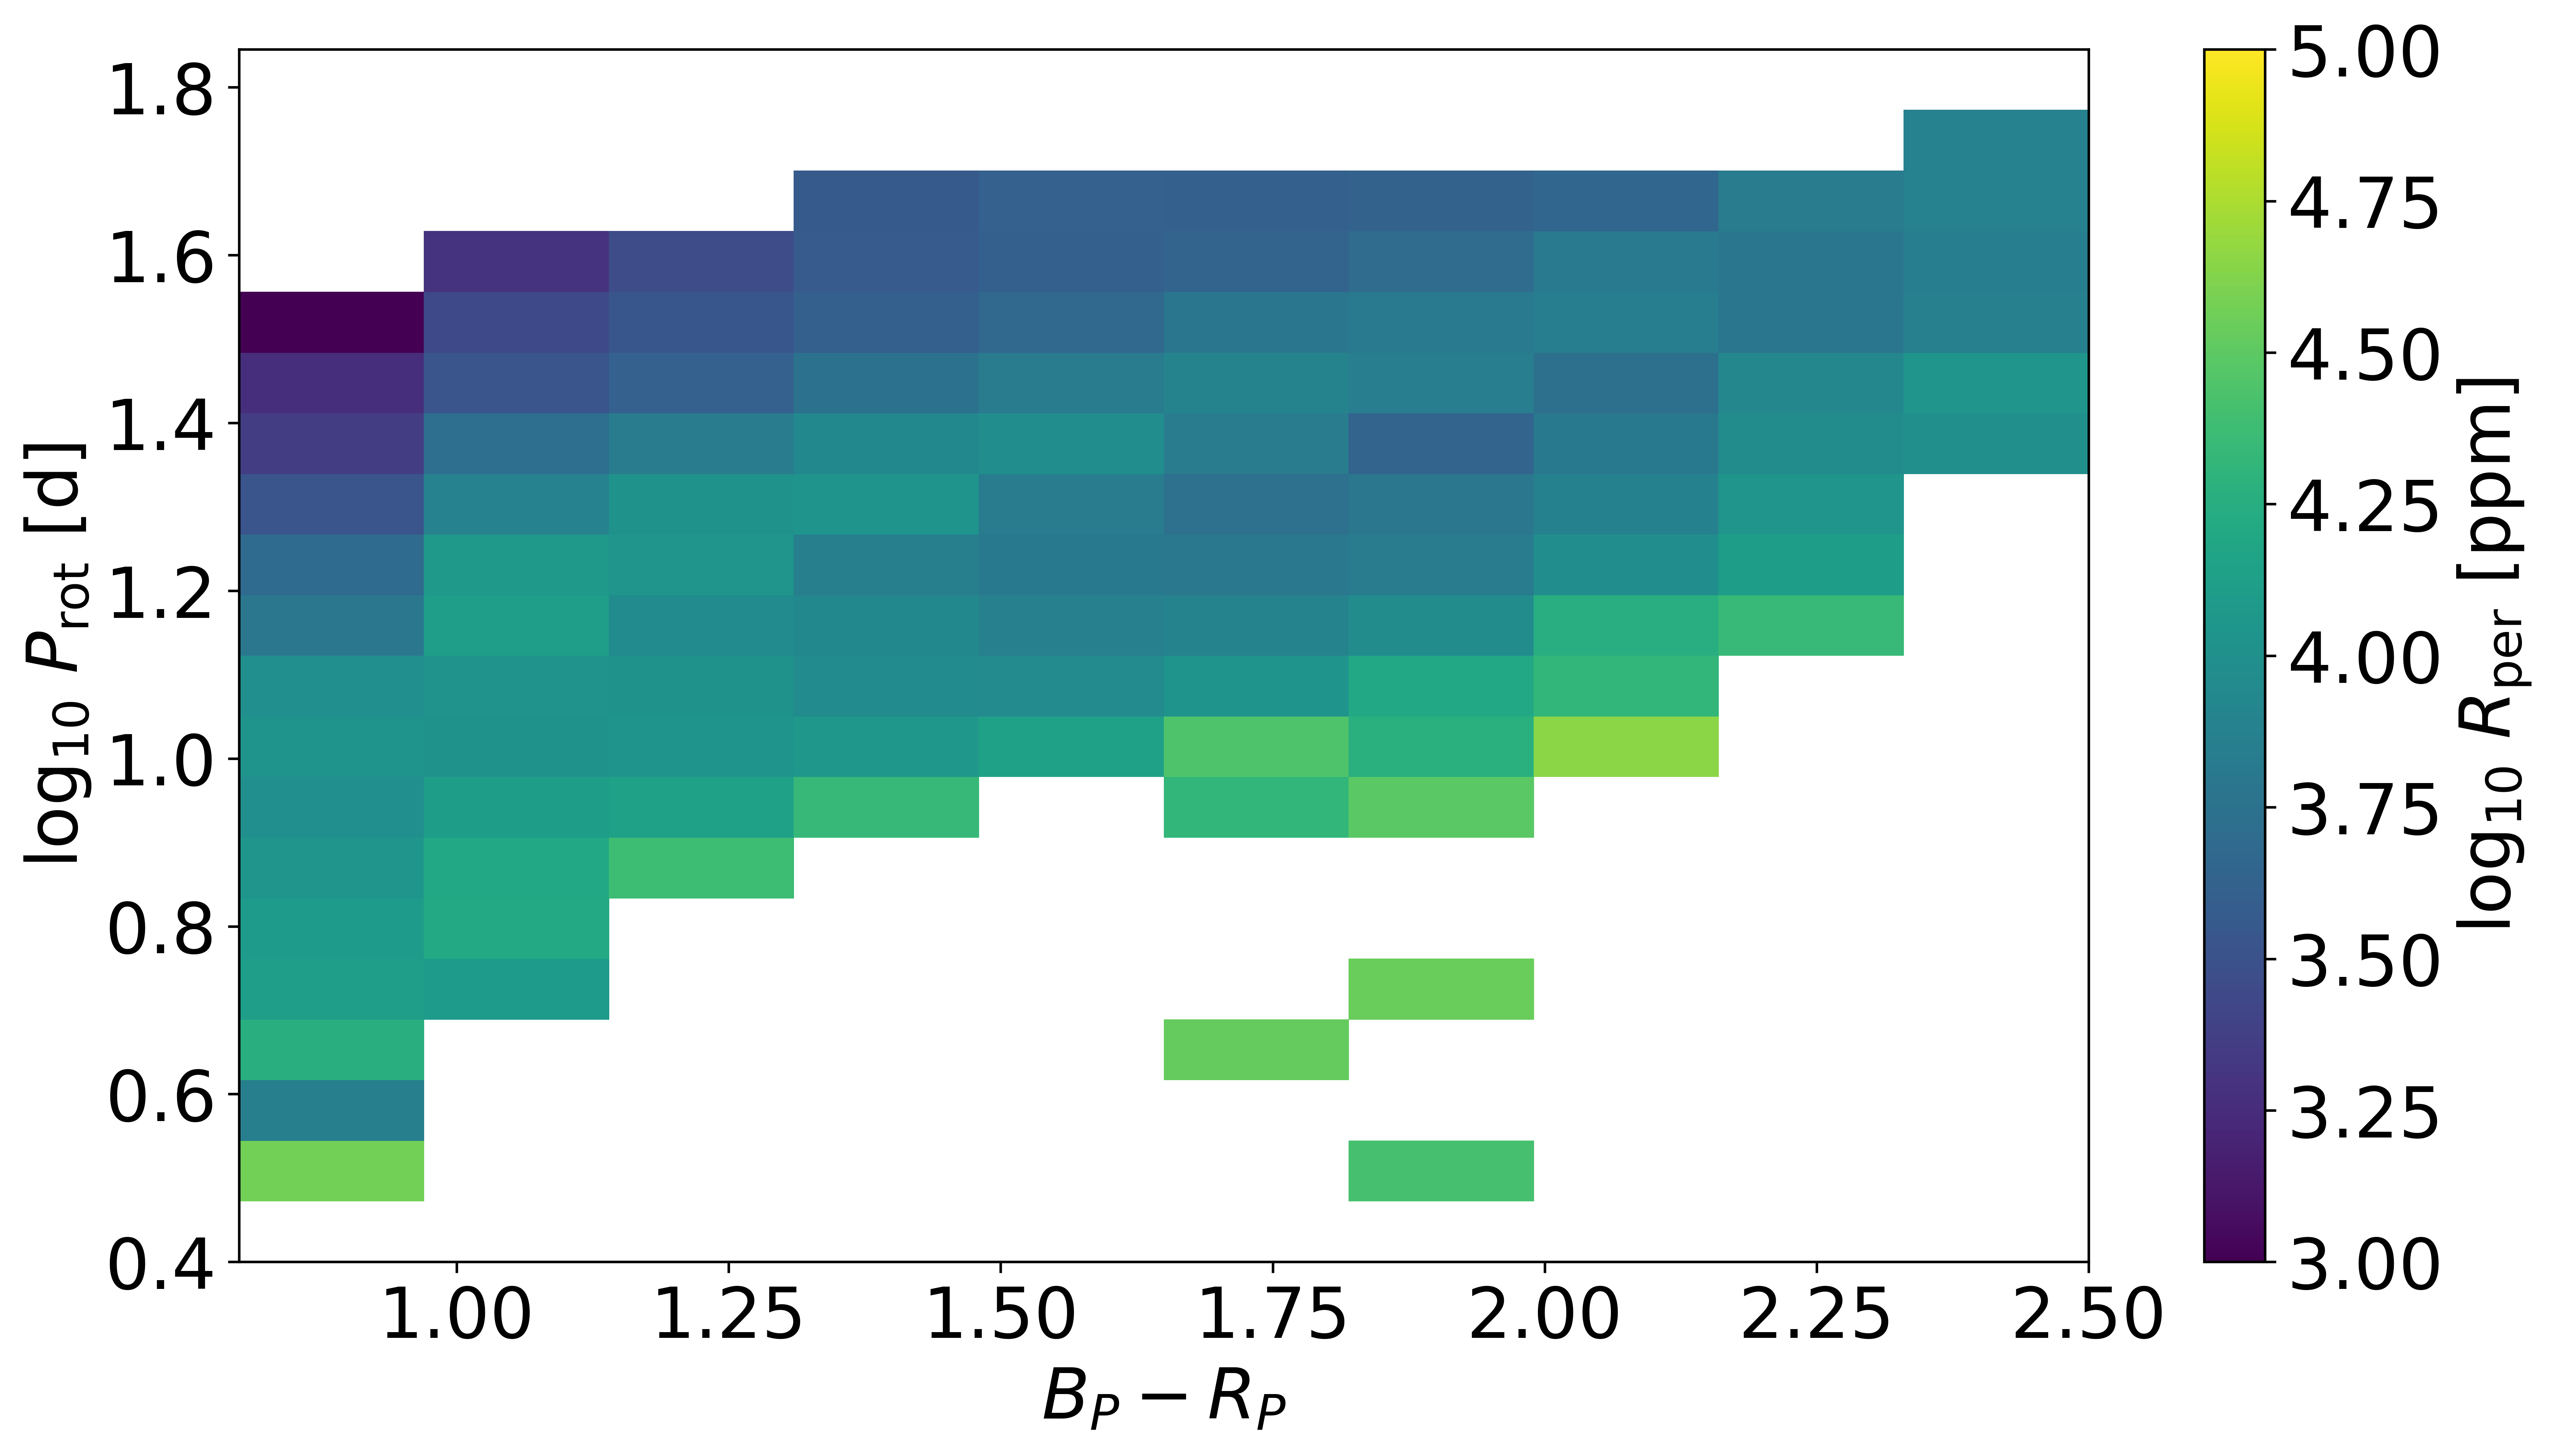
\includegraphics[width=\textwidth]{Figures/rot_gap_figures/rot_dist_binned.png}
  \caption[2D binned photometric variability (\rper{}) for the slices of $\log_{10}$ of the rotation period and colour \gaia{} $B_P-R_P$ used in this work.]{
  2D binned photometric variability (\rper{}) for the slices of $\log_{10}$ of the rotation period and colour \gaia{} $B_P-R_P$ used in this work. Comparing this Figure and \ref{fig:prawn}, the alignment of the minima of photometric variability and observation of stars in the gap can be seen.}
  \label{fig:binned_rper_full_sample}
\end{figure}

As a result of the large-scale variability with stellar mass and rotational period, the position of the minima becomes harder to notice as $B_P - R_P$ approaches 0.8.
We plot the same data in Figure \ref{fig:binned_rper_scatter} to make the minima more prominent.
We show the median \rper{} (scatter points) and scatter (errorbars) against the $\log_{10}$ of the rotation period for each colour range indicated in brackets - here, the colour of the interval increases down the plot - as well as fitted cubic spline to the data (dashed).
From the cubic spline, we can use the first and second derivatives of the spline to accurately determine the position of the local minima in \rper{}, which is indicated by the solid vertical blue line.

The calculation of the position of the minima is an automated process.
To identify minima, we calculate the first and second derivatives of the cubic spline fit and find where the first derivative is close to zero and where the second derivative is greater than 5 to ensure we ignore any spurious jitter in the spline fit.
We use an automated process to ensure we have not selected a position that we believe aligns with the intermediate period gap.
We found that the resulting position of minima can vary slightly depending on the smoothing of the cubic spline and the threshold value chosen for the second derivative.
However, the found minima here tended to be robust to variations of the smoothing at that threshold.
The first minima, in regards to the rotational period, in the $B_P-R_P =$ (0.8-0.97) bin was also manually ignored.

The position of the minima are shown in blue in Figure \ref{fig:indicating_minima}, where it is clear that the majority of minima align with the intermediate period gap.
We note that the minima do not accurately predict the position of the intermediate period gap for $B_P-R_P \geq 2.16$.
We believe this is because of the small number of stars below the gap in this colour range which were cut due to them not containing enough stars.
 With larger numbers of observations of low-mass stars below the gap we believe our prediction of the position of the rotation period gap with \rper{} \ would be more accurate in this regime. 
We also note that the average photometric modulation amplitude tends to peak to a maximum with a larger \rper{} than stars on the lower prong of the rotational period gap despite having longer rotation periods.
Whether this peak is indicative of stronger photometric activity suddenly above the gap or of suppression of photometric activity below the gap is unknown.

\begin{figure}
\centering
  \includegraphics[width=0.5\textwidth]{Figures/rot_gap_figures/rot_vs_rper_minima.png}
  \caption[Median and median absolute deviation of photometric variability (\rper{}) against $\log_{10}$ of the rotation period in bins of and colour \gaia{} $B_P-R_P$.]{
  Median and median absolute deviation of photometric variability (\rper{}) against $\log_{10}$ of the rotation period in bins of and colour \gaia{} $B_P-R_P$ (indicated in brackets). Here we have fitted a cubic spline to median \rper{} \ and calculated minima using the first and second derivatives of the fitted cubic spline. Solid vertical blue lines show the minima here. These minima align with the rotational period gap.}
  \label{fig:binned_rper_scatter}
\end{figure}

\begin{figure}
\centering
  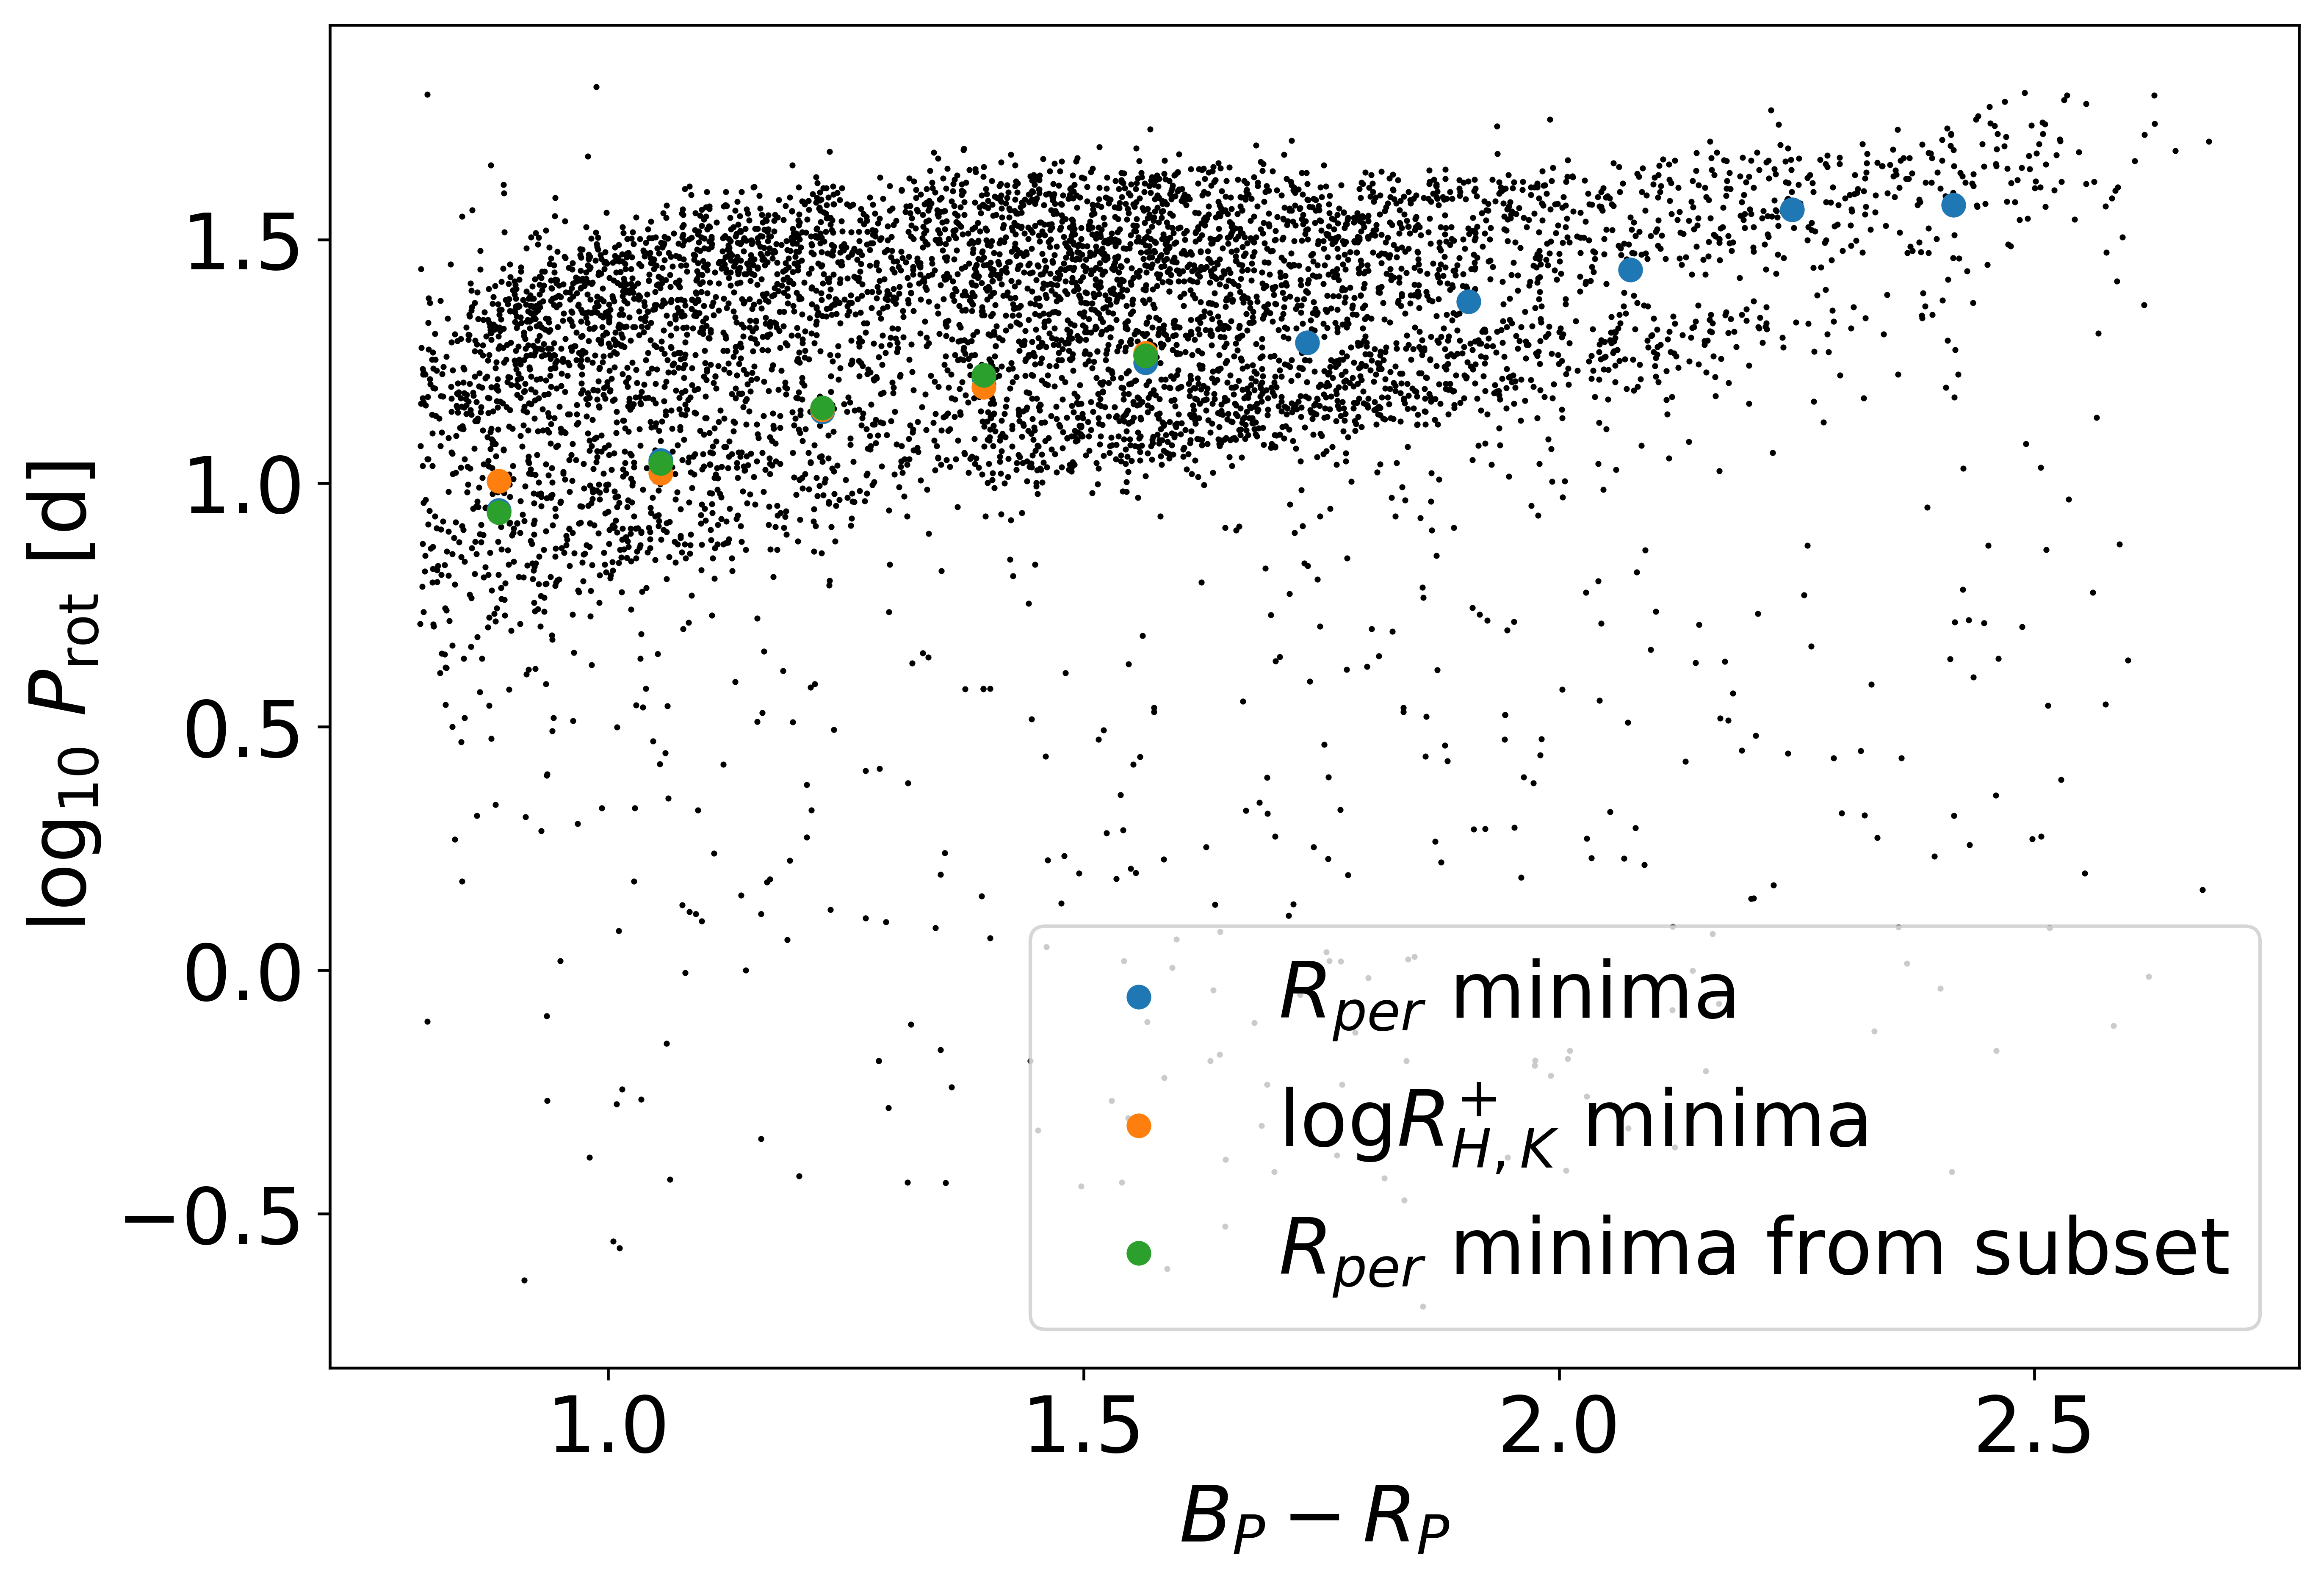
\includegraphics[width=\textwidth]{Figures/rot_gap_figures/rot_dist_minima_shown.png}
  \caption[The position of the identified minima in \rper{} \ against rotational period using the full close-by rotating main-sequence \kepler{} sample, the \rper{} minima identified with the \kepler-\lamost\ crossmatch and the $\log_{10} R^{+}_{H,K}$ minima identified with the \kepler{} \lamost\ crossmatch.]{
  The position of the identified minima in \rper{} \ against rotational period using the full close-by rotating main-sequence \kepler{} sample, the \rper{} minima identified with the \lamost\ crossmatch and the $\log_{10} R^{+}_{H,K}$ minima identified with the \kepler-\lamost\ crossmatch.}
  \label{fig:indicating_minima}
\end{figure}

A possible explanation for the decrease in median photometric variability comes from the nature of a dearth of observations, as the gap is not horizontally aligned and increases in period for stars of lower mass (higher $B_P-R_P$).
\rper{} generally decreases with mass and rotation period.
Taking the median value in slices of constant rotation period near the dearth of observations will be systematically biased in different ways as it passes through the dearth.
In order of increasing rotation period, a sample of stars in each bin of rotation period will contain initially, majority fast rotating but redder stars and a small number of slow-rotating bluer stars, then approximately equal fast-rotating red stars and slow-rotating blue stars, and finally majority slow-rotating bluer stars and a small number of fast-rotating redder stars.
The relationship between the \rper{} and mass or rotation period are not easily parameterised, especially near the gap.
However, we can confirm that this effect does not skew our results by calculating the median and median absolute deviation of $B_P-R_P$ in each colour and rotational period bin.
We have shown this in Figure \ref{fig:colour_rper}.
We confirm that the minima and maxima of \rper{} with rotation period in each colour bin do not correspond to minima or maxima in colour that would indicate that this effect is at play.
The variation is \rper{} is, therefore, a physical effect that aligns itself with the rotational period gap.

\begin{figure}
\centering
  \includegraphics[width=0.5\textwidth]{Figures/rot_gap_figures/per_vs_colour.png}
  \caption[Median and median absolute deviation of photometric variability (\rper{}) (blue) and $B_P-R_P$ (orange) against $\log_{10}$ of the rotation period in bins of and \gaia{} $B_P-R_P$ colour.]{
  Median and median absolute deviation of photometric variability (\rper{}) (blue) and $B_P-R_P$ (orange) against $\log_{10}$ of the rotation period in bins of and \gaia{} $B_P-R_P$ colour (indicated in brackets). The position of the minima in \rper{} \ do not align with maxima or minima in $B_P-R_P$ implying that the colour bias when fitting across the dearth can be the cause of the \rper{} \ minima.}
  \label{fig:colour_rper}
\end{figure}

At first glance, the minima in \rper{} surrounding the gap suggests that the rotation period gap is the result of the decreased probability of observing stars at the given rotation period.
However, the minima values of \rper{} within the gap can otherwise be detected for other colour stars.
For example, the minima in the $B_P-R_P$ -- (0.97-1.14) slice has a \rper{} value of $\sim 4.0$, which can otherwise be easily detected for slower rotating or redder stars.
This either suggests that the periodic variability drops suddenly to levels where rotation is not measurable at the rotation period gap or that the rotational variability drops due to the process by which stars cross the gap. 
 \citet{santos_surface_2021} increased the sensitivity of period detection for \kepler{} lightcurves and did not increase the number of stars observed near the intermediate period gap suggesting that the drop in photometric variability does not result in a decreased probability of observing stars near the gap.
This implies that if the drop in photometric variability is not the cause for the dearth of observations near the rotational period gap and rather that the drop in photometric variability is purely coincident with the rotational period gap - suggesting that the mechanism underlying the two observations is the same.
\rper{} is not defined for stars where rotation is not detected - as \rper{} is defined by the photometric variability range over a rotational period timescale.
Therefore we do not know whether the potential stars that lay within the gap, which we cannot observe because of the supposed dramatic decrease in \rper{}, do or do not suddenly decrease in \rper{}.

\section{The gap aligns with a minima in $\log R^{+}_{\rm{HK}}$ }
\label{sec:minima_rhk}

While it has been well established that the photometric variability of stars decreases towards the intermediate period gap, other magnetic activity indicators have not been explored in this regard, only the large-scale trends with stellar mass and rotation \citep{zhang_magnetic_2020}.
Suppose other magnetic activity indicators vary in the same fashion as \rper{} - decreasing to a minimum at the rotational period gap. 
In that case, it is more likely that the decrease in \rper{} towards the gap results from a variation in the magnetic field of stars.

\citet{zhang_magnetic_2020} extracted the chromospheric magnetic activity indexes, S and $\log \ R^{+}_{HK}$, for 59,816 stars from low-resolution \lamost\ spectra in the \kepler-\lamost\ crossmatch.
The crossmatch of their work with the nearby rotating main-sequence we established yielded 1060 stars.
The stars in the crossmatch tend to be the higher mass, brighter stars with $B_P-R_P<1.8$, where the intermediate period gap is less apparent.
Given that we could predict the gap position for these stars in our earlier experiment, we carry forward and re-analyse their data under a new framework.

$\log \ R^{+}_{HK}$ provides a more accurate measure of the chromospheric magnetic activity than $S$ so we adopt $\log \ R^{+}_{HK}$ in this work.
The resulting rotational distribution of stars is shown in Figure \ref{fig:rot_dist_rhk} coloured by $\log \ R^{+}_{HK}$.

\begin{figure}
\centering
  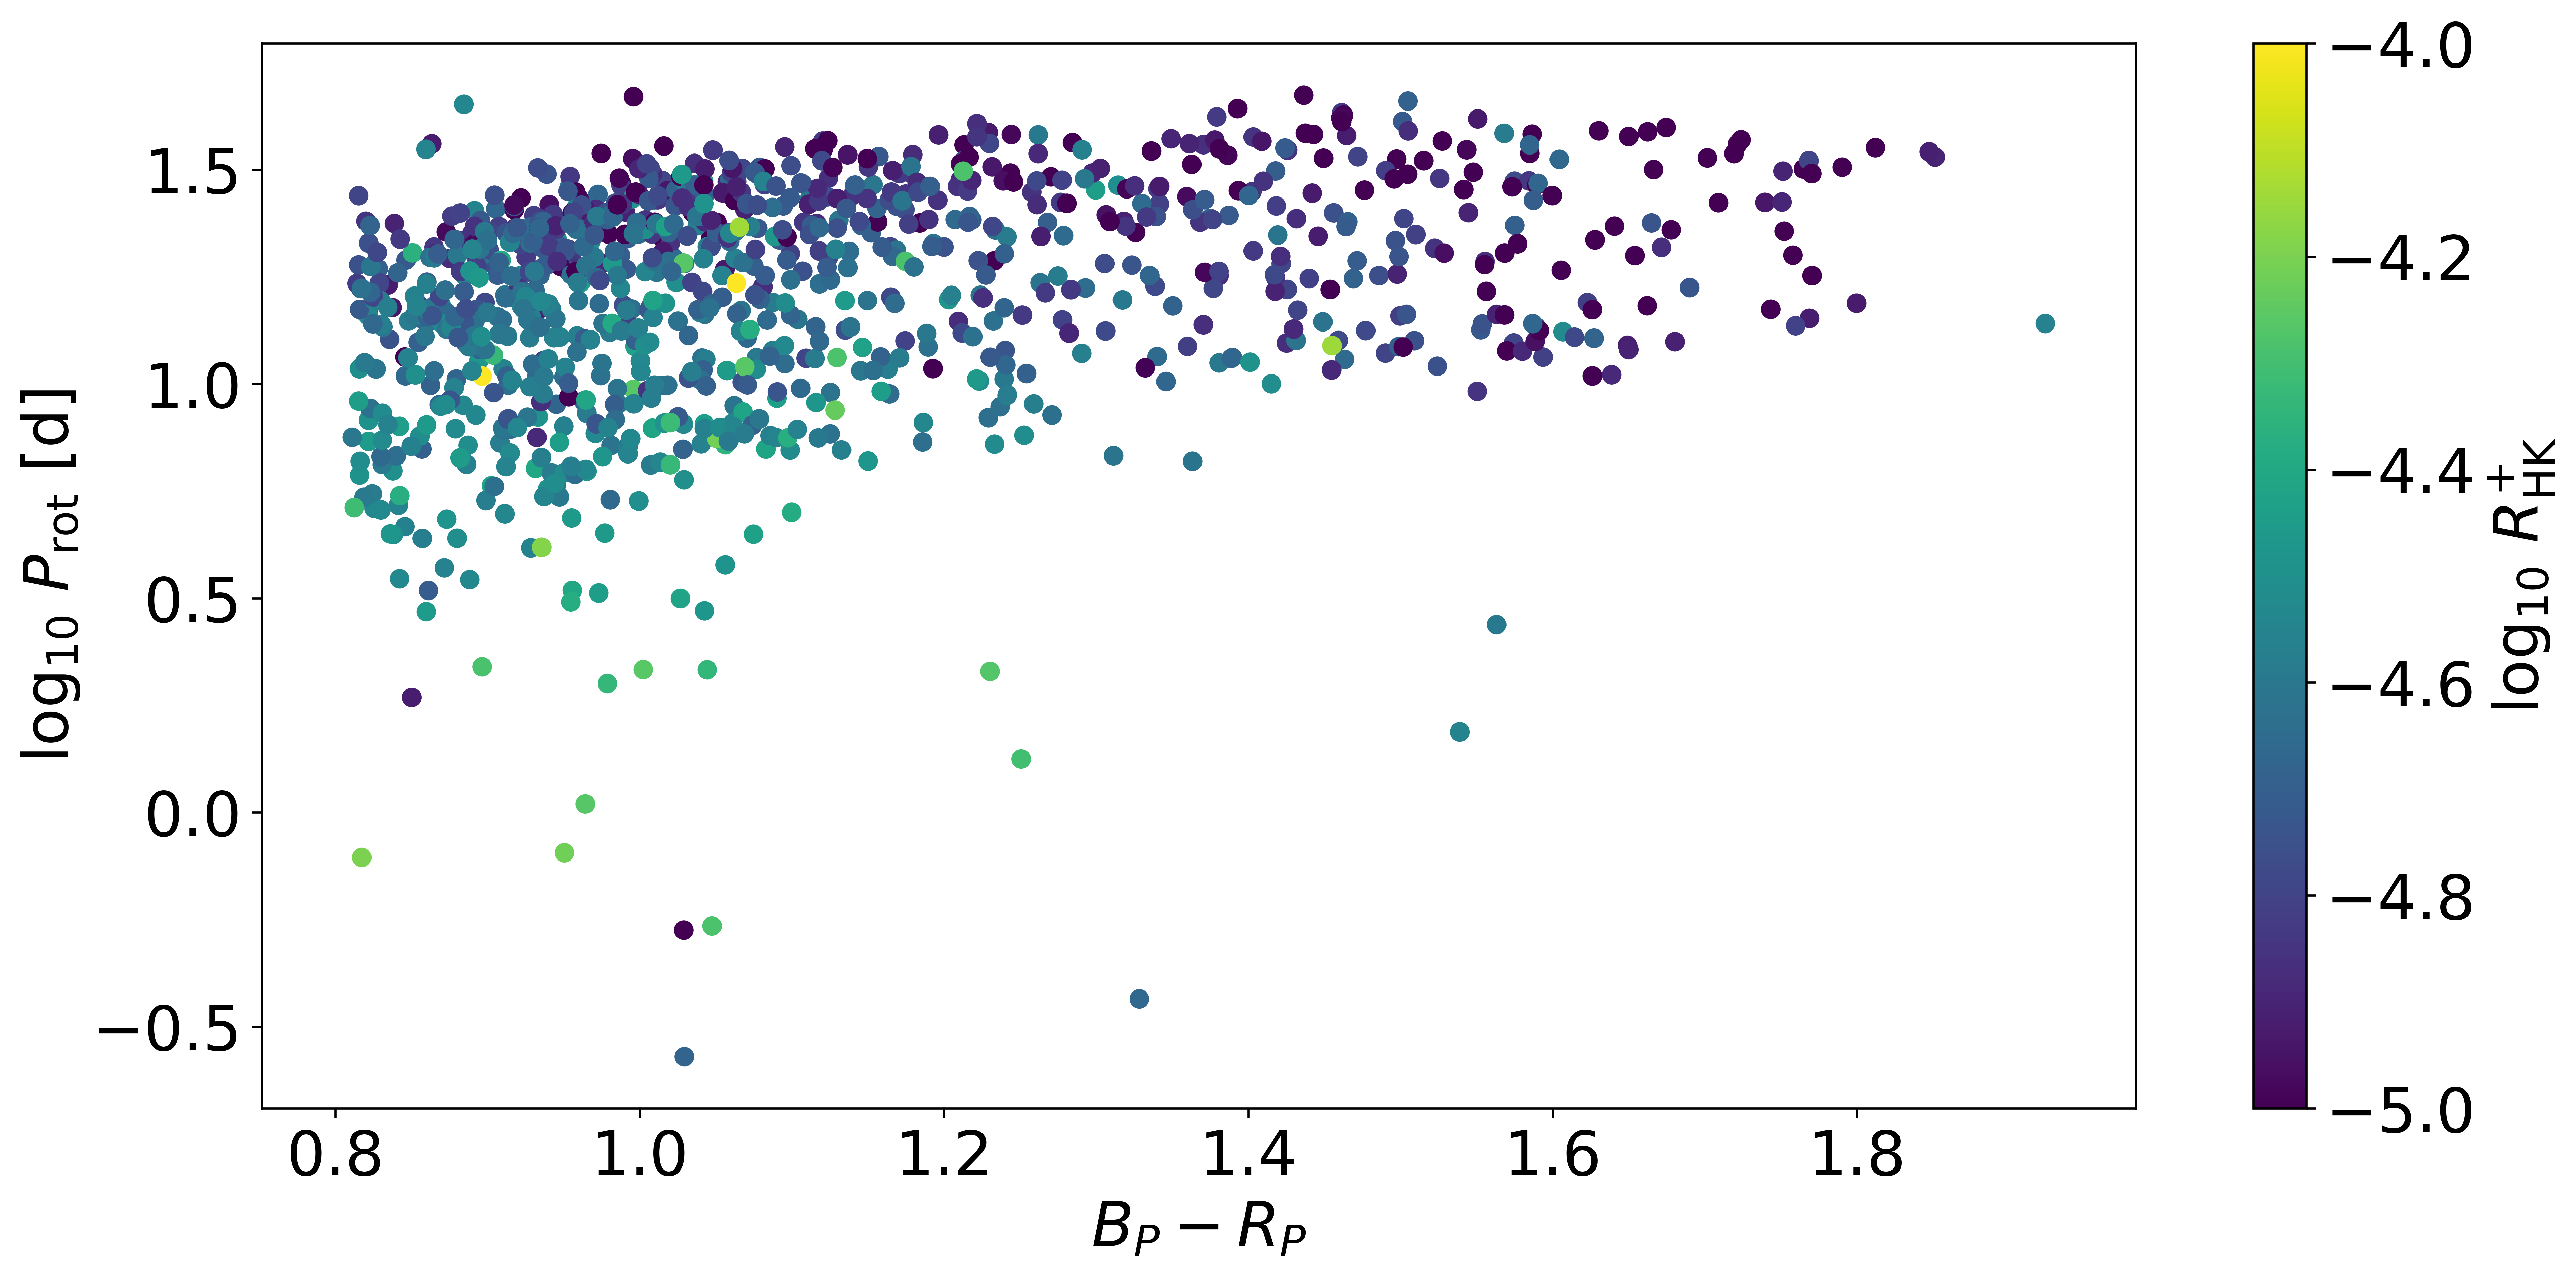
\includegraphics[width=\textwidth]{Figures/rot_gap_figures/rotational_dist_rhk.png}
  \caption[The \lamost\ chromospherically active and \kepler{} rotating closeby, main-sequence cross-match $\log_{10}$ of rotational period $\log_{10}$ against \gaia $B_P-R_P$ colour coloured by $\log_{10}R^{+}_{\rm{HK}}$.]{
  The \lamost\ chromospherically active and \kepler{} rotating closeby, main-sequence cross-match $\log_{10}$ of rotational period $\log_{10}$ against \gaia $B_P-R_P$ colour coloured by $\log_{10}R^{+}_{\rm{HK}}$. It is unclear from this whether $\log_{10}R^{+}_{\rm{HK}}$ decreases toward the gap like \rper{}.}
  \label{fig:rot_dist_rhk}
\end{figure}

We adopt the same process as we described earlier to find the minima in \rper{} \ in a bin of colour against the rotational period.
We again separate the stars into the same slices of $B_P-R_P$ and log of rotation period, and remove any bins containing small numbers of stars ($<$ 2).
This cut-off was chosen because of the reduced number of stars in the sample \kepler-\lamost\ crossmatch, compared to the \citet{mcquillan_rotation_2014} sample.
 Still, the results should be treated with more caution because we rely on small number statistics.
The median and median absolute deviation of both $\log \ R^{+}_{HK}$ and \rper{} \ in these slices was then calculated, which we then fit with cubic splines against the log of the rotation period.
We have repeated this method on \rper{} \ here because we are using a subset of the original stars and to compare the recovered minima from the subset more accurately this also allows us to confirm the accuracy of the fit of our minima in the first test.
The minima of the cubic spline fits are then calculated again using the first and second derivatives using the same smoothing and first and second derivative thresholds.

\begin{figure}
\centering
  \includegraphics[width=\textwidth]{Figures/rot_gap_figures/rot_vs_rper_rhk_minima.png}
  \caption[Median and median absolute deviation of photometric variability (\rper{}) (blue) and \lamost\ $\log_{10}R^{+}_{\rm{HK}}$ against $\log_{10}$ of the rotation period in bins of and colour \gaia{} $B_P-R_P$.]{
  Median and median absolute deviation of photometric variability (\rper{}) (blue) and \lamost\ $\log_{10}R^{+}_{\rm{HK}}$ against $\log_{10}$ of the rotation period in bins of and colour \gaia{} $B_P-R_P$ (indicated in brackets). Here we have fitted a cubic spline to the median of these values in each bin and calculated minima using the first and second derivatives of the fitted cubic spline. The minima in \rper{} are shown by solid vertical blue lines, while the minima in $\log_{10}R^{+}_{\rm{HK}}$ are shown in solid vertical orange lines. These minima align with each other and the rotational period gap.}
  \label{fig:rot_rper_rhk}
\end{figure}

We compare the distributions of \rper{} \ and $\log \ R^{+}_{HK}$ against the log of rotation period in Figure \ref{fig:rot_rper_rhk} and show the found minima in blue and orange solid vertical lines for \rper{} \ and $\log \ R^{+}_{HK}$ respectively.
Like photometric variability, $\log \ R^{+}_{HK}$ tends to decrease with rotational period owing to their relation to the strength of the magnetic field.
We find that, generally, \rper{} \ and $\log \ R^{+}_{HK}$ are directly tied: increases and decreases to the median value with rotational period in one tends to align with a similar response in the other.

We show the comparison of the recovered minima from \rper{} using this subset as well as the minima recovered using $\log \ R^{+}_{HK}$ in Figure \ref{fig:indicating_minima}.
The recovered \rper{} \ minima using the subset lay on top of the \rper{} minima recovered using the full sample.
Interestingly, we may detect previously unreported minima in $\log \ R^{+}_{HK}$ close to the rotation period gap.
Excluding the minima recovered in the $B_P-R_P$ - (0.8-0.97) bins, the minima that we recover in $\log \ R^{+}_{HK}$ against logged rotational period are in the same period bin and are close in position to the minima of \rper{} we recover, which we have established aligns with the intermediate period gap.
The alignment of the minima is also robust to variation in the smoothness of the fitted cubic spline - suggesting that the minima are not spurious.

Measurements of $\log \ R^{+}_{HK}$ are less precise than \rper{}.
The detection of the coincidence in a single slice of $B_P-R_P$ could be explained through this imprecision.
Detecting this in multiple slices of $B_P-R_P$ suggests that the cause of the minima is related.
We will assume, for now, that the rotational period gap does align itself with minima in both \rper{} and $\log \ R^{+}_{HK}$ and explore whether there is a sample of low-magnetic activity, non-detected rotators.

\section{Is there a sample of low-magnetic activity stars without rotational period detection?}
\label{sec:low_activity_gap}

If the gap contains stars that have dramatically low \rper{} and thus do not have detectable rotation periods, then $\log \ R^{+}_{HK}$ should also dramatically drop within this regime.
If there is a sample of dramatically lower $\log \ R^{+}_{HK}$ stars without detected rotation periods, then the existence of such a subsample would support the hypothesis that the intermediate period gap results from a decreased probability of observing stars at those rotation periods due to a decrease in stellar activity.

%To determine whether a star has a significant rotational period detection \citet{mcquillan_rotation_2014} defines a weight of the significance of the detection of the rotational period $w$ and compares this to a threshold value.
%$w$ is defined in terms of the ACF's local peak height (LPH), the height of the selected peak with respect to the mean of the troughs on either side, the star's temperature and the rotational period.
%For a more thorough description of their method for calculating this value see Section A in the appendix of their work.
%This normalised value is calculated for each star and compared to a threshold value.
%Those that do not pass the threshold were placed into a separate category of stars that do not have a detectable rotation period.

We will compare the $\log \ R^{+}_{HK}$ distributions of the \citet{mcquillan_rotation_2014} rotating and non-rotating samples.
We prepare the sample of 99,000 stars without detected rotation periods from their work\footnote{This is a slight misnomer as \textit{some} of the stars $\sim$ 100,000 stars have detectable rotation periods, but do not pass a detectability threshold, see Section A in the appendix of their work, and those periods should be treated with some care.} in the same way that we did for the rotating sample ensuring they are close by ($<525 pc$), on the main-sequence and redder than $B_P-R_P$ = 0.8 where the rotational period gap is most apparent.
This leaves us with a sample of 5574 non-rotating close by, main-sequence stars, which we can cross match with the \kepler-\lamost\ sample of chromospheric active stars measured in \citet{zhang_magnetic_2020} reducing the number of stars to 1134 stars.
The number of stars in this sample is similar to that in the rotating sample.
We show the resulting HR diagram of stars without rotational detection (bottom) and with rotational detection (top) in Figure \ref{fig:non_rotating_mag_hr} coloured by $\log \ R^{+}_{HK}$.
Comparing the distributions, it is clear that the non-rotating sample is clearly biased for higher mass stars and does not permeate into the low mass regime, where the gap would be most apparent.

\begin{figure}
\centering
  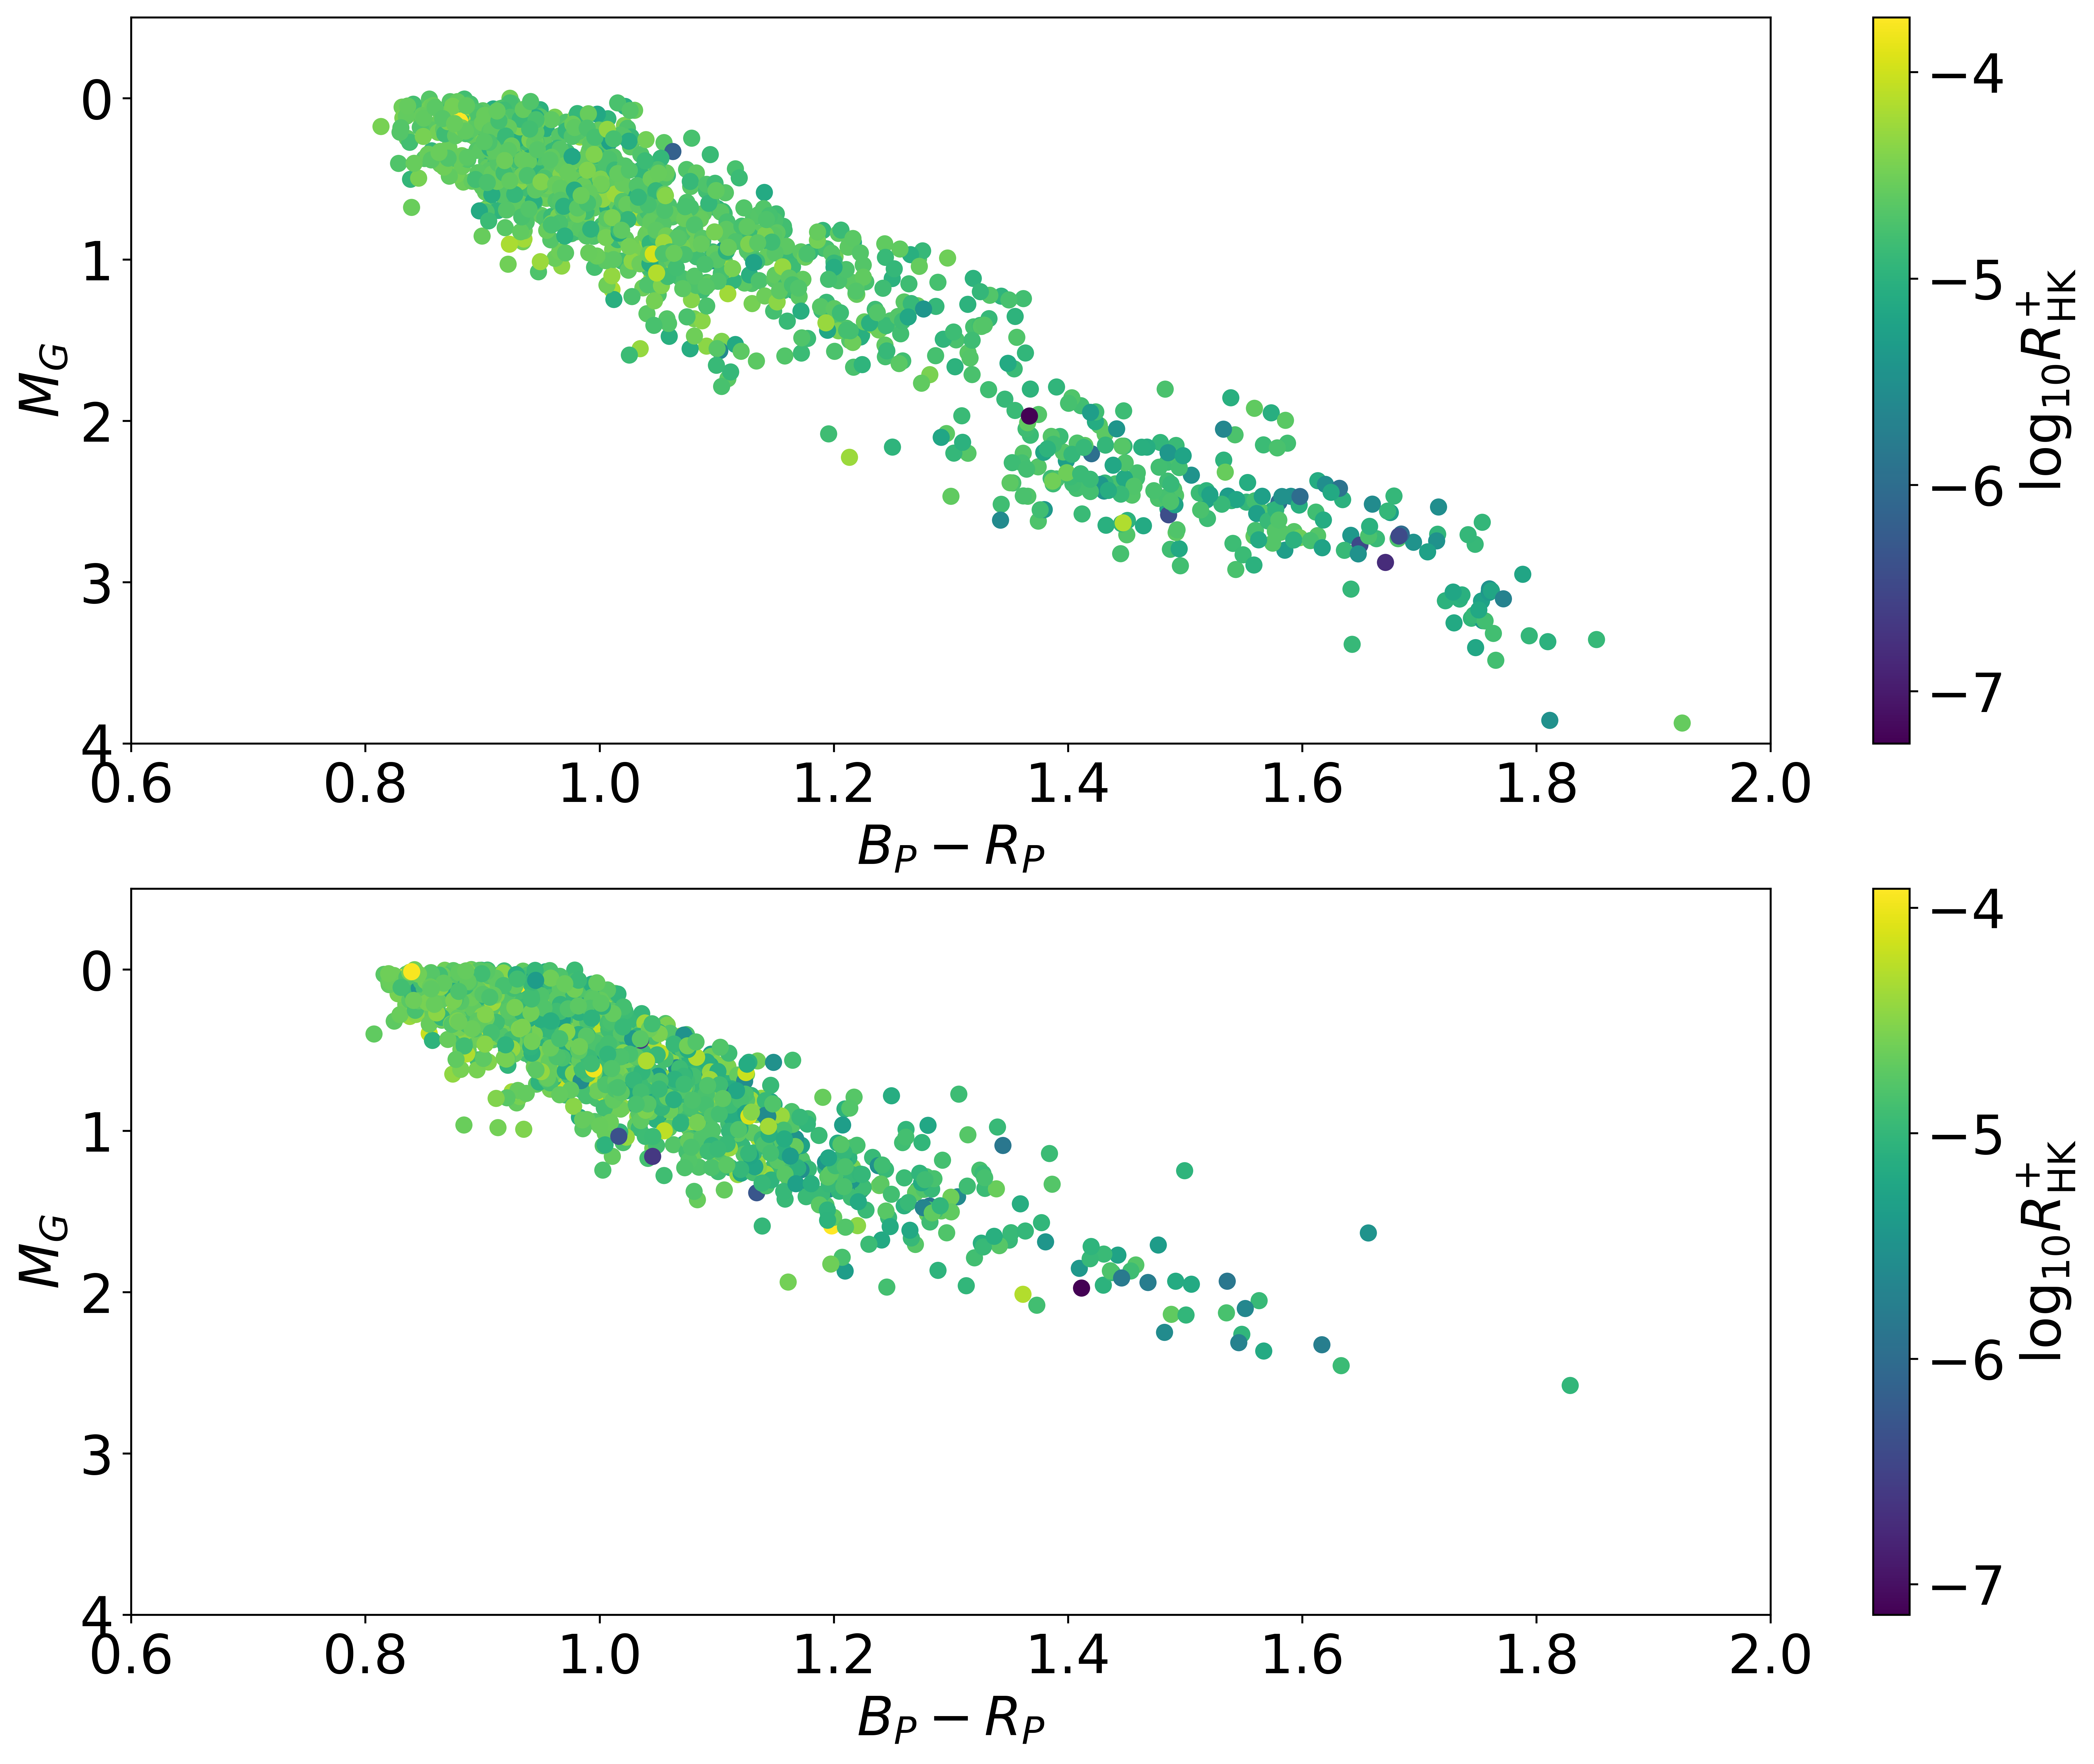
\includegraphics[width=\textwidth]{Figures/rot_gap_figures/HR_mag_and_non_rot.png}
  \caption[HR diagram of the closeby rotating (top) and non-rotating (bottom) main-sequence sample crossmatched with the \kepler-\lamost\ field coloured by the chromospheric magnetic activity indicator $\log \ R^{+}_{HK}$.]{
  HR diagram of the closeby rotating (top) and non-rotating (bottom) main-sequence sample crossmatched with the \kepler-\lamost\ field coloured by the chromospheric magnetic activity indicator $\log \ R^{+}_{HK}$.
  Comparing these two samples, we observe very few low-mass stars for which the rotation period is undetected.}
  \label{fig:non_rotating_mag_hr}
\end{figure}

With the rotating and non-rotating \kepler-\lamost\ samples we can investigate the detectability of rotation as a function of $\log \ R^{+}_{HK}$.
We expect more magnetically active stars (higher $\log \ R^{+}_{HK}$) to be easier to detect in rotation as \rper{} should increase in turn.
However, as we have noted earlier in this work, stars can have their rotation go undetected for a multitude of reasons and the non-detection of rotation will not purely be the result of lower magnetic activity.
Figure \ref{fig:pdf_cdf} shows the distribution of rotation detected and rotation non-detected samples with $\log \ R^{+}_{HK}$.
The left panel shows the probability density, while the right shows the cumulative probability density function.
Stars detected in rotation appear to have higher $\log \ R^{+}_{HK}$ than those without detection.
A Kolmogorov-Smirnov (KS) test returns a $p$-value of $4 \cdot10^{-15}$.
With this, we can reject the null hypothesis that the two samples are drawn from the same underlying distribution with strong statistical significance.
The non-rotation detected tends to be less magnetically active, in terms of $\log \ R^{+}_{HK}$, than the rotationally detected sample.
Less magnetically active stars to have a lower detection rate due to the decrease in prominence of stellar spots with lowering magnetic activity.

\begin{figure}
\centering
  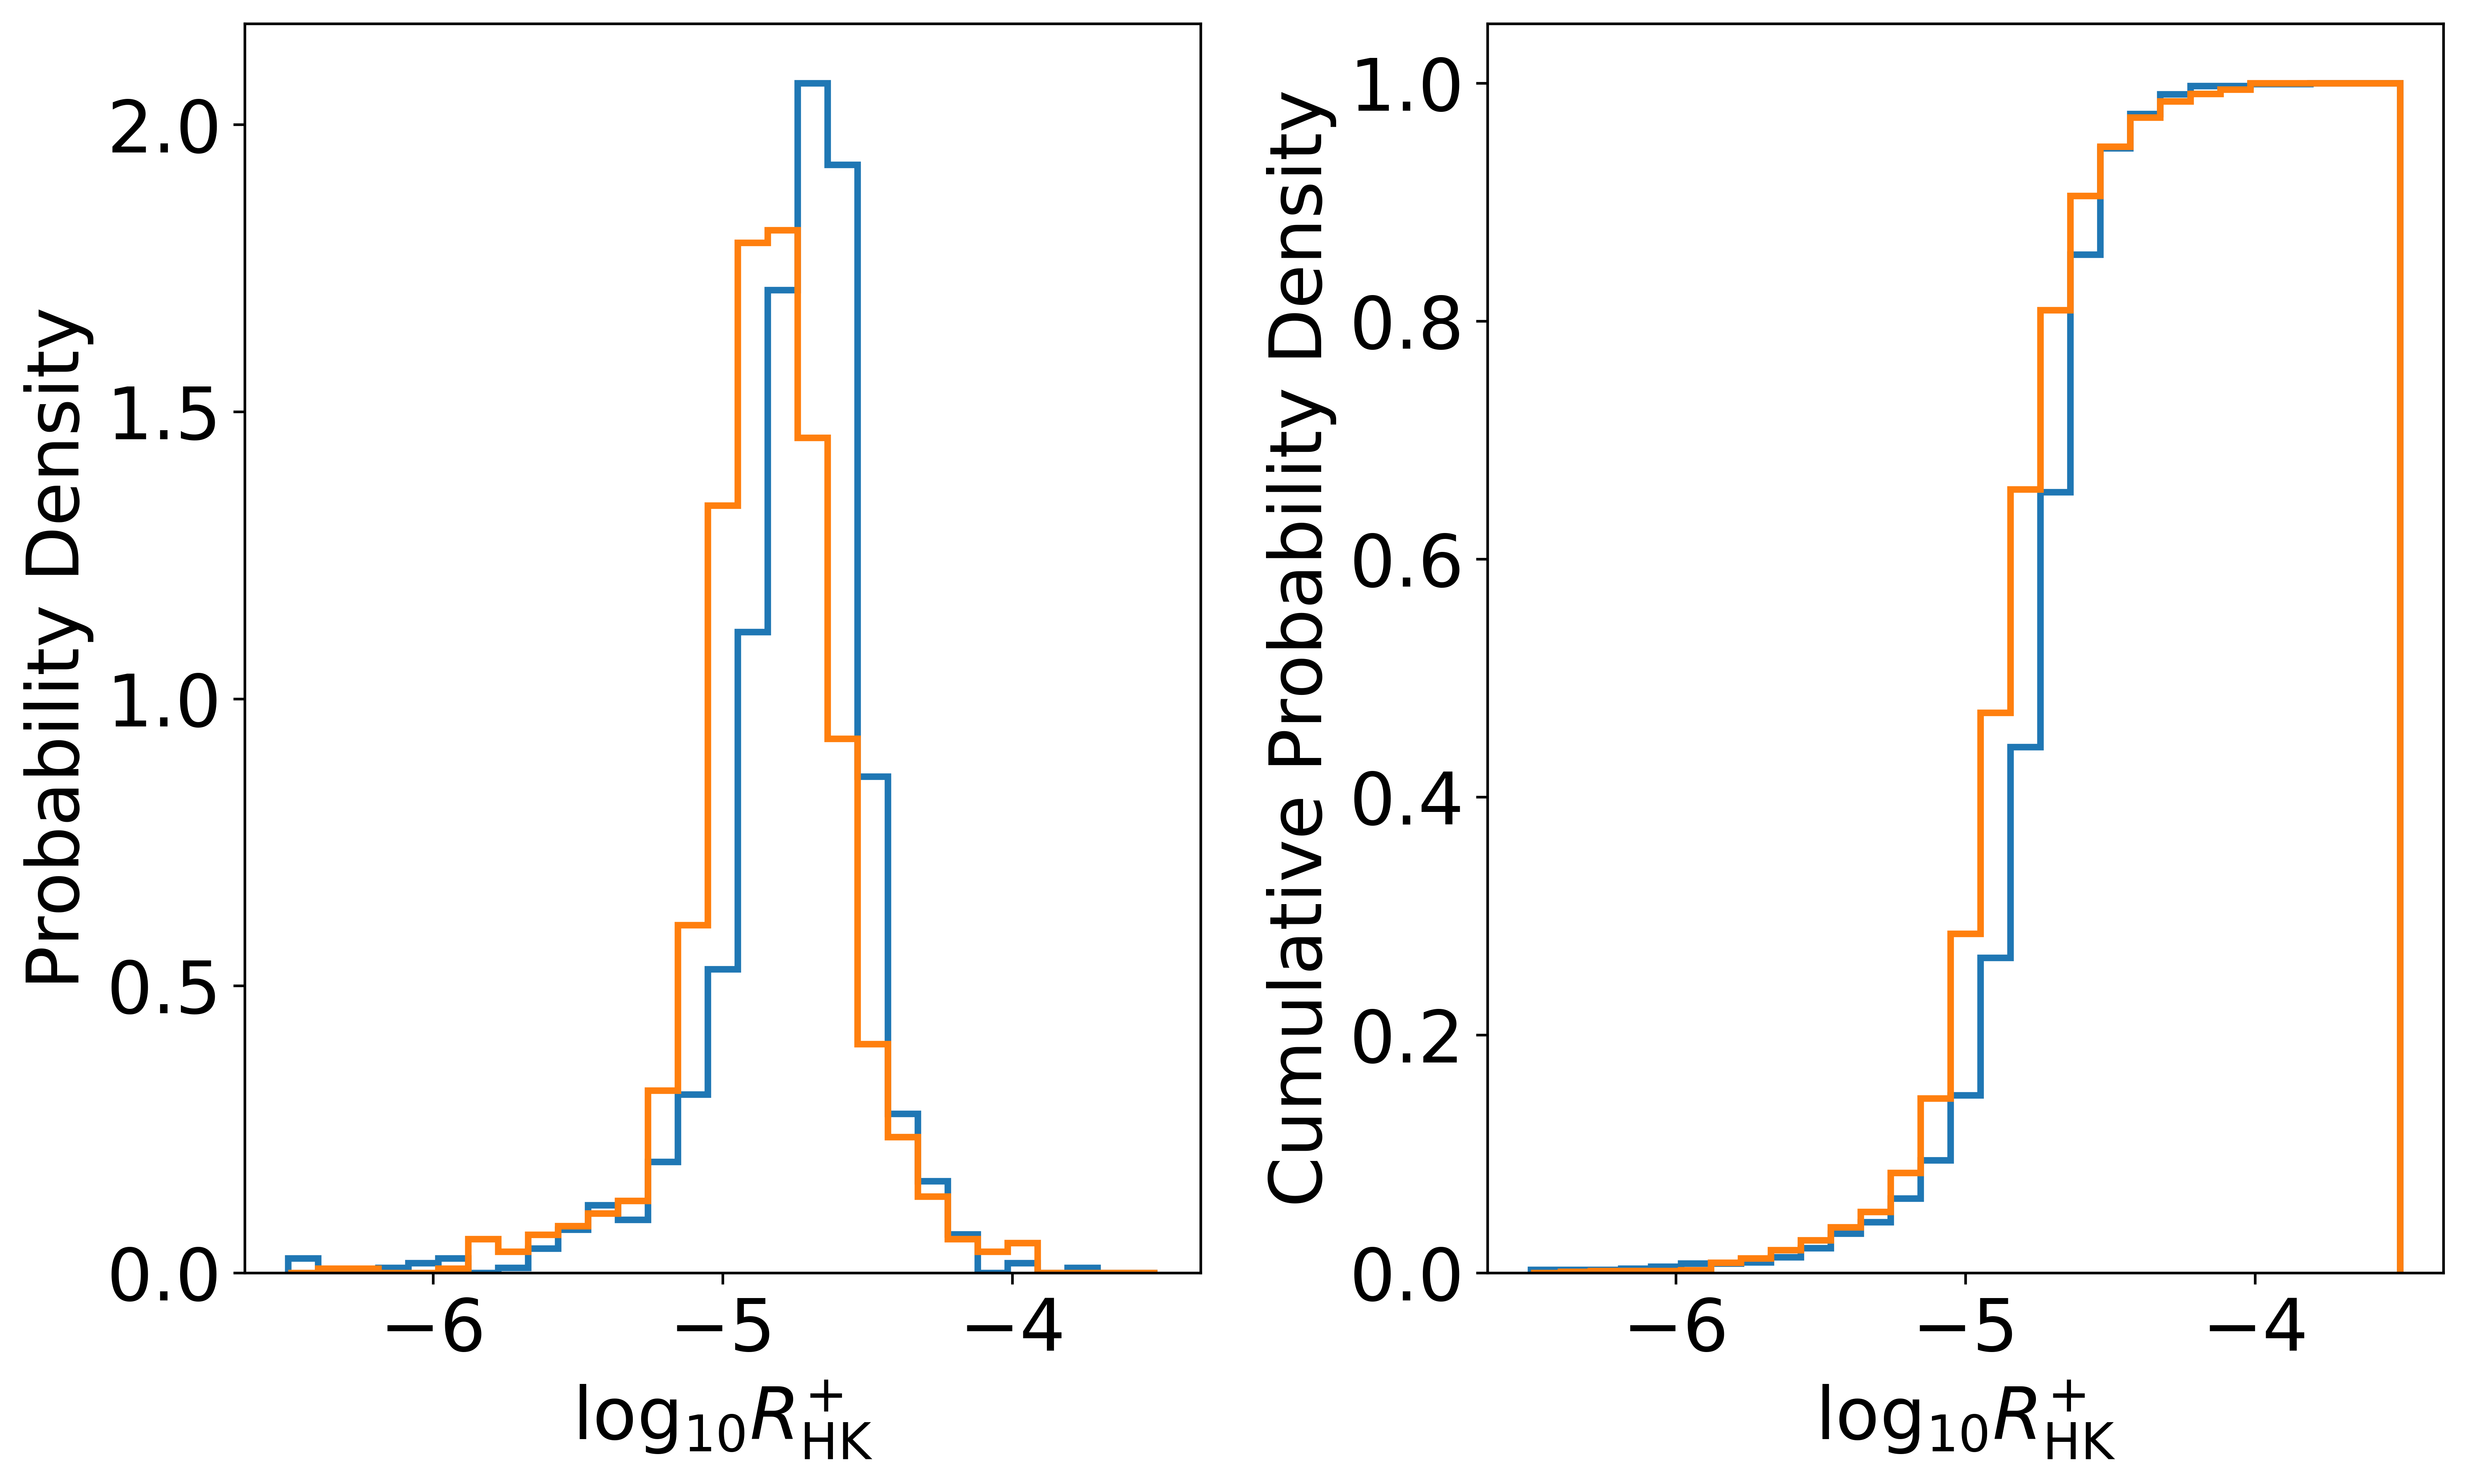
\includegraphics[width=\textwidth]{Figures/rot_gap_figures/pdf_cdf.png}
  \caption[The probability density function (left) and cumulative probability density function (right) of $\log \ R^{+}_{HK}$ are separated by whether rotation was (blue) or was not (orange) detected in the close-by main-sequence \kepler-\lamost\ crossmatch.]{
  	The probability density function (left) and cumulative probability density function (right) of $\log \ R^{+}_{HK}$ are separated by whether rotation was or was not detected in the close-by main-sequence \kepler-\lamost\ crossmatch. 
	We expect less magnetically active stars to have a lower detection rate due to the decrease in prominence of stellar spots with lowering magnetic activity.
 This is supported by the data here as the non-rotation detected sample contains a larger number of low $\log \ R^{+}_{HK}$ stars.}
  \label{fig:pdf_cdf}
\end{figure}

To investigate the detectability of rotation, let us consider the fraction of targets for which we detected periods in bins of colour and $\log \ R^{+}_{HK}$.
The detection efficiency here is measured from the ratio of the number of stars with a measured rotation rate to the total number of stars in that bin.
Other works \citep[see, e.g.,][]{claytor_tess_2023} consider the ratio of stars with highly precise rotation period measures to those without.
We forgo any cuts to the fractional error on the rotational period as we have limited our stars to nearby stars, which should have very high precision recovery of the stellar rotation period, and we also make no cuts to the number of stars in each bin that we calculate the histogram for. 
While limiting the minimum number of stars would allow us to clarify large-scale trends, we are searching for a subsample of stars with spuriously low magnetic activity with an already small sample size.

\begin{figure}
\centering
  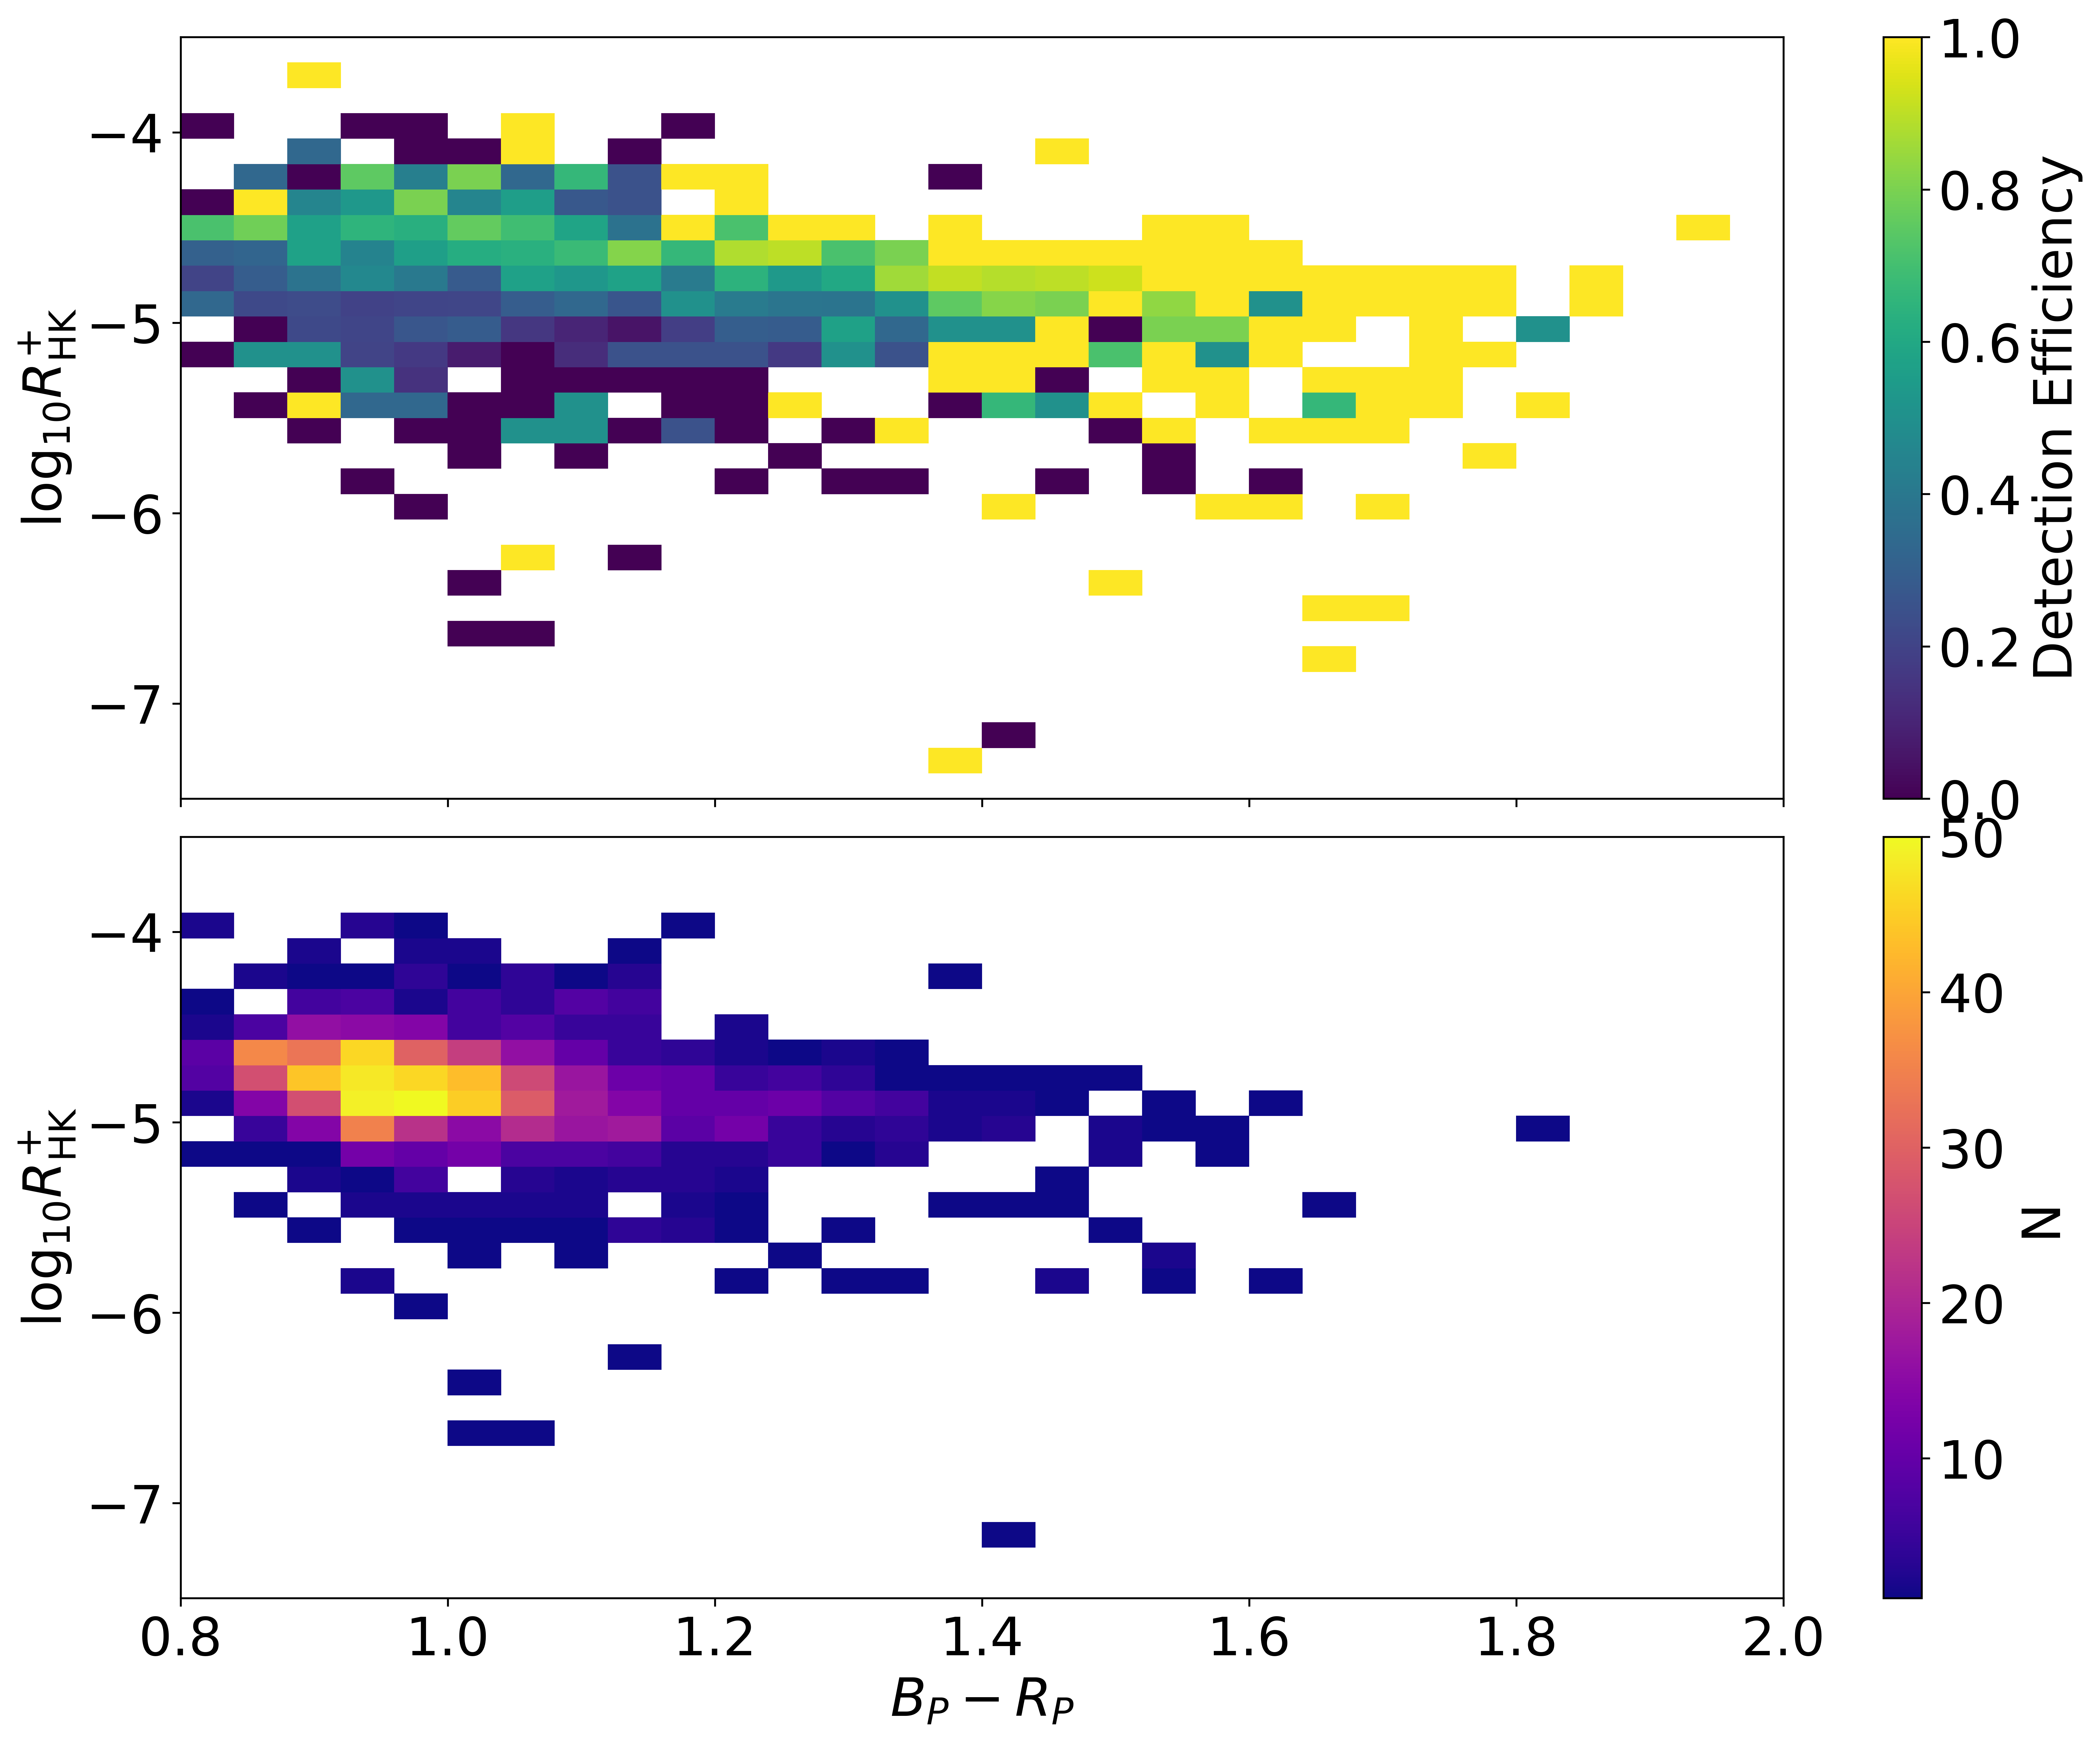
\includegraphics[width=\textwidth]{Figures/rot_gap_figures/detection_efficiency.png}
  \caption[The detectability of rotation (top) and 2D histogram of stars without detected rotation periods (bottom) across \gaia{} $B_P - R_P$ colour and $\log \ R^{+}_{HK}$.]{
  	The detectability of rotation (top) and 2D histogram of stars without detected rotation periods (bottom) across \gaia{} $B_P - R_P$ colour and $\log \ R^{+}_{HK}$. 
	Rotation is preferentially measured in stars with higher magnetic activity (larger $\log \ R^{+}_{HK}$) and tends to increase with colour. Low-mass stars have a high probability of rotation being measured. Stars with low magnetic activity have a lower likelihood of rotational observation. 
Bins with detection efficiency equal to zero or one tend to contain single stars, with detected rotation or without detected rotation, respectively and are not indicative of trends in the detection efficiency.
	We do not observe an ultra-low magnetic activity population with non-detected rotation that would be required to explain the lack of observation of stars in the intermediate period gap.
	While there are stars with ultra-low $\log \ R^{+}_{HK}$ ($<$5.5) in each $B_P-R_P$ bin they can either both rotationally detected or not rotationally detected. The ultra-low magnetic activity does not indicate their lack of rotational observation probability.
}
  \label{fig:detection_efficiency_rhk}
\end{figure}

Figure \ref{fig:detection_efficiency_rhk} shows the detection fraction (top) and a 2D histogram of the non-detected rotation sub-sample (bottom) against colour and $\log \ R^{+}_{HK}$. 
We confirm that rotation is preferentially measured in stars with higher magnetic activity (larger $\log \ R^{+}_{HK}$) and tends to increase with colour. 
Low-mass stars have a high probability of rotation being measured.
If we assume that stars of the same $\log \ R^{+}_{HK}$ express the same number of stellar spots, then dimmer stars will express larger variability, due to the larger change in relative flux from each spot, and thus will have a higher detectability of rotation.
We do not observe an ultra-low magnetic activity population with undetected rotation that would be required to explain the lack of observation of stars in the intermediate period gap.
While there is stars with low, for a given colour bin, and ultra low $\log \ R^{+}_{HK}$ ($<$5.5) in each $B_P-R_P$ bin, stars in those bins can both be rotationally detected or not rotationally detected. 
Ultra-low magnetic activity does not indicate their lack of probability of rotational observation, and there is no subsample of ultra-low magnetic activity stars without detected rotation periods.
While stars older-slowly rotating stars also tend to have lower $\log \ R^{+}_{HK}$, which may camouflage a population of low $\log \ R^{+}_{HK}$ gap stars, they still tend to have observable rotation periods.
For the gap to exist the magnetic activity would need to drop to a point where observation of rotation period is impossible, which is not supported by the data here.

\section{The lack of observation of stars that could fill the intermediate period gap}
\label{sec:no_gap_stars}

For the hypothesis that the gap represents a minimum of stellar rotational period detection and that the gap is indeed full of stars, then must be enough stars without detected rotation periods to fill the shortage of observations.
In this Section, we will determine whether this is indeed the case.

We will assume that the multiple missions that have observed the rotation period gap (\kepler, \ktoo, \ZTF, \tess) missions are not biased away from observing stars within the rotation period gap and compare the distribution of stars in the \citet{mcquillan_rotation_2014} \kepler{} rotating and undetected rotating samples.
Further, this analysis will focus on very low-mass stars where the gap is most apparent where \citet{mcquillan_rotation_2014} remains the state-of-the-art in detecting rotational periods for low-mass stars near the gap.
We make no quality cuts to the data to ensure we are not preferentially selecting for stars that could/could not possibly fill the gap.

If we compare the distribution of the number of stars in the rotation detected and undetected samples with colour, as we have shown in Figure \ref{fig:n_det_nondet}, we observe that stars with detectable rotation periods outnumber stars with undetectable rotation periods at lower masses ($B_P-R_P$ $\geq$1.3), despite the overall 3:1 ratio of the detectable rotation period to undetectable period catalogues.
In the inset of this Figure, where we compare the distributions where the gap is most apparent, we see that the proportion of stars with undetectable rotation periods to stars with detectable rotation periods decreases with decreasing mass, to a minimum of 1:10 undetectable to detectable rotation periods at the lowest masses.
This suggests that there are not a large number of stars available to fill the rotational period gap.

\begin{figure}
\centering
  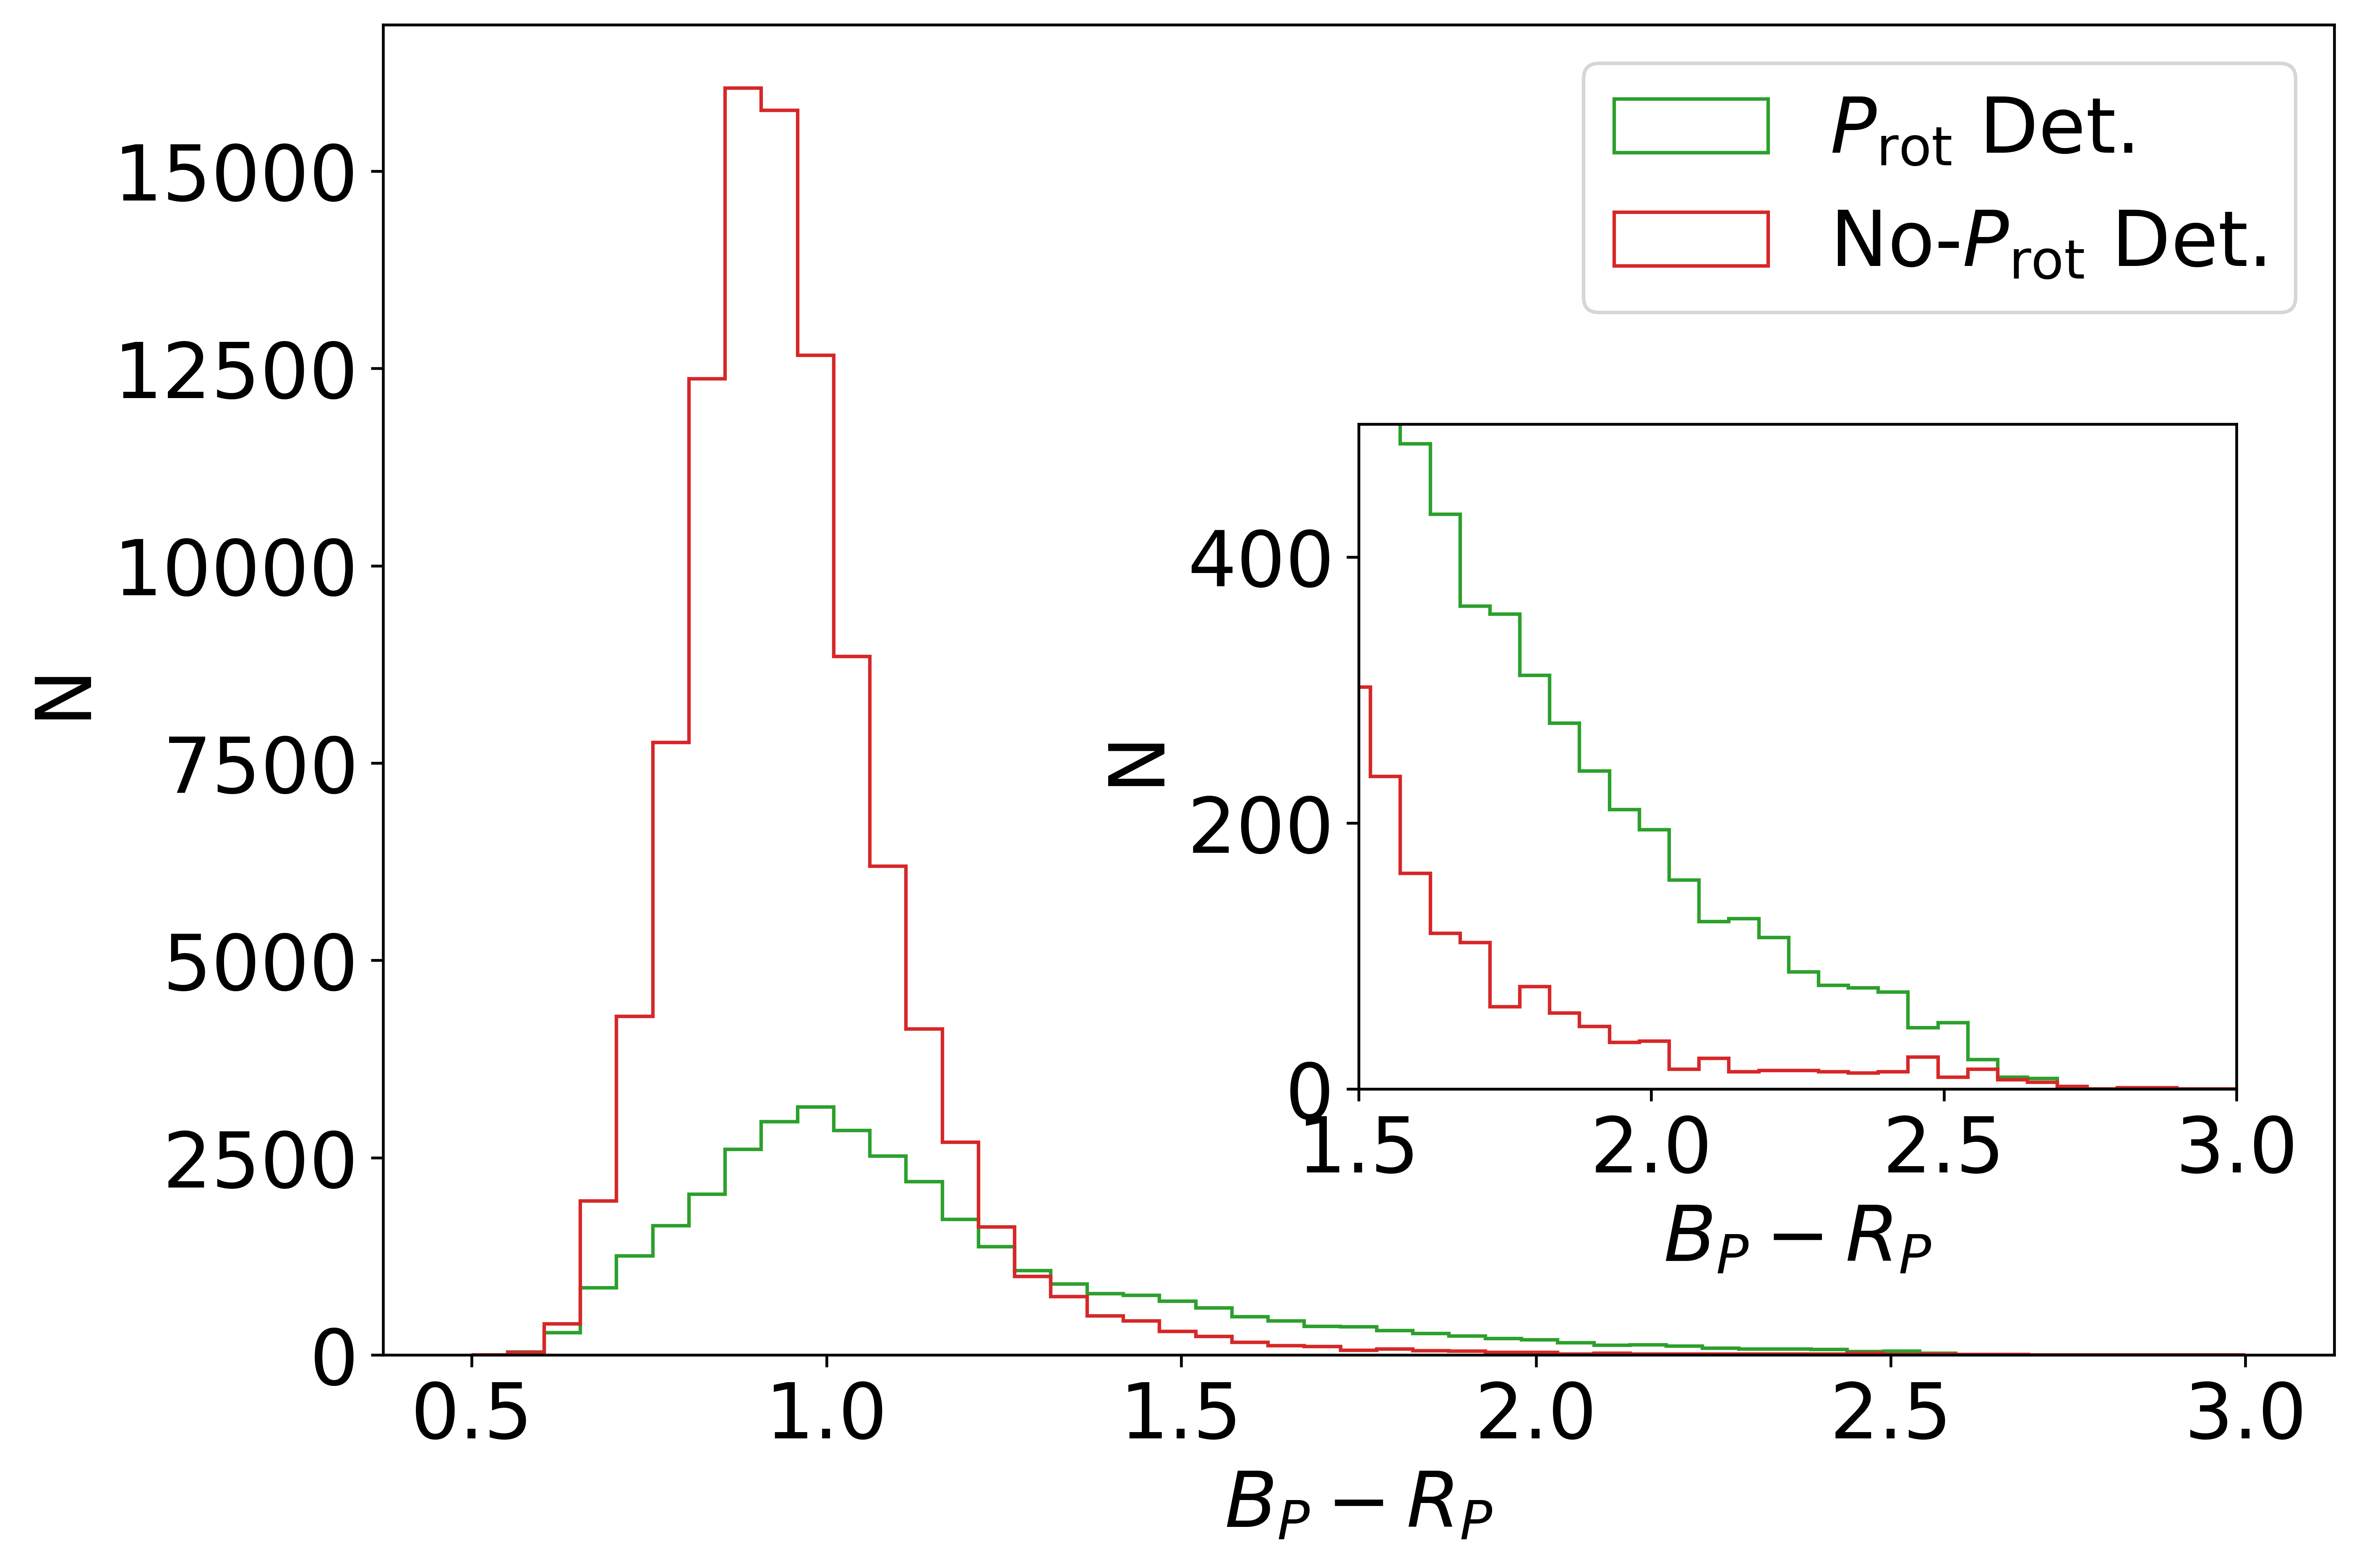
\includegraphics[width=\textwidth]{Figures/rot_gap_figures/hist_obs.png}
  \caption[A histogram of the distribution of $B_P-R_P$ colour of stars with (green) and without (red) detected rotation periods.]{A histogram of the distribution of $B_P-R_P$ colour of stars with (green) and without (red) detected rotation periods. \textbf{Inset:} A zoom-in of the distribution for $B_P-R_P\geq1.5$ where the rotational period gap is most apparent. The distribution in colour of stars with and without detected rotation periods vary. The undetected rotation sample is strongly biased towards stars with $B_P-R_P$ close to 1, comparative to the lower-mass stars where the number of stars drops quickly. Despite the $\sim$3:1 ratio of the number of stars with undetected rotation periods to those with detected rotation periods, the number of stars without detected rotation periods drops below those with detected rotation at $B_P-R_P\geq1.3$.
  	}
  \label{fig:n_det_nondet}
\end{figure}

We will more concretely investigate this by determining how many stars would be required to fill the gap - or rather for the dearth in observations to be undetectable in the low mass range where the proportion of stars between the samples is largest and where the gap is most apparent ($B_P-R_P$ $\geq$1.5).
To find the number of stars required for the dearth of observations to be no longer considered a dearth we first separate the sample with detected rotation into bins of $B_P - R_P$  from 1.5-2.2 of size 0.045 (15 bins).
In each colour interval, we then split the data into log rotational period intervals of width 0.07 dex between 1.0 and 1.7 dex (10 bins) which correspond to 10 and 50 days, respectively.
We then calculate the number of stars in each slice of log period for a given colour range.
In Figure \ref{fig:n_col} we show the number of stars in each slice (scatter points) against $\log_{10}$ of the rotation period for each colour range indicated in brackets to which we have fit a cubic spline (dashed).
From the cubic spline, we determine the position of the local minima in number of stars with detected rotation period, which is indicated by the solid vertical black line.
To calculate the number of stars required for the dearth, we compare the average of the two scatter bins surrounding the closest bin of the minima position.
While this approach is admittedly naive, as it assumes all of the stars will be in the bin closest to the minima rather than being distributed throughout the dearth region, it places a lower bound on the stars required to fill the gap.

\begin{figure}
\centering
  \includegraphics[width=\textwidth]{Figures/rot_gap_figures/n_col.png}
  \caption[Number of stars in each bin against $\log_{10}$ of the rotation period in bins of colour \gaia{} $B_P-R_P$.]{
  	Number of stars in each bin against $\log_{10}$ of the rotation period in bins of colour \gaia{} $B_P-R_P$ (indicated in brackets). Here we have fitted a cubic spline to the number of stars in each bin and calculated minima using the first and second derivatives of the fitted cubic spline. Solid vertical black lines show the minima in number of stars. These minima are the rotational period gap.
}
  \label{fig:n_col}
\end{figure}

In Figure \ref{fig:stars_not_fill} we compare the number of stars required to fill the gap to the number of stars without detected rotation periods in each colour range.
The number of stars required to fill the gap is approximately constant at N $\sim$ 20.
This suggests that the number of stars required to fill gap is independent of the total number of stars observed in that mass range.
Suppose, then, that the gap is full of stars without detectable rotation periods.
In that case, we expect the proportion of stars required to fill the gap to increase proportionate to the total number of stars (detected and non-detected rotation), but this is not the case.
The number of stars required to fill the gap is much smaller than the number of stars without detected rotation periods for $B_P-R_P<1.8$. 
Still, as colour increases and the number of observed (detected rotation period stars) stars decrease, the number of stars required to fill the gap becomes the majority of stars without detected rotation periods.
This suggests that for the gap to be full of stars with undetected rotational period stars, all of the stars in the undetected rotational period sample would need to be in this small rotational period range, and only a very small number of stars with undetected rotation are the result of noise or inclination effects.
The requirement of most (if not all) stars within the undetected rotation period sample suggests that the gap is not full of stars with undetectable rotation.

\begin{figure}
\centering
  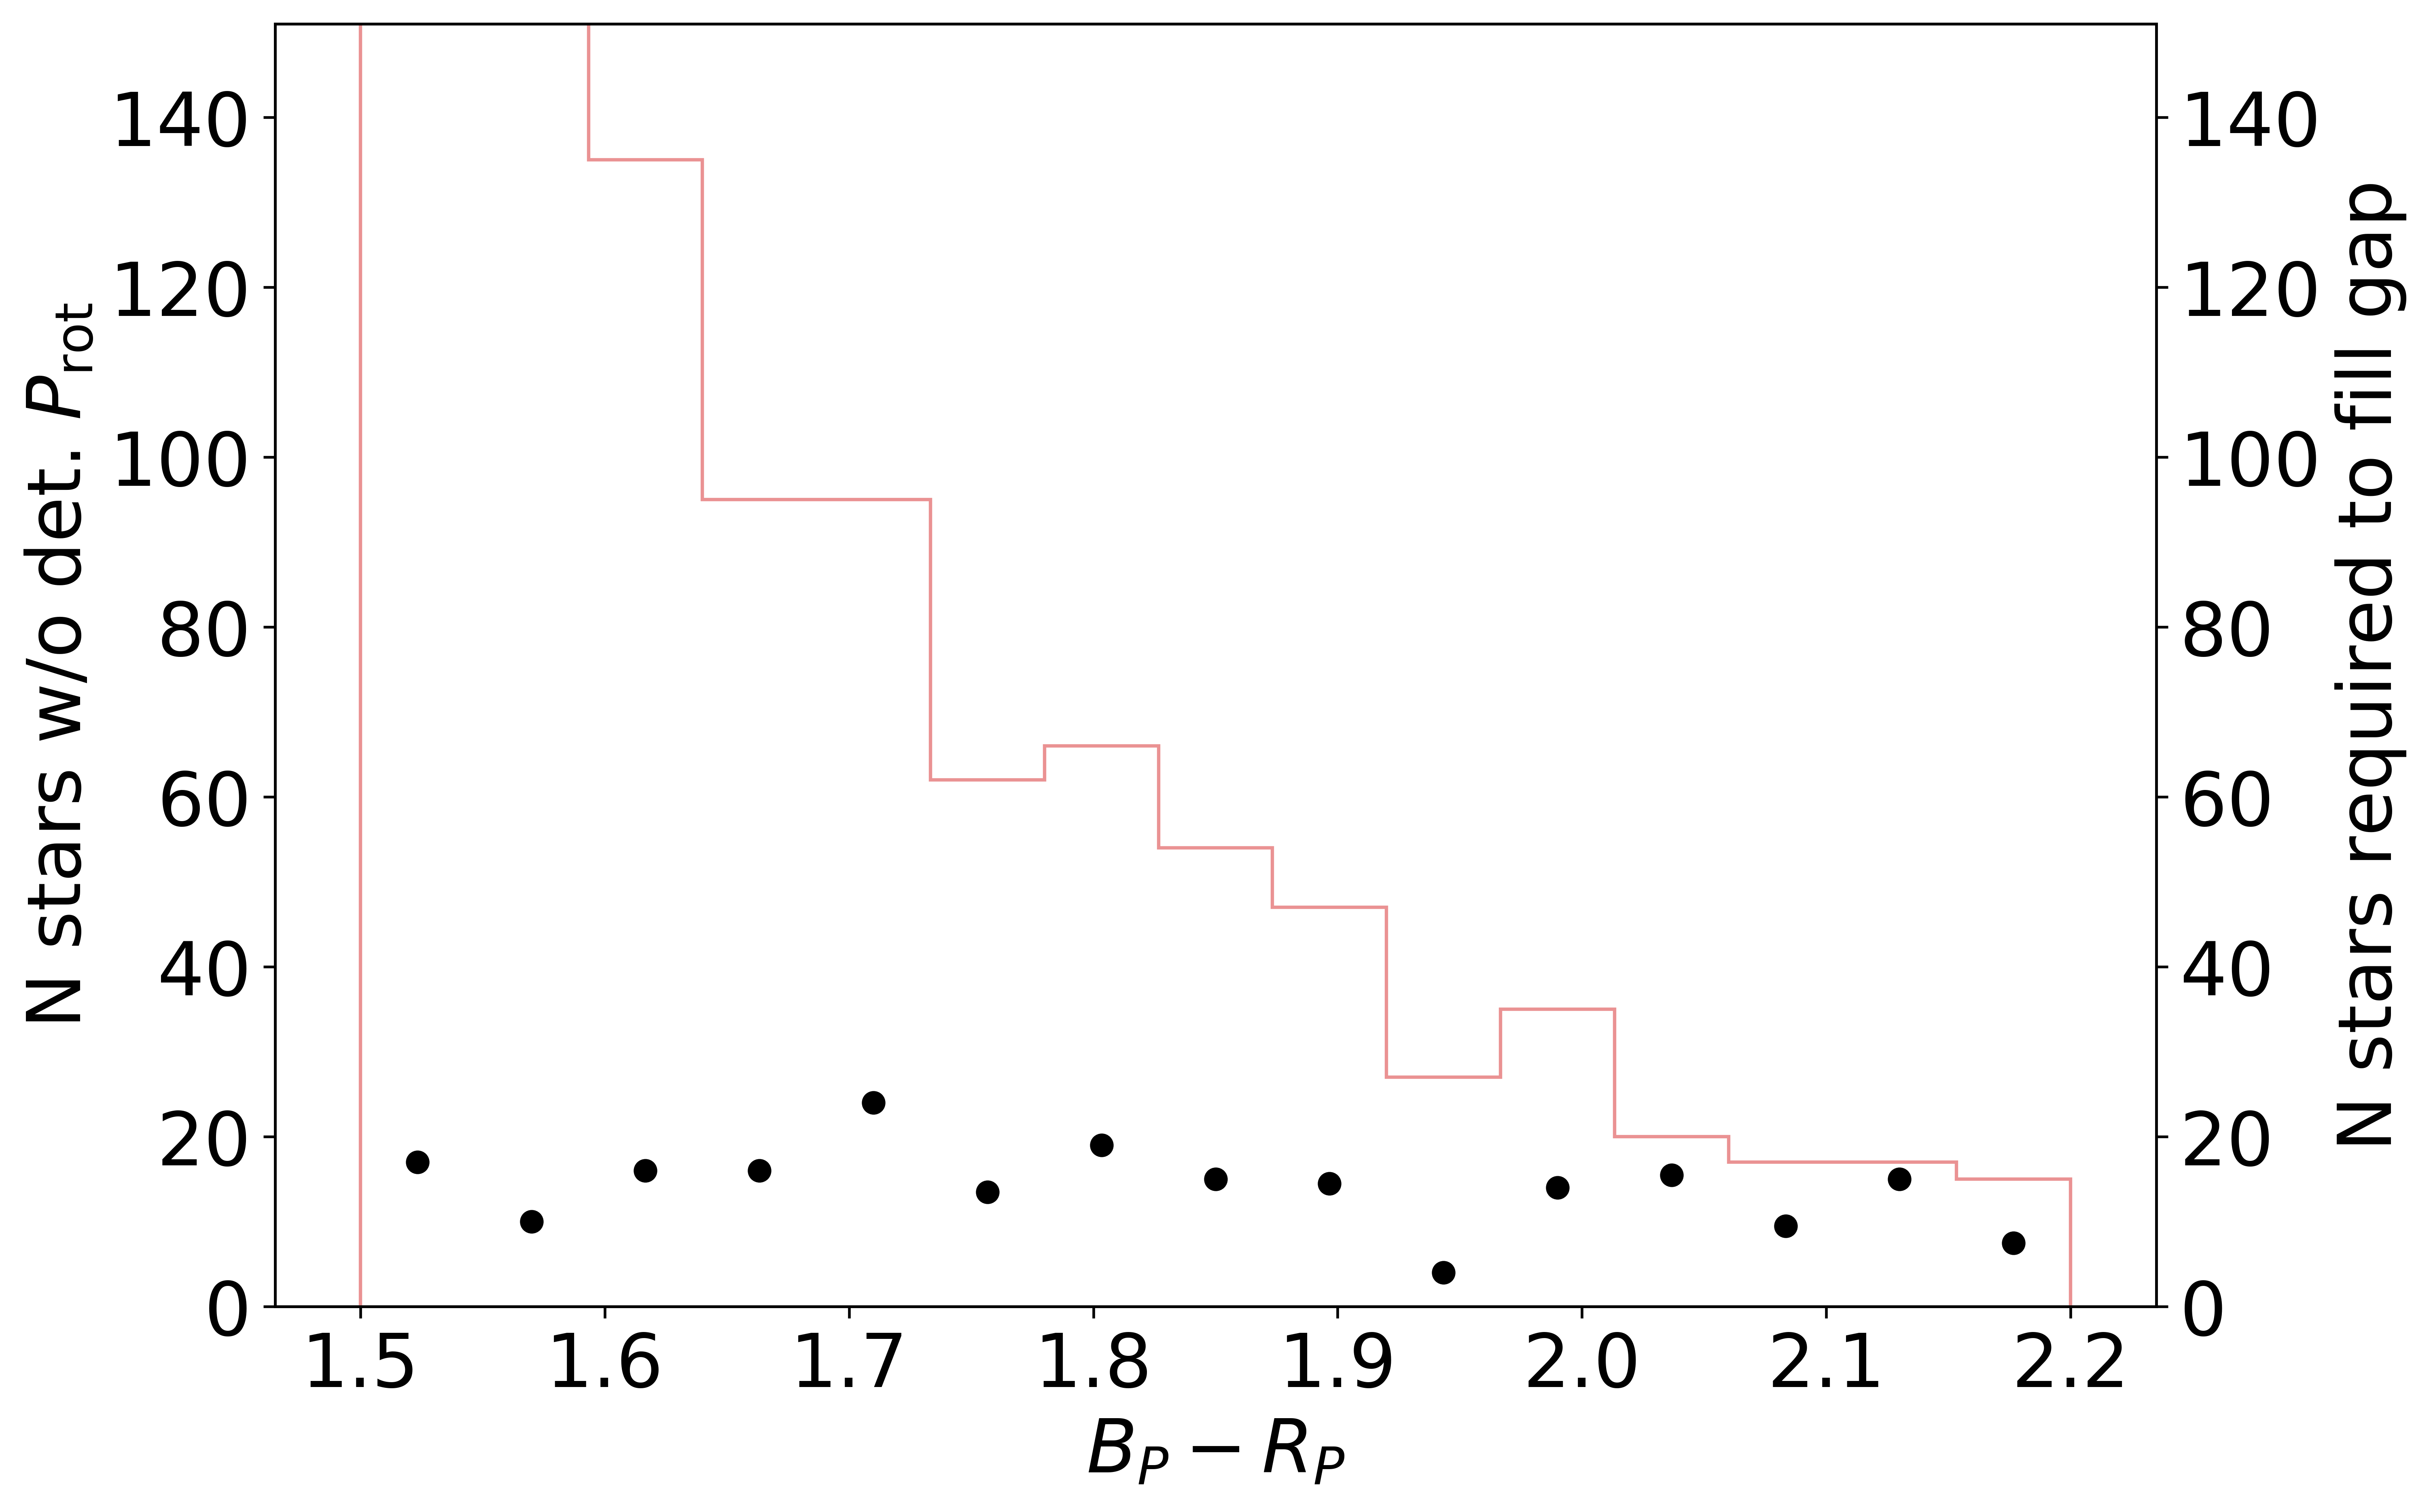
\includegraphics[width=\textwidth]{Figures/rot_gap_figures/stars_donot_fullgap.png}
  \caption[The number of stars required to fill the gap (black scatter points) against the number of stars with undetected rotation periods against $B_P-R_P$.]{
  	The number of stars required to fill the gap (black scatter points) against the number of stars with undetected rotation periods against $B_P-R_P$. The number of stars required to fill the intermediate period gap is roughly constant at N $\sim$ 20. While the number of stars without detected rotation greatly outnumbers the number required to fill the gap below $B_P-R_P \sim 1.8$, the two are almost equal for lower mass stars.
}
  \label{fig:stars_not_fill}
\end{figure}

\section{Summary and discussion}
\label{sec:summary}

Through this work we have reconfirmed that the gap aligns with a minima in the photometric variability range (\rper).
The coincidence of the gap and the minima has been invoked to suggest that the gap results from a very low probability of observing stars within the gap and that the gap is, in fact, full of stars with undetectable rotation periods.
The average \rper{} of stars around the gap does not fall below the detectability threshold of rotation and stars with much lower \rper{} have detectable rotation periods can be detected.

One explanation could be that \rper{} drops suddenly below the rotation detectability threshold, for stars precisely within the gap.
Th exact cause of this drop is unknown.
This drop could arise from a decrease in the magnetic activity of stars within the gap, leading to little to no expression of stellar spots or, as \citet{reinhold_transition_2019} suggests, the result of the cancellation brightness variations of spots by faculae 
We found in this work that the drop in \rper{}, and thus the gap, is also coincident with a drop in $\log R^{+}_{\rm{HK}}$ suggesting that the decrease in photometric variability in stars close to the gap is the result of a decrease in magnetic activity, rather than a transition in the spots dominance to faculae dominance.
However, we also found that there is not a subsample of stars without rotational period detection but with ultra-low $\log R^{+}_{\rm{HK}}$.
While the stars without rotational period detection tend to have lower magnetic activity, there is not an obvious subsample of stars with $\log R^{+}_{\rm{HK}}$ below the rotation period detection threshold.
This suggests that there are no stars within the gap with ultra-low magnetic activity that make rotational period observation impossible.

Another possible mechanism we can investigate using this data arises if we consider that stars within the gap may have magnetic activity so great that noise dominates their light curves making observation of their rotation impossible.
Rotation tends to be less readily detectable at high activity when the light curve is noisy from the stochastic production of a larger number of surface features.
Consider a scenario whereby the average magnetic activity of stars increases in the region of evolution around the magnetic activity gap. 
Indeed, the magnetic activity of stars tends to decrease with rotation rate, but we will ignore this for now.
Let us assume instead that the spot-faculae cancellation does not occur and that brightness variations on a magnetic activity timescale are spot dominated below the Vaughn-Preston Gap \footnote{A distinct gap from the intermediate period gap wherein the transition from spot dominance to faculae dominance occurs in their work}.
Conceivably, as the average magnetic activity increases for stars near the gap, the regions where noise is minimal enough for rotation to be detected become smaller and more concentrated to times when the magnetic activity of stars is very small, which must constitute a minority of stars for a given $B_P-R_P$ and rotational period.
This would coincide with a decrease in \rper{} of stars as average magnetic activity increases.
The gap would then represent a region of evolution where the average magnetic activity of stars would be large enough that the noise permeates the entire magnetic activity cycle, and no rotation observations could be made.
Observations of rotation period should therefore be more likely to occur when a star is minimally active and thus has the smallest observed magnetic activity- which would also correspond to a minima in observed $\log R^{+}_{\rm{HK}}$.
This would suggest that there is a population of magnetically active stars with $\log R^{+}_{\rm{HK}}$ greater than the average magnetic activity of stars near the gap that have otherwise undetectable rotation periods.
In Figure \ref{fig:detection_efficiency_rhk}, we show that there is not a subsample low rotation detectability stars with $\log R^{+}_{\rm{HK}}$ greater than the average of stars near the rotational period gap, suggesting that this selection mechanism is not at play.

The proposition that the rotational period gap represents a minimum of detectability of stars is not favoured by the data.
The coincidence of the minima in \rper{} with minima in $\log R^{+}_{\rm{HK}}$ along with the lack of a population of low or high $\log R^{+}_{\rm{HK}}$ stars with low detectability suggests that minima in \rper{} cannot be explained by a spot-faculae transition nor a selection effect for stars with low or high magnetic activity near the rotational period gap.
Furthermore, we found that for the gap to be explained by a lack of detection of the rotational period, stars within the gap must make up most stars in the \kepler{} non-detected rotational period sample.
This explanation is unlikely due to the many factors by which rotation is not observed for all stars: inclination effects, noise drowning the rotational period signal etc.
Recent works have also tentatively shown that the kinematic ages of stars above and below the rotation period gap have comparable kinematic ages \citep{lu_bridging_2022} which suggests that there is no missing sample of stars that fill the gap.

The only alternative mechanism that has been proposed in the literature is the onset of strong surface angular momentum loss whereby stars ``jump" the gap.
However, this explanation does not have a proposed physical mechanism.
As stars evolve toward the gap, their core and envelope undergo recoupling, slowing their spin-down.
\citet{cao_core-envelope_2023} suggest that the process of core-envelope recoupling with significant angular momentum flux (See Section 4. of their work) between the core and the surface enhances the magnetic dynamo of stars, inducing larger photometric variability from greater spot coverage.
The decrease in photometric variability towards the gap can be explained under this framework if the enhancement of the magnetic dynamo is dependent on the scale of the radial shear between the core and the surface, which decreases towards the gap if the core and envelope have completely recoupled.

Two mechanisms could then be invoked to explain the sudden enhanced spin-down: core-envelope re-decoupling or enhanced magnetic spin-down.
Conceivably the core and the surface of the star can again decouple at the rotational period gap; the surface spins down at a much faster rate than below the gap resulting in the apparent dearth of observations.
It is, however, not clear the effect that this decoupling would have above the gap.
If the core and envelope are strongly decoupled above the gap then angular momentum transport between the core and surface is likely to reoccur, supported by the relatively flat radial differential rotation profile observed for the Sun and young subgiants \citep{deheuvels_seismic_2015}.
\rper{} of stars just above the gap is similar to stars below the gap, suggesting that they do not have enhanced dynamos consistent with the strong radial shears.
\rper{} increases with rotation period above the gap, suggesting instead that the enhancement of the dynamo by core-envelope should grow as the star evolves.
For this to be the case the core-surface radial shear must grow and the core and surface must remain decoupled until recoupling enhances the magnetic dynamo.
However, the gap is only apparent for a small rotational period range and the density of stars with observed rotation periods above and below the gap are consistent - suggesting that the decoupling is not slowly counteracted by core-envelope recoupling resulting in the enhanced \rper{} away from the gap.

Enhanced magnetic angular momentum loss is another possible explanation for the gap.
The magnetic braking of a star is dependent on the rotation rate, mass loss rate and the strength of the magnetic field.
Stars near and just above the gap are rotating slower and have smaller magnetic activity indicators than stars below the gap.
Further, we found that stars just above the gap do not show significant enhancement in $\log R^{+}_{\rm{HK}}$.
If the sudden increase in magnetic braking arises from enhancement to the magnetic field, it is not reflected in the magnetic activity of stars near the gap.
The only other variable to consider here is increased mass loss.
While mass loss rates of main-sequence stars are an ongoing field of research, to reflect the change in rotation period of stars passing through the gap, we speculate that the mass loss rate would need to be enhanced by several orders of magnitude compared to the observed mass loss rate of the Sun. 
That significant mass loss is not reflected in any other measurements of stars surrounding the gap, nor is there a known mechanism by which the enhanced mass loss would occur.
As a result, currently, there is no known mechanism for said enhanced magnetic braking to arise.

\section{Conclusion}
\label{sec:conclusion}

In this work we have proposed that the data does not support the two leading explanations for the intermediate period gap: a sudden decrease in probability of rotational period detection or the sudden onset magnetic braking.
While further work is required to definitively rule out their involvement in the intermediate period gap, we use this as motivation to propose a novel explanation for the intermediate period gap: the sudden onset of latitudinal differential rotation and the impact that has on the observed rotational periods of stars.

We thank Jing Hua Zhang for providing us with the magnetic activity indicators $\log \ R^{+}_{\rm{HK}}$ and $S$ values of the non-rotating sample of the \kepler-\lamost\ crossmatch in their work \citet{zhang_magnetic_2020} that made sections of this work possible.


	% Appendix Title
%
%%\input{Appendices/AppendixB} % Appendix Title
%
%%\input{Appendices/AppendixC} % Appendix Title
%
%\addtocontents{toc}{\vspace{2em}}  % Add a gap in the Contents, for aesthetics
%\backmatter

%% ----------------------------------------------------------------
\label{Bibliography}
\lhead{\emph{Bibliography}}  % Change the left side page header to "Bibliography"
\bibliographystyle{mnras}  % Use the "unsrtnat" BibTeX style for formatting the Bibliography
\bibliography{references}  % The references (bibliography) information are stored in the file named "Bibliography.bib"

\end{document}  % The End
%% ----------------------------------------------------------------